%
% generate PDF file
% pdflatex solnQCQI.tex
%
\documentclass[11pt]{book}
\usepackage[utf8]{inputenc}
\usepackage{amsmath,amsfonts,amssymb,amsthm}
\usepackage{enumitem}
\usepackage[letterpaper,left=0.5in,top=0.65in,bottom=0.65in]{geometry}
\usepackage[dvipdfmx]{graphicx}
\usepackage[english]{babel}
 
%図の場所をなるべく指定した場所にする
\usepackage{booktabs}
\usepackage{here}

\RequirePackage[l2tabu, orthodox]{nag}
%\usepackage[all, warning]{onlyamsmath}

%単位を書くときに使う
\usepackage{siunitx}

\usepackage{CJKutf8}
\usepackage{ascmac} % screen
\usepackage{ulem}
\usepackage{cases}
\usepackage{braket}
\usepackage{dsfont}
\usepackage{ascmac}
\usepackage{url}
\PassOptionsToPackage{hyphens}{url}\usepackage{hyperref} % hyper link
\usepackage{ccicons} % creative commons license icon
\usepackage{fancyhdr} % footer
\usepackage{blkarray}
%\pagestyle{fancy}
%\cfoot[\href{http://creativecommons.org/licenses/by-nc-sa/4.0/}{Creative Commons Attribution-NonCommercial-ShareAlike 4.0 International License}.]{}
\usepackage{color}
\usepackage{calc}
\usepackage{stmaryrd}
\usepackage{adjustbox}
\usepackage{lscape}
\usepackage{tocloft}
\usepackage{comment}
\usepackage{changepage}

\usepackage{tikz}
\usepackage{circuitikz}
\usetikzlibrary{decorations.pathreplacing,decorations.pathmorphing}

%\usepackage{xcolor}
%\definecolor{Pagecolor}{RGB}{35,38,41} % Dark gray
%\definecolor{Textcolor}{RGB}{255,255,255} % Light gray
%\pagecolor{Pagecolor}
%\color{Textcolor}

\usepackage[T1]{fontenc}
\usepackage{lmodern}

%\newcommand{\Gate}[1]{{\fontfamily{pcr}\selectfont#1}}
\newcommand{\NAND}{{\fontfamily{pcr}\selectfont NAND}}
\newcommand{\AND}{{\fontfamily{pcr}\selectfont AND}}
\newcommand{\OR}{{\fontfamily{pcr}\selectfont OR}}
\newcommand{\NOR}{{\fontfamily{pcr}\selectfont NOR}}
\newcommand{\NOT}{{\fontfamily{pcr}\selectfont NOT}}
\newcommand{\XOR}{{\fontfamily{pcr}\selectfont XOR}}
\newcommand{\FANOUT}{{\fontfamily{pcr}\selectfont FANOUT}}
\newcommand{\CROSSOVER}{{\fontfamily{pcr}\selectfont CROSSOVER}}
\newcommand{\CNOT}{{\fontfamily{pcr}\selectfont CNOT}}

\newcommand\encircle[1]{%
  \tikz[baseline=(X.base)] 
    \node (X) [draw, shape=circle, inner sep=0] {\strut #1};}


\usepackage{mathtools}
\DeclarePairedDelimiter\Abs{\lvert}{\rvert}
\DeclarePairedDelimiter\Ceil{\lceil}{\rceil}
\DeclarePairedDelimiter\Floor{\lfloor}{\rfloor}
\newcommand{\abs}[1]{\Abs*{#1}}
\newcommand{\ceil}[1]{\Ceil*{#1}}
\newcommand{\floor}[1]{\Floor*{#1}}
%\newcommand{\abs}[1]{\big|#1\big|}
%\newcommand{\ceil}[1]{\left\lceil#1\right\rceil}
%\newcommand{\floor}[1]{\left\lfloor#1\right\rfloor}

%\renewcommand{\familydefault}{\sfdefault}
%% Only use the math font of mathpazo
%\let\temp\rmdefault
%\usepackage{fourier}
%\let\rmdefault\temp

\usepackage{fancyhdr}
\setlength{\headheight}{15.2pt}
\pagestyle{fancy}
\lhead[\leftmark ]{\thepage}
\rhead[\thepage]{\leftmark}

\cfoot{\footnotesize \textcopyright 2018 goropikari, \textcopyright 2021 tlesaul2 - \href{http://creativecommons.org/licenses/by-nc-sa/4.0/}{Creative Commons Attribution-NonCommercial-ShareAlike 4.0 International License}}

% コマンド定義
\DeclareMathOperator{\Tr}{tr} 
\newcommand{\norm}[1]{\left\lVert#1\right\rVert} % norm ||x||
\newcommand{\kb}[1]{\ket{#1}\hspace{-1mm} \bra{#1}} % |x><x|
\newcommand{\kbt}[2]{\ket{#1}\hspace{-1mm} \bra{#2}} % |x><y|
\newcommand{\Textbf}[1]{\hspace{3mm}\\\textbf{#1)}}
\newcommand{\Soln}{\textbf{\\Soln: }}
\newcommand{\Mod}[1]{\ (\mathrm{mod}\ #1)}
\newtheorem{thm}{Theorem.}[section]
\newtheorem{prop}{Proposition.}[section]



\title{Select Solutions for ``Quantum Computation and Quantum Information: 10th Anniversary Edition'' by Nielsen and Chuang}
\author{Original author: goropikari\\Extended by: tlesaul2}
\date{\today}

\let\tmp\oddsidemargin
\let\oddsidemargin\evensidemargin
\let\evensidemargin\tmp
\reversemarginpar

\let\Re\undefined
\let\Im\undefined
\DeclareMathOperator{\Re}{\mathfrak{Re}}
\DeclareMathOperator{\Im}{\mathfrak{Im}}

\begin{document}
\maketitle
\thispagestyle{empty}
\cleardoublepage
\thispagestyle{empty}
\setcounter{page}{1} % 表紙のページを0ページにする

\section*{Copylight Notice:}
\ccbyncsa\\
    This work is licensed under a \href{http://creativecommons.org/licenses/by-nc-sa/4.0/}{Creative Commons Attribution-NonCommercial-ShareAlike 4.0 International License} by the original author.  As such, the second author does the same.


\section*{Repository}
As of November, 2021, the original source \LaTeX \ code, located at \url{https://github.com/goropikari/SolutionForQuantumComputationAndQuantumInformation}\ has not been updated since April 2020.  The extended source \LaTeX \ code is located at \\ \url{https://github.com/tlesaul2/SolutionQCQINielsenChuang}\ .  It may be updated more actively.

\section*{For readers}
This is an unofficial solution manual for "\href{http://www.cambridge.org/jp/academic/subjects/physics/quantum-physics-quantum-information-and-quantum-computation/quantum-computation-and-quantum-information-10th-anniversary-edition?format=HB&isbn=9781107002173#BBFv83H3ofgcgG3A.97}{Quantum Computation and Quantum Information: 10th Anniversary Edition}" (ISBN-13: 978-1107002173) by Michael A. Nielsen and Isaac L. Chuang.\\

\noindent From the original author:\\
\indent I have studied quantum information theory as a hobby.
And I'm not a researcher.
So there is no guarantee that these solutions are correct.
Especially because I'm not good at mathematics, proofs are often wrong.
Don't trust me. Verify yourself!

If you find some mistake or have some comments, please feel free to open an issue or a PR.
\begin{flushright}
\href{https://github.com/goropikari}{goropikari}\\
\end{flushright}

\noindent From the second author:\\
\indent I'm a mathematician relatively new to quantum information theory as of the adoption of this repo, so hope to supplement the original author's work by checking and formalizing the mathematics, overly at times, while I use the task to learn the field.  The original author's sentiments about self-verification are echoed.
\begin{flushright}
\href{https://github.com/tlesaul2}{tlesaul2}
\end{flushright}

\clearpage

{\let\cleardoublepage\clearpage\tableofcontents\thispagestyle{empty}}

%%%%%%%%%%%%%%%%%%%%%%%%%%%%%%%%%%%%%%%%%%%%%%%%%%%%%%%%%%%%%%%%%%%%%%%%%%%%%

\frontmatter
\chapter{Errata list}\label{errata}

\begin{itemize}
    \item p.101. eq (2.150) $\rho = \sum_m p(m) \rho_m$ should be $\rho \textcolor{red}{'} = \sum_m p(m) \rho_m$.
%
  \item p.103. Exercise 2.26. Show that the circuit:
\begin{center}
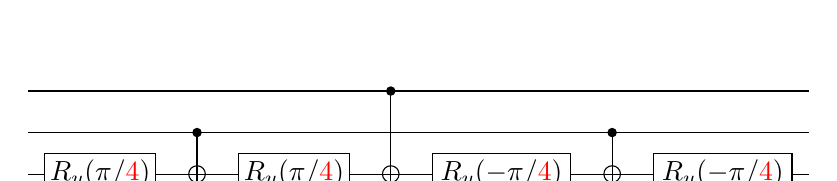
\begin{tikzpicture}[scale=1.000000,x=1pt,y=1pt]
\filldraw[color=white] (0.000000, -7.500000) rectangle (282.000000, 37.500000);
% Drawing wires
% Line 1: a3 W
\draw[color=black] (0.000000,30.000000) -- (282.000000,30.000000);
% Line 2: a2 W
\draw[color=black] (0.000000,15.000000) -- (282.000000,15.000000);
% Line 3: a1 W
\draw[color=black] (0.000000,0.000000) -- (282.000000,0.000000);
% Done with wires; drawing gates
% Line 4: a1 G $R_y(\pi/\textcolor{red}{4})$ width=40 height=15
\begin{scope}
\draw[fill=white] (26.000000, -0.000000) +(-45.000000:28.284271pt and 10.606602pt) -- +(45.000000:28.284271pt and 10.606602pt) -- +(135.000000:28.284271pt and 10.606602pt) -- +(225.000000:28.284271pt and 10.606602pt) -- cycle;
\clip (26.000000, -0.000000) +(-45.000000:28.284271pt and 10.606602pt) -- +(45.000000:28.284271pt and 10.606602pt) -- +(135.000000:28.284271pt and 10.606602pt) -- +(225.000000:28.284271pt and 10.606602pt) -- cycle;
\draw (26.000000, -0.000000) node {$R_y(\pi/\textcolor{red}{4})$};
\end{scope}
% Line 5: +a1 a2
\draw (61.000000,15.000000) -- (61.000000,0.000000);
\begin{scope}
\draw[fill=white] (61.000000, 0.000000) circle(3.000000pt);
\clip (61.000000, 0.000000) circle(3.000000pt);
\draw (58.000000, 0.000000) -- (64.000000, 0.000000);
\draw (61.000000, -3.000000) -- (61.000000, 3.000000);
\end{scope}
\filldraw (61.000000, 15.000000) circle(1.500000pt);
% Line 6: a1 G $R_y(\pi/\textcolor{red}{4})$ width=40 height=15
\begin{scope}
\draw[fill=white] (96.000000, -0.000000) +(-45.000000:28.284271pt and 10.606602pt) -- +(45.000000:28.284271pt and 10.606602pt) -- +(135.000000:28.284271pt and 10.606602pt) -- +(225.000000:28.284271pt and 10.606602pt) -- cycle;
\clip (96.000000, -0.000000) +(-45.000000:28.284271pt and 10.606602pt) -- +(45.000000:28.284271pt and 10.606602pt) -- +(135.000000:28.284271pt and 10.606602pt) -- +(225.000000:28.284271pt and 10.606602pt) -- cycle;
\draw (96.000000, -0.000000) node {$R_y(\pi/\textcolor{red}{4})$};
\end{scope}
% Line 7: +a1 a3
\draw (131.000000,30.000000) -- (131.000000,0.000000);
\begin{scope}
\draw[fill=white] (131.000000, 0.000000) circle(3.000000pt);
\clip (131.000000, 0.000000) circle(3.000000pt);
\draw (128.000000, 0.000000) -- (134.000000, 0.000000);
\draw (131.000000, -3.000000) -- (131.000000, 3.000000);
\end{scope}
\filldraw (131.000000, 30.000000) circle(1.500000pt);
% Line 8: a1 G $R_y(-\pi/\textcolor{red}{4})$ width=50 height=15
\begin{scope}
\draw[fill=white] (171.000000, -0.000000) +(-45.000000:35.355339pt and 10.606602pt) -- +(45.000000:35.355339pt and 10.606602pt) -- +(135.000000:35.355339pt and 10.606602pt) -- +(225.000000:35.355339pt and 10.606602pt) -- cycle;
\clip (171.000000, -0.000000) +(-45.000000:35.355339pt and 10.606602pt) -- +(45.000000:35.355339pt and 10.606602pt) -- +(135.000000:35.355339pt and 10.606602pt) -- +(225.000000:35.355339pt and 10.606602pt) -- cycle;
\draw (171.000000, -0.000000) node {$R_y(-\pi/\textcolor{red}{4})$};
\end{scope}
% Line 9: +a1 a2
\draw (211.000000,15.000000) -- (211.000000,0.000000);
\begin{scope}
\draw[fill=white] (211.000000, 0.000000) circle(3.000000pt);
\clip (211.000000, 0.000000) circle(3.000000pt);
\draw (208.000000, 0.000000) -- (214.000000, 0.000000);
\draw (211.000000, -3.000000) -- (211.000000, 3.000000);
\end{scope}
\filldraw (211.000000, 15.000000) circle(1.500000pt);
% Line 10: a1 G $R_y(-\pi/\textcolor{red}{4})$ width=50 height=15
\begin{scope}
\draw[fill=white] (251.000000, -0.000000) +(-45.000000:35.355339pt and 10.606602pt) -- +(45.000000:35.355339pt and 10.606602pt) -- +(135.000000:35.355339pt and 10.606602pt) -- +(225.000000:35.355339pt and 10.606602pt) -- cycle;
\clip (251.000000, -0.000000) +(-45.000000:35.355339pt and 10.606602pt) -- +(45.000000:35.355339pt and 10.606602pt) -- +(135.000000:35.355339pt and 10.606602pt) -- +(225.000000:35.355339pt and 10.606602pt) -- cycle;
\draw (251.000000, -0.000000) node {$R_y(-\pi/\textcolor{red}{4})$};
\end{scope}
% Done with gates; drawing ending labels
% Done with ending labels; drawing cut lines and comments
% Done with comments
\end{tikzpicture}
\end{center}
\vspace{-5pt}
differs from a Toffoli gate only by relative phases.

    \item p.408. eq (9.49) $\sum_i p_i D(\rho_i, \sigma_i) + D(p_i, q_i)$ should be $\sum_i p_i D(\rho_i, \sigma_i) + \textcolor[rgb]{1,0,0}{2}D(p_i, q_i)$.

    \begin{align*}
    \text{eqn } (9.48) 
        &= \sum_i p_i \Tr (P(\rho_i - \sigma_i)) + \sum_i (p_i - q_i) \Tr (P \sigma_i)\\
        &\leq \sum_i p_i \Tr (P(\rho_i - \sigma_i)) + \sum_i |p_i - q_i| \Tr (P \sigma_i)~~~(\because p_i - q_i \leq |p_i - q_i|)\\
        &\leq \sum_i p_i \Tr (P(\rho_i - \sigma_i)) + \sum_i |p_i - q_i|~~~(\because \Tr (P \sigma_i) \leq 1)\\
        &= \sum_i p_i \Tr (P(\rho_i - \sigma_i)) + 2 \frac{\sum_i |p_i - q_i|}{2}\\
        &= \sum_i p_i \Tr (P(\rho_i - \sigma_i)) + 2D(p_i, q_i)
    \end{align*}
%
    \item p.409. Exercise 9.12. If $\rho = \sigma$, then $D(\rho, \sigma) = 0$. Furthermore trace distance is non-negative. Therefore $0 \leq D(\mathcal{E}(\rho), \mathcal{E}(\sigma)) \leq 0 \Rightarrow D(\mathcal{E}(\rho), \mathcal{E}(\sigma))  = 0$. So I think the map $\mathcal{E}$ is not strictly contractive. If $p \neq 1$ and $\rho \neq \sigma$, then $D(\mathcal{E}(\rho), \mathcal{E}(\sigma)) < D(\rho, \sigma)$ is satisfied.
%
    \item p.411. Exercise 9.16. eqn(9.73) $\Tr (A^\dagger B) = \braket{m | A \otimes B | m}$ should be $\Tr (A^{\textcolor{red}{T}} B) = \braket{m | A \otimes B | m}$.

    Simple counter example is the case that
    $A = \begin{bmatrix}
        i & 0\\
        0 & 0
    \end{bmatrix}$.
    $B = \begin{bmatrix}
        1 & 0\\
        0 & 0
    \end{bmatrix}$,
    In this case,
    \begin{align*}
        A^\dagger B &=
        \begin{bmatrix}
            -i & 0\\
            0 & 0
        \end{bmatrix}
        \begin{bmatrix}
            1 & 0\\
            0 & 0
        \end{bmatrix}
        = \begin{bmatrix}
            -i & 0\\
            0 & 0
        \end{bmatrix},\\
%
        \Tr (A^\dagger B)& = -i,\\
%
        A \otimes B &= \begin{bmatrix}
            i & 0 & 0 & 0\\
            0 & 0 & 0 & 0\\
            0 & 0 & 0 & 0\\
            0 & 0 & 0 & 0
        \end{bmatrix}\\
        \braket{m | A \otimes B | m} &= (\bra{00} + \braket{11}) (A \otimes B) (\ket{00} + \ket{11}) = i.
    \end{align*}
    Thus $\Tr(A^\dagger B) \neq \braket{m | A \otimes B | m}$.

    By using following relation, we can prove.
    \begin{align*}
        (I \otimes A) \ket{m} = (A^T \otimes I) \ket{m}\\
        \Tr (A) = \braket{m | I \otimes A | m}
    \end{align*}
%
    \begin{align*}
        \Tr (A^T B) = \Tr(BA^T) &= \braket{m | I \otimes BA^T |m}\\
            &= \braket{m | (I \otimes B)(I \otimes A^T) |m}\\
            &= \braket{m | (I \otimes B)(A \otimes I) |m}\\ 
            &= \braket{m | A \otimes B | m}.
    \end{align*}

    \item p.515. eqn (11.67) $S(\rho' || \rho)$ should be $S(\rho || \rho \textcolor{red}{'})$.
\end{itemize}


\mainmatter
\setcounter{chapter}{1}
%!TeX root=../solnQCQI.tex

\chapter{Introduction to quantum mechanics}
\Textbf{2.1} Show that $(1, -1), (1,2)$, and $(2,1)$ are linearly dependent.
\Soln It is enough to express $(0, 0)$ as a linear combination of the specified vectors.
\begin{align*}
	\begin{bmatrix}
		1 \\
		-1
	\end{bmatrix}
	+
	\begin{bmatrix}
		1 \\
		2
	\end{bmatrix}
	-
	\begin{bmatrix}
		2 \\
		1
	\end{bmatrix}
	=
	\begin{bmatrix}
		0 \\
		0
	\end{bmatrix}
\end{align*}

\Textbf{2.2} Suppose $V$ is a vector space with basis vectors $\ket{0}$ and $\ket{1}$, and $A$ is a linear operator
from $V$ to $V$ such that $A\ket{0}=\ket{1}$ and $A\ket{1}=\ket{0}$.  Give a matrix representation for $A$, with
respect to the input bais $\ket{0},\ket{1}$, and the output basis $\ket{0},\ket{1}$.  Find input and output bases which
give rise to a different matrix representation of $A$.
\Soln With specified operations, it is enough to solve for the entries of a 2x2 matrix which
coverts the input vectors expressed as linear combinations of one basis, say $(\ket{a_1},\ket{a_2}),$
into vectors expressed as linear combinations of another basis, say $(\ket{b_1},\ket{b_2})$.
\[
A = \begin{blockarray}{ccc}
\begin{block}{ccc}
& \ket{b_1} & \ket{b_2}\\
    \end{block}
\begin{block}{ c[cc] }
\ket{a_1} & A_{11} & A_{12} \\
\ket{a_2} & A_{21} & A_{22} \\
            \end{block}
        \end{blockarray}
\]
With $(\ket{a_1},\ket{a_2}) = (\ket{0},\ket{1})$ and $(\ket{b_1},\ket{b_2}) = (\ket{0},\ket{1})$, we have
\begin{align*}
	A\ket{0} &:= \ket{1} = 0\ket{0}+1\ket{1}= A_{11}\ket{b_1} + A_{21}\ket{b_2} = A_{11}\ket{0} + A_{21}\ket{1}\Rightarrow A_{11} = 0,\ A_{21} = 1\\
	A\ket{1} &:= \ket{0} = 1\ket{0}+0\ket{1}=A_{12}\ket{b_1} + A_{22}\ket{b_2} = A_{12}\ket{0} + A_{22}\ket{1}\Rightarrow A_{12} = 1,\ A_{22} = 0\\
%
	\therefore A &=
	\begin{bmatrix}
		0 & 1 \\
		1 & 0
	\end{bmatrix}
\end{align*}
If the output basis was $(\ket{b_1},\ket{b_2}) = (\ket{1},\ket{0})$ instead, then $A=I$.  More formally:
\begin{align*}
    A\ket{0} &:= \ket{1} = 1\ket{1}+0\ket{0}= A_{11}\ket{b_1} + A_{21}\ket{b_2} = A_{11}\ket{1} + A_{21}\ket{0}\Rightarrow A_{11} = 1,\ A_{21} = 0\\
    A\ket{1} &:= \ket{0} = 0\ket{1}+1\ket{0}= A_{12}\ket{b_1} + A_{22}\ket{b_2} = A_{12}\ket{1} + A_{22}\ket{0}\Rightarrow A_{12} = 0,\ A_{22} = 1\\
        %
    \therefore A &=
    \begin{bmatrix}
    1 & 0 \\
    0 & 1
    \end{bmatrix}
\end{align*}
With a more interesting orthonormal output basis $(\ket{b_1},\ket{b_2})=(\ket{+},\ket{-})$:
\begin{align*}
        A\ket{0} &:= \ket{1} = \frac{\sqrt{2}}{2}\ket{+}-\frac{\sqrt{2}}{2}\ket{-}= A_{11}\ket{b_1} + A_{21}\ket{b_2} = A_{11}\ket{+} + A_{21}\ket{-}\Rightarrow A_{11} = \frac{\sqrt{2}}{2},\ A_{2} = -\frac{\sqrt{2}}{2}\\
        A\ket{1} &:= \ket{0} = \frac{\sqrt{2}}{2}\ket{+}+\frac{\sqrt{2}}{2}\ket{-}= A_{12}\ket{b_1} + A_{22}\ket{b_2} = A_{12}\ket{+} + A_{22}\ket{-}\Rightarrow A_{12} = \frac{\sqrt{2}}{2},\ A_{22} = \frac{\sqrt{2}}{2}\\
        %
    \therefore A &= \frac{\sqrt{2}}{2}
    \begin{bmatrix}
    1 & -1 \\
    1 & 1
    \end{bmatrix}
\end{align*}
Note: This is similar, but not equal to $\mathbf{H}$.  Had $A$ been the identity transformation when expressed with the
same input and output bases, then the result would have been exactly $\mathbf{H}$.

\Textbf{2.3} Suppose $A$ is a linear operator from vector space $V$  to vector space $W$, and $B$ is a linear operator
from vector space $W$ to vector space $X$.  Let $\ket{v_i}, \ket{w_j},$ and $\ket{x_k}$ be bases for the vector spaces
$V, W,$ and $X$, respectively.  Show that the matrix representation for the linear transformation $BA$ is the matrix
product of the matrix representations for $B$ and $A$ with respect to the appropriate bases.
\Soln Fix $i$.  We'll show that $(B\circ A)_{ki} = (B \cdot A)_{ki}$.
\begin{align*}
(B\circ A) \ket{v_i} = \sum_k (B\circ A)_{ki} \ket{x_k} &= B \left( \sum_{j} A_{ji}\ket{w_j} \right) \tag{Eqn 2.12, composition}\\
	&= \sum_{j} A_{ji} B\ket{w_j}\tag{linearity}\\
	&= \sum_{j,k} A_{ji} B_{kj}\ket{x_k}\tag{Eqn 2.12}\\
	&= \sum_k \left( \sum_j B_{kj} A_{ji}  \right) \ket{x_k}\tag{finiteness, commutativity}\\
    &= \sum_k \left( (B\cdot A)_{ki}  \right) \ket{x_k}\tag{definition}\\\\
	\therefore & (B\circ A)_{ki} = (B\cdot A)_{ki}
\end{align*}



\Textbf{2.4} Show that the identity operator on a vector space $V$ has a matrix representation which is one along the
diagonal and zero everywhere else, if the matrix representation is taken with respect to the same input and output bases.
This matrix is known as the \textit{identity matrix}
\Soln Let $I$ be the matrix in question.
\begin{align*}
I\ket{v_j} := \ket{v_j} &= \sum_i I_{ij} \ket{v_i}, \ \forall j.\\
	&\Rightarrow I_{ij} = \delta_{ij} := \left\{ \begin{array}{cc} 1 & i=j \\ \\ 0 & o/w\end{array}\right.
\end{align*}


\Textbf{2.5} Verify that $(\cdot, \cdot)$ just defined is an inner product on $\mathbb{C}^n$
\Soln Defined inner product on $\mathbb{C}^n$ is
\begin{align*}
	\left(
		(y_1, \cdots, y_n), (z_1, \cdots, z_n)
	\right)
	= \sum_{i} y_i^* z_i .
\end{align*}
Equation (2.13.1), linearity in second argument:
\begin{align*}
	\left((y_1,\cdots,y_n),\sum_i\lambda_i(z_{i1},\cdots,z_{in})\right)
	&= \left((y_1,\cdots,y_n),\left(\sum_i\lambda_iz_{i1},\cdots,\sum_i\lambda_iz_{in}\right)\right) \tag{definition} \\
    &= \sum_jy^*_j\left(\sum_i\lambda_iz_{ij}\right) \tag{definition}\\
    &= \sum_j\left(\sum_iy^*_j\lambda_iz_{ij}\right) \tag{linearity of multiplcation}\\
    &= \sum_j\left(\sum_i\lambda_iy^*_jz_{ij}\right) \tag{associativity/commutativity}\\
    &= \sum_i\left(\sum_j\lambda_iy^*_jz_{ij}\right) \tag{finiteness} \\
    &= \sum_i\lambda_i\left(\sum_jy^*_jz_{ij}\right) \tag{linearity} \\
    &= \sum_i\lambda_i\left((y_1,\cdots,y_n),(z_{i1},\cdots,z_{in})\right) \tag{definition}
\end{align*}
%
%
%    &= \sum_i\lambda_i\left(
%(y_1, \cdots, y_n),(z_{i1}, \cdots, z_{in})
%\right) \tag{definition}
%

% =\sum_i y_i^* \left(
% 										\sum_j \lambda_j z_{ji}
% 			      				   \right)\\
% 	&= \sum_{i,j} y_i^* \lambda_j z_{ji}\\
% 	&= \sum_j \lambda_j \left(\sum_i y_i^* z_{ji}  \right)\\
% 	&= \sum_j \lambda_j \left(
% 													(y_1, \cdots, y_n),  (z_{j1}, \cdots, z_{jn})
% 											  \right)\\
% 	&= \sum_i \lambda_i \left(
% 													(y_1, \cdots, y_n),  (z_{i1}, \cdots, z_{in})
% 												\right).

Equation (2.13.2), conjugate symmetry:
\begin{align}
	\bigl((y_1, \cdots, y_n), (z_1, \cdots, z_n)\bigr)^*
	&= \left(\sum_i y_i^* z_i \right)^* \tag{definition}\\
	&= \left(\sum_i y_i  z_i^* \right) \tag{conjugate symmetry in $\mathbb{C}^1$}\\
	&= \left(\sum_i z_i^* y_i \right) \tag{commutativity in $\mathbb{C}^1$}\\
	&= \bigl((z_1, \cdots, z_n) , (y_1, \cdots, y_n)\bigr) \tag{definition}
\end{align}


Equation (2.13.3), positive definiteness:
\begin{align*}
	\bigl((y_1, \cdots, y_n), (y_1, \cdots, y_n)\bigr)
	&= \sum_i y_i^* y_i \tag{definition}\\
	&= \sum_i |y_i|^2 \tag{definition} \\
	&\geq 0 \tag{positive definiteness of $|\cdot|^2$ over $\mathbb{C}^1$}
\end{align*}

Now:
\begin{align*}
	\bigl((y_1, \cdots, y_n), (y_1, \cdots, y_n)\bigr) = \sum_i |y_i|^2 &\stackrel{?}{=} 0 \tag{hypothesis}\\ \iff |y_i|^2 &= 0\  \forall i \tag{positivity of $|\cdot|^2$}\\ \iff \ y_i\ \  &= 0\  \forall i \tag{positive definiteness of $|\cdot|^2$ over $\mathbb{C}^1$}\\ \iff (y_1, \cdots, y_n) &=  \textbf{0} \tag{definition}
\end{align*}

%Since $|y_i|^2 \geq 0$ for all $i$. Thus
%$\sum_i |y_i|^2 =
%\left(
%	(y_1, \cdots, y_n), (y_1, \cdots, y_n)
%\right) \geq 0
%$.
%
%From now on,  I will show the following statement,
%\begin{align*}
%	\left(
%		(y_1, \cdots, y_n), (y_1, \cdots, y_n)
%	\right) = 0
%	\text{ iff }  (y_1, \cdots, y_n) = 0.
%\end{align*}
%($\Leftarrow$) This is obvious.\\
%($\Rightarrow$)
%Suppose $\left( (y_1, \cdots, y_n), (y_1, \cdots, y_n) \right) = 0$. Then $\sum_i |y_i|^2 = 0$.
%
%Since $|y_i|^2 \geq 0$ for all $i$, if $\sum_i |y_i|^2 = 0$, then $|y_i|^2 = 0$ for all $i$.
%Therefore $|y_i|^2 = 0 \Leftrightarrow y_i = 0$  for all $i$.
%Thus,
%\begin{align*}
%	(y_1, \cdots, y_n) = 0.
%\end{align*}

\Textbf{2.6} Show that any inner product $(\cdot,\cdot)$ is conjugate-linear in the first argument,
\[
\left(\sum_i \lambda_i\ket{w_i}, \ket{v}\right) = \sum_i \lambda_i^{*}(\ket{w_i}, \ket{v}).
\]
\Soln
\begin{align*}
	\left(\sum_i \lambda_i \ket{w_i},\ket{v}\right) &=
	\bigl(\ket{v},\sum_i \lambda_i \ket{w_i}\bigr)^* \tag{conjugate symmetry}\\
	&= \left(\sum_i \lambda_i \bigl(\ket{v},\ket{w_i}  \bigr) \right)^*\tag{linearlity in the 2nd arg.}\\
	&= \sum_i \lambda_i^* \bigl(\ket{v},\ket{w_i} \bigr)^* \tag{distributivity of complex conjugate}\\
	&= \sum_i \lambda_i^* (\ket{w_i},\ket{v}) \tag{conjugate symmetry}
\end{align*}


\Textbf{2.7} Verify that $\ket{w} = (1,1)$ and $\ket{v} = (1,-1)$ are orthogonal.  What are the normailized forms of these vectors?
\Soln
\begin{align*}
	 (\ket{w}, \ket{v}) &= 	\braket{w | v} \tag{notation} \\
	 &= \begin{bmatrix}
		1^* & 1^*
		\end{bmatrix}
		\begin{bmatrix}
		1 \\
		-1
		\end{bmatrix} \tag{definition}\\
	&= 1^*\cdot1 + 1^*\cdot(-1) \tag{matrix multiplication} \\
	&= 1\cdot1 - 1\cdot1 = 0 \tag{arithmetic}\\
%
	\frac{\ket{w}}{\norm{\ket{w}}} &=
	\frac{\ket{w}}{\sqrt{\braket{w|w}}} = \frac{1}{\sqrt{2}} \begin{bmatrix}
	1 \\
	1
	\end{bmatrix}
	= \ket{+} \\
%
	\frac{\ket{v}}{\norm{\ket{v}}} &=
	\frac{\ket{v}}{\sqrt{\braket{v|v}}} = \frac{1}{\sqrt{2}} \begin{bmatrix}
	1 \\
	-1
	\end{bmatrix}
	=\ket{-}
\end{align*}



\Textbf{2.8} Prove that the Gram-Schmidt procedure produces an orthonormal basis.
\Soln
We prove inductively.  For $d = 1$, the only requirement is that the procecure normalize $\ket{w_d}$, which it does by definition for all $d$.   For $d = 2$, suppose $\ket{v_1}, \cdots,\ket{v_{d-1}}$ is a orthonormal basis for the subspace spanned by  $\ket{w_1},\cdots,\ket{w_{d-1}}$.  Being a basis, the subspace spanned by $\ket{v_1},\cdots,\ket{v_{d-1}}$ is the same.  Linear independence of $\ket{w_1},\cdots,\ket{w_d}$ implies that $\ket{w_d}$ is not in this subspace, so $\ket{v_1},\cdots,\ket{v_{d-1}},\ket{w_d}$ is easily seen to be linearly independent as well.  It remains to be shown that $\ket{v_d}$ is linearly independent of $\ket{v_1},\cdots,\ket{v_{d-1}}$, and is orthogonal to all such vectors.  For independence, note that any dependence relation between $\ket{v_1},\cdots,\ket{v_d}$ immediately induces one between $\ket{v_1},\cdots,\ket{v_{d-1}},\ket{w_d}$, violating their independence.  For orthogonality, let $1\leq j\leq d-1$.  We show $\braket{v_j|v_d} = 0$, completing the proof.

\begin{comment}
\begin{align*}
	\ket{v_2} &= \frac{\ket{w_2} - \braket{v_1 | w_2}\ket{v_1}}{\norm{\ket{w_2} - \braket{v_1 | w_2}\ket{v_1}}}\\
	\braket{v_1 | v_2} &= \bra{v_1} \left(\frac{\ket{w_2} - \braket{v_1 | w_2}\ket{v_1}}{\norm{\ket{w_2} - \braket{v_1 | w_2}\ket{v_1}}}\right)\\
		&= \frac{\braket{v_1 | w_2} - \braket{v_1 | w_2}\braket{v_1 | v_1}}{\norm{\ket{w_2} - \braket{v_1 | w_2}\ket{v_1}}}\\
		&= 0.
\end{align*}
\end{comment}


\begin{align*}
	\braket{v_j | v_d} &= \bra{v_j} \left(\frac{\ket{w_d} - \sum_{i=1}^{d-1}\braket{v_i | w_d}\ket{v_i}}{\norm{\ket{w_d} - \sum_{i=1}^{d-1}\braket{v_i | w_d}\ket{v_i}}}\right) \tag{definition}\\
	&= \frac{\braket{v_j | w_d} - \sum_{i=1}^{d-1}\braket{v_i | w_d}\braket{v_j | v_i}}{\norm{\ket{w_d} - \sum_{i=1}^{d-1}\braket{v_i | w_d}\ket{v_i}}} \tag{linearity in the 2nd argument}\\
	&= \frac{\braket{v_j | w_d} - \sum_{i=1}^{d-1}\braket{v_i | w_d}\delta_{ij}}{\norm{\ket{w_d} - \sum_{i=1}^{d-1}\braket{v_i | w_d}\ket{v_i}}} \tag{orthonormality of $\ket{v_1},\cdots,\ket{v_{d-1}}$}\\
	&= \frac{\braket{v_j | w_d} - \braket{v_j | w_d}}{\norm{\ket{w_d} - \sum_{i=1}^{d-1}\braket{v_i | w_d}\ket{v_i}}} \tag{definition of $\delta_{ij}$}\\
	&= 0 \tag{arithmetic}.
\end{align*}

\Textbf{2.9} \textbf{(Pauli operators and the outer product)} The Pauli matrices can be considered as operators with respect to an orthonormal basis $\ket{0}, \ket{1}$ for a two-dimensional Hilbert space.  Express each of the Pauli operators in the outer product notation.
\begin{align*}
	\sigma_0 &= I \hspace{4.5pt}= \ket{0}\bra{0} + \ket{1}\bra{1}\\
	\sigma_x = \sigma_1 &= X = \ket{1}\bra{0} + \ket{0}\bra{1}\\
	\sigma_y = \sigma_2 &= Y \hspace{1.5pt}=  i\ket{1}\bra{0} - i\ket{0}\bra{1}\\
	\sigma_z = \sigma_3 &= Z \hspace{1.5pt}= \ket{0}\bra{0} - \ket{1}\bra{1}
\end{align*}


\Textbf{2.10} Suppose $\ket{v_i}$ is an orthonormal basis for an inner product space $V$.  What is the matrix representation for the operator $\ket{v_j}\bra{v_k}$, with respect to the $\ket{v_i}$ basis?
\Soln \begin{comment} Let $\ket{v}=\sum_i a_i\ket{v_i}$ be a vector in $V$. 
\begin{align*}
	(\ket{v_j}\bra{v_k})(\ket{v}) = (\ket{v_j}\bra{v_k})\left(\sum_i a_i\ket{v_i}\right) &= \sum_i\braket{v_k|v_i}\ket{v_j} \tag{definition}\\
	&= \sum_i\delta_{ki}\ket{v_j}
\end{align*}
\end{comment}
\begin{align*}
	\ket{v_j}\bra{v_k} &= I_V \ket{v_j} \bra{v_k} I_V \tag{multiply by identity}\\
	&= \left(\sum_p \ket{v_p}\bra{v_p} \right) \ket{v_j}\bra{v_k} \left(\sum_q \ket{v_q}\bra{v_q} \right) \tag{completeness}\\
	&= \sum_{p,q} \ket{v_p} \braket{v_p|v_j}\braket{v_k | v_q} \bra{v_q} \tag{linearity and outer product definition}\\
	&= \sum_{p,q} \delta_{pj} \delta_{kq} \ket{v_p} \bra{v_q} \tag{orthonormality}
\end{align*}
Thus
\begin{align*}
	\left( \ket{v_j}\bra{v_k} \right)_{pq} = \delta_{pj} \delta_{kq} = \left\{\begin{array}{ll}1 & p=j, k=q \\ 0 & o/w\end{array}.\right. 
\end{align*}
That is, $\ket{v_j}\bra{v_k}$ is a square matrix with a 1 in row $j$,  column $k$, and 0s everywhere else.

\Textbf{(Cauchy-Schwartz inequality} A brief expansion from a mathematician: in equation (2.26), other $\ket{i}$-basis vectors appear, but since $\braket{i|v}=\braket{v|i}^*$, $a\cdot a^* = \norm{a} \geq 0$ for all $a\in\mathbb{C}$, and $\braket{\cdot | \cdot}$ is positive definite, all terms but the first constructed in terms of $\ket{w}$ are non-negative and can be removed, leaving the inequality.

\Textbf{2.11} Eigendecomposition of the Pauli matrices: Find the eigenvectors, eigenvalues, and diagonal representations of the Pauli matrices $X, Y$, and $Z$.
\Soln
\begin{align*}
	X = \begin{bmatrix}
	0 & 1 \\
	1 & 0
	\end{bmatrix},\ \det(X-\lambda I) =
	\det \left(\begin{bmatrix}
	-\lambda & 1 \\
	1 & -\lambda
	\end{bmatrix} \right) = \lambda^2-1 = 0 \Rightarrow \lambda = \pm 1
\end{align*}
If $\lambda = 1$,
\begin{align*}
	\begin{bmatrix}
		0 & 1 \\
		1 & 0
	\end{bmatrix}
	\begin{bmatrix}
		c_1 \\
		c_2
	\end{bmatrix} =
	\begin{bmatrix}
	      c_2 \\
	      c_1
	\end{bmatrix} =
	 1
	\begin{bmatrix}
		c_1 \\
		c_2
	\end{bmatrix}
	\Rightarrow c_2 = c_1
\end{align*}
The eigenspace corresponding to $\lambda = 1$ is the set of vectors $\begin{bmatrix}c \\ c\end{bmatrix}$.  The vector $\frac{1}{\sqrt{2}}\begin{bmatrix} 1 \\ 1\end{bmatrix} = \ket{+}$ is such a unit (normalized) vector. 
If $\lambda = -1$,
\begin{align*}
	\begin{bmatrix}
		0 & 1 \\
		1 & 0
	\end{bmatrix}
	\begin{bmatrix}
		c_1 \\
		c_2
	\end{bmatrix} =
	\begin{bmatrix}
	      c_2 \\
	      c_1
	\end{bmatrix} =
	 -1
	\begin{bmatrix}
		c_1 \\
		c_2
	\end{bmatrix}
	\Rightarrow c_2 = -c_1
\end{align*}
The eigenspace corresponding to $\lambda = -1$ is the set of vectors $\begin{bmatrix}c \\ -c\end{bmatrix}$.  The vector $\frac{1}{\sqrt{2}}\begin{bmatrix} 1 \\ -1\end{bmatrix} = \ket{-}$ is such a unit (normalized) vector.  So, a diagonal representation of $X$ (when expressed in terms of the computational basis) is $\bigl(\ket{+}\bra{+}\bigr)-\bigl(\ket{-}\bra{-}\bigr) = \begin{bmatrix}\frac{1}{2} & \frac{1}{2} \\ \frac{1}{2} & \frac{1}{2}\end{bmatrix} - \begin{bmatrix} \frac{1}{2} & \frac{-1}{2} \\ \frac{-1}{2} & \frac{1}{2}\end{bmatrix} \bigl( = X\bigr)$.

\begin{align*}
	Y = \begin{bmatrix}
	0 & -i \\
	i & 0
	\end{bmatrix},\ \det(Y-\lambda I) =
	\det \left(\begin{bmatrix}
	-\lambda & -i \\
	i & -\lambda
	\end{bmatrix} \right) = \lambda^2-(i)(-i)=\lambda^2 - 1 = 0 \Rightarrow \lambda = \pm 1
\end{align*}
If $\lambda = 1$,
\begin{align*}
	\begin{bmatrix}
		0 & -i \\
		i & 0
	\end{bmatrix}
	\begin{bmatrix}
		c_1 \\
		c_2
	\end{bmatrix} =
	\begin{bmatrix}
	      -i\cdot c_2 \\
	      i\cdot c_1
	\end{bmatrix} =
	 1
	\begin{bmatrix}
		c_1 \\
		c_2
	\end{bmatrix}
	\Rightarrow c_2 = i\cdot c_1
\end{align*}
The eigenspace corresponding to $\lambda = 1$ is the set of vectors $\begin{bmatrix}c \\ i\cdot c\end{bmatrix}$.  The vector $\frac{1}{\sqrt{2}}\begin{bmatrix} 1 \\ i\end{bmatrix}\equiv\ket{\psi_{y^+}}$ is such a unit (normalized) vector. 
If $\lambda = -1$,
\begin{align*}
	\begin{bmatrix}
		0 & -i \\
		i & 0
	\end{bmatrix}
	\begin{bmatrix}
		c_1 \\
		c_2
	\end{bmatrix} =
	\begin{bmatrix}
	      -i\cdot c_2 \\
	      i\cdot c_1
	\end{bmatrix} =
	 -1
	\begin{bmatrix}
		c_1 \\
		c_2
	\end{bmatrix}
	\Rightarrow c_2 = -i\cdot c_1
\end{align*}
The eigenspace corresponding to $\lambda = -1$ is the set of vectors $\begin{bmatrix}c \\ -i\cdot c\end{bmatrix}$.  The vector $\frac{1}{\sqrt{2}}\begin{bmatrix} 1 \\ -i\end{bmatrix}\equiv\ket{\psi_{y^-}}$ is such a unit (normalized) vector.  So, a diagonal representation of $Y$ (when expressed in terms of the computational basis) is $\bigl(\ket{\psi_{y^+}}\bra{\psi_{y^+}}\bigr) - \bigl(\ket{\psi_{y^-}}\bra{\psi_{y^-}}\bigr) = \begin{bmatrix}\frac{1}{2} & \frac{-i}{2} \\ \frac{i}{2} & \frac{1}{2}\end{bmatrix} - \begin{bmatrix}\frac{1}{2} & \frac{i}{2} \\ \frac{-i}{2} & \frac{1}{2}\end{bmatrix} \bigl( = Y\bigr)$.

\begin{align*}
	Z = \begin{bmatrix}
	1 & 0 \\
	0 & -1
	\end{bmatrix},\ \det(Z-\lambda I) =
	\det \left(\begin{bmatrix}
	1-\lambda & 0 \\
	0 & -1-\lambda
	\end{bmatrix} \right) = (\lambda+1)(\lambda- 1) = 0 \Rightarrow \lambda = \pm 1
\end{align*}
If $\lambda = 1$,
\begin{align*}
	\begin{bmatrix}
		1 & 0 \\
		0 & -1
	\end{bmatrix}
	\begin{bmatrix}
		c_1 \\
		c_2
	\end{bmatrix} =
	\begin{bmatrix}
	      c_1 \\
	      -c_2
	\end{bmatrix} =
	 1
	\begin{bmatrix}
		c_1 \\
		c_2
	\end{bmatrix}
	\Rightarrow c_2 = -c_2 \Rightarrow c_2 = 0
\end{align*}
The eigenspace corresponding to $\lambda = 1$ is the set of vectors $\begin{bmatrix}c \\ 0\end{bmatrix}$.  The vector $\begin{bmatrix} 1 \\ 0\end{bmatrix}=\ket{0}$ is such a unit (normalized) vector. 
If $\lambda = -1$,
\begin{align*}
	\begin{bmatrix}
		1 & 0 \\
		0 & -1
	\end{bmatrix}
	\begin{bmatrix}
		c_1 \\
		c_2
	\end{bmatrix} =
	\begin{bmatrix}
	      c_1 \\
	      -c_2
	\end{bmatrix} =
	 -1
	\begin{bmatrix}
		c_1 \\
		c_2
	\end{bmatrix}
	\Rightarrow c_1 = -c_1
\end{align*}
The eigenspace corresponding to $\lambda = -1$ is the set of vectors $\begin{bmatrix}0 \\ c\end{bmatrix}$.  The vector $\begin{bmatrix} 0 \\ 1\end{bmatrix}=\ket{1}$ is such a unit (normalized) vector.  So, the computation basis \textit{is} the eigenbasis for $Z$, and a diagonal representation of $Z$ is $\bigl(\ket{0}\bra{0}\bigr) - \bigl(\ket{1}\bra{1}\bigr) = \begin{bmatrix}1 & 0 \\ 0 & 0\end{bmatrix} - \begin{bmatrix}0 & 0 \\ 0 & -1\end{bmatrix} \bigl( = Z\bigr)$.


\Textbf{2.12} Prove that the matrix $\begin{bmatrix}1 & 0 \\ 1 & 1\end{bmatrix} (\equiv A)$ is not diagonalizable.
\Soln
\begin{align*}\det(A-\lambda I) = 
	\det \left(\begin{bmatrix}
	1 & 0 \\
	1 & 1
	\end{bmatrix} - \lambda I \right) = \det \left(\begin{bmatrix}1-\lambda & 0 \\ 1 & 1-\lambda\end{bmatrix}\right)= (1 - \lambda)^2 = 0 \Rightarrow \lambda = 1\ \mathrm{(with\ multiplicity\ 2)}
\end{align*}
All eigenvectors $\begin{bmatrix}c_1\\c_2\end{bmatrix}$ satisfy:
\begin{align*}
	\begin{bmatrix}
		1 & 0 \\
		1 & 1
	\end{bmatrix}
	\begin{bmatrix}
		c_1 \\
		c_2
	\end{bmatrix} =
	\begin{bmatrix}
	      c_1 \\
	      c_1+c_2
	\end{bmatrix} =
	 1
	\begin{bmatrix}
		c_1 \\
		c_2
	\end{bmatrix}
	\Rightarrow c_1 = 0
\end{align*}
So, the eigenspace corresponding to eigenvalue 1 of $A$ is 1-dimensional, with a single unit (normalized) vector $\begin{bmatrix}0 \\ 1\end{bmatrix}=\ket{1}$. The only possible diagonal representation of $A$ would then be $A = \ket{1}\bra{1}$, but this equality does not hold.  We conclude that $A$ has no diagonal representation and is not diagonalizable.

\Textbf{2.13} If $\ket{w}$ and $\ket{v}$ are any two vectors, show that $\bigl(\ket{w}\bra{v}\bigr)^\dagger = \ket{v}\bra{w}$.
\Soln We show that $\ket{v}\bra{w}$ has the defining property of $\bigl(\ket{w}\bra{v}\bigr)^\dagger$, \textit{i.e.} if $\ket{\psi},\ \ket{\phi}$ are arbitrary vectors in $V$, then $\Bigl(\ket{\psi}, \bigl(\ket{w}\bra{v}\bigr)\ket{\phi}\Bigr) = \Bigl(\bigl(\ket{v}\bra{w}\bigr)\ket{\psi}, \ket{\phi}\Bigr)$.  We do so by expanding $\Bigl(\ket{\psi}, \bigl(\ket{w}\bra{v}\bigr)\ket{\phi}\Bigr)^*$ in two different ways. 
\begin{align*}
	\Bigl(\ket{\psi},\ \bigl(\ket{w}\bra{v}\bigr) \ket{\phi}\Bigr)^* &=
	\Bigl(\bigl(\ket{w}\bra{v}\bigr)^\dagger \ket{\psi},\  \ket{\phi}\Bigr)^* \tag{defintion of $^\dagger$}\\
	&= \Bigl(\ket{\phi},\bigl(\ket{w}\bra{v}\bigr)^\dagger \ket{\psi} \Bigr) \tag{conjugate symmetry}
\end{align*}
On the other hand,
\begin{align*}
	\Bigl(\ket{\psi},\bigl(\ket{w}\bra{v}\bigr) \ket{\phi}\Bigr)^*
	&= \bigl(\braket{\psi | w}, \braket{v | \phi}\bigr)^* \tag{associativity of $\bra{\cdot},\ket{\cdot}, \braket{\cdot|\cdot}$, and $\ket{\cdot}\bra{\cdot}$}\\
	&= \bigl(\braket{\phi | v}, \braket{w | \psi}\bigr)^* \tag{conjugate symmetry}\\
	&= \Bigl(\bra{\phi}, \bigl(\ket{v}\bra{w}\bigr)\ket{\psi}\Bigr). \tag{notation}
\end{align*}
Thus
\begin{align*}
	\Bigl(\ket{\phi},\bigl(\ket{w}\bra{v}\bigr)^\dagger \ket{\psi} \Bigr) = \Bigl(\bra{\phi}, \bigl(\ket{v}\bra{w}\bigr)\ket{\psi}\Bigr) \text{ for arbitrary vectors } \ket{\psi},\ \ket{\phi}
\end{align*}
We conclude that $\bigl(\ket{w}\bra{v}\bigr)^\dagger$ and $\ket{v}\bra{w}$ are \underline{the same operator}, so $\bigl(\ket{w}\bra{v}\bigr)^\dagger = \ket{v}\bra{w}$.

\Textbf{2.14} Anti-linearity of the adjoint: Show that the adjoint operation is anti-linear,
\begin{align*}\left(\sum_ia_iA_i\right)^\dagger = \sum_ia_i^*A_i^\dagger\end{align*}
\Soln It is tempting to assume that $\left(\sum_ia_iA_i\right)^\dagger = \sum_i(a_iA_i)^\dagger$, \textit{i.e.} that the $^\dagger$ transformation is additive, but we don't yet know this. It will follow from the fact that $A^\dagger \equiv (A^*)^T$ given after problem 2.15, and that both $^*$ and $^T$ are linear. This itself is not hard to prove by observing that $(A^*)^T$ has the defining propery of $A^\dagger$, making use of the matrix formulation of the inner product.  Without the assumption though, we must be careful to carry around the full sums until additivity (and in-fact full linearity) is known.

\begin{align*}
	\left(\left(\sum_ia_i A_i\right)^\dagger \ket{\phi},\ \ket{\psi} \right)
	&= \left(\ket{\phi},\left(\sum_ia_i A_i\right) \ket{\psi}\right) \tag{definition of $\dagger$}\\
	&= \left(\ket{\phi}, \sum_ia_iA_i\ket{\psi}\right) \tag{distributivity of matrix multiplication}\\
	&= \sum_ia_i \bigl(\ket{\phi},\ A_i \ket{\psi}\bigr) \tag{linearity in the second argument}\\
	&= \sum_ia_i \left(A_i^\dagger \ket{\phi},\ \ket{\psi}\right) \tag{definition of $\dagger$}\\
	&= \sum_i\left(a_i^* A_i^\dagger \ket{\phi},\ \ket{\psi}\right) \tag{conjugate-linearity in the first argument}\\
	&= \left(\left(\sum_ia_i^* A_i^\dagger\right) \ket{\phi},\ \ket{\psi}\right) \tag{distributivity of matrix multiplication}\\
%
	\text{therefore } \left(\sum_ia_i A_i\right)^\dagger &= \sum_ia_i^* A_i^\dagger \tag*{$\square$}
\end{align*}

\Textbf{2.15} Show that $\left(A^\dagger\right)^\dagger = A$.
\Soln We show that $A$ has the defining property of the adjoint of $A^\dagger$. 
\begin{align*}
	\left(\left(A^\dagger\right)^\dagger\ket{\psi},\ \ket{\phi} \right)
	&= \left(\ket{\psi},\ A^\dagger \ket{\phi}\right) \tag*{$\left(\text{definition of } \left(A^\dagger\right)^\dagger\right)$}\\
	&= \left(A^\dagger \ket{\phi},\ \ket{\psi}\right)^* \tag{conjugate symmetry}\\
	&= (\ket{\phi},\ A\ket{\psi})^* \tag{definition of $A^\dagger$}\\
	&= (A\ket{\psi},\ \ket{\phi}) \tag{conjugate symmetry}\\
	\text{therefore } \left(A^\dagger\right)^\dagger &= A \tag*{$\square$}
\end{align*}

\Textbf{2.16} Show that any projector $P$ satisfies the equation $P^2 = P$.
\begin{align*}
	P &= \sum_i \ket{i}\bra{i}. \tag{definition}\\
	P^2 &= \left(\sum_i \ket{i}\bra{i}\right) \left(\sum_j \ket{j}\bra{j}\right) \tag{square definition}\\
	&= \sum_{i,j} \ket{i}\braket{i | j}\bra{j} \tag{distributivity}\\
	&= \sum_{i,j} \ket{i}\bra{j} \delta_{ij} \tag*{$\bigl(\text{evaluate} \braket{i | j}\bigr)$}\\
	&= \sum_i \ket{i}\bra{i}\tag{evaluate sum over $j$}\\
	&= P \tag{definition}
\end{align*}


\Textbf{2.17} Show that a normal matrix is Hermitian if and only if it has real eigenvalues.
\begin{proof}
	($\Rightarrow$) Suppose $A$ is Hermitian. Then $A=A^\dagger$.
	Let $\lambda$ be an eigenvalue of $A$ with unit-eigenvector $\ket{\lambda}$.  We have:
	\begin{align*}
		A \ket{\lambda} &= \lambda \ket{\lambda} \tag{definition} \\
		\braket{\lambda | A | \lambda} &= \lambda \braket{\lambda | \lambda} \tag*{$\bigl(\text{multiply by } \bra{\lambda}\bigr)$}\\
		& = \lambda. \tag{$\lambda$ is a unit-vector}
	\end{align*}
	Now:
	\begin{align*}
		\lambda^*  &= \braket{\lambda | A | \lambda}^* \tag{conjugate}\\
		&= \bigl(\ket{\lambda} , A\ket{\lambda}\bigl)^* \tag{change notation}\\
		&= \bigl(A\ket{\lambda},\lambda\bigr) \tag{conjugate symmetry} \\
		&= \bigl(A^\dagger\ket{\lambda}, \ket{\lambda}\bigr) \tag{hypothesis} \\
		&= \bigl(\ket{\lambda}, A\ket{\lambda}\bigr) \tag{definiton of $^\dagger$} \\
		&= \lambda \tag{from above}
	\end{align*}
	So the eigenvalue $\lambda$ is real, since only real numbers are equal to their conjugates.
	
	\noindent($\Leftarrow$) To prove the converse we make use of the spectral deomposition theorem. It's proof does \textit{not} use the fact that a normal matrix is Hermition if and only if it's eigenvalues are real, so using it here does not make this proof circular.  Suppose the eigenvalues of $A$ are real. From the spectral decomposition theorem there exists a set of eigenvalues $\lambda_i$ and a corresponding orthonormal basis $\ket{\lambda_i}$ such that
	\begin{align}
		A = \sum_i \lambda_i \kb{\lambda_i} \tag{spectral decomposition}
	\end{align}
From this we have:
	\begin{align*}
		A^\dagger &= \left(\sum_i \lambda_i\kb{\lambda_i}\right)^\dagger \tag{apply adjoint}\\
	&= \sum_i\lambda_i^*\bigl(\kb{\lambda_i}\bigr)^\dagger \tag{anti-linearity}\\
	&= \sum_i \lambda_i \kb{\lambda_i} \tag{$\lambda_i$ real, projectors are Hermitian}\\
								&= A \tag{from spectral decomposition}
	\end{align*}
	Thus $A$ is Hermitian.
\end{proof}

\Textbf{2.18} Show that all eigenvalues of a unitary matrix have modulus 1, that is, can be written in the form $e^{i\theta}$ for some real $\theta$.
\Soln
Suppose $\lambda$ is an eigenvalue with corresponding unit-eigenvector $\ket{v}$
\begin{align*}
	1 &= \braket{v | v} \tag{$\ket{v}$ is a unit vector}\\
	&= \braket{v | I | v} \tag{multiply by identity}\\
	&= \braket{v | U^\dagger U  | v} \tag{$U$ is unitary}\\
	&= \bigl(\bra{v}U^\dagger\bigr)\bigl(U\ket{v}\bigr) \tag{associativity of matrix multiplication}\\
	&= \bigl(U\ket{v}\bigr)^\dagger\bigl(U\ket{v}\bigr) \tag{arithmetic properties of $^\dagger$}\\
	&= \bigl(\lambda\ket{v}\bigr)^\dagger\bigl(\lambda\ket{v}\bigr) \tag{$\ket{v}$ is an eigenvector} \\
	&= \lambda^*\lambda\braket{v | v} \tag{re-apply $^\dagger$ and simplify} \\
	&= \norm{\lambda}^2 \tag{definiton of $\norm{\cdot}$, $\ket{v}$ is a unit-vector}
\end{align*}
Now $\norm{\lambda} = 1$, and all complex numbers with modulus 1 are located on the unit-circle in $\mathbb{C}$ and can be expressed as $e^{i\theta}$ for some real $\theta \bigl(\in[0,2\pi)\bigr)$

\Textbf{2.19} Show that the Pauli matrices are Hermitian and unitary
\Soln
It is easy to see that the Pauli matrices are Hermitian (self-adjoint) given the conjugate-transpose formula.  We still must show that their squares are the identity:
\begin{align*}
	X^\dagger X = X^2 = \begin{bmatrix}
		0 & 1 \\
		1 & 0
	\end{bmatrix}
	\begin{bmatrix}
		0 & 1 \\
		1 & 0
	\end{bmatrix}
	= \begin{bmatrix}
		1 & 0 \\
		0 & 1
	\end{bmatrix} = I
\end{align*}

\begin{align*}
	Y^\dagger Y = Y^2 = \begin{bmatrix}
		0 & -i \\
		i & 0
	\end{bmatrix}
	\begin{bmatrix}
		0 & -i \\
		i & 0
	\end{bmatrix}
	= \begin{bmatrix}
		-i^2 & 0 \\
		0 & -i^2
	\end{bmatrix} 
	= \begin{bmatrix}
		1 & 0 \\
		0 & 1
	\end{bmatrix} = I
\end{align*}

\begin{align*}
	Z^\dagger Z = Z^2 = \begin{bmatrix}
		1 & 0 \\
		0 & -1
	\end{bmatrix}
	\begin{bmatrix}
		1 & 0 \\
		0 & -1
	\end{bmatrix}
	= \begin{bmatrix}
		1 & 0 \\
		0 & (-1)^2
	\end{bmatrix}
	= \begin{bmatrix}
		1 & 0 \\
		0 & 1
	\end{bmatrix} = I
\end{align*}

\Textbf{2.20} Suppose $A'$ and $A''$ are matrix representations of an operator $A$ on a vector space $V$ with respect to two different orthonormal bases, $\ket{v_i}$ and $\ket{w_i}$.  Then the elements of $A'$ and $A''$ are $A'_{ij} = \braket{v_i | A | v_j}$ and $A''_{ij} = \braket{w_i | A | w_j}$.  Characterize the relationship between $A'$ and $A''$.
\Soln
\begin{align*}
	U \equiv \sum_i \ket{w_i}\bra{v_i}&,\ \  \ U^\dagger=\sum_j \ket{v_j}\bra{w_j} \tag{construct a unitary operator and its adjoint}\\
	\\
	A_{ij}^{'} &= \braket{v_i | A | v_j} \tag{given} \\
	&= \braket{v_i | UU^\dagger A UU^\dagger | v_j} \tag{$U$ is unitary; $UU^\dagger=I$} \\
	&= \sum_{p,q,r,s} \braket{v_i | w_p} \braket{v_p | v_q} \braket{w_q | A | w_r} \braket{v_r | v_s} \braket{w_s | v_j} \tag{expand $U,U^\dagger$, apply linearity}\\
	&= \sum_{p,q,r,s} \braket{v_i | w_p} \delta_{pq} A_{qr}^{''} \delta_{rs}  \braket{w_s | v_j} \tag{$\ket{v_i}$ is orthonormal, apply given for $A''$}\\
	&= \sum_{p,r}  \braket{v_i | w_p}  \braket{w_r | v_j} A_{pr}^{''} \tag{collect non-zero terms and re-index}
\end{align*}


\Textbf{2.21} Repeat the proof of the spectral decomposition in Box 2.2 for the case when $M$ is Hermitian, simplifying the proof wherever possible.
\\

\noindent\textit{Theorem 2.1} \textbf{(Spectral decomposition)} A \textit{Hermitian} operator $M$ on a vector space $V$ is diagonal with respect to some orthonormal basis for $V$. 
\begin{proof} We induct on the dimension of $V$, as in the boxed proof.  Let $\lambda$ be an eigenvalue of $M$, $P$ be the projector onto the $\lambda$ eigenspace, and $Q$ the projector onto the orthogonal complement.
\begin{align*}
	M &= IMI \tag{trivial}\\
		&= (P+Q) M (P+Q)\tag{definition of $Q$}\\
		&= PMP + QMP + PMQ + QMQ\tag{expand}\\
\end{align*}
Now $PMP = \lambda P$ and $QMP = 0$ as before. To show that $PMQ = 0$ is as easy as substituting $M^\dagger$: 
\begin{align*}
PMQ &= PM^\dagger Q \tag{$M$ is Heritian}\\
&= P(M^{*T}Q) \tag{$^{\dagger}=^{*T}$}\\
&=(QM^*P)^{T} \tag{properties of $^T$}\\
&=((QMP)^*)^T \tag{properties of $^*$}\\
&= 0 \tag{$QMP = 0$}
\end{align*}
Thus $M = PMP + QMQ$.
Next, we prove $QMQ$ is normal.
\begin{align*}
	QMQ (QMQ)^\dagger &= QMQ Q^\dagger M^\dagger Q^\dagger \tag{properties of $^\dagger$, and symmetry}\\
		&= QMQQM^\dagger Q \tag{projectors are Hermitian} \\
		&= QM^\dagger Q QMQ \tag{$M = M^\dagger$}\\
		&=Q^\dagger M^\dagger Q^\dagger QMQ \tag{projectors are Hermitian} \\
		&= (QMQ)^\dagger QMQ  \tag{properties of $^\dagger$, and symmetry}
\end{align*}
Therefore $QMQ$ is normal.
By induction, $QMQ$ is diagonal.  The rest follows Box 2.2 identically.
\end{proof}

\Textbf{2.22} Prove that two eigenvectors of a Hermitian operator with different eigenvalues are necessarily orthogonal
\Soln
Suppose $A$ is a Hermitian operator and $\ket{v_1}, \ket{v_2}$ are eigenvectors of $A$ with eigenvalues $\lambda_1, \lambda_2$, with $\lambda_1\neq\lambda_2$.
Then
\begin{align*}
	\braket{v_1 | A | v_2} = \lambda_2 \braket{v_1 | v_2}. \tag{definition of $v_1$, linearity of $\braket{\cdot |\cdot}$}
\end{align*}

On the other hand,
\begin{align*}
	\braket{v_1 | A | v_2} &= \braket{v_1 | A^\dagger | v_2} \tag{$A$ is Hermitian}\\ 
	&= \braket{v_2 | A | v_1}^* \tag{properties of $^\dagger$, Hermitian $\Rightarrow$ self-transpose} \\
	&= \lambda_1\braket{v_2 | v_1}^* \tag{definition of $v_1$, linearity of $\braket{\cdot |\cdot}$}\\
	&=  \lambda_1\braket{v_1 | v_2} \tag{properties of $^*$}
\end{align*}

Thus
\begin{align*}
	(\lambda_1 - \lambda_2) \braket{v_1 | v_2}  = 0.
\end{align*}
Since $\lambda_1 - \lambda_2 \neq 0$, we must have $\braket{v_1 | v_2}  = 0$, so $v_1$ and $v_2$ are orthogonal.


\Textbf{2.23} Show that the eigenvalues of a projector $P$  are either 0 or 1.
\Soln Suppose $P$ is projector and $\ket{v}$ is an eigenvector of $P$ with eigenvalue $\lambda$.  By exercise 2.16, $P^2 = P$.  We have $P\ket{v} = \lambda \ket{v}$ by hypothesis.  Alternatively,
\begin{align*}
	P \ket{v} &= P^2 \ket{\lambda} \tag{exercise 2.16} \\
 	&= \lambda  P \ket{v} \tag{hypothesis, linearity} \\
	&= \lambda^2 \ket{v} \tag{hypothesis}
\end{align*}
Therefore
\begin{align*}
	\lambda = \lambda^2\\
	\lambda^2-\lambda = 0 \\
	\lambda (\lambda - 1) = 0\\
	\lambda = 0 \text{ or } 1.
\end{align*}


\Textbf{2.24} \textbf{(Hermiticity of positive operators)} Show that a positive operator is necessarily Hermitian.
\Soln Let $A$ be a positive operator, that is, suppose $\braket{v | A | v}$ is real and $\geq 0$ for all $\ket{v}$.  Define $B =\frac{A + A^\dagger}{2}$ and $ C = \frac{A - A^\dagger}{2i}$.  Simple complex arithmetic will show that $A = B+iC$.  $B$ is clearly Hermitian by commutativity of operator addition. $C$ is also Hermitian by linearity of the adjoint, noting that $\left(\frac{1}{2i}\right)^* = -\frac{1}{2i}$.  There are two ways to proceed: one heuristic, and one mathematically rigorous.  We'll start with a heuristic outline of the proof, then provide some mathematically rigorous detail after the fact. 

Let $v$ be a vector and note that it can be proven (below) that $\braket{v | B | v}$ and $\braket{v | C | v}$  are both real numbers.    Now $\braket{v|A|v} = \braket{v|B+iC|v} = \braket{v|B|v} + i\braket{v|C|v}$ by the construction of $B$ and $C$, and the linearity of $\braket{\cdot|\cdot|\cdot}$.  By hypothesis, $\braket{v|A|v}$ is a non-negative real number, so $\braket{v|C|v} = 0$, since both $\braket{v | B | v}$ and $\braket{v | C | v}$  are real.  This will be enough to show that $C=0$ which yields $A=A^\dagger$ by the definition of $C$, that is, $A$ is Hermiitian.

Now, to complete the proof, we need to rigorously show that both $\braket{v | B | v}$ and $\braket{v | C | v}$ are real numbers, and that if $\braket{v|C|v}=0$ for all $\ket{v}$, then $C = 0$. 
Let $W$ be Hermitian, thus normal, and note that by exercise 2.17, $W$ has real eigenvalues, say $\omega_i$.  By the spectral decomposition theorem there is an orthnomal basis, say $\ket{w_i}$, such that $W=\sum_i \omega_i\ket{w_i}\bra{w_i}$.  Let $\ket{v}$ be an arbitrary vector, expressed in the orthonormal $\ket{w_i}$-basis as $\sum_i \alpha_i\ket{w_i}$.
\begin{align*}
	\braket{v | W | v}  &= \left\langle\sum_j\alpha_j\ket{w_j} \Big\lvert  W \Big\rvert \sum_i\alpha_i\ket{w_i}\right\rangle \tag{by construction}\\
		&= \sum_i \sum_j \alpha_i\alpha_j^*\braket{w_j|W|w_i} \tag{(conjugate) linearity of $\braket{\cdot|\cdot|\cdot}$} \\
		&= \sum_i\sum_j \alpha_i\alpha_j^*\left\langle w_j\Big\lvert\sum_k \omega_k\ket{w_k}\bra{w_k}\Big\rvert w_i\right\rangle  \tag{spectral decomposition}\\
		&= \sum_i\sum_j\sum_k\alpha_i\alpha_j^*\omega_k\braket{w_j|w_k}\braket{w_k|w_i} \tag{linearity of $\braket{\cdot|\cdot|\cdot}$} \\
		&= \sum_i\sum_j\sum_k\alpha_i\alpha_j^*\omega_k\delta_{jk}\delta_{ki} \tag{orthonomality of the $\ket{w_i}$  basis}  \\
		&= \sum_k\alpha_k\alpha_k^*\omega_k \tag{collecting non-zero terms}\\
		&= \sum_k\norm{\alpha_k}^2\omega_k \tag{definition of $\norm{\cdot}$}
\end{align*}
The $\omega_k$ are real numbers by exercise 2.17, and the $\norm{\alpha_k}^2$ are real by the definition of $\norm{\cdot}$, so $\braket{v|W|v|}$ is a sum of real number,  and hence also real itself.  Applying this to $B$ and $C$ above completes the first missing part.  To finally complete the proof we'll require Theorem \ref{diagonalzero} below, more generally applicable to linear operators on complex vector spaces, without the assumption of Hermiticity.  The proof follows an MIT 8.05 Quantum Physics II lecture note  by Prof. Barton Zwiebach (\url{https://ocw.mit.edu/courses/physics/8-05-quantum-physics-ii-fall-2013/lecture-notes/MIT8_05F13_Chap_03.pdf})

\begin{prop} \label{fullzero}
	Let $T$ be a linear operator on a complex vector space $V$. If $\braket{u | T | v } = 0$ for all $\ket{u}, \ket{v} \in V$, then $T = 0$.
\end{prop}
\begin{proof}
	Let $\ket{u} = T\ket{v}$. Then $\Bigl\langle T\ket{v} \Big\vert T | v \Bigr\rangle = \Bigl\langle T\ket{v} \Big\vert  T\ket{v} \Bigr\rangle = \norm{T\ket{v}}^2 = 0$, which implies $T\ket{v} = 0$ for all $v$ by property 3 of the inner product (page 65).  $T$ is identically 0, so is the zero operator, \text{i.e.} $T = 0$.
\end{proof}
\begin{thm}\label{diagonalzero}
	Let $T$ be a linear operator on a complex vector space $V$. If $\braket{v | T | v } = 0$ for all $\ket{v} \in V$, then $T = 0$.
\end{thm}
\begin{proof}
Note that the weakened hypothesis doesn't directly apply if $\ket{u} \neq \ket{v}$.  We show that the ``off-diagonal'', distinct vector hypothesis of Proposition \ref{fullzero} can be derived from the weakened ``diagonal'' hypothesis' of this theorem, that is, if $\braket{v | T | v } = 0$ for all $\ket{v}$, then $\braket{u | T | v } = 0$ for all $\ket{u},\ket{v}$. Then apply proposition \ref{fullzero}

Suppose $\ket{u}, \ket{v} \in V$. Then note that by ``foiling'' the $\braket{\cdot|\cdot|\cdot}$'s, we can show a ``polarization'' identity, expressing $\braket{u|T|v}$ as follows
	\begin{align*}
		\frac{1}{4} \Bigl( \bigl\langle u+v|T|u+v\bigr\rangle - \bigl\langle u-v|T|u-v\bigr\rangle + \frac{1}{i}\bigl\langle u+iv|T|u+iv\bigr\rangle -\frac{1}{i} \bigl\langle u-iv|T|u-iv\bigr\rangle \Bigr) = \\
		\frac{1}{4}\Bigl( \bigl(\braket{u|T|u} + \braket{u|T|v} + \braket{v|T|u} + \braket{v|T|v}\bigr) - \bigl(\braket{u|T|u} - \braket{u|T|v} - \braket{v|T|u} + \braket{v|T|v}\bigr) + \dots \\
		  \frac{1}{i}\bigl(\braket{u|T|u}+ i\braket{u|T|v}- i\braket{v|T|u}+ \braket{v|T|v}\bigr) -  \frac{1}{i}\bigl(\braket{u|T|u}- i\braket{u|T|v}+ i\braket{v|T|u} + \braket{v|T|v}\bigr)\Bigr) = \\
		\frac{1}{4}\bigr(0\braket{u|T|u} + 4\braket{u|T|v} + 0 \braket{v|T|u} + 0\braket{v|T|v}\bigl) = \\
		\braket{u|T|v} 
	\end{align*}
	Applying the diagonal hypothesis to $\ket{u+v}, \ket{u-v}, \ket{u+iv}$, and $\ket{u-iv}$ in the first expression above gives that $\braket{u|T|v} = 0$ for all $\ket{u},\ket{v}$, hence by Proposition \ref{fullzero}, $T = 0$.
\end{proof}
Applying Theorem \ref{diagonalzero} to $C$ from above finally completes the proof of the Hermiticity of positive operators.


\Textbf{2.25} Show that for any operator $A$, $A^\dagger A$ is positive.
\Soln Its enough to show that $\braket{v | A^\dagger A|v} \geq 0$ for all $v$, but note that $\braket{v| A^\dagger A|v} = \norm{Av}^2$, which is non-negative, so $A^\dagger A$ is a positive operator.

\Textbf{2.26} Let $\ket{\psi}=(\ket{0}+\ket{1})/\sqrt{2}(=\ket{+})$. Write out $\ket{\psi}^{\otimes2}$ and $\ket{\psi}^{\otimes3}$ explicitly, both in terms of tensor products like $\ket{0},\ket{1}$, and using the Kronecker product.
\Soln
\begin{align*}
	\ket{\psi}^{\otimes 2} &= \frac{1}{\sqrt{2}} (\ket{0} + \ket{1}) \otimes \frac{1}{\sqrt{2}} (\ket{0} + \ket{1}\\
		&= \frac{1}{2} (\ket{00}  + \ket{01} + \ket{10} + \ket{11}  )\\
		&= \frac{1}{2} \begin{bmatrix}
			1 \\
			1 \\
			1 \\
			1
		\end{bmatrix}
\end{align*}

\begin{align*}
	\ket{\psi}^{\otimes 3} &= \frac{1}{\sqrt{2}} (\ket{0} + \ket{1}) \otimes \frac{1}{\sqrt{2}} (\ket{0} + \ket{1}  \otimes \frac{1}{\sqrt{2}} (\ket{0} + \ket{1}\\
		&= \frac{1}{2\sqrt{2}} (\ket{000}  + \ket{001} + \ket{010} + \ket{011} +  \ket{100}  + \ket{101} + \ket{110} + \ket{111})\\
		&= \frac{1}{2\sqrt{2}} \begin{bmatrix}
			1 \\
			1 \\
			1 \\
			1 \\
			1 \\
			1 \\
			1 \\
			1
		\end{bmatrix}
\end{align*}


\Textbf{2.27} Calculate the matrix representations of the tensor products of the Pauli operators (a) $X$ and $Z$; (b) $I$ and $X$; (c) $X$ and $I$. Is the tensor product commutative?

\begin{align*}
	X \otimes Z &= \begin{bmatrix}
		0 & 1 \\
		1 & 0
	\end{bmatrix}
	\otimes
	\begin{bmatrix}
		1 & 0 \\
		0 & -1
	\end{bmatrix} \\
	&= \begin{bmatrix}
		0\begin{bmatrix}
			1 & 0 \\
			0 & -1
			\end{bmatrix}
		&
		1\begin{bmatrix}
			1 & 0 \\
			0 & -1
			\end{bmatrix}
		\\ \\
		1\begin{bmatrix}
			1 & 0 \\
			0 & -1
			\end{bmatrix}
		&
		0\begin{bmatrix}
			1 & 0 \\
			0 & -1
			\end{bmatrix}
	\end{bmatrix} \\
	&= \begin{bmatrix}
		0 & 0 & 1 & 0 \\
		0 & 0 & 0 & -1 \\
		1 & 0 & 0 & 0 \\
		0 & -1 & 0 & 0
	\end{bmatrix}
\end{align*}
\begin{align*}
	I \otimes X &= \begin{bmatrix}
		1 & 0 \\
		0 & 1
	\end{bmatrix}
	\otimes
	\begin{bmatrix}
		0 & 1 \\
		1 & 0
	\end{bmatrix}\\
	&=\begin{bmatrix}
		1\begin{bmatrix}
		0 & 1 \\
		1 & 0
		\end{bmatrix}
		&
		0\begin{bmatrix}
		0 & 1 \\
		1 & 0
		\end{bmatrix}
		\\ \\
		0\begin{bmatrix}
		0 & 1 \\
		1 & 0
		\end{bmatrix}
		&
		1\begin{bmatrix}
		0 & 1 \\
		1 & 0
		\end{bmatrix}
	\end{bmatrix} \\
	&=
	\begin{bmatrix}
	0 & 1 & 0 & 0 \\
	1 & 0 & 0 & 0 \\
	0 & 0 & 0 & 1 \\
	0 & 0 & 1 & 0
	\end{bmatrix}
\end{align*}
\begin{align*}
	X \otimes I &= \begin{bmatrix}
		0 & 1 \\
		1 & 0
	\end{bmatrix}
	\otimes
	\begin{bmatrix}
		1 & 0 \\
		0 & 1
	\end{bmatrix}\\
	&=\begin{bmatrix}
		0\begin{bmatrix}
			1 & 0 \\
			0 & 1
		\end{bmatrix}
		&
		1\begin{bmatrix}
			1 & 0 \\
			0 & 1
		\end{bmatrix}
		\\ \\
		0\begin{bmatrix}
			1 & 0 \\
			0 & 1
		\end{bmatrix}
		&
		1\begin{bmatrix}
			1 & 0 \\
			0 & 1
		\end{bmatrix}
	\end{bmatrix} \\
	&= \begin{bmatrix}
	0 & 0 & 1 & 0 \\
	0 & 0 & 0 & 1 \\
	1 & 0 & 0 & 0 \\
	0 & 1 & 0 & 0
	\end{bmatrix}
\end{align*}

In general, the tensor product is not commutative.

\Textbf{2.28} Show that the transpose, complex conjugation, and adjoint operations distribute over the tensor prodoct,
\begin{align*}(A\otimes B)^* = A^*\otimes B^*; (A\otimes B)^T = A^T\otimes B^T; (A\otimes B)^\dagger = A^\dagger \otimes B^\dagger\end{align*}
\Soln Let $A$ be $n_1\times m_1$ and $B$ be $n_2\times m_2$, so that $A\otimes B$ is $n\times m$, where $n=n_1n_2$ and $m=m_1m_2$.  The entries in $A\otimes B$ are products of a single entry in $A$ and a single entry in $B$.  Specifically, if $i = i_1n_1+i_2$ and $j = j_1m_1+j_2$, with $0\leq i_2 < n_1$ and $0\leq j_2 <  m_1$, then $(A\otimes B)_{ij}= A_{i_1j_1}B_{i_2j_2}$.

\begin{align*}
(A\otimes B)^* &= \left[ A_{i_1j_1}B_{i_2j_2}\right]^* \tag{from above} \\
&= \left[ A_{i_1j_1}^*B_{i_2j_2}^*\right] \tag{piecewise conjugation} \\
&= A^*\otimes B^*\tag{consistent indexing}
\end{align*}
%
%\begin{align*}
%	(A \otimes B)^*
%
%	\begin{comment}
%	\begin{bmatrix}
%		A_{11} B & \cdots & A_{1n} B \\
%		\vdots & \ddots  & \vdots \\
%		A_{m1}B & \cdots & A_{mn} B
%	\end{bmatrix}^* \\
%	&=
%	\begin{bmatrix}
%		A_{11}^* B^* & \cdots & A_{1n}^* B^* \\
%		\vdots & \ddots  & \vdots \\
%		A_{m1}^* B^* & \cdots & A_{mn}^* B^*
%	\end{bmatrix} \\
%	&= A^* \otimes B^*.
%	\end{comment}
%\end{align*}
%
%
%
%	(A\otimes B)^T &= \left[ A_{i_1j_1}B_{i_2j_2}\right]^T \tag{from above} \\
%	&= \left[ A_{j_1i_1}B_{j_2i_2}\right] \tag{definition of $^T$ exchanges $i$ and $j$}
%\end{align*}
To see that $(A\otimes B)^T = A^T\otimes B^T$, note that $A^T\otimes B^T$ is $m\times n$, and $(A^T\otimes B^T)_{kl}$ is the product of a single entry in $A^T$ and a single entry in $B^T$.  Specifically, if $k = k_1m_1+k_2$ and $\ell=\ell_1n_1+\ell_2$, with $0\leq k_2 < m_2$ and $0\leq \ell_2 < n_2$, then $(A^T\otimes B^T)_{k\ell} = (A^T)_{k_1\ell_1}(B^T)_{k_2\ell_2} = A_{\ell_1k_1}B_{\ell_2k_2}$.  Now, the hypotheses on $k$ match the hypotheses on $j$ above, and similarly for $\ell$ and $i$.  This implies $(A^T\otimes B^T)_{k\ell} = (A\otimes B)_{\ell k} = (A\otimes B)^T_{k\ell}$.  All entries in $A^T\otimes B^T$ and $ (A\otimes B)^T$ are equal, so $(A\otimes B)^T = A^T\otimes B^T$.

\begin{comment}
\begin{align*}
	(A\otimes B)^T &=
	\begin{bmatrix}
		A_{11} B & \cdots & A_{1n} B \\
		\vdots & \ddots  & \vdots \\
		A_{m1}B & \cdots & A_{mn} B
	\end{bmatrix}^T \\
	&=
	\begin{bmatrix}
		A_{11} B^T & \cdots & A_{m1} B^T \\
		\vdots & \ddots  & \vdots \\
		A_{1n} B^T & \cdots & A_{mn} B^T
	\end{bmatrix} \\
	&=
	\begin{bmatrix}
		A_{11} B^T & \cdots & A_{1m} B^T \\
		\vdots & \ddots  & \vdots \\
		A_{n1} B^T & \cdots & A_{nm} B^T
	\end{bmatrix} \\
	&= A^T \otimes B^T.
\end{align*}
\end{comment}
Distributivity of $^\dagger$ follows by applying distributivity of $^*$ and $^T$ in turn:
\begin{align*}
	(A\otimes B)^\dagger&=((A \otimes B)^*)^T	\tag{definition of $\dagger$}\\
		&= (A^* \otimes B^*)^T \tag{distribute $^*$}\\
		&= (A^*)^T \otimes (B^*)^T \tag{distribute $^T$}\\
		&= A^\dagger \otimes B^\dagger \tag{definition of $^\dagger$}.
\end{align*}

\Textbf{2.29} Show that the tensor product of two unitary operators is unitary
\Soln
Suppose $U_1$ and $U_2$ are unitary operators. To avoid implicit assumptions on mutliplication of tensor products, let $\ket{v}$ and $\ket{w}$ be vectors in the spaces on which $U_1$ and $U_2$ operate.  Then:
\begin{align*}
	(U_1 \otimes U_2) (U_1 \otimes U_2)^\dagger(\ket{v}\otimes\ket{w}) &= (U_1 \otimes U_2) ( U_1^\dagger \otimes  U_2^\dagger)(\ket{v}\otimes\ket{w})\tag{distributivity of $^\dagger$} \\
	&=(U_1 \otimes U_2)(U_1^\dagger\ket{v}\otimes U_2^\dagger\ket{w}) \tag{definition of tensor product of operators} \\
	&=U_1U_1^\dagger\ket{v}\otimes U_2U_2^\dagger\ket{w} \tag{definition of tensor product of operators} \\
	&= I\ket{v} \otimes I\ket{w} \tag{$U_1$ and $U_2$ are unitary} \\
	&= (I\otimes I)(\ket{v}\otimes\ket{w}) \tag{definition of tensor product of operators} \\
	&= I(\ket{v}\otimes\ket{w}) \tag{$I\otimes I = I$ by construction}
\end{align*}
So, $(U_1\otimes U_2)(U_1\otimes U_2)^\dagger = I$. Similarly, $(U_1 \otimes U_2)^\dagger (U_1 \otimes U_2)  = I \otimes I =  I$, so $U_1\otimes U_2$ is unitary.

\Textbf{2.30} Show that the tensor product of two Hermitian operators is Hermitian.
\Soln
Suppose $A$ and $B$ are Hermitian operators. Then by distributivity of $^\dagger$ and Hermiticity:
\begin{align*}
(A \otimes B)^\dagger = A^\dagger \otimes B^\dagger = A \otimes B.
\end{align*}
Thus $A \otimes B$ is Hermitian.

\Textbf{2.31} Show that the tensor product of two positive operators is positive.
\Soln
Suppose $A$ and $B$ are positive operators.  Then
\begin{align*}
	\Bigl( \ket{\psi} \otimes \ket{\phi} , (A \otimes B) (\ket{\psi} \otimes \ket{\phi})\Bigr) &= \Bigl(\ket{\psi}\otimes\ket{\phi},  A\ket{\psi}\otimes B\ket{\phi}\Bigr) \tag{definition of $A\otimes B$} \\
	&= (\ket{\psi}\otimes\ket{\phi})^\dagger(A\ket{\psi}\otimes B\ket{\phi}) \tag{definition of inner-product}\\
	&=(\bra{\psi}\otimes\bra{\phi})(A\ket{\psi}\otimes B\ket{\phi}) \tag{distributivity of $^\dagger$} \\
	&= \braket{\psi |A| \psi} \braket{\phi | B | \phi}.
\end{align*}
Since $A$ and $B$ are positive operators, $\braket{\psi |A| \psi} \geq 0$ and $\braket{\phi | B | \phi} \geq 0$ for all $\ket{\psi}, \ket{\phi}$, so $\braket{\psi |A| \psi} \braket{\phi | B | \phi} \geq 0$, from which we conclude that $A \otimes B$ is positive.

\Textbf{2.32} Show that the tensor product of two projectors is a projector.
\Soln
Suppose $P_1$ and $P_2$  are projectors. It is tempting to think that by applying exercise 2.16, which yields
\begin{align*}
	(P_1 \otimes P_2) ^2 &= P_1^2 \otimes P_2^2 \tag{tensor product is multiplicative}\\
		&= P_1 \otimes P_2 \tag{exercise 2.16},
\end{align*}
exercise 2.16 would then imply that $ P_1 \otimes P_2$ is also projector. However, this implication is the converse of exercise 2.16, which we have not proven.  Instead, we need to prove that if $P_1 = \sum_{i=0}^k\ket{v_i}\bra{v_i}$ and $P_2=\sum_{j=0}^t\ket{w_j}\bra{w_j}$, where $\ket{v_i}_{i=0}^k$ is a subset of an orthonormal basis $\ket{v_i}_{i=0}^{\kappa}$, and $\ket{w_j}_{j=0}^t$ is a subset of an orthonormal basis $\ket{w_j}_{j=0}^\tau$, then $P_1\otimes P_2 = \sum_{q=0}^s \ket{r_q}\bra{r_q}$, where $\ket{r_q}_{q=0}^{s}$ is a subset of an orthonormal basis $\ket{r_q}_{q=0}^\sigma$.  First, the fact that  $P_1\otimes P_2 = \sum\limits_{\substack{0\leq i\leq k\\0\leq j\leq t}} \bigl(\ket{v_i}\bra{v_i}\bigr)\otimes\bigl(\ket{w_j}\bra{w_j}\bigr)$ follows easily from distributivity of operator tensor products, having illustrated how easily that follows from distributivity of tensor products of vectors in exercise 2.29.  We need to show that $\Bigl\{\bigl(\ket{v_i}\bra{v_i}\bigr)\otimes\bigl(\ket{w_j}\bra{w_j}\bigr)\Bigr\}_{\substack{0\leq i\leq k\\0\leq j\leq t}}$ is a subset of an orthonormal basis.  It is automatically a subset of the set of vector tensor products resulting from loosening the restrictions on $i$ and $j$ to $0\leq i \leq \kappa$ and $0\leq j \leq \tau$, which we may assume is a basis, as stated on page 72.  We need only show that the inner product of tensor products is multiplicative so that orthonormality is preserved.  Let $v_1,v_2,w_1$ and $w_2$ be vectors.
\begin{align*}
\braket{v_1\otimes w_1 | v_2\otimes w_2} &= \ket{v_1\otimes w_1}^\dagger \ket{v_2\otimes w_2} \tag{definition of $\braket{\cdot | \cdot}$}\\
&= \bigl(\ket{v_1}^\dagger\otimes\ket{w_1}^\dagger\bigr)\bigl(\ket{v_2}\otimes\ket{w_2}\bigr) \tag{distributivity of $^\dagger$ over $\otimes$} \\
&= \bigl(\ket{v_1}^\dagger\ket{v_2}\bigr)\otimes\bigl(\ket{w_1}^\dagger\ket{w_2}\bigr) \tag{mixed-product property of kronecker product} \\
&= \braket{v_1|v_2}\otimes\braket{w_1|w_2} \tag{definition of $\braket{\cdot|\cdot}$}\\
&= \braket{v_1|v_2}\braket{w_1|w_2} \tag{$\braket{\cdot|\cdot}$ is a scalar}
\end{align*} 
So, in the basis $\Bigl\{\bigl(\ket{v_i}\bra{v_i}\bigr)\otimes\bigl(\ket{w_j}\bra{w_j}\bigr)\Bigr\}_{\substack{0\leq i\leq \kappa\\0\leq j\leq \tau}}$, the inner product of two vectors $\ket{v_{i_1}}\otimes\ket{w_{j_1}}$ and $\ket{v_{i_2}}\otimes\ket{w_{j_2}}$ is $\braket{v_{i_1}\otimes w_{j_1} | v_{i_2}\otimes w_{j_2}} = \braket{v_{i_1}|v_{i_2}}\braket{w_{j_1}|w_{j_2}}=\delta_{i_1i_2}\delta_{j_1j_2}$, from which it follows that this basis is orthonormal, completing the proof.

\Textbf{2.33} The Hadamard operator on one qubit may be written as $$H=\frac{1}{\sqrt{2}}\Bigl[\bigl(\ket{0}+\ket{1}\bigr)\bra{0}+\bigl(\ket{0}-\ket{1}\bigr)\bra{1}\Bigr].$$  Show explicitly that the Hadamard transform on $n$ qubits, $H^{\otimes n}$, may be written as $$H^{\otimes n} = \frac{1}{\sqrt{2^n}}\sum_{x,y}(-1)^{x\cdot y}\ket{x}\bra{y}.$$ Write out an explicit matrix representation for $H^{\otimes 2}$.
\Soln It is important to note what is meant by $x\cdot y$ in this formula.  Here $\cdot$ does \textbf{not} mean integer multiplcation.  It can be taken to mean popparity of the binary AND of $x$ and $y$. Note that this property is multiplcative across dimensions, when 1 is used for even popparity, and -1 for odd.  We proceed by induction on $n$.  Assume the preceeding formula for $n-1$.  We must prove the formula for $n$.
\begin{align*}
H^{\otimes n} &= H\otimes H^{\otimes n-1}\tag{notation} \\
&=\left(\frac{1}{\sqrt{2}}\Bigl[\bigl(\ket{0}+\ket{1}\bigr)\bra{0}+\bigl(\ket{0}-\ket{1}\bigr)\bra{1}\Bigr]\right) \otimes\left(\frac{1}{\sqrt{2^{n-1}}}\sum_{x,y}(-1)^{x\cdot y}\ket{x}\bra{y}\right)\tag{hypothesis} \\
&=\frac{1}{\sqrt{2^n}}\sum_{x,y}(-1)^{x\cdot y}\bigl(\ket{0}\bra{0}+\ket{1}\bra{0}+\ket{0}\bra{1}-\ket{1}\bra{1}\bigr) \otimes \ket{x}\bra{y}\tag{rearrange} \\
&=\frac{1}{\sqrt{2^n}}\sum_{x',y'}(-1)^{x'\cdot y'}\ket{x'}\bra{y'} \tag{multiplicativity of $\cdot$ accross dimensions}
\end{align*}
Now, explcitly  
\begin{align*}
	H  = \frac{1}{\sqrt{2}} \begin{bmatrix}
		1 & 1 \\
		1 & -1
	\end{bmatrix}
\end{align*}
and
\begin{align*}
	H^{\otimes 2}
	=
	\frac{1}{\sqrt{2}} \begin{bmatrix}
	1 & 1 \\
	1 & -1
	\end{bmatrix}
	\otimes
	\frac{1}{\sqrt{2}} \begin{bmatrix}
	1 & 1 \\
	1 & -1
	\end{bmatrix}
	=
	\frac{1}{2}\begin{bmatrix}
		1\begin{bmatrix}1 & 1 \\
	1 & -1
	\end{bmatrix} & \quad1\begin{bmatrix}1 & 1 \\
	1 & -1
	\end{bmatrix} \\
	1\begin{bmatrix}1 & 1 \\
	1 & -1
	\end{bmatrix} &
	-1\begin{bmatrix}1 & 1 \\
	1 & -1
	\end{bmatrix}
	\end{bmatrix} =
	\frac{1}{2} \begin{bmatrix}
		1 & 1 & 1 & 1 \\
		1 & -1 & 1 & -1 \\
		1 & 1 & -1 & -1 \\
		1 & -1 & -1 & 1
	\end{bmatrix}
\end{align*}

\Textbf{2.34} Find the square root and logarithm of the matrix $$\begin{bmatrix}4&3\\3&4\end{bmatrix}.$$
\Soln
Suppose $A = \begin{bmatrix}
4 & 3 \\
3 & 4
\end{bmatrix} $.  We will need the ``spectral'' decompisition $A$.  First, to find the eigenvalues of $A$:
\begin{align*}
	0=\det (A - \lambda I ) &= (4-\lambda)^2 - 3^2\\
		&= \lambda^2 -8\lambda + 7\\
		&= (\lambda - 1)(\lambda - 7)
\end{align*}
So, the eigenvalues of $A$ are $\lambda = 1$, and $\lambda = 7$.  The corresponding eigenvectors can easily be seen to be
$\begin{bmatrix}
	1 \\
	-1
	\end{bmatrix}
$, corresponding to $\lambda=1$, and $\begin{bmatrix}
1 \\
1
\end{bmatrix}
$, coresponding to $\lambda=7$.  To construct an orthonormal basis from these eigenvenctors, we can scale both by $\frac{1}{\sqrt{2}}$, and denote these scaled vectors by $\ket{\lambda=1}=\frac{1}{\sqrt{2}}\begin{bmatrix}
	1 \\
	-1
	\end{bmatrix}$ and $\ket{\lambda=7}=\frac{1}{2}\begin{bmatrix}
	1 \\
	1
	\end{bmatrix}$. Now, seeing as $A$ is real and self-transpose/adjoint, it is a normal matrix/operator, and as such, $A$ can be ``spectrally decomposed''/diagonalized as:
\begin{align*}
	A &= \kb{\lambda = 1} + 7 \kb{\lambda = 7}  \\
	&= \frac{1}{2}\begin{bmatrix}1&-1\\-1&1\end{bmatrix}+7\left(\frac{1}{2}\begin{bmatrix}1&1\\1&1\end{bmatrix}\right).\end{align*}
The square root of $A$ is ``defined'' as:
\begin{align*}
	\sqrt{A} &= \kb{\lambda = 1} + \sqrt{7} \kb{\lambda = 7}\\
		&= \frac{1}{2} \begin{bmatrix}
		1 & -1 \\
		-1 & 1
		\end{bmatrix}
		+
		\frac{\sqrt{7}}{2} \begin{bmatrix}
		1 & 1 \\
		1 & 1
		\end{bmatrix}\\
		&=
		\frac{1}{2}
		 \begin{bmatrix}
			1+\sqrt{7} & -1+\sqrt{7} \\
			-1 + \sqrt{7} & 1+\sqrt{7}
		\end{bmatrix}
\end{align*}
and $log(A)$ is defined as
 \begin{align*}
 	\log (A) &=  \log (1) \kb{\lambda = 1} + \log (7) \kb{\lambda = 7}\\
 		&= \frac{\log (7)}{2} \begin{bmatrix}
	 		1 & 1 \\
	 		1 & 1
 		\end{bmatrix}
 \end{align*}
Note that one would hope that operator functions would respect various properties of the functions, such as inverses. To formally prove such a thing, let us consider the diagonal representation $A=\sum_a a\kb{\lambda=a}$ and the induced definition of $f(A)=\sum_a f(a)\kb{\lambda = a}$.  Note that the $f(a)$ are eigenvalues of $f(A)$, with corresponding eigevectors $\ket{\lambda=a}$, since the fact that the $\ket{\lambda=a}$ are orthonormal gives $\bigl(\sum_a f(a) \kb{\lambda=a}\bigr)\ket{\lambda=a'} = f(a')\ket{\lambda=a'}$.  So $\sum_a f(a)\kb{\lambda = a}$ is a diagonal representation of $f(a)$.  Now $f^-1(f(A)) = f^{-1}\bigl(\sum_a f(a)\kb{\lambda=a}\bigr) = \sum_a f^{-1}(f(a))\kb{\lambda=a} = \sum_a a \kb{\lambda=a} = A$.


\Textbf{2.35} \textbf{(Exponentiaion of Pauli Matrices)} let $\vec{v}$ be any real three-dimensional unit vector and $\theta$ a real number.  Prove that $$\exp (i\theta\vec{v}\cdot\vec{\sigma}) = \cos(\theta)I+i\sin(\theta)\vec{v}\cdot\vec{\sigma},$$ where $\vec{v}\cdot\vec{\sigma} \equiv \sum_{i=1}^3 v_i\sigma_i$.  This exercise is generalized in problem 2.1 on page 117. 
\Soln To find the eignvalues of $\vec{v}\cdot{\vec{\sigma}}$, we first express in matrix form:
\begin{align*}
	\vec{v} \cdot \vec{\sigma} &= \sum_{i=1}^3 v_i \sigma_i (= v_1\sigma_x + v_2\sigma_y + v_3\sigma_z = v_1X+v_2Y+v_3Z) \tag{definition}\\
		&= v_1 \begin{bmatrix}
		0 & 1 \\
		1 & 0
		\end{bmatrix}
		+ v_2 \begin{bmatrix}
		0 & -i \\
		i & 0
		\end{bmatrix}
		+ v_3 \begin{bmatrix}
		1 & 0 \\
		0 & -1
		\end{bmatrix} \tag{substitute}\\
		&= \begin{bmatrix}
		v_3 & v_1 - i v_2 \\
		v_1 + iv_2 & -v_3
		\end{bmatrix} \tag{collect terms} \\
	0=\det (\vec{v} \cdot \vec{\sigma}  - \lambda I) &= (v_3 - \lambda) (-v_3 - \lambda) - (v_1 - iv_2) (v_1 + iv_2) \tag{characteristic equation}\\
			&= \lambda^2 - (v_1^2 + v_2^2  + v_3^2) \tag{expand and collect $v$'s}\\
			&= \lambda^2 - 1 \tag{$v$ is a unit vector}
\end{align*}
Solving yields that the eigenvalues of $\vec{v}\cdot\vec{\sigma}$ are $\lambda = \pm 1$.
Let $\ket{\lambda_{ \pm 1 } }$ be eigenvectors with eigenvalues $\pm  1$.  Since $\vec{v}$ is a real valued vector, it is easily seen that $\vec{v} \cdot \vec{\sigma}$ is Hermitian, and so is diagonalizable, and we may take the $\ket{\lambda_{\pm 1}}$ to be orthonormal by Exercise 2.22.   In particular, this gives
\begin{align*}
	\kb{\lambda_1} + \kb{\lambda_{-1}} &= I \tag{completeness} \\
	 \kb{\lambda_1} - \kb{\lambda_{-1}} &= \vec{v} \cdot \vec{\sigma} \tag{diagonalization}
\end{align*}
Now
\begin{align*}
	\exp \left(i \theta \vec{v} \cdot \vec{\sigma} \right) &=
	e^{i \theta} \kb{\lambda_1}  + e^{-i \theta} \kb{\lambda_{-1}} \tag{definition}\\
	&= (\cos \theta + i \sin \theta) \kb{\lambda_1} + (\cos \theta - i \sin \theta) \kb{\lambda_{-1}} \tag{Euler's formula}\\
	&= \cos \theta (\kb{\lambda_1} + \kb{\lambda_{-1}}) + i \sin \theta (\kb{\lambda_1} - \kb{\lambda_{-1}}) \tag{group $\cos$ and $\sin$ terms}\\
	&= \cos( \theta) I + i \sin (\theta) \vec{v} \cdot \vec{\sigma}. \tag{from above}
\end{align*}

\Textbf{2.36} Show that the Pauli matrices except for $I$ have trace zero.
\Soln
\begin{align*}
	\Tr (\sigma_1) &= \Tr \left(
		\begin{bmatrix}
		0 & 1 \\
		1 & 0
		\end{bmatrix}
	\right) = 0\\
%
	\Tr (\sigma_2) &= \Tr \left(
		\begin{bmatrix}
		0 & -i \\
		i & 0
		\end{bmatrix}
	\right) = 0\\
%
	\Tr (\sigma_3) &= \Tr \left(
	\begin{bmatrix}
		1 & 0 \\
		0 & -1
	\end{bmatrix}
	\right) = 1 -1 = 0\\
\end{align*}

\Textbf{2.37} \textbf{(Cyclic property of the trace)} If $A$ and $B$ are two linear operators show that $$\Tr(AB)=\Tr(BA).$$
\begin{align*}
	\Tr (AB) &= \sum_i \braket{i | AB | i} \tag{using matrix representation of $AB$}\\
		&=\sum_i \braket{i | A I B | i} \tag{insert $I$}\\
		&= \sum_{i,j} \braket{i | A | j}\braket{j | B | i} \tag{completeness: $I=\sum_j\kb{j}$}\\
		&= \sum_{i,j} \braket{j | B | i} \braket{i | A | j} \tag{commutativity in $\mathbb{C}$}\\
		&= \sum_j \braket{j | BA | j} \tag{completeness: $I=\sum_i\kb{i}$}\\
		&= \Tr (BA) \tag{using matrix representation of $BA$}
\end{align*}



\Textbf{2.38} \textbf{(Linearity of the trace)} If $A$ and $B$ are two linear operators, show that $$\Tr(A+B)=\Tr(A)+\Tr(B)$$ and if $z$ is an arbitrary complex number show that $$\Tr(zA) = z\Tr(A).$$
\Soln
\begin{align*}
	\Tr (A + B) &= \sum_i \braket{i | A+B | i}  \tag{using matrix representation of $A+B$}\\
		&= \sum_i (\braket{i|A|i}  + \braket{i | B | i}  ) \tag{llinearity of $\braket{\cdot|\cdot|\cdot}$}\\
		&= \sum_i \braket{i|A|i} + \sum_i \braket{i|B|i} \tag{separate terms}\\
		&= \Tr (A) + \Tr (B) \tag{using matrix representation of $A$ and $B$}.
\end{align*}

\begin{align*}
	\Tr (z A) &=  \sum_i \braket{i | z A | i} \tag{matrix representation}\\
		&= \sum_i z \braket{i | A | i} \tag{linearity}\\
		&= z \sum_i \braket{i | A | i}\tag{linearity of sum}\\
		&= z \Tr (A) \tag{matrix representation}.
\end{align*}

\Textbf{2.39} \textbf{(The Hilbert-Schmidt inner product on operators)} The set $L_V$ of linear operators on a Hilbert space $V$ is a vector space.  An important additional result is that the vector space $L_V$ can be given a natural inner product structure, turning it into a Hilbert space.\newline
(1) Show that the function $(\cdot,\cdot)$ on $L_V\times L_V$ defined by $$(A, B) \equiv \Tr(A^\dagger B)$$ is an inner product function.  This inner product is known as the \textit{Hilbert-Schmidt} or \textit{trace} inner product.\newline
(2) If $V$ has $d$ dimensions, show that $L_V$ has dimension $d^2$.\newline
(3) Find an orthonormal bisis of Hermitian matrices for the Hilbert space $L_V$.
\Soln
(1) We check the three properties of inner products on page 65:\newline
\indent(i) linearity in the second argument:
\begin{align*}
\left(A, \sum_i \lambda_i B_i \right) &= \Tr \left(A^\dagger \left(\sum_i \lambda_i B_i  \right) \right) \tag{definition of $(\cdot,\cdot)$}\\
&= \Tr\left(\sum_i \lambda_i A^\dagger B_i\right) \tag{linearity in $L_V$} \\
&= \sum_i \lambda_i \Tr (A^\dagger B_i) \tag{linearity of $\Tr$ from Execise 2.38} \\
&= \sum_i \lambda_i (A,B_i) \qed\tag{definition of $(\cdot, \cdot)$}
\end{align*}
\indent(ii) conjugate symmetry:
\begin{align*}
	(A, B)^* &= \left( \Tr (A^\dagger B) \right)^* \tag{definition}\\
		&= \left(\sum_{i,j} \braket{ i | A^\dagger | j} \braket{j | B | i}  \right)^* \tag{matrix representation, insert $I$, apply completeness}\\
		&= \sum_{i,j}  \braket{j | B | i}^* \braket{ i | A^\dagger | j}^*\tag{distributitivity and multiplicativity of $^*$, cummutativity in $\mathbb{C}$}\\
		&= \sum_{i,j}  \ket{j}^{\dagger*} B^* \ket{i}^* \ket{i}^{\dagger*} A^{\dagger*} \ket{j}^*\tag{distribute conjugation and make $^\dagger$s explicit}\\
		&= \sum_{i,j}   \ket{j}^{T} B^{\dagger T} \ket{i}^{\dagger T} \ket{i}^{T} A^{T} \ket{j}^{\dagger T} \tag{$^{\dagger*} = ^T$, $^*=^{\dagger T}$}\\
		&= \sum_{i,j}   (\ket{i}^{\dagger}B^{\dagger} \ket{j})^T (\ket{j}^{\dagger} A \ket{i})^T \tag{$^T$ is cyclic} \\
		&= \sum_{i,j}   \braket{i|B^{\dagger} |j} \braket{j | A | i} \tag{definition of $\braket{\cdot|\cdot|\cdot}$, transpose in $\mathbb{C}$} \\
		&= \sum_i \braket{i | B^\dagger A | i} \tag{completeness}\\
		&= \Tr (B^\dagger A) = (B, A) \tag{matrix representation, definiton of $(\cdot, \cdot)$}\\
\end{align*}
\indent(iii) positivity:
\begin{align*}
	(A, A) &= \Tr (A^\dagger A) \tag{definition}\\
		&= \sum_i \braket{ i | A^\dagger A | i } \tag{matrix representation} \\
		&\geq 0 \tag{$A^\dagger$ A is positive by Exercise 2.25}
\end{align*}
\begin{adjustwidth}{\parindent}{} We are left only show that if $(A, A) = 0$, then $A = 0$. Note that $(A, A) = 0$ implies that $\braket{i | A^\dagger A | i} = 0$ for all $i$, where here, the $\ket{i}$ are an orthonormal \textit{basis} with respect to which the matrix representation of $A$ is constructed.  Note that $A\ket{i}$ is the $i$-th column of $A$, as constructed on page 64.  Also $\norm{A\ket{i}}^2 = \braket{i | A^\dagger A| i} = 0$, so the $i$-th column of $A$ is $0$, for all $i$.  This gives that $(A, A) = 0$ iff $A=0$, completing the proof of positivity.\end{adjustwidth}

\noindent(2) To show that $L_V$ has dimension $d^2$, note that the elements of $L_V$ are linear operators from $V$ to $V$ and thus have a  matrix represetation by a $d\times d$ matrix.  The vector space of $d\times d$ matrices over $\mathbb{C}$ is clearly $d^2$-dimensional, seeing as the set of matrices populated with all $0$s except for a single 1, where the position of the 1's ranges over all $d^2$ positions, is clearly linearly independent and spans $L_V$.

\noindent(3)  The obvious choice of matrices discussed above is orthonormal, but it is not Hermitian.  Note that for $d=2$, the Pauli matrices are orthonormal with respect to the Hilbert-Schmidt inner prodct, and are Hermitian.  To find such an orthonormal basis for larger $d$, we rely on a generalization called a ``discrete Weyl system''.  See Example 1.6 on page 11 of the lecture notes titled ``Mathematical Introduction to Quantum Information Processing'', from Professor Michael Wolf of the Technical University of Munich (\url{https://www-m5.ma.tum.de/foswiki/pub/M5/Allgemeines/MA5057_2019S/QIPlecture.pdf}), and a convenient diagram incuded in ``Holevo Capacity of Discrete Weyl Channels'', but Rehman et.al (\url{https://www.nature.com/articles/s41598-018-35777-7}).  Unfortunately, neither of those constructions are Hermitian, but a small tweak can be made so.

First, let $\{\ket{i}\}_{i=0}^{d-1}$ be a set of orthonormal basis vectors for $V$.  Define $\omega = e^{\frac{2\pi i}{d}}$, and for $ 0\leq n, m < d$, $$U_{n,m} := \sum_{k=0}^{d-1}\omega^{kn}\ket{k-m}\bra{k},$$
where the subtraction inside the ket is done mod $d$.  Note that $\ket{i}\bra{j}$ is exactly one of the basis matrices discussed above, populated with 0's except for a 1 in positon $i,j$.  To see that these matrices are Hermitian, we must show that for fixed $n,m$, the entry of $U_{n,m}$ in position $i,j$ is the complex conjugate of the entry in position $j,i$.   To be continued.

%\begin{comment}
%To isolate the entry in position $i,j$, note that column $j$ consists of $\omega^{jn}\ket{j-m}$, with $i$-th entry equal to $\omega^{jm}$ iff $j-m\equiv i \Mod{d}$, otherwise $0$.  If $j-m\equiv i \Mod(d}$, then i-ji.if $j-i \not\equiv m\Mod{d}$, then this entry is 0, since the only non-zero entry in column $j$ is  .  Seeing that $i-j\not\equiv m \Mod{d}$ iff $j-i\not\equiv m \Mod{d}$, we see that the entries are complex conjugates in this case
%\begin{align*}
%U_{\ell,k} &= \sum_{r=0}^{d-1}\omega^{rk}\ket{r+k}\bra{r} \tag{definition}
%\end{align*}
%\begin{comment}

%\begin{bmatrix}
%	0 & 1 \\
%	1 & 0
%\end{bmatrix}
%
%\begin{bmatrix}
%	0 & -i \\
%	i & 0
%\end{bmatrix}
%
%\begin{bmatrix}
%	1 & 0 \\
%	0 & -1
%\end{bmatrix}

\Textbf{2.40}
\begin{align*}
	\left[X, Y \right] &=XY - YX\\
		&= \begin{bmatrix}
		0 & 1 \\
		1 & 0
		\end{bmatrix}
		\begin{bmatrix}
		0 & -i \\
		i & 0
		\end{bmatrix}
		-
		\begin{bmatrix}
		0 & -i \\
		i & 0
		\end{bmatrix}
		\begin{bmatrix}
		0 & 1 \\
		1 & 0
		\end{bmatrix} \\
%
		&=
%
		\begin{bmatrix}
			i & 0 \\
			0 & -i
		\end{bmatrix}
		-
		\begin{bmatrix}
			-i & 0 \\
			0 & i
		\end{bmatrix}\\
%
		&=
%
		\begin{bmatrix}
			2i & 0 \\
			0 & -2i
		\end{bmatrix} \\
%
		&=	2i Z
\end{align*}



\begin{align*}
	\left[Y, Z \right] &= \begin{bmatrix}
		0 & -i \\
		i & 0
	\end{bmatrix}
	\begin{bmatrix}
		1 & 0 \\
		0 & -1
	\end{bmatrix}
	-
	\begin{bmatrix}
		1 & 0 \\
		0 & -1
	\end{bmatrix}
	\begin{bmatrix}
		0 & -i \\
		i & 0
	\end{bmatrix}\\
	&=
	\begin{bmatrix}
		0 & 2i \\
		2i & 0
	\end{bmatrix}\\
	&= 2iX
\end{align*}



\begin{align*}
	\left[Z, X\right] &= \begin{bmatrix}
	1 & 0 \\
	0 & -1
	\end{bmatrix}
	\begin{bmatrix}
	0 & 1 \\
	1 & 0
	\end{bmatrix}
	-
	\begin{bmatrix}
	0 & 1 \\
	1 & 0
	\end{bmatrix}
	\begin{bmatrix}
	1 & 0 \\
	0 & -1
	\end{bmatrix}\\
	&=
	2i \begin{bmatrix}
	0 & -i \\
	i & 0
	\end{bmatrix}\\
	&= 2iY
\end{align*}



\Textbf{2.41}
\begin{align*}
\left\{\sigma_1, \sigma_2 \right\} &=\sigma_1 \sigma_2 + \sigma_2 \sigma_1\\
&= \begin{bmatrix}
0 & 1 \\
1 & 0
\end{bmatrix}
\begin{bmatrix}
0 & -i \\
i & 0
\end{bmatrix}
+
\begin{bmatrix}
0 & -i \\
i & 0
\end{bmatrix}
\begin{bmatrix}
0 & 1 \\
1 & 0
\end{bmatrix} \\
%
&=
%
\begin{bmatrix}
i & 0 \\
0 & -i
\end{bmatrix}
+
\begin{bmatrix}
-i & 0 \\
0 & i
\end{bmatrix}\\
%
&= 0
\end{align*}



\begin{align*}
\left\{\sigma_2, \sigma_3 \right\} &= \begin{bmatrix}
0 & -i \\
i & 0
\end{bmatrix}
\begin{bmatrix}
1 & 0 \\
0 & -1
\end{bmatrix}
+
\begin{bmatrix}
1 & 0 \\
0 & -1
\end{bmatrix}
\begin{bmatrix}
0 & -i \\
i & 0
\end{bmatrix}\\
&=0
\end{align*}



\begin{align*}
\left\{\sigma_3, \sigma_1 \right\} &= \begin{bmatrix}
1 & 0 \\
0 & -1
\end{bmatrix}
\begin{bmatrix}
0 & 1 \\
1 & 0
\end{bmatrix}
+
\begin{bmatrix}
0 & 1 \\
1 & 0
\end{bmatrix}
\begin{bmatrix}
1 & 0 \\
0 & -1
\end{bmatrix}\\
&=0
\end{align*}

\begin{align*}
	\sigma_0^2 &= I^2 = I\\
%
	\sigma_1^2 &= \begin{bmatrix}
	0 & 1 \\
	1 & 0
	\end{bmatrix} ^2 = I\\
%
	\sigma_2^2 &= \begin{bmatrix}
	0 & -i \\
	i & 0
	\end{bmatrix} ^2 = I\\
%
	\sigma_3^2 &= \begin{bmatrix}
	1 & 0 \\
	0 & -1
	\end{bmatrix} ^2 = I
\end{align*}



\Textbf{2.42}
\begin{align*}
	\frac{\left[A, B \right] + \left\{A, B\right\}}{2} = \frac{AB - BA + AB + BA}{2} = AB
\end{align*}



\Textbf{2.43}

From eq (2.75) and eq (2.76), $\left\{\sigma_j,  \sigma_k \right\} = 2 \delta_{jk} I$.
From eq (2.77),
\begin{align*}
	\sigma_j \sigma_k &= \frac{\left[\sigma_j, \sigma_k  \right] + \left\{\sigma_j, \sigma_k \right\}}{2}\\
		&= \frac{2i \sum_{l=1}^{3} \epsilon_{jkl}\sigma_l +  2 \delta_{jk} I}{2}\\
		&= \delta_{jk} I + i \sum_{l=1}^{3} \epsilon_{jkl}\sigma_l
\end{align*}


\Textbf{2.44}

By assumption, $\left[A, B\right] = 0$ and $\left\{A, B\right\} = 0$, then $AB = 0$.
Since $A$ is invertible, multiply by $A^{-1}$ from left, then
\begin{align*}
	A^{-1} AB = 0\\
	IB = 0\\
	B=0.
\end{align*}


\Textbf{2.45}
\begin{align*}
	\left[A, B\right]^\dagger &= (AB -BA)^\dagger\\
		&= B^\dagger A^\dagger - A^\dagger B^\dagger\\
		&= \left[B^\dagger, A^\dagger \right]
\end{align*}



\Textbf{2.46}
\begin{align*}
	\left[A, B\right] &= AB - BA\\
		&= - (BA - AB)\\
		&= -\left[B, A\right]
\end{align*}



\Textbf{2.47}
\begin{align*}
	\left(i \left[A, B\right] \right)^\dagger &= -i \left[A, B\right]^\dagger\\
		&= -i \left[B^\dagger, A^\dagger \right]\\
		&= -i \left[B, A \right]\\
		&= i \left[A, B\right]
\end{align*}



\Textbf{2.48}

(Positive )

 Since $P$ is positive, it is diagonalizable. Then $P = \sum_i \lambda_i \kb{i}$, $(\lambda_i \geq 0)$.
\begin{align*}
	J = \sqrt{P^\dagger P} = \sqrt{P P} = \sqrt{P^2} = \sum_i \sqrt{\lambda_i^2} \kb{i} = \sum_i \lambda_i \kb{i} = P.
\end{align*}
 Therefore polar decomposition of $P$ is $P = UP$ for all $P$.
 Thus $U = I$, then $P = P$.


\vspace{5mm}
(Unitary)

Suppose unitary $U$ is decomposed by $U = WJ$ where $W$ is unitary and $J$ is positive, $J = \sqrt{U^\dagger U}$.
\begin{align*}
	J = \sqrt{U^\dagger U} = \sqrt{I} = I
\end{align*}
Since unitary operators are invertible, $W = UJ^{-1} = UI^{-1} = UI = U$.
Thus polar decomposition of $U$ is $U = U$.


\vspace{5mm}
(Hermitian)

Suppose $H = UJ$.
\begin{align*}
	J = \sqrt{H^\dagger H} = \sqrt{HH} = \sqrt{H^2}.
\end{align*}
Thus $H = U\sqrt{H^2}$.

\begin{screen}
	In general, $H \neq \sqrt{H^2}$.

	From spectral decomposition, $H = \sum_i \lambda_i \kb{i}$, $\lambda_i \in \mathds{R}$.
	\begin{align*}
		 \sqrt{H^2} = \sqrt{ \sum_i \lambda_i^2 \kb{i} }
		 =
 		\sum_i
 			\sqrt{
 				\lambda_i^2
			} \kb{i}
		= \sum_i | \lambda_i | \kb{i} \neq H
	\end{align*}
\end{screen}


\Textbf{2.49}

Normal matrix is diagonalizable, $A = \sum_i \lambda_i \kb{i}$.
\begin{align*}
	J &= \sqrt{A^\dagger A} = \sum_i | \lambda_i | \kb{i}.\\
	U &= \sum_i \kbt{e_i}{i}\\
	A &= UJ = \sum_i |\lambda_i| \kbt{e_i}{i}.
\end{align*}



\Textbf{2.50}

Define
$A = \begin{bmatrix}
1 & 0 \\
1 & 1
\end{bmatrix}$.
%
$A^\dagger A = \begin{bmatrix}
2 & 1 \\
1 & 1
\end{bmatrix}$.

 Characteristic equation of $A^\dagger A$ is $\det(A^\dagger A - \lambda I) = \lambda^2 - 3 \lambda + 1 = 0$.
 Eigenvalues of $A^\dagger A$ are $\lambda_\pm = \frac{3 \pm \sqrt{5}}{2}$
 and associated eigenvectors are $\ket{\lambda_\pm} = \frac{1}{\sqrt{10 \mp 2 \sqrt{5}}} \begin{bmatrix}
 2 \\
 -1 \pm \sqrt{5}
 \end{bmatrix} $.

\begin{align*}
	A^\dagger A = \lambda_+ \kb{\lambda_+} + \lambda_- \kb{\lambda_-}.
\end{align*}

 \begin{align*}
 	J = \sqrt{A^\dagger A} &= \sqrt{\lambda_+} \kb{\lambda_+} + \sqrt{\lambda_-} \kb{\lambda_-}\\
 		&= \sqrt{\frac{3 + \sqrt{5}}{2}} \cdot \frac{5 - \sqrt{5}}{40} \begin{bmatrix}
 		4 & 2\sqrt{5} -2 \\
 		2 \sqrt{5} - 2 & 6 -2\sqrt{5}
 		\end{bmatrix}
 		+
 		\sqrt{\frac{3 - \sqrt{5}}{2}} \cdot \frac{5 + \sqrt{5}}{40} \begin{bmatrix}
 		4 & -2\sqrt{5} -2 \\
 		-2 \sqrt{5} - 2 & 6 +2\sqrt{5}
 		\end{bmatrix}
 \end{align*}


\begin{align*}
	J^{-1} = \frac{1}{ \sqrt{\lambda_+} } \kb{\lambda_+} + \frac{1}{ \sqrt{\lambda_-} } \kb{\lambda_-}.
\end{align*}


\begin{align*}
	U = AJ^{-1}
\end{align*}

I'm tired.




\Textbf{2.51}

\begin{align*}
	H^\dagger H = \left(\frac{1}{\sqrt{2}} \begin{bmatrix}
	1 & 1 \\
	1 & -1
	\end{bmatrix}\right)^\dagger
	\frac{1}{\sqrt{2}} \begin{bmatrix}
	1 & 1 \\
	1 & -1
	\end{bmatrix}
	=
	\frac{1}{\sqrt{2}} \begin{bmatrix}
	1 & 1 \\
	1 & -1
	\end{bmatrix}
	\frac{1}{\sqrt{2}} \begin{bmatrix}
	1 & 1 \\
	1 & -1
	\end{bmatrix}
	=
	\frac{1}{2} \begin{bmatrix}
	2 & 0 \\
	0 & 2
	\end{bmatrix}
	=
	I.
\end{align*}




\Textbf{2.52}

\begin{align*}
	H^\dagger = \left(\frac{1}{\sqrt{2}} \begin{bmatrix}
	1 & 1 \\
	1 & -1
	\end{bmatrix}\right)^\dagger
	=
	\frac{1}{\sqrt{2}} \begin{bmatrix}
	1 & 1 \\
	1 & -1
	\end{bmatrix}
	=
	H.
\end{align*}

Thus
\begin{align*}
	H^2 = I.
\end{align*}



\Textbf{2.53}

\begin{align*}
	\det \left(H - \lambda I\right) &= \left(\frac{1}{\sqrt{2}} - \lambda \right) \left(- \frac{1}{\sqrt{2}} - \lambda \right) - \frac{1}{2}\\
		&= \lambda^2 - \frac{1}{2} - \frac{1}{2}\\
		&= \lambda^2 - 1
\end{align*}

Eigenvalues are $\lambda_\pm = \pm 1$ and associated eigenvectors are $\ket{\lambda_\pm} = \frac{1}{\sqrt{4 \mp 2 \sqrt{2}}} \begin{bmatrix}
1 \\
-1 \pm \sqrt{2}
\end{bmatrix} $.




\Textbf{2.54}

Since $[A, B] = 0$, $A$ and $B$ are simultaneously diagonalize, $A = \sum_i a_i \kb{i}$, $B = \sum_i b_i \kb{i}$.
\begin{align*}
	\exp (A) \exp (B) &= \left(\sum_i \exp (a_i) \kb{i}\right) \left(\sum_i \exp (b_i) \kb{i}\right) \\
		&= \sum_{i,j} \exp (a_i + b_j) \ket{i} \braket{i | j} \bra{j}\\
		&= \sum_{i,j} \exp (a_i + b_j) \kbt{i}{j} \delta_{i, j}\\
		&= \sum_i \exp (a_i +  b_i) \kb{i}\\
		&= \exp (A+B)
\end{align*}


\Textbf{2.55}
\begin{align*}
	H = \sum_E E \kb{E}
\end{align*}

\begin{align*}
	U(t_2 - t_1) U^\dagger (t_2 - t_1) &= \exp \left( - \frac{iH(t_2 - t_1)}{\hbar} \right)  \exp \left(  \frac{iH(t_2 - t_1)}{\hbar} \right)\\
		&= \sum_{E, E'} \left(\exp \left(- \frac{iE(t_2 - t_1)}{\hbar} \right) \kb{E} \right)
										\left(\exp \left(- \frac{iE'(t_2 - t_1)}{\hbar} \right) \kb{E'} \right)\\
		&= \sum_{E, E'} \left(\exp \left(- \frac{i(E-E')(t_2 - t_1)}{\hbar} \right) \kbt{E}{E'} \delta_{E,E'} \right) \\
		&= \sum_E \exp(0) \kb{E}\\
		&= \sum_E \kb{E}\\
		&= I
\end{align*}

Similarly, $U^\dagger (t_2 - t_1) U (t_2 - t_1) = I$.



\Textbf{2.56}

$U = \sum_i \lambda_i \kb{\lambda_i}$~~~ ($|\lambda_i| = 1$).
\begin{align*}
	\log (U) &= \sum_j \log (\lambda_j) \kb{\lambda_j} = \sum_j i \theta_j  \kb{\lambda_j} \text{ where } \theta_j = \arg (\lambda_j)\\
	K &= - i \log(U) = \sum_j \theta_j \kb{\lambda_j}.
\end{align*}

\begin{align*}
	K^\dagger = (-i \log U)^\dagger = \left(\sum_j \theta_j \kb{\lambda_j}\right)^\dagger
	= \sum_j \theta_j^* \kb{\lambda_j} = \sum_j \theta_j \kb{\lambda_j} = K
\end{align*}



\Textbf{2.57}
\begin{align*}
	&\ket{\phi} \equiv \frac{L_l \ket{\psi}}{\sqrt{\braket{\psi |L_l^\dagger L_l | \psi}}}\\
	&\braket{\phi | M_m^\dagger M_m | \phi} = \frac{\braket{\psi | L_l^\dagger M_m^\dagger M_m L_l | \psi}}{\braket{\psi | L_l^\dagger L_l | \psi}} \\
%
	&\frac{M_m \ket{\phi}}{\sqrt{\braket{\phi | M_m^\dagger M_m | \phi}}} =
		\frac{M_m L_l \ket{\psi}}{\sqrt{\braket{\psi |L_l^\dagger L_l | \psi}}}
		\cdot
		\frac{ \sqrt{\braket{\psi | L_l^\dagger L_l | \psi}} }{ \sqrt{\braket{\psi | L_l^\dagger M_m^\dagger M_m L_l | \psi}} }
		=
		\frac{M_m L_l \ket{\psi}}{ \sqrt{\braket{\psi | L_l^\dagger M_m^\dagger M_m L_l | \psi}} }
		=
		\frac{N_{lm} \ket{\psi}}{\sqrt{\braket{\psi |N^\dagger_{lm}  N_{lm}  | \psi}}}
\end{align*}



\Textbf{2.58}
\begin{align*}
	\braket{M} &= \braket{ \psi | M | \psi} = \braket{\psi | m | \psi} = m \braket{\psi | \psi} = m\\
	\braket{M^2} &= \braket{ \psi | M^2 | \psi} = \braket{\psi | m^2 | \psi} = m^2 \braket{\psi | \psi} = m^2\\
	\text{deviation} &= \braket{M^2} - \braket{M}^2 = m^2 - m^2 = 0.
\end{align*}


\Textbf{2.59}
\begin{align*}
	\braket{X} &= \braket{0 | X | 0} = \braket{0 | 1} = 0\\
	\braket{X^2} &= \braket{0 | X^2 | 0} = \braket{0 | X | 1} =\braket{0 | 0} = 1\\
	\text{standard deviation} &= \sqrt{ \braket{X^2} - \braket{X}^2 } = 1
\end{align*}


\Textbf{2.60}
\begin{align*}
    \vec{v} \cdot \vec{\sigma} &= \sum_{i=1}^3 v_i \sigma_i\\
    &= v_1 \begin{bmatrix}
        0 & 1 \\
        1 & 0
    \end{bmatrix}
    + v_2 \begin{bmatrix}
        0 & -i \\
        i & 0
    \end{bmatrix}
    + v_3 \begin{bmatrix}
        1 & 0 \\
        0 & -1
    \end{bmatrix} \\
    &= \begin{bmatrix}
        v_3 & v_1 - i v_2 \\
        v_1 + iv_2 & -v_3
    \end{bmatrix}
\end{align*}

\begin{align*}
    \det (\vec{v} \cdot \vec{\sigma}  - \lambda I) &= (v_3 - \lambda) (-v_3 - \lambda) - (v_1 - iv_2) (v_1 + iv_2)\\
    &= \lambda^2 - (v_1^2 + v_2^2  + v_3^2)\\
    &= \lambda^2 - 1 ~~~ (\because |\vec{v}| = 1)
\end{align*}
Eigenvalues are $\lambda = \pm 1$.


(i) if $\lambda = 1$
\begin{align*}
	\vec{v} \cdot \vec{\sigma}  - \lambda I &= \vec{v} \cdot \vec{\sigma}  - I\\
		&= \begin{bmatrix}
    		v_3 - 1 & v_1 - i v_2 \\
    		v_1 + i v_2 & - v_3 - 1
		\end{bmatrix}
\end{align*}

Normalized eigenvector is $\ket{\lambda_1} = \sqrt{ \frac{1+v_3}{2 }} \begin{bmatrix}
1 \\
\frac{1-v_3}{v_1 - iv_2}
\end{bmatrix} $.

\begin{align*}
	\kb{\lambda_1} &= \frac{1+v_3}{2 } \begin{bmatrix}
		1 \\
		\frac{1-v_3}{v_1 - iv_2}
	\end{bmatrix}
	\begin{bmatrix}
   		1 &
   		\frac{1-v_3}{v_1 + iv_2}
	\end{bmatrix}\\
%
	&=
	 \frac{1+v_3}{2 } \begin{bmatrix}
    	 1 & \frac{v_1 - iv_2}{1 + v_3} \\
    	 \frac{v_1 + iv_2}{1 + v_3} & \frac{1-v_3}{1+v_3}
	 \end{bmatrix} \\
	 &=
	 \frac{1}{2} \begin{bmatrix}
    	 1+v_3 & v_1 - iv_2 \\
    	 v_1 + iv_2 & 1 - v_3
	 \end{bmatrix} \\
	 &=
	  \frac{1}{2} \left( I + \begin{bmatrix}
    	 v_3 & v_1 - iv_2 \\
    	 v_1 + iv_2 & - v_3
	 \end{bmatrix} \right) \\
	 &=
	 \frac{1}{2} (I + \vec{v} \cdot \vec{\sigma} )
\end{align*}



(ii) If $\lambda = -1$.
\begin{align*}
	\vec{v} \cdot \vec{\sigma}  - \lambda I &= \vec{v} \cdot \vec{\sigma}  + I\\
	&= \begin{bmatrix}
		v_3 + 1 & v_1 - i v_2 \\
		v_1 + i v_2 & - v_3 + 1
	\end{bmatrix}
\end{align*}

Normalized eigenvalue is $\ket{\lambda_{-1}} = \sqrt{ \frac{1-v_3}{2 }} \begin{bmatrix}
    1 \\
    - \frac{1+v_3}{v_1 - iv_2}
\end{bmatrix} $.


\begin{align*}
	\kb{\lambda_{-1}} &= \frac{1 - v_3}{2} \begin{bmatrix}
	1 \\
	- \frac{1+v_3}{v_1 - iv_2}
	\end{bmatrix}
	\begin{bmatrix}
		1 & - \frac{1+v_3}{v_1 + iv_2}
	\end{bmatrix}\\
	&=
	\frac{1 - v_3}{2} \begin{bmatrix}
		1 & - \frac{v_1 - iv_2}{1 - v_3} \\
		- \frac{v_1 + iv_2}{1 - v_3} & \frac{1+v_3}{1 - v_3}
	\end{bmatrix} \\
	&=
	\frac{1}{2} \begin{bmatrix}
		1 - v_3 & -(v_1 - iv_2) \\
		- (v_1 + iv_2) & 1 + v_3
	\end{bmatrix} \\
	&=
	\frac{1}{2} \left( I - \begin{bmatrix}
		v_3 & v_1 - iv_2 \\
		(v_1 + iv_2 & - v_3
	\end{bmatrix} \right)\\
	&= \frac{1}{2} (I - \vec{v} \cdot \vec{\sigma} ).
\end{align*}


	While I review my proof, I notice that my proof has a defect.
	The case $(v_1,v_2,v_3) = (0,0,1)$, second component of eigenstate, $\frac{1-v_3}{v_1 - iv_2}$, diverges.
	So I implicitly assume $v_1 - iv_2 \neq 0$. Hence my proof is incomplete.

	Since the exercise doesn't require explicit form of projector, we should prove the problem more abstractly.
	In order to prove, we use the following properties of $\vec{v} \cdot \vec{\sigma}$
	\begin{itemize}
		\item $\vec{v} \cdot \vec{\sigma}$ is Hermitian
		\item $(\vec{v} \cdot \vec{\sigma})^2 = I$ where $\vec{v}$ is a real unit vector.
	\end{itemize}

	We can easily check above conditions.
	\begin{align*}
	(\vec{v} \cdot \vec{\sigma})^\dagger &= (v_1 \sigma_1 + v_2 \sigma_2 + v_3 \sigma_3)^\dagger\\
	&= v_1 \sigma_1^\dagger + v_2 \sigma_2^\dagger + v_3 \sigma_3^\dagger\\
	&= v_1 \sigma_1 + v_2 \sigma_2 + v_3 \sigma_3~~~(\because \text{Pauli matrices are Hermitian.})\\
	&= \vec{v} \cdot \vec{\sigma}
	\end{align*}

	\begin{align*}
	(\vec{v} \cdot \vec{\sigma})^2 &= \sum_{j,k=1}^3 (v_j \sigma_j)  (v_k \sigma_k)\\
	&= \sum_{j,k=1}^3 v_j v_k \sigma_j \sigma_k\\
	&= \sum_{j,k=1}^3 v_j v_k \left(\delta_{jk}I + i \sum_{l=1}^3 \epsilon_{jkl}\sigma_l \right) ~~~(\because \text{eqn}(2.78)~ \text{page} 78)\\
	&= \sum_{j,k=1}^3 v_j v_k \delta_{jk}I  + i \sum_{j,k,l=1}^3 \epsilon_{jkl} v_j v_k \sigma_l\\
	&= \sum_{j=1}^3 v_j^2 I\\
	&= I ~~~\left(\because \sum_j v_j^2 = 1 \right)
	\end{align*}


	\begin{proof}
		Suppose $\ket{\lambda}$ is an eigenstate of $\vec{v} \cdot \vec{\sigma}$ with eigenvalue $\lambda$. Then
		\begin{align*}
		\vec{v} \cdot \vec{\sigma} \ket{\lambda} = \lambda \ket{\lambda}\\
		(\vec{v} \cdot \vec{\sigma})^2 \ket{\lambda} = \lambda^2 \ket{\lambda}
		\end{align*}
		On the other hand $(\vec{v} \cdot \vec{\sigma})^2 = I$,
		\begin{align*}
		(\vec{v} \cdot \vec{\sigma})^2 \ket{\lambda} = I \ket{\lambda} = \ket{\lambda}\\
		\therefore \lambda^2\ket{\lambda} = \ket{\lambda}.
		\end{align*}
		Thus $\lambda^2 = 1 \Rightarrow \lambda = \pm 1$. Therefore $\vec{v} \cdot \vec{\sigma}$ has eigenvalues $\pm 1$.

		Let $\ket{\lambda_1}$ and $\ket{\lambda_{-1}}$ are eigenvectors with eigenvalues $1$ and $-1$, respectively.
		I will prove that $P_\pm = \kb{\lambda_{\pm 1}}$.

		In order to prove above equation, all we have to do is prove following condition. (see Theorem \ref{diagonalzero})
		\begin{screen}
			\begin{align}
				\braket{\psi | (P_\pm - \kb{\lambda_{\pm 1}})| \psi} = 0 \text{ for all } \ket{\psi} \in \mathds{C}^2.
			\end{align}
		\end{screen}

		Since $\vec{v} \cdot \vec{\sigma}$ is Hermitian, $\ket{\lambda_1}$ and $\ket{\lambda_{-1}}$ are orthonormal vector ($\because $ Exercise 2.22).
		Let $\ket{\psi} \in \mathds{C}^2$ be an arbitrary state. $\ket{\psi}$ can be written as
		\begin{align*}
		\ket{\psi} = \alpha \ket{\lambda_1} + \beta \ket{\lambda_{\pm 1}} ~~(|\alpha|^2 + |\beta|^2 = 1, \alpha, \beta \in \mathds{C}).
		\end{align*}

		\begin{align*}
		\braket{\psi | (P_{\pm} - \kb{\lambda_\pm})| \psi}
		%		&= \braket{\psi | \left(\frac{1}{2} (I \pm \vec{v} \cdot \vec{\sigma}) - \kb{\lambda_\pm}\right)| \psi}\\
		&= \braket{\psi | P_\pm | \psi} - \braket{\psi | \lambda_\pm} \braket{\lambda_\pm | \psi}.\\
		\braket{\psi | P_\pm | \psi} &= \braket{\psi | \frac{1}{2}(I \pm \vec{v} \cdot \vec{\sigma}) | \psi}\\
		&= \frac{1}{2} \pm \frac{1}{2} \braket{\psi | \vec{v} \cdot \vec{\sigma})| \psi}\\
		&= \frac{1}{2} \pm \frac{1}{2} (|\alpha|^2 - |\beta|^2)\\
		&= \frac{1}{2} \pm \frac{1}{2} (2|\alpha|^2 - 1) ~~~(\because |\alpha|^2 + |\beta|^2 = 1)\\
		\braket{\psi | \lambda_1} \braket{\lambda_1 | \psi} &= |\alpha|^2\\
		\braket{\psi | \lambda_{-1}} \braket{\lambda_{-1}| \psi} &= |\beta|^2 = 1  - |\alpha|^2
		\end{align*}

		Therefore $\braket{\psi | (P_\pm - \kb{\lambda_{\pm 1}})| \psi} = 0$ for all $\ket{\psi} \in \mathds{C}^2$.
		Thus $P_\pm = \kb{\lambda_{\pm 1}}$.
	\end{proof}

\Textbf{2.61}
\begin{align*}
	\braket{\lambda_1 | 0} \braket{0 | \lambda_1} &= \braket{0 | \lambda_1} \braket{\lambda_1 | 0}\\
		&= \braket{0 | \frac{1}{2} ( I + \vec{v} \cdot \vec{\sigma} ) | 0}\\
		&= \frac{1}{2} (1 + v_3)
\end{align*}

Post-measurement state is
\begin{align*}
	\frac{\ket{\lambda_1} \braket{\lambda_1 | 0}}{ \sqrt{\braket{0 | \lambda_1} \braket{\lambda_1 | 0}} } &= \frac{1}{\sqrt{\frac{1}{2} (1 + v_3)}}
	\cdot \frac{1}{2}
	\begin{bmatrix}
		1 + v_3 \\
		v_1 + iv_2
	\end{bmatrix} \\
		&= \sqrt{ \frac{1}{2}  (1 + v_3) } \begin{bmatrix}
		1 \\
		\frac{v_1 + iv_2}{1+v_3}
		\end{bmatrix} \\
		&=  \sqrt{ \frac{1 + v_3}{2} } \begin{bmatrix}
		1 \\
		\frac{1 - v_3}{v_1 - iv_2}
		\end{bmatrix} \\
		&= \ket{\lambda_1}.
\end{align*}



\Textbf{2.62}

Suppose $M_m$ is a measurement operator.
From the assumption, $E_m = M_m^\dagger M_m = M_m$.

Then
\begin{align*}
    \braket{\psi | E_m | \psi} = \braket{\psi | M_m | \psi} \geq 0.
\end{align*}
for all $\ket{\psi}$.

Since $M_m$ is positive operator, $M_m$ is Hermitian.
Therefore,
\begin{align*}
    E_m = M_m^\dagger M_m = M_m M_m = M_m^2 = M_m.
\end{align*}

Thus the measurement is a projective measurement.



\Textbf{2.63}
\begin{align*}
    M_m^\dagger M_m &= \sqrt{E_m} U_m^\dagger U_m \sqrt{E_m}\\
        &= \sqrt{E_m} I \sqrt{E_m}\\
        &= E_m.
\end{align*}

Since $E_m$ is POVM,  for arbitrary  unitary $U$, $M_m^\dagger M_m$ is POVM.



\Textbf{2.64}
Read following paper:
\begin{itemize}
    \item Lu-Ming Duan, Guang-Can Guo.  Probabilistic cloning and identification of linearly independent quantum states. Phys. Rev. Lett.,80:4999-5002, 1998. arXiv:quant-ph/9804064\\
    \url{https://journals.aps.org/prl/abstract/10.1103/PhysRevLett.80.4999}\\
    \url{https://arxiv.org/abs/quant-ph/9804064}
%
    \item Stephen M. Barnett, Sarah Croke, Quantum state discrimination, arXiv:0810.1970 [quant-ph]\\
    \url{https://arxiv.org/abs/0810.1970}\\
    \url{https://www.osapublishing.org/DirectPDFAccess/67EF4200-CBD2-8E68-1979E37886263936_176580/aop-1-2-238.pdf}
\end{itemize}


\Textbf{2.65}
\begin{align*}
    \ket{+} \equiv \frac{\ket{0} + \ket{1}}{\sqrt{2}}, ~~~ \ket{-} \equiv \frac{\ket{0} - \ket{1}}{\sqrt{2}}
\end{align*}


\Textbf{2.66}
\begin{align*}
     X_1 Z_2 \left(\frac{\ket{00} + \ket{11}}{\sqrt{2}} \right) = \frac{\ket{10} - \ket{01}}{\sqrt{2}}
\end{align*}


\begin{align*}
     \braket{X_1 Z_2} = \left(\frac{\bra{00} + \bra{11}}{\sqrt{2}} \right) X_1 Z_2 \left(\frac{\ket{00} + \ket{11}}{\sqrt{2}} \right)
    = \frac{\bra{00} + \bra{11}}{\sqrt{2}}  \cdot \frac{\ket{10} - \ket{01}}{\sqrt{2}}
    = 0
\end{align*}



\Textbf{2.67}

Suppose $W^\perp$ is the orthogonal complement of $W$. Then $V = W \oplus W^\perp$.
Let $\ket{w_i},\ket{w_j'},\ket{u_j'}$ be orthonormal bases for $W$, $W^\perp$, $\left( \mathrm{image}(U) \right)^\perp$, respectively.

% Define $U'$ as $U'|_W\ket{w_i} = U\ket{w_i} (= \ket{u_i})$ and $U'|_{W^\perp}\ket{w_j'} = \ket{u_j'}$
Define $U': V \rightarrow V$ as $U' = \sum_i \kbt{u_i}{w_i} + \sum_j \kbt{u_j'}{w_j'}$,
where $\ket{u_i} = U \ket{w_i}$.


Now
\begin{align*}
    (U')^\dagger U' &= \left( \sum_{i = 1}^{\dim W} \kbt{w_i}{u_i} + \sum_{j = 1}^{\dim W^\perp} \kbt{w_j'}{u_j'} \right)  \left( \sum_i \kbt{u_i}{w_i} + \sum_j \kbt{u_j'}{w_j'} \right)\\
                    &= \sum_i \kb{w_i} + \sum_j \kb{w_j'} = I
\end{align*}
%
and
%
\begin{align*}
    U' (U')^\dagger &= \left( \sum_i \kbt{u_i}{w_i} + \sum_j \kbt{u_j'}{w_j'} \right) \left( \sum_i \kbt{w_i}{u_i} + \sum_j \kbt{w_j'}{u_j'} \right)\\
                    &= \sum_i \kb{u_i} + \sum_j \kb{u_j'} = I.
\end{align*}
%
Thus $U'$ is an unitary operator.
Moreover, for all $\ket{w} \in W$,
\begin{align*}
    U' \ket{w} &= \left( \sum_i \kbt{u_i}{w_i} + \sum_j \kbt{u_j'}{w_j'} \right) \ket{w}\\
               &= \sum_i \ket{u_i} \braket{w_i | w} + \sum_j \ket{u_j'} \braket{w_j' | w}\\
			   &= \sum_i \ket{u_i} \braket{w_i | w}  ~~~(\because \ket{w_j'} \perp \ket{w})\\
			   &= \sum_i U \ket{w_i} \braket{w_i | w}\\
			   &= U \ket{w}.
\end{align*}
%
Therefore $U'$ is an extension of $U$.


\Textbf{2.68}

$\ket{\psi} = \frac{\ket{00} + \ket{11}}{\sqrt{2}}$.

Suppose $\ket{a} = a_0 \ket{0}  + a_1\ket{1}$ and $\ket{b} = b_0 \ket{0}  + b_1\ket{1}$.
%
\begin{align*}
    \ket{a} \ket{b} = a_0 b_0 \ket{00} + a_0 b_1 \ket{01} + a_1 b_0 \ket{10} + a_1 b_1 \ket{11}.
\end{align*}

If $\ket{\psi} = \ket{a} \ket{b}$, then $a_0 b_0 = 1,~ a_0 b_1=0,~ a_1 b_0 = 0,~ a_1 b_1 = 1$ since $\{\ket{ij}\}$ is an orthonormal basis.

If $a_0 b_1 = 0$, then $a_0 = 0$ or $b_1 = 0$.

When $a_0 = 0$ , this is contradiction to $a_0 b_0 = 1$.
When $b_1 = 0$ , this is contradiction to $a_1 b_1 = 1$.

Thus $\ket{\psi} \neq \ket{a} \ket{b}$.


\Textbf{2.69}
Define Bell states as follows.
\begin{align*}
    \ket{\psi_1} &\equiv \frac{\ket{00} + \ket{11}}{\sqrt{2}} = \frac{1}{\sqrt{2}} \begin{bmatrix}
    1 \\
    0 \\
    0 \\
    1
    \end{bmatrix} \\
    \ket{\psi_2} &\equiv \frac{\ket{00} - \ket{11}}{\sqrt{2}} = \frac{1}{\sqrt{2}} \begin{bmatrix}
    1 \\
    0 \\
    0 \\
    -1
    \end{bmatrix} \\
    \ket{\psi_3} &\equiv \frac{\ket{01} + \ket{10}}{\sqrt{2}} = \frac{1}{\sqrt{2}} \begin{bmatrix}
    0 \\
    1 \\
    1 \\
    0
    \end{bmatrix} \\
    \ket{\psi_4} &\equiv \frac{\ket{01} - \ket{10}}{\sqrt{2}} = \frac{1}{\sqrt{2}} \begin{bmatrix}
    0 \\
    1 \\
    -1 \\
    0
    \end{bmatrix} \\
\end{align*}

First, we prove $\{\ket{\psi_i} \}$ is a linearly independent basis.
\begin{align*}
    &a_1 \ket{\psi_1} + a_2 \ket{\psi_2} + a_3 \ket{\psi_3} + a_4 \ket{\psi_4} = 0\\
    &\therefore \frac{1}{\sqrt{2}} \begin{bmatrix}
        a_1 + a_2 \\
        a_3 + a_4 \\
        a_3 - a_4 \\
        a_1 - a_2
    \end{bmatrix} = 0
\end{align*}
\begin{subnumcases}
 \therefore {}
a_1 + a_2 = 0& \nonumber \\
a_3+ a_4 = 0& \nonumber \\
a_3 - a_4 = 0& \nonumber \\
a_1 - a_2 = 0& \nonumber
\end{subnumcases}
\begin{align*}
    \therefore a_1 = a_2 = a_3 = a_4 = 0
\end{align*}
Thus $\{\ket{\psi_i}\}$ is a linearly independent basis.

Moreover $\norm{\ket{\psi_i}} = 1$ and $\braket{\psi_i | \psi_j} = \delta_{ij}$ for $i,j = 1, 2, 3, 4$.
Therefore $\{\ket{\psi_i}\}$ forms an orthonormal basis.




\Textbf{2.70}

For any Bell states we get $\braket{\psi_i | E \otimes I | \psi_i} = \frac{1}{2} (\braket{0|E|0} + \braket{1|E|1})$.

Suppose Eve measures the qubit Alice sent by measurement operators $M_m$.
The probability that Eve gets result $m$ is $p_i(m) = \braket{\psi_i | M_m^\dagger M_m \otimes I | \psi_i}$.
Since $M ^\dagger_m M_m$ is positive, $p_i(m)$ are same values for all $\ket{\psi_i}$.
Thus Eve can't distinguish Bell states.




\Textbf{2.71}

From spectral decomposition,
\begin{align*}
    \rho &= \sum_i p_i \kb{\psi_i}, ~~ p_i \geq 0, ~~ \sum_i p_i = 1.\\
    \rho^2 &= \sum_{i,j} p_i p_j \ket{i}\braket{i|j}\bra{j}\\
        &= \sum_{i,j} p_i p_j \kbt{i}{j}\delta_{ij}\\
        &= \sum_i p_i^2 \kb{i}
\end{align*}

\begin{align*}
    \Tr (\rho^2) &= \Tr \left(\sum_i p_i^2 \kb{i}\right)
        = \sum_i p_i^2 \Tr(\kb{i})
        = \sum_i p_i^2 \braket{i|i}
        = \sum_i p_i^2
        \leq \sum_i p_i = 1~~~ (\because p_i^2 \leq p_i)
\end{align*}

Suppose $\Tr (\rho^2) = 1$. Then $\sum_i p_i^2 = 1$.
Since $p_i^2 < p_i$ for $0 < p_i < 1$,
only single $p_i$ should be 1 and otherwise have to  vanish.
Therefore $\rho = \kb{\psi_i}$. It is a pure state.

Conversely if $\rho$ is pure, then $\rho = \kb{\psi}$.
\begin{align*}
    \Tr (\rho^2) = \Tr (\ket{\psi}\braket{\psi | \psi} \bra{\psi}) = \Tr (\kb{\psi}) = \braket{\psi | \psi} = 1.
\end{align*}



\Textbf{2.72}

(1) Since density matrix is Hermitian, matrix representation is
$\rho = \begin{bmatrix}
    a & b \\ b^* & d
\end{bmatrix}$,
$a, d \in \mathds{R}$ and $b \in \mathds{C}$ w.r.t. standard basis.
Because $\rho$ is density matrix, $\Tr (\rho) = a+d = 1$.

Define $a = (1+r_3)/2$, $d = (1-r_3)/2$ and $b = (r_1 - ir_2)/2$, $(r_i \in \mathds{R})$.

In this case,
\begin{align*}
    \rho = \begin{bmatrix}
        a & b \\ b^* & d
    \end{bmatrix}
    =
    \frac{1}{2} \begin{bmatrix}
        1+r_3 & r_1 - ir_2 \\
        r_1 + ir_2 & 1 - r_3
    \end{bmatrix}
    =
    \frac{1}{2} (I + \vec{r} \cdot \vec{\sigma}).
\end{align*}
Thus for arbitrary density matrix $\rho$ can be written as $\rho = \frac{1}{2} (I + \vec{r} \cdot \vec{\sigma})$.

Next, we derive the condition that $\rho$ is positive.

If $\rho$ is positive, all eigenvalues of $\rho$ should be non-negative.
\begin{align*}
    \det (\rho - \lambda I) &= (a-  \lambda) (b - \lambda) - |b|^2 = \lambda^2 - (a+d)\lambda + ad - |b^2| = 0\\
    \lambda &= \frac{(a+d) \pm \sqrt{(a+d)^2 - 4 (ad - |b|^2)}}{2}\\
        &= \frac{1 \pm \sqrt{1 - 4 \left(\frac{1 - r_3^2}{4} - \frac{r_1^2 + r_2^2}{4} \right)}}{2}\\
        &= \frac{1 \pm \sqrt{1 - (1 - r_1^2 - r_2^2 - r_3^2)}}{2}\\
        &= \frac{1 \pm \sqrt{|\vec{r}|^2}}{2}\\
        &= \frac{1 \pm |\vec{r}|}{2}
\end{align*}

Since $\rho$ is positive, $\frac{1 - |\vec{r}|}{2} \geq 0 \rightarrow |\vec{r}| \leq 1$.

Therefore an arbitrary density matrix for a mixed state qubit is written as $\rho = \frac{1}{2} (I + \vec{r} \cdot \vec{\sigma})$.

\vspace{5mm}
(2)

$\rho = I / 2 \rightarrow \vec{r}  = 0$. Thus  $\rho = I / 2$ corresponds to the origin of Bloch sphere.

\vspace{5mm}
(3)

\begin{align*}
    \rho^2 &= \frac{1}{2} (I + \vec{r} \cdot \vec{\sigma})~ \frac{1}{2} (I + \vec{r} \cdot \vec{\sigma})\\
        &= \frac{1}{4} \left[ I + 2 \vec{r}\cdot \vec{\sigma} + \sum_{j,k}r_j r_k \left(\delta_{jk} I + i \sum_{l=1}^3 \epsilon_{jkl}\sigma_l \right)  \right]\\
        &= \frac{1}{4} \left(I + 2 \vec{r}\cdot \vec{\sigma} + |\vec{r}|^2 I \right)\\
    \Tr (\rho^2) &= \frac{1}{4} (2 + 2|\vec{r}|^2)
\end{align*}

If $\rho$ is pure, then $\Tr (\rho^2) = 1$.
\begin{align*}
   1 =  \Tr (\rho^2) = \frac{1}{4} (2 + 2|\vec{r}|^2)\\
   \therefore |\vec{r}| = 1.
\end{align*}

Conversely, if $|\vec{r}| = 1$, then $\Tr (\rho^2) = \frac{1}{4} (2 + 2|\vec{r}|^2) = 1$. Therefore $\rho$ is pure.




\Textbf{2.73}
\begin{screen}
    \Textbf{Theorem 2.6}
%
    \begin{align*}
        \rho = \sum_i p_i \kb{\psi_i}
            = \sum_i \kb{\tilde{\psi_i}}
            = \sum_j \kb{\tilde{\varphi}_j}
            = \sum_j q_j \kb{\varphi_j}
                ~~ \Leftrightarrow ~~
            \ket{\tilde{\psi}_i} = \sum_j u_{ij} \ket{\tilde{\varphi}_j}
    \end{align*}
    where $u$ is unitary.

	The-transformation in theorem 2.6, $\ket{\tilde{\psi}_i} = \sum_j u_{ij} \ket{\tilde{\varphi}_j}$, corresponds to
	\begin{align*}
	    \left[ \ket{\tilde{\psi}_1} \cdots \ket{\tilde{\psi}_k} \right] = \Big[ \ket{\tilde{\varphi}_1} \cdots \ket{\tilde{\varphi}_k} \Big] U^T
	\end{align*}
	where $k = \mathrm{rank} (\mathcal{\rho})$.
    \begin{align}
        \sum_i \kb{\tilde{\psi_i}} &= \left[ \ket{\tilde{\psi}_1} \cdots \ket{\tilde{\psi}_k} \right]
            \begin{bmatrix}
                \bra{\tilde{\psi_1}}\\
                \vdots\\
                \bra{\tilde{\psi_k}}
            \end{bmatrix}\\
        &= \Big[ \ket{\tilde{\varphi}_1} \cdots \ket{\tilde{\varphi}_k} \Big] U^T
            U^* \begin{bmatrix}
                    \bra{\tilde{\varphi}_1}\\
                    \vdots\\
                    \bra{\tilde{\varphi}_k}
            \end{bmatrix}\\
        &= \Big[ \ket{\tilde{\varphi}_1} \cdots \ket{\tilde{\varphi}_k} \Big]
             \begin{bmatrix}
                \bra{\tilde{\varphi}_1}\\
                \vdots\\
                \bra{\tilde{\varphi}_k}
            \end{bmatrix}\\
        &= \sum_j \kb{\tilde{\varphi}_j}.
    \end{align}
\end{screen}

From spectral theorem, density matrix $\rho$ is decomposed as $\rho = \sum_{k=1}^{d} \lambda_k \kb{k}$ where $d = \dim \mathcal{H}$.
Without loss of generality, we can assume $p_k > 0$ for $k = 1 \cdots , l$ where $l = \mathrm{rank} (\rho)$ and $p_k = 0$ for $k = l+1, \cdots, d$.
Thus $\rho = \sum_{k=1}^{l} p_k \kb{k} = \sum_{k=1}^{l} \kb{\tilde{k}}$, where $\ket{\tilde{k}} = \sqrt{\lambda_k} \ket{k}$.

Suppose $\ket{\psi_i}$ is a state in support $\rho$. Then
\begin{align*}
	\ket{\psi_i} = \sum_{k=1}^l c_{ik} \ket{k}, ~~ \sum_k |c_{ik}|^2 = 1.
\end{align*}

Define $\displaystyle p_i = \frac{1}{\sum_k \frac{|c_{ik}|^2}{\lambda_k} }$ and $\displaystyle u_{ik} = \frac{\sqrt{p_i} c_{ik}}{\sqrt{\lambda_k}}$.

Now
\begin{align*}
	\sum_k |u_{ik}|^2 = \sum_k \frac{p_i | c_{ik} |^2 }{\lambda_k} = p_i \sum_k \frac{| c_{ik} |^2 }{\lambda_k} = 1.
\end{align*}

Next prepare an unitary operator
\footnote{By Gram-Schmidt procedure construct an orthonormal basis $\{\boldsymbol{u}_j\}$ (row vector) with $\boldsymbol{u}_i = [u_{i1} \cdots u_{ik} \cdots u_{il}]$. Then define unitary $U = \begin{bmatrix}
    \boldsymbol{u}_1 \\
    \vdots \\
    \boldsymbol{u}_i \\
    \vdots \\
    \boldsymbol{u}_l
    \end{bmatrix}$.}
such that $i$th row of $U$ is $[u_{i1} \cdots u_{ik} \cdots u_{il}]$.
Then we can define another ensemble such that
\begin{align*}
	\Big[  \ket{\tilde{\psi}_1} \cdots  \ket{\tilde{\psi}_i} \cdots \ket{\tilde{\psi}_l}\Big] = \Big[ \ket{\tilde{k}_1} \cdots \ket{\tilde{k}_l} \Big] U^T
\end{align*}
where $\ket{\tilde{\psi_i}} = \sqrt{p_i} \ket{\psi_i}$.
From theorem 2.6,
\begin{align*}
	\rho = \sum_k \kb{\tilde{k}} = \sum_k \kb{\tilde{\psi}_k}.
\end{align*}

Therefore we can obtain a minimal ensemble for $\rho$ that contains $\ket{\psi_i}$.

Moreover since $\rho^{-1} = \sum_k \frac{1}{\lambda_k} \kb{k}$,
\begin{align*}
	\braket{\psi_i | \rho^{-1} | \psi_i} = \sum_k \frac{1}{\lambda_k} \braket{\psi_i | k} \hspace{-1mm} \braket{k | \psi_i} = \sum_k \frac{|c_{ik}|^2}{\lambda_k} = \frac{1}{p_i}.
\end{align*}

Hence, $ \frac{1}{\braket{\psi_i | \rho^{-1} | \psi_i}} = p_i $.


\Textbf{2.74}
\begin{align*}
	\rho_{AB} &= \kb{a}_A \otimes \kb{b}_B\\
	\rho_A &= \Tr_{B} \rho_{AB} = \kb{a} \Tr (\kb{b}) = \kb{a}\\
	\Tr (\rho_A^2) &= 1
\end{align*}
Thus $\rho_A$ is pure.


\Textbf{2.75}
Define $\ket{\Phi_\pm} = \frac{1}{\sqrt{2}} (\ket{00} \pm \ket{11})$ and $\ket{\Psi_\pm} = \frac{1}{\sqrt{2}} (\ket{01} \pm \ket{10})$.
\begin{align*}
	\kb{\Phi_\pm}_{AB} &= \frac{1}{2} (\kb{00} \pm \kbt{00}{11} \pm \kbt{11}{00} + \kb{11})\\
	\Tr_B (\kb{\Phi_\pm}_{AB}) &= \frac{1}{2} (\kb{0} + \kb{1}) = \frac{I}{2}\\
%
	\kb{\Psi_\pm} &= \frac{1}{2} (\kb{01} \pm \kbt{01}{10} \pm \kbt{10}{01} + \kb{10})\\
	\Tr_B (\kb{\Psi_\pm}) &= \frac{1}{2} (\kb{0} + \kb{1}) = \frac{I}{2}
\end{align*}


\Textbf{2.76}

Unsolved. \sout{I think the polar decomposition can only apply to square matrix $A$, not arbitrary linear operators.
Suppose $A$ is $m \times n$ matrix. Then size of $A^\dagger A$ is $n \times n$. Thus the size of $U$ should be $m \times n$.
Maybe $U$ is isometry, but I think it is not unitary.}

I misunderstand linear operator.
\begin{quote}
	Quoted from "Advanced Liner Algebra" by Steven Roman, ISBN 0387247661.

	A linear transformation $\tau : V \rightarrow V$ is called a \textbf{linear operator} on $V$.\footnote{According to Roman, some authors use the term linear operator for any linear transformation from $V$ to $W$.}
\end{quote}
Thus coordinate matrices of linear operator are square matrices. And Nielsen and Chaung say at Theorem 2.3, "Let $A$ be a linear operator on a vector space $V$." Therefore $A$ is a linear transformation such that $A : V \rightarrow V$.

\Textbf{2.77}
\begin{align*}
	\ket{\psi}  &=  \ket{0}  \ket{\Phi_+}\\
		&= \ket{0} \left[\frac{1}{\sqrt{2}}(\ket{00} + \ket{11})\right]\\
		&= (\alpha \ket{\phi_0} + \beta \ket{\phi_1})  \left[\frac{1}{\sqrt{2}}(\ket{\phi_0 \phi_0} + \ket{\phi_1 \phi_1})\right]\\
\end{align*}
where $\ket{\phi_i}$ are arbitrary orthonormal states and $\alpha, \beta \in \mathds{C}$.
We cannot vanish cross term. Therefore $\ket{\psi}$ cannot be written as $\ket{\psi} = \sum_i \lambda_i \ket{i}_A \ket{i}_B \ket{i}_C$.


\Textbf{2.78}
\begin{proof}
	Former part.

	If $\ket{\psi}$ is product, then there exist a state $\ket{\phi_A}$ for system $A$, and a state $\ket{\phi_B}$ for system $B$ such that
	$\ket{\psi} = \ket{\phi_A} \ket{\phi_B}$.

	Obviously, this Schmidt number is  1.

	Conversely, if Schmidt number is 1, the state is written as $\ket{\psi} = \ket{\phi_A} \ket{\phi_B}$.
	Hence this is a product state.
\end{proof}


\begin{proof}
	Later part.

	($\Rightarrow$) Proved by exercise 2.74.

	($\Leftarrow$) Let a pure state be  $\ket{\psi} = \sum_i \lambda_i \ket{i_A} \ket{i_B}$. Then $\rho_A = \Tr_B (\kb{\psi}) = \sum_i \lambda_i^2 \kb{i}$.
	If $\rho_A$ is a pure state, then $\lambda_j = 1$ and otherwise 0 for some $j$.
	It follows that  $\ket{\psi_j} = \ket{j_A} \ket{j_B}$. Thus $\ket{\psi}$ is a product state.
\end{proof}


\Textbf{2.79}
\begin{screen}
	Procedure of Schmidt decomposition.

	Goal: $\ket{\psi} = \sum_{i} \sqrt{\lambda_i} \ket{i_A} \ket{i_B}$

	\begin{itemize}
		\item Diagonalize reduced density matrix $\rho_A = \sum_i \lambda_i \kb{i_A}$.
		\item Derive $\ket{i_B}$, $\displaystyle  \ket{i_B} = \frac{(I \otimes \bra{i_A}) \ket{\psi}}{\sqrt{\lambda_i}}$
		\item Construct $\ket{\psi}$.
	\end{itemize}

\end{screen}


(i)
\begin{align*}
	\frac{1}{\sqrt{2}} (\ket{00} + \ket{11}) \text{ This is already decomposed.}
\end{align*}


(ii)
\begin{align*}
	\frac{\ket{00}+ \ket{01} + \ket{10} + \ket{11}}{2} = \left( \frac{\ket{0} + \ket{1}}{\sqrt{2}}  \right) \otimes \left( \frac{\ket{0} + \ket{1}}{\sqrt{2}}  \right) = \ket{\psi} \ket{\psi} \text{ where } \ket{\psi} = \frac{\ket{0} + \ket{1}}{\sqrt{2}}
\end{align*}



(iii)
\begin{align*}
	\ket{\psi}_{AB} &= \frac{1}{\sqrt{3}} (\ket{00} + \ket{01} + \ket{10})\\
	\rho_{AB} &= \kb{\psi}_{AB}
\end{align*}
%
%
%
\begin{align*}
	\rho_A &= \Tr_B (\rho_{AB}) = \frac{1}{3} \left( 2\kb{0} + \kbt{0}{1} + \kbt{1}{0} + \kb{1} \right)\\
	\det (\rho_A - \lambda I) &= \left( \frac{2}{3} - \lambda \right) \left( \frac{1}{3} - \lambda \right) - \frac{1}{9} = 0\\
	\lambda^2 &- \lambda + \frac{1}{9} = 0\\
	\lambda &= \frac{1 \pm \sqrt{5} / 3}{2} = \frac{3 \pm \sqrt{5}}{6}
\end{align*}



Eigenvector with eigenvalue $\displaystyle \lambda_0 \equiv \frac{3 + \sqrt{5}}{6}$ is $\displaystyle \ket{\lambda_0} \equiv \frac{1}{\sqrt{\frac{5 + \sqrt{5}}{2}}} \begin{bmatrix}
    \frac{1 + \sqrt{5}}{2} \\
    1
\end{bmatrix}$ .

Eigenvector with eigenvalue $\displaystyle \lambda_1 \equiv \frac{3 - \sqrt{5}}{6}$ is $\displaystyle \ket{\lambda_1} \equiv \frac{1}{\sqrt{\frac{5 - \sqrt{5}}{2}}} \begin{bmatrix}
    \frac{1 - \sqrt{5}}{2} \\
    1
\end{bmatrix} $.

\begin{align*}
	\rho_A = \lambda_0 \kb{\lambda_0} + \lambda_1 \kb{\lambda_1}.
\end{align*}


\begin{align*}
	\ket{a_0} \equiv \frac{(I \otimes \bra{\lambda_0}) \ket{\psi} }{\sqrt{\lambda_0}}\\
	\ket{a_1} \equiv \frac{(I \otimes \bra{\lambda_1}) \ket{\psi} }{\sqrt{\lambda_1}}
\end{align*}

Then
\begin{align*}
	\ket{\psi} = \sum_{i=0}^1 \sqrt{\lambda_i} \ket{a_i} \ket{\lambda_i}.
\end{align*}


(It's too tiresome to calculate $\ket{a_i}$)



\Textbf{2.80}

Let $\ket{\psi} = \sum_i \lambda_i \ket{\psi_i}_A \ket{\psi_i}_B$ and $\ket{\varphi} = \sum_i \lambda_i \ket{\varphi_i}_A \ket{\varphi_i}_B$.

Define $U = \sum_i \kbt{\psi_j}{\varphi_j}_A$ and $V = \sum_j \kbt{\psi_j}{\varphi_j}_B$.

Then
\begin{align*}
	(U \otimes V) \ket{\varphi} &= \sum_i \lambda_i U \ket{\varphi_i}_A  V \ket{\varphi_i}_B\\
		&= \sum_i \lambda_i \ket{\psi_i}_A \ket{\psi_i}_B\\
		&= \ket{\psi}.
\end{align*}


\Textbf{2.81}

Let the Schmidt decomposition of $\ket{AR_1}$ be $\ket{AR_1} = \sum_i \sqrt{p_i} \ket{\psi_i^A} \ket{\psi_i^R}$ and
let $\ket{AR_2} = \sum_i \sqrt{q_i} \ket{\phi_i^A} \ket{\phi_i^R}$.

Suppose $\rho^A$ has orthonormal decomposition $\rho^A = \sum_i p_i \kb{i}$.

Since $\ket{AR_1}$ and $\ket{AR_2}$ are purifications of the $\rho^A$, we have
% \begin{align*}
%     \ket{AR_1} &= \sum_i \sqrt{p_i} \ket{i} \ket{\psi_i}\\
%     \ket{AR_2} &= \sum_i \sqrt{p_i} \ket{i} \ket{\phi_i}
% \end{align*}
% where $\ket{\psi_i}$ and $\ket{\phi_i}$ are orthonormal bases on system $R$.
%
\begin{align*}
    \Tr_R (\kb{AR_1}) = \Tr_R (\kb{AR_2}) = \rho^A\\
    \therefore \sum_i p_i \kb{\psi_i^A} = \sum_i q_i \kb{\phi_i^A} = \sum_i \lambda_i \kb{i}.
\end{align*}

The $\ket{i}$, $\ket{\psi_i^A}$, and $\ket{\psi_i^A}$ are orthonormal bases and they are eigenvectors of $\rho^A$.
Hence without loss of generality, we can consider
\begin{align*}
    \lambda_i = p_i = q_i \text{ and } \ket{i} = \ket{\psi_i^A} = \ket{\phi_i^A}.
\end{align*}
%
Then
\begin{align*}
    \ket{AR_1} = \sum_i \lambda_i \ket{i} \ket{\psi_i^R}\\
    \ket{AR_2} = \sum_i \lambda_i \ket{i} \ket{\phi_i^R}
\end{align*}
Since $\ket{AR_1}$ and $\ket{AR_2}$ have same Schmidt numbers, there are two unitary operators $U$ and $V$ such that
$\ket{AR_1} = (U \otimes V) \ket{AR_2}$ from exercise 2.80.

Suppose $U = I$ and $V = \sum_i \kbt{\psi_i^R}{\phi_i^R}$.
Then
\begin{align*}
    \left(I \otimes \sum_j \kbt{\psi_j^R}{\phi_j^R} \right) \ket{AR_2} &= \sum_i \lambda_i \ket{i} \left( \sum_j \ket{\psi_j^R} \braket{\phi_j^R | \phi_i^R} \right)\\
                                                           &= \sum_i \lambda_i \ket{i} \ket{\psi_i^R}\\
                                                           &= \ket{AR_1}.
\end{align*}
%
Therefore there exists a unitary transformation $U_R$ acting on system $R$ such that $\ket{AR_1} = (I \otimes U_R) \ket{AR_2}$.


\Textbf{2.82}

(1)

Let $\ket{\psi} = \sum_i \sqrt{p_i} \ket{\psi_i} \ket{i}$.
\begin{align*}
    \Tr_R (\kb{\psi})
        &= \sum_{i,j} \sqrt{p_i} \sqrt{p_j} \kbt{\psi_i}{\psi_j} \Tr_R (\kbt{i}{j})\\
        &= \sum_{i,j} \sqrt{p_i} \sqrt{p_j} \kbt{\psi_i}{\psi_j} \delta_{ij}\\
        &= \sum_i p_i \kb{\psi_i} = \rho.
\end{align*}
Thus $\ket{\psi}$ is a purification of $\rho$.

\vspace{5mm}
(2)

Define the projector $P$ by $P = I \otimes \kb{i}$.
The probability we get the result $i$ is
\begin{align*}
    \Tr \left[ P \kb{\psi}\right] = \braket{\psi | P | \psi} = \braket{\psi | (I \otimes \kb{i}) | \psi} = p_i \braket{\psi_i | \psi_i} = p_i.
\end{align*}

The post-measurement state is
\begin{align*}
    \frac{P \ket{\psi}}{\sqrt{p_i}}
    = \frac{(I \otimes \kb{i}) \ket{\psi}}{\sqrt{p_i}}
        = \frac{\sqrt{p_i} \ket{\psi_i}\ket{i}}{\sqrt{p_i}} = \ket{\psi_i}\ket{i}.
\end{align*}

If we only focus on the state on system $A$,
\begin{align*}
    \Tr_R (\ket{\psi_i} \ket{i}) = \ket{\psi_i}.
\end{align*}

\vspace{5mm}
(3)

($\{ \ket{\psi_i} \}$ is not necessary an orthonormal basis.)


Suppose $\ket{AR}$ is a purification of $\rho$ and its Schmidt decomposition is $\ket{AR} = \sum_i \sqrt{\lambda_i} \ket{\phi_i^A} \ket{\phi_i^R}$.

From assumption
\begin{align*}
    \Tr_R \left( \kb{AR} \right) = \sum_i \lambda_i \kb{\phi_i^A} = \sum_i p_i \kb{\psi_i}.
\end{align*}

By theorem 2.6, there exits an unitary matrix $u_{ij}$ such that $\sqrt{\lambda_i}\ket{\phi_i^A} = \sum_j u_{ij} \sqrt{p_j} \ket{\psi_j}$.
Then
\begin{align*}
    \ket{AR} &= \sum_i \left( \sum_j u_{ij} \sqrt{p_j} \ket{\psi_j} \right) \ket{\phi_i^R}\\
             &= \sum_j \sqrt{p_j} \ket{\psi_j} \otimes\left( \sum_i u_{ij} \ket{\phi_i^R} \right)\\
             &= \sum_j \sqrt{p_j} \ket{\psi_j} \ket{j}\\
             &= \sum_i \sqrt{p_i} \ket{\psi_i} \ket{i}
\end{align*}
where $\ket{i} = \sum_k u_{ki} \ket{\phi_k^R}$.

About $\ket{i}$,
\begin{align*}
    \braket{k | l} &= \sum_{m,n} u_{mk}^* u_{nl} \braket{\phi_m^R | \phi_n^R }\\
        &= \sum_{m,n} u_{mk}^* u_{nl} \delta_{mn}\\
        &= \sum_m u_{mk}^* u_{ml}\\
        &= \delta_{kl}, ~~~(\because u_{ij} \text{ is unitary.})
\end{align*}
which implies $\ket{j}$ is an orthonormal basis for system $R$.

Therefore if we measure system $R$ w.r.t $\ket{j}$, we obtain $j$ with probability $p_j$ and post-measurement state for $A$ is $\ket{\psi_j}$ from (2).
Thus for any purification $\ket{AR}$, there exists an orthonormal basis $\ket{i}$ which satisfies the assertion.


\Textbf{Problem 2.1}

From Exercise 2.35, $\vec{n} \cdot \vec{\sigma}$ is decomposed as
\begin{align*}
	\vec{n} \cdot \vec{\sigma} &= \kb{\lambda_1} - \kb{\lambda_{-1}}
\end{align*}
where $\ket{\lambda_{\pm 1}}$ are eigenvector of $\vec{n} \cdot \vec{\sigma}$ with eigenvalues $\pm 1$.

Thus
\begin{align*}
	f(\theta \vec{n} \cdot \vec{\sigma}) &= f(\theta) \kb{\lambda_1} + f(- \theta) \kb{\lambda_{-1}}\\
		&= \left( \frac{f(\theta) + f(-\theta)}{2} + \frac{f(\theta) - f(-\theta)}{2}  \right) \kb{\lambda_1} + \left( \frac{f(\theta) + f(-\theta)}{2} - \frac{f(\theta) - f(-\theta)}{2}  \right)\kb{\lambda_{-1}}\\
		&= \frac{f(\theta) + f(-\theta)}{2} \left( \kb{\lambda_1} + \kb{\lambda_{-1}} \right) +  \frac{f(\theta) - f(-\theta)}{2} \left(\kb{\lambda_1} - \kb{\lambda_{-1}} \right)\\
		&= \frac{f(\theta) + f(-\theta)}{2} I + \frac{f(\theta) - f(-\theta)}{2} \vec{n} \cdot \vec{\sigma}
\end{align*}

\Textbf{Problem 2.2}
Unsolved

\Textbf{Problem 2.3}
Unsolved

%!TeX root=../solnQCQI.tex

\chapter{Introduction to computer science}
\Textbf{3.1} \textbf{(Non-computable processes in Nature)} How might we recognize that a process in Nature computes a function non computable by a Turing machine?
\Soln There are several well known non-Turing-computable functions which if identified to be computable by a process in nature would provide examples.  For instance, the Halting problem: \url{https://en.wikipedia.org/wiki/Halting_problem}.   More specifically, since Turing machines map non-negative integers to non-negative integers, their input and output spaces are countable (\url{https://en.wikipedia.org/wiki/Countable_set}).  If any process in nature was found to compute a function taking input or providing output from an uncountable space, this could not be computed using a Turing machine.  Note, Turing machines could compute the function within any desired level of approximation, but could not compute the function exactly.

\Textbf{3.2} \textbf{(Turing numbers)}  Show that single-tape Turing machines can each be given a number from a list 1,2,3,\ldots in such a way that the number uniquely specifies the corresponding machine.  We call this number the \textit{Turing number} of the corresponding machine.  (\textit{Hint}:  Every positiive integer has a unique prime factorizatization $p_1^{a_1}p_2^{a_2}\ldots p_k^{a_k}$, where $p_i$ are distinct prime numbers and $a_1,\ldots, a_k$ are non-negative integers.)
\Soln Per the hint, we show that a Turing machine can be encoded uniquely be a finite ordered list of integer values $[a_1, a_2, \ldots, a_k]$.  Unique prime factorization can be used to encode the Turing machine as the non-negative integer $\prod_i p_i^{a_i}$, where $p_i$ is the $i$-th prime, starting with $p_1 = 2, p_2 = 3,\ldots$. A non-negative integer corresponding to a Turing machine can then be decoded to reproduce the unique Turing machine whose encoding gives rise to it via the exponents in it's unique prime factorization. What follows is likely overly detailed for some.  The basic idea is that each part of the the Turing machine can be encoded in a finite sequence of non-negative integers and decoded from that sequence.  Concatenating those sequences (carefully) is then enough to specify the Turing machine.  Note, it will not be the case that all non-negative integers correspond to valid Turing machines, but this is not required.  We'll extend this encoding to encode Turing machines in operation, and explain how operation of a Turing machine can be simulated by multiplication of it's Turing number by a rational number determined conditionally by the Turing number itself.  [Note: it is unclear how useful this extension will be. The idea is relatively simple, but its formal specification is intricate and very much not necessary to understand.  Feel free to skip it.] 

To produce an encoding of a Turing machine, we encode each of it's elements separately.  We start with the finite state control.  The finite state control consists of a finite set of $m+2$ states $Q = \{q_s, q_1, \ldots, q_m, q_h\}$.  Individually, it doesn't matter what form the $q_i$ take, only that they are distinguishable.  The integers $0, 1,\ldots, m, m+1$ are distinguishable, so all that is required to encode a finite state machine is a single integer.  So, setting $a_1=m$  allows $a_1$ to track the size of the finite state machine and is enough to encode it.

To encode the tape, we let $a_2$ be the size of the alpthabet $\Gamma$: $a_2 = |\Gamma|$, where here $\Gamma$  includes the starting character $\triangleright$, corresponding to tape value 0, and blank character $b$ corresponding to tape value $a_2-1$.  The other states may be assumed to be non-negative integers $1, \ldots, a_2-2$.  To encode the entirety of the tape, note that only a finite number of squares are non-blank.  Let $\beta$ be the largest index of a non-blank tape square.  Then set $a_3 = \beta$, and for each tape square with index $i$, for $1\leq i\leq \beta$, set $a_{3+i}$ equal to the non-negative integer value assigned to the alphabet character occupying tape square $i$.  All tape squares with index more than $\beta$ are blank and need not be encoded.   Note that by construction $a_4=0$ for all Turing machines, since tape square 1 always contains $\triangleright$, which was assigned value 0.  

Next, we encode the program.    The program contains a finite ordered list of program lines, say $\pi$ of them.  Set $a_{3+\beta+1} = \pi$.  For $1\leq i \leq \pi$, we encode program line $i$ with a second prime factorization. Program line $i$ consists of 5 elements: $\braket{q_i, x_i, q_i', x_i', s_i}$.  Here, $q_i$ and $q_i'$ are states in $Q$ which can be indexed with non-negative integers, say $\ell_{i,1}$ and $\ell_{i,3}$, with $0\leq \ell_{i,1},\ell_{i,3}\leq m+1$.  $x_i$ and $x_i'$ are characters in the alphabet $\Gamma$ which can be indexed with non-negative integers, say $\ell_{i,2}$ and $\ell_{i,4}$, with $0\leq \ell_{i,2}, \ell_{i,4} < |\Gamma| (= a_2)$.  $s_i$ is an integer value that is either -1, 0, or 1.  Setting $\ell_{i,5} = s_i$ directly leaves open the possibility that $\ell_{i,5} = -1$, which in turn will yield non-integer encodings of the program line.  There are several ways to circumvent this, the likely easiest of which is to set $\ell_{i,5} = s_i+1$. However, the author prefers setting $\ell_{i,5} = s_i~\%~3$, the remainder of $s_i$ when divided by 3 (its residue modulo 3).   This allows $s_i=0$ and $s_i=1$ to be encoded as $\ell_{i,5}=0$ and $\ell_{i,5}=1$, which are natural Boolean indicators that the tape-head should advance to the right, but requires $s_i=-1$ be encoded as $\ell_{i,5}=2$, indicating that the tape-head should move to the left.  Now, to encode program line $i$, for $1\leq i\leq \pi$, set $a_{3+\beta+1+i} = 2^{\ell_{i,1}}\cdot3^{\ell_{i,2}}\cdot5^{\ell_{i,3}}\cdot7^{\ell_{i,4}}\cdot11^{\ell_{i,5}}$.  

Now, for a Turing machine $M$, assigning Turing number $\tau(M) = \prod\limits_{i=1}^{3+\beta+1+\pi} p_i^{a_i}$ produces an integer encoding.  To show that it is unique, we reverse the encoding process and argue that all pieces of the Turing machine can be recovered uniquely from this integer value.  Let an encoding of a Turing machine, $\tau(M)$, be given and begin with its unique prime factorization $\tau(M) = \prod\limits_{i=1}^{\omega(\tau(M))} p_i^{a_i}$, where here $\omega$ is a function that returns the largest index of a prime that divides input integer.  [Note, $a_4=0$ will mean that this isn't the number of distinct prime factors].  Immediately, we recover the size of the finite state machine, \textit{i.e.} $m$.  It contains $a_1$ states indexed by integers, along with the special starting and halting state $q_s$ and $q_h$.  Next, the size of the alphabet $\Gamma$ is given by $a_2$, where here $\Gamma$ includes the starting character $\triangleright$ and the blank character $b$.  Next, the encoding of the tape starts with $a_3=\beta$ which indicates the maximum index of a non-blank tape square.  $\beta$ encodings of tape squares follow, starting with $a_4=0$, indicating that tape square 1 contains the starting character $\triangleright$, which was assigned character value 0.  If $a_4\neq0$, the integer provided could not be an encoding of a Turing machine, violating the assumption that $\tau(M)$ was such an integer.  $a_{3+i}$ encodes the value stored on the tape at index $i$, for $i\leq i \leq \beta$, where $a_{3+i}=a_2-1$ indicates the tape square $i$ is blank.  All tape squares with index $i$, for $i > \beta$, are assumed to be blank.  It is left only to decode the program.  We start with its length $\pi = a_{3+\beta+1}$.  $\pi$ encodings of individual program lines should follow, each of which should be of the form $a_{3+\beta+1+i} = 2^{\ell_{i,1}}\cdot3^{\ell_{i,2}}\cdot5^{\ell_{i,3}}\cdot7^{\ell_{i,4}}\cdot11^{\ell_{i,5}}$, from which we can recover $q_i = \ell_{i,1}$, $x_i = \ell_{i,2}$, $q_i' = \ell_{i,3}$, $x_i'=\ell_{i,4}$, and $s_i=\ell_{i,5}~\widetilde{\%}~3$, where here $\widetilde{\%}~3$ is modular reduction on to the set of residues $-1,0$, and $1$, instead of the standard set of residues $0,1,2$.  Note that $r~\widetilde{\%}~3 = ((r+1)~ \% ~3) - 1$.  It is easy to see that the program line encoded by $a_{3+\beta_1+i}$ is uniquely determined, as is the initial state of the tape from $a_3,\ldots, a_{3+\beta}$.  The alphabet $\Gamma$ is uniquely determined by $a_2$, and the finite state machine is uniquely determined by its size, given by $a_1$.  So, the entirety of the Turing machine $M$ can be uniquely recovered from it's Turing number $\tau(M)$, so $\tau(M)$ is unique. 

\noindent \textbf{(Extension):} Note that, as defined, our encoding uniquely encodes Turing machines in their initial state $q_s$, with read-write tape-head positioned on tape square 1 holding the starting character $\triangleright$.  The encoding scheme could be extended to encode Turing machines in operation by adding an encoding of the current state in the finite state control and current position of the read-write tape-head which will require only two additional prime factors and exponents.  For compatibility, to encode the current state of the finite state machine, we use $a_{3+\beta+1+\pi+1}$, where $a_{3+\beta+1+\pi+1} = 0$ indicates the state machine is in starting state $q_s$, and $a_{3+\beta+1+\pi+1} = m+1$ indicates the state machine is in state $q_h$ and has halted.  To encode the position of the read-write tape-head we require one more additional prime factor and exponent. For compatibility, we use $a_{3+\beta+1+\pi+2}$.  Full compatibility of encoding will require $a_{3+\beta+1+\pi+2}=0$ to indicate that the machine is not yet operating and that the read-write tape-head has not yet been positioned on a tape square, neither tape square 1 holding $\triangleright$, as encoded by $a_4=0$, or another subsequent tape square holding any other value.  Having $a_{3+\beta+1+\pi+2}>0$ indicates that the Turing machine $M$ is in operation in state specified by $a_{3+\beta+1+\pi+1}$, which we'll call $\sigma$, and read-write tape-head on the tape square specified by $a_ {3+\beta+1+\pi+2}$, which we'll call $\sigma$.  Note then that the tape-square pointed to by the read-write tape-head would contain the value specified by $a_{3+a_ {\sigma}}$, which we'll call $\nu$.

Now, to simulate execution of the Turing machine, note that in each step the program list is searched for a pattern matching it's current state and the character in the tape square being read by the read-write tape-head, that is, for $\braket{\sigma,\nu,\cdot,\cdot,\cdot}$.  This is equivalent to searching $a_{4+\beta+1},\ldots,a_{4+\beta+\pi}$ for an integer divisible by $2^{\sigma}\cdot 3^{\nu}$, but no more powers of 2 or 3. Once a matching $a_{4+\beta+i}$ is found, the multiplicities of $5, 7$, and $11$ in its factorization will give values for $\ell_{i,3}, \ell_{i,4}$, and $\ell_{i,5}$. The finite state machine can then be updated by multiplying by $p_{3+\beta+1+\pi+1}^{\ell_{i,3}-\sigma}$.  The contents of the tape can be updated by multiplying by $p_{3+a_\sigma}^{\ell_{i,4}-\nu}$.  The read-write tape-head can be moved by multiplying by $p_{3+\beta+1+\pi+2}^{\ell_{i,5}~\widetilde{\%}~3 }$.  Doing so will change the Turing number of the machine in operation $M$ to the number encoding $M$ after a single step.

\Textbf{3.3} \textbf{(Turing machine to reverse a bit string)}  Describe a Turing machine which takes a binary number $x$ as input, and outputs the bits of x in reverse order. (\textit{Hint}: In this and the next exercise it may help to use a mutli-tape Turing machine and/or symbols other than $\triangleright$, 0, 1, and the blanks.)
\Soln By ``takes a binary number $x$ as input'', what is meant is the non-blank portion of the tape contains the value $x$, encoded somehow.  In general, the tap can hold more than just function input, but for this problem that won't be necessary.  We'll use a two-tape machine, with both tapes containing symbols from the alphabet $\triangleright, 0, 1, b$.  Tape 1 will contain $\triangleright$, followed by the input value $x$ in binary, followed by blanks indicated with $b$s.  The second tape will contain $\triangleright$ and blanks.  The Turing machine will populate the second tape with the reversed binary value of $x$, followed by blanks.  It will not clear the first tape (although that could be done without too much trouble).  Before we define the program, we specify that the finite state machine will contain 4 states, the starting state $q_s$, the halted state $q_h$, a search state $s$, and a write state $w$.  Now, consider the program
\begin{align*}
P=\left\{
\begin{array}{ccccccccrrr}     1: &\langle&q_s,&\triangleright,&\triangleright,&s,&\triangleright,&\triangleright,&+1,&0&\rangle\\
       2: &\langle&s,& 0,&\triangleright,&s,&0,&\triangleright,&+1,&0&\rangle \\
       3: &\langle&s,& 1,& \triangleright,& s,& 1,& \triangleright,& +1,&0&\rangle \\
       4: &\langle&s,& b,& \triangleright,& w,& b,& \triangleright,& -1,& +1&\rangle \\
       5: &\langle&w,& 0,& b,& w,& 0,& 0,& -1,& +1&\rangle \\
       6: &\langle&w,& 1,& b,& w,& 1,& 1,& -1,& +1&\rangle \\ 
       7: &\langle&w,& \triangleright,& b,& q_h,& \triangleright,& b,& 0,& 0&\rangle
       \end{array}\right.
\end{align*}
Execution of the Turing machine begins by executing line 1 of P, which moves tape-head 1 forward, leaves tape-head 2 in place, and sets the state of the finite state machine to the search state. While in the search state, the program operates by executing lines 2 and 3, advancing tape-head 1 leaving the content of tape 1 unchanged, until it reaches a blank indicating that the end of the input has been reached, finally matching line 4.  Once the blank on tape 1 is reached, line 4 changes the finite state machine to the write state, shifts tape-head 1 to the last bit of input, and advancing tape-head 2 to the first position in tape 2.  Until the start of tape 1 is encountered, the program operates by executing lines 5 and 6, each of which copies the character on tape 1 pointed to be tape-head 1 onto tape 2 in the position pointed to by tape-head 2.  It then moves the tape-heads in opposite directions so that tape-head 1 points to the preceeded bit of input and tape-head 2 points to the next bit of output.  When the start of tape 1 is encountered, line 7 explicitly halts the program.   Explicitly halting is not necessary in this case.  Note, tape 1 could be cleared by replacing $x_1'$ in lines 5 and 6 with $b$s.  Then, the output could be moved to tape 1 while simultaneously clearing tape 2 by replacing line 7 with:
\begin{align*}
\begin{array}{rccccccrrrr}     7: \langle&w,& \triangleright,& b,& w,& \triangleright,& b,& 0,& -1&\rangle \\
        8: \langle&w,& \triangleright,& 0,& w,& \triangleright,& 0,& 0,& -1&\rangle \\
        9: \langle&w,& \triangleright,& 1,& w,& \triangleright,& 1,& 0,& -1&\rangle \\
        10: \langle&w,& \triangleright,& \triangleright,& w,& \triangleright,& \triangleright,& +1,& +1&\rangle \\
        11: \langle&w,&  b,& 1,& w,& 1,& b,& +1,& +1&\rangle \\
        12: \langle&w,&  b,& 0,& w,& 0,& b,& +1,& +1&\rangle \\
        13: \langle&w,&  b,& b,& q_h,& b,& b,& 0,& 0&\rangle \\
\end{array}
\end{align*}
Here, line 7 reverses the direction of tape-head 2. Lines 8 and 9 allow it to retreat to the start of tape 2 in line 10, at which point tape-head 1 and 2 are advanced in tandem and the blank in tape 1 is swapped with the bit in tape 2, one bit at a time, by executing lines 11 and 12.  Once tape-head 2 is at the end of the reversed bit-string, line 13 is reached, explicitly halting the program.
        
%!TeX root=../solnQCQI.tex

\chapter{Quantum circuits}
\Textbf{4.1} In Exercise 2.11, which you should do now if you haven't already done it, you computed the eigenvectors of the Pauli matrices.  Find the points on the Block sphere which correspond to the normalized eigenvectors of the different Pauli matrices.
\Soln The normalized eigenvectors of $X$ are $\ket{+} = \frac{1}{\sqrt{2}}(\ket{0}+\ket{1})$, and $\ket{-} = \frac{1}{\sqrt{2}}(\ket{0}-\ket{1})$.  Let's consider $\ket{+}$.  On the Bloch sphere, $\ket{+}$ has $\theta = 2\arccos(\frac{1}{\sqrt{2}}) = \frac{\pi}{2}$, and $\phi = \frac{\ln\left(\frac{1}{\sin(\frac{\pi}{2})}\right)}{i} = \frac{\ln(1)}{i} = 0$. This corresponds to the Bloch vector $\ket{+} \simeq (1, 0, 0)$.  For $\ket{-}$ we again have $\theta = \frac{\pi}{2}$, but now $\phi = \frac{\ln\left(\frac{-1}{\sin(\frac{\pi}{2})}\right)}{i} = \pi$, so $\ket{-}$ corresponds to a Bloch vector $\ket{-}\simeq (-1, 0, 0)$. 

The normalized eigenvectors of $Y$ are $\frac{1}{2}(\ket{0}\pm i\ket{1}) = \ket{\psi_{y^\pm}}$.  For $\ket{\psi_{y^+}}$, $\theta = 2\arccos(\frac{1}{\sqrt{2}}) = \frac{\pi}{2}$, and $\phi = \frac{\ln\left(\frac{i}{\sin(\frac{\pi}{2})}\right)}{i} = \frac{\pi}{2}$, so $\ket{\psi_{y^+}} \simeq (0, 1, 0)$.  Similarly, for $\ket{\psi_{y^-}}$ we have $\phi = -\frac{\pi}{2}$, in which case $\ket{\psi_{y^-}} \simeq (0, -1, 0)$.

The normalized eigenvectors of $Z$ are $\ket{0}$ and $\ket{1}$.  For $\ket{0}$, $\theta = 0$ and $\phi$ is indeterminate.  Still $\ket{0} \simeq (0, 0, 1)$.  For $\ket{1}$, $\theta = \pi$ and again $\phi$ is indeterminate, but $\ket{1} \simeq (0, 0, -1)$.

\Textbf{4.2} 
\begin{comment}
\Textbf{4.2} Let $x$ be a real number and $A$ a matrix such that $A^2 = I$.  Show that $$\exp(iAx) = \cos(x)I+i\sin(x)A.$$ Use this result to verify Equations (4.4) through (4.6).
\Soln If $A$ is assumed to be normal, and hence has a spectral decomposition, then $A=\sum_a a\kb{a}$ and 
\begin{align*}
\exp(iAx) &= \sum_a \exp(iax)\kb{a} \\
&= \sum_{j=0}^{\infty}\sum_a \frac{ax}{j!}\kb{a} \\
&= \sum_{j=0}^{\infty}\sum_a \frac{ax}{(2j)!}\kb{a} + \sum_{j=0}^{\infty}\sum_a \frac{ax}{(2j+1)!}\kb{a}
\end{align*}
\end{comment}
\Textbf{4.3} Show that, up to a global phase, the $\pi/8$ gate satifies $T=R_z(\pi/4)$.
\Soln What is meant by $T=R_z(\pi/4)$ is that the result of applying both operations to the same input vector results in outputs that are scalar multiples. That is, $T = e^{i\phi}R_z(\pi/4)$, for some $\theta$.  It is given that $T = \exp(i\pi/8)\begin{bmatrix}\exp(-i\pi/8) & 0 \\ 0 & \exp(i\pi/8)\end{bmatrix} = \exp(i\pi/8)R_z(\pi/4)$, so $\phi = \pi/8$ suffices.

\Textbf{4.4} Express the Hadamard gate $H$ as a product of $R_x$ and $R_z$ rotations and $e^{i\phi}$ for some $\phi$.
\Soln First, note that $H = \frac{X + Z}{\sqrt{2}}$, and by equations (4.4) and (4.6), 
\begin{align*}
R_x(-\pi/2) &= e^{\frac{i\pi X}{4}} = \cos(-\pi/4)I-i\sin(-\pi/4)X = \frac{I+iX}{\sqrt{2}} \mathrm{\ and\ } \\
R_z(-\pi/2) &= e^{\frac{i\pi Z}{4}} = \cos(-\pi/4)I-i\sin(-\pi/4)Z = \frac{I+iZ}{\sqrt{2}}
\end{align*}
Now:
\begin{align*}
R_x(-\pi/2) R_z(-\pi/2)R_x(-\pi/2) &= \frac{(I+iX)}{\sqrt{2}}\frac{(I+iZ)}{\sqrt{2}}\frac{(I+iX)}{\sqrt{2}} \\
 &= \frac{1}{2\sqrt{2}}(I+2iX+iZ-ZX-XZ-X^2-iXZX) \\
 &= \frac{i}{\sqrt{2}}(X+Z) \tag{$X^2=I$, $XZ=-ZX$, $XZX = -Z$} \\
 &= iH.
\end{align*}
So, $ H = e^{-i\pi/2}R_x(-\pi/2) R_z(-\pi/2)R_x(-\pi/2)$.  $\phi = \pi/2$ suffices.


\Textbf{4.5}  Prove that $(\hat{n}\cdot \vec{\sigma})^2 = I$, and use this to verify Equation (4.8).
\Soln  $\hat{n} = (n_x, n_y, n_z)$, and $\vec{\sigma} = (X, Y, Z)$, so 
\begin{align*} (\hat{n}\cdot\vec{\sigma})^2 &= (n_xX+n_yY+n_zZ)^2 \\
&= n_x^2 X^2 + n_xn_y XY + n_xn_zXZ+n_yn_xYX+n_y^2Y^2+n_yn_zYZ + n_zn_xZX+n_zn_yZY+n_z^2Z^2 \\
&= (n_x^2+n_y^2+n_z^2)I \tag{$XY=-YX$, $XZ=-XZ$, $YZ=-ZY$, $X^2=Y^2=Z^2=I$} \\
&= \norm{\hat{n}}^2 I \\
&= I \tag{$\hat{n}$ is a unit vector}
\end{align*}

\Textbf{4.6}
\Textbf{4.7} Show that $XYX = -Y$ and use this to prove that $XR_y(\theta)X = R_y(-\theta)$.
\Soln Since $YX = -XY$, we have $XYX= X(-XY) = -X^2Y = -Y$.  Now, 
\begin{align*}
XR_y(\theta)X &= X\Bigl(\cos(\theta/2)I-i\sin(\theta/2)Y\Bigr)X \\
& = \cos(\theta/2)X^2-i\sin(\theta/2)XYX\\
&=\cos(\theta/2)+i\sin(\theta/2)Y \tag{$X^2=I$, $XYX=-Y$}\\
&= \cos(-\theta/2)-i\sin(-\theta/2)Y \tag{$\cos(\phi) = \cos(-\phi)$, $\sin(\phi) = - \sin(-\phi)$}\\
&=R_y(-\theta). \tag{definition of $R_y$}
\end{align*}

\Textbf{4.8} An arbitrary single qubit unitary operator can be written in the form $$ U=\exp(i\alpha)R_{\hat{n}}(\theta)$$ for some real numbers $\alpha$ and $\theta$, and a real three-dimensional unit vector $\hat{n}$.
\begin{enumerate}
\item Prove this fact.
\item Find values for $\alpha$, $\theta$, and $\hat{n}$ giving the Hadamard gate $H$.
\item Find values for $\alpha$, $\theta$, and $\hat{n}$ giving the phase gate $$S=\begin{bmatrix}1 & 0 \\ 0 & i\end{bmatrix}.$$
\end{enumerate}
\Soln We skip proving fact \#1.  Note that  $H = (X+Z)/\sqrt{2}$, and setting $\theta = \pi/2$, $\alpha=\pi/2$, and $\hat{n} = (1,0,1)/\sqrt{2}$ gives $\hat{n}\cdot\vec{\sigma} = (X+Z)/\sqrt{2} = H$ and
\begin{align*} \exp(i\alpha)R_{\hat{n}}(\theta) & = e^{i\pi/2}\Bigl(\cos(\pi/2)I-i\sin(\pi/2)H\Bigr) \\
&=-i^2H = H \tag{$e^{i\pi/2} = i, -i^2 = 1$}
\end{align*}
For $S$, set $\theta = \pi/4$, $\alpha = \pi/4$, and $\hat{n} = (0,0,1)$ so that $\hat{n}\cdot\vec{\sigma}=Z$ and  
\begin{align*}
\exp(i\alpha)R_{\hat{n}}(\theta) &= e^{i\pi/4}\Bigl(\cos(\pi/4)I -i\sin(\pi/4)Z\Bigr) \\
&= \frac{1+i}{\sqrt{2}}\left(\frac{I}{\sqrt{2}} -\frac{iZ}{\sqrt{2}}\right) \\
& = \frac{1+i}{2}\begin{bmatrix} 1-i & 0 \\ 0 & 1+i\end{bmatrix} = \begin{bmatrix} 1 & 0 \\ 0 & i\end{bmatrix} = S
\end{align*}

\Textbf{4.9}
\Textbf{4.10}
\begin{comment} \textbf{(X-Y decomposition of rotations)} Give a decomposition analogous to Theorem 4.1 but using $R_x$ instead of $R_z$.
\end{comment}
\Textbf{4.11}
\Textbf{4.12}
\Textbf{4.13} \textbf{(Circuit identities)} It is useful to be able to simplify circuits by inspection, using well-known identities.  Prove the following three identities:$$HXH=Z;\ \ HYH=-Y;\ \ HZH=X$$
\Soln Note that $X^2 =Z^2= I, H = (X+Z)/\sqrt{2}$, and that $XZ=-ZX$, so
\begin{align*} HXH &= \frac{1}{2}(X+Z)X(X+Z) \\
&= \frac{1}{2}(X^3 + X^2Z+ZX^2+ZXZ) \\
&= \frac{1}{2}(X + Z + Z - X) = Z \tag{$X^3=X;\  ZXZ=-Z^2X=-X$}
\end{align*}
Since $H$ is self-inverse, if follows easily that $HZH=X$.  It can be shown via direct calculation that $Y = iXZ = -iZX$, so $HYH=iHXZH=iH(HZH)(HXH)H=iZX=-Y$.

\Textbf{4.14} Use the previous exercies to show that $HTH = R_x(\pi/4)$, up to a global phase.
\Soln It can be verfied via linear algebra and simple complex arithmetic that $$T = e^{-i\pi/8}\Bigl(\cos(\pi/8)I-i\sin(\pi/8)Z\Bigr).$$ Now
\begin{align*}
HTH &= \frac{e^{-i\pi/8}}{2}(X+Z)\Bigl(\cos(\pi/8)I-i\sin(\pi/8)Z\Bigr)(X+Z) \\
&= \frac{e^{-i\pi/8}}{2}\Bigl(\cos(\pi/8)X^2 + \cos(\pi/8)XZ -i\sin(\pi/8)XZX - i\sin(\pi/8) XZ^2 \\ &\ \ \ \ \ \ \ \ \ \ \ +\cos(\pi/8)ZX + \cos(\pi/8)Z^2-i\sin(\pi/8)Z^2X  - i\sin(\pi/8) Z^3\Bigr)\\
&= \frac{e^{-i\pi/8}}{2}\Bigl(\cos(\pi/8)(X^2+Z^2)-i\sin(\pi/8)(2X+XZX+Z)\Bigr) \tag{$XZ=-ZX$, $Z^2=I$} \\
&= e^{-i\pi/8}\Bigl(\cos(\pi/8)I -i\sin(\pi/8)X\Bigr) \tag{$XZX=-Z$} \\
&= e^{-i\pi/8}R_x(\pi/4)
\end{align*}

\Textbf{4.15}
\newpage
\Textbf{4.16} \textbf{(Matrix representation of multi-qubit gates)} What is the $4\times4$ unitary matrix for the circuit
\begin{center}
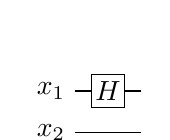
\begin{tikzpicture}[scale=1.000000,x=1pt,y=1pt]
\filldraw[color=white] (0.000000, -7.500000) rectangle (24.000000, 22.500000);
% Drawing wires
% Line 1: a2 W x_2
\draw[color=black] (0.000000,15.000000) -- (24.000000,15.000000);
\draw[color=black] (0.000000,15.000000) node[left] {$x_1$};
% Line 2: a1 W x_1
\draw[color=black] (0.000000,0.000000) -- (24.000000,0.000000);
\draw[color=black] (0.000000,0.000000) node[left] {$x_2$};
% Done with wires; drawing gates
% Line 3: a2 H
\begin{scope}
\draw[fill=white] (12.000000, 15.000000) +(-45.000000:8.485281pt and 8.485281pt) -- +(45.000000:8.485281pt and 8.485281pt) -- +(135.000000:8.485281pt and 8.485281pt) -- +(225.000000:8.485281pt and 8.485281pt) -- cycle;
\clip (12.000000, 15.000000) +(-45.000000:8.485281pt and 8.485281pt) -- +(45.000000:8.485281pt and 8.485281pt) -- +(135.000000:8.485281pt and 8.485281pt) -- +(225.000000:8.485281pt and 8.485281pt) -- cycle;
\draw (12.000000, 15.000000) node {$H$};
\end{scope}
% Done with gates; drawing ending labels
% Done with ending labels; drawing cut lines and comments
% Done with comments
\end{tikzpicture}
\end{center}
in the computation basis?  What is the unitary matrix for the circuit
\begin{center}
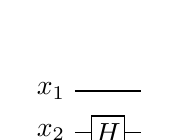
\begin{tikzpicture}[scale=1.000000,x=1pt,y=1pt]
\filldraw[color=white] (0.000000, -7.500000) rectangle (24.000000, 22.500000);
% Drawing wires
% Line 1: a2 W x_2
\draw[color=black] (0.000000,15.000000) -- (24.000000,15.000000);
\draw[color=black] (0.000000,15.000000) node[left] {$x_1$};
% Line 2: a1 W x_1
\draw[color=black] (0.000000,0.000000) -- (24.000000,0.000000);
\draw[color=black] (0.000000,0.000000) node[left] {$x_2$};
% Done with wires; drawing gates
% Line 3: a1 H
\begin{scope}
\draw[fill=white] (12.000000, -0.000000) +(-45.000000:8.485281pt and 8.485281pt) -- +(45.000000:8.485281pt and 8.485281pt) -- +(135.000000:8.485281pt and 8.485281pt) -- +(225.000000:8.485281pt and 8.485281pt) -- cycle;
\clip (12.000000, -0.000000) +(-45.000000:8.485281pt and 8.485281pt) -- +(45.000000:8.485281pt and 8.485281pt) -- +(135.000000:8.485281pt and 8.485281pt) -- +(225.000000:8.485281pt and 8.485281pt) -- cycle;
\draw (12.000000, -0.000000) node {$H$};
\end{scope}
% Done with gates; drawing ending labels
% Done with ending labels; drawing cut lines and comments
% Done with comments
\end{tikzpicture}
\end{center}
in the computational basis?
\Soln Note: we've changed the qubit labels so that reading states top to bottom corresponds to reading them left to right in the concatenated computation basis representation.   The unitary matrices are: $\frac{1}{\sqrt{2}}\begin{bmatrix} 1 & 0 & 1 & 0 \\ 0 & 1 & 0 & 1 \\ 1 & 0 & -1 & 0 \\ 0 & 1 & 0 & -1\end{bmatrix}$ and $\frac{1}{\sqrt{2}}\begin{bmatrix} 1 & 1 & 0 & 0 \\ 1 & -1 & 0 & 0 \\ 0 & 0 & 1 & 1 \\ 0 & 0 & 1 & -1\end{bmatrix}$.

\Textbf{4.17} \textbf{(Building} \CNOT \textbf{\ from controlled-$Z$ gates)} Construct a \CNOT\ gate from one controled-$Z$ gate, that is, the gate whose action in the computational basis is specified by the unitary matrix $$\begin{bmatrix} 1 & 0 & 0 &0 \\ 0 & 1 & 0 & 0 \\ 0 & 0 & 1 & 0 \\ 0 & 0 & 0 & -1\end{bmatrix},$$ and two Hadamard gates, specifying the control and target qubits. 
\Soln The Hadamard gate maps the eigenvectors of the $X$ operator to those of the $Z$ operator, so applying a Hadamard to the control before and after executing a controlled-$Z$ should effect a \CNOT.  
\begin{center}
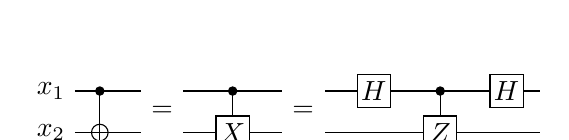
\begin{tikzpicture}[scale=1.000000,x=1pt,y=1pt]
\filldraw[color=white] (0.000000, -7.500000) rectangle (168.000000, 22.500000);
% Drawing wires
% Line 1: a2 W x_2
\draw[color=black] (0.000000,15.000000) -- (168.000000,15.000000);
\draw[color=black] (0.000000,15.000000) node[left] {$x_1$};
% Line 2: a1 W x_1
\draw[color=black] (0.000000,0.000000) -- (168.000000,0.000000);
\draw[color=black] (0.000000,0.000000) node[left] {$x_2$};
% Done with wires; drawing gates
% Line 3: +a1 a2
\draw (9.000000,15.000000) -- (9.000000,0.000000);
\begin{scope}
\draw[fill=white] (9.000000, 0.000000) circle(3.000000pt);
\clip (9.000000, 0.000000) circle(3.000000pt);
\draw (6.000000, 0.000000) -- (12.000000, 0.000000);
\draw (9.000000, -3.000000) -- (9.000000, 3.000000);
\end{scope}
\filldraw (9.000000, 15.000000) circle(1.500000pt);
% Line 4: =
\draw[fill=white,color=white] (24.000000, -6.000000) rectangle (39.000000, 21.000000);
\draw (31.500000, 7.500000) node {$=$};
% Line 5: a1 X a2
\draw (57.000000,15.000000) -- (57.000000,0.000000);
\begin{scope}
\draw[fill=white] (57.000000, -0.000000) +(-45.000000:8.485281pt and 8.485281pt) -- +(45.000000:8.485281pt and 8.485281pt) -- +(135.000000:8.485281pt and 8.485281pt) -- +(225.000000:8.485281pt and 8.485281pt) -- cycle;
\clip (57.000000, -0.000000) +(-45.000000:8.485281pt and 8.485281pt) -- +(45.000000:8.485281pt and 8.485281pt) -- +(135.000000:8.485281pt and 8.485281pt) -- +(225.000000:8.485281pt and 8.485281pt) -- cycle;
\draw (57.000000, -0.000000) node {$X$};
\end{scope}
\filldraw (57.000000, 15.000000) circle(1.500000pt);
% Line 6: =
\draw[fill=white,color=white] (75.000000, -6.000000) rectangle (90.000000, 21.000000);
\draw (82.500000, 7.500000) node {$=$};
% Line 7: a2 H
\begin{scope}
\draw[fill=white] (108.000000, 15.000000) +(-45.000000:8.485281pt and 8.485281pt) -- +(45.000000:8.485281pt and 8.485281pt) -- +(135.000000:8.485281pt and 8.485281pt) -- +(225.000000:8.485281pt and 8.485281pt) -- cycle;
\clip (108.000000, 15.000000) +(-45.000000:8.485281pt and 8.485281pt) -- +(45.000000:8.485281pt and 8.485281pt) -- +(135.000000:8.485281pt and 8.485281pt) -- +(225.000000:8.485281pt and 8.485281pt) -- cycle;
\draw (108.000000, 15.000000) node {$H$};
\end{scope}
% Line 8: a1 Z a2
\draw (132.000000,15.000000) -- (132.000000,0.000000);
\begin{scope}
\draw[fill=white] (132.000000, -0.000000) +(-45.000000:8.485281pt and 8.485281pt) -- +(45.000000:8.485281pt and 8.485281pt) -- +(135.000000:8.485281pt and 8.485281pt) -- +(225.000000:8.485281pt and 8.485281pt) -- cycle;
\clip (132.000000, -0.000000) +(-45.000000:8.485281pt and 8.485281pt) -- +(45.000000:8.485281pt and 8.485281pt) -- +(135.000000:8.485281pt and 8.485281pt) -- +(225.000000:8.485281pt and 8.485281pt) -- cycle;
\draw (132.000000, -0.000000) node {$Z$};
\end{scope}
\filldraw (132.000000, 15.000000) circle(1.500000pt);
% Line 9: a2 H
\begin{scope}
\draw[fill=white] (156.000000, 15.000000) +(-45.000000:8.485281pt and 8.485281pt) -- +(45.000000:8.485281pt and 8.485281pt) -- +(135.000000:8.485281pt and 8.485281pt) -- +(225.000000:8.485281pt and 8.485281pt) -- cycle;
\clip (156.000000, 15.000000) +(-45.000000:8.485281pt and 8.485281pt) -- +(45.000000:8.485281pt and 8.485281pt) -- +(135.000000:8.485281pt and 8.485281pt) -- +(225.000000:8.485281pt and 8.485281pt) -- cycle;
\draw (156.000000, 15.000000) node {$H$};
\end{scope}
% Done with gates; drawing ending labels
% Done with ending labels; drawing cut lines and comments
% Done with comments
\end{tikzpicture}
\end{center}
In matrix form, this corresponds to $$\begin{bmatrix} 1 & 0 & 0 & 0 \\ 0 & 1 & 0 & 0 \\ 0 & 0 & 0 & 1 \\ 0 & 0 & 1 & 0 \end{bmatrix} = \frac{1}{2}\begin{bmatrix} 1 & 0 & 1 & 0 \\ 0 & 1 & 0 & 1 \\ 1 & 0 & -1 & 0 \\ 0 & 1 & 0 & -1\end{bmatrix}\begin{bmatrix} 1 & 0 & 0 &0 \\ 0 & 1 & 0 & 0 \\ 0 & 0 & 1 & 0 \\ 0 & 0 & 0 & -1\end{bmatrix}\begin{bmatrix} 1 & 0 & 1 & 0 \\ 0 & 1 & 0 & 1 \\ 1 & 0 & -1 & 0 \\ 0 & 1 & 0 & -1\end{bmatrix}.$$

\Textbf{4.18} Show that 
\begin{center}
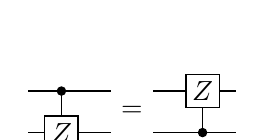
\begin{tikzpicture}[scale=1.000000,x=1pt,y=1pt]
\filldraw[color=white] (0.000000, -7.500000) rectangle (75.000000, 22.500000);
% Drawing wires
% Line 1: a2 W
\draw[color=black] (0.000000,15.000000) -- (75.000000,15.000000);
% Line 2: a1 W
\draw[color=black] (0.000000,0.000000) -- (75.000000,0.000000);
% Done with wires; drawing gates
% Line 3: a1 Z a2
\draw (12.000000,15.000000) -- (12.000000,0.000000);
\begin{scope}
\draw[fill=white] (12.000000, -0.000000) +(-45.000000:8.485281pt and 8.485281pt) -- +(45.000000:8.485281pt and 8.485281pt) -- +(135.000000:8.485281pt and 8.485281pt) -- +(225.000000:8.485281pt and 8.485281pt) -- cycle;
\clip (12.000000, -0.000000) +(-45.000000:8.485281pt and 8.485281pt) -- +(45.000000:8.485281pt and 8.485281pt) -- +(135.000000:8.485281pt and 8.485281pt) -- +(225.000000:8.485281pt and 8.485281pt) -- cycle;
\draw (12.000000, -0.000000) node {$Z$};
\end{scope}
\filldraw (12.000000, 15.000000) circle(1.500000pt);
% Line 4: =
\draw[fill=white,color=white] (30.000000, -6.000000) rectangle (45.000000, 21.000000);
\draw (37.500000, 7.500000) node {$=$};
% Line 5: a2 Z a1
\draw (63.000000,15.000000) -- (63.000000,0.000000);
\begin{scope}
\draw[fill=white] (63.000000, 15.000000) +(-45.000000:8.485281pt and 8.485281pt) -- +(45.000000:8.485281pt and 8.485281pt) -- +(135.000000:8.485281pt and 8.485281pt) -- +(225.000000:8.485281pt and 8.485281pt) -- cycle;
\clip (63.000000, 15.000000) +(-45.000000:8.485281pt and 8.485281pt) -- +(45.000000:8.485281pt and 8.485281pt) -- +(135.000000:8.485281pt and 8.485281pt) -- +(225.000000:8.485281pt and 8.485281pt) -- cycle;
\draw (63.000000, 15.000000) node {$Z$};
\end{scope}
\filldraw (63.000000, 0.000000) circle(1.500000pt);
% Done with gates; drawing ending labels
% Done with ending labels; drawing cut lines and comments
% Done with comments
\end{tikzpicture}
\end{center}
\Soln In the computational basis the controlled-$Z$ changes the state if and only if the control and target qubits are both $\ket{1}$.  In this criteria the control and target are interchangeable, so these gates perform the same action.
\newpage
\Textbf{4.19} \textbf{(}\CNOT\ \textbf{action on density matrices)} The \CNOT\ gate is a simple permutation whose action on a density matrix $\rho$ is to rearrange the elements in the matrix. Write out this action explicitly in the computational basis.
\Soln $$\ket{x_2x_1} = \alpha\ket{00}+\beta\ket{01}+\gamma\ket{10}+\delta\ket{11} \xrightarrow[]{CX} \alpha\ket{00}+\beta\ket{01}+\underline{\delta}\ket{10}+\underline{\gamma}\ket{11}.$$

\Textbf{4.20} \textbf{(}\CNOT\ \textbf{basis transformation)} Unlike ideal classical gates, ideal quantum gates do not have (as electrical engineers say) `high-impedence' inputs.  In fact, the role of `control' and `target' are arbitrary -- they depend on what basis you think of a device as operating in.  We have described how the \CNOT\ behaves with respect to the computational basis, and in this description the state of the control qubit is not changed.  However, if we work in a different basis then the control qubit \textit{does} change: we will show that its phase is flipped depending on the state of the `target' qubit!  Show that
\begin{center}
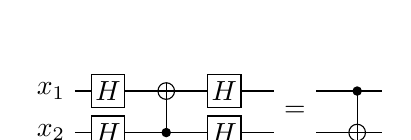
\begin{tikzpicture}[scale=1.000000,x=1pt,y=1pt]
\filldraw[color=white] (0.000000, -7.500000) rectangle (111.000000, 22.500000);
% Drawing wires
% Line 1: a1 W $x_1$
\draw[color=black] (0.000000,15.000000) -- (111.000000,15.000000);
\draw[color=black] (0.000000,15.000000) node[left] {$x_1$};
% Line 2: a2 W $x_2$
\draw[color=black] (0.000000,0.000000) -- (111.000000,0.000000);
\draw[color=black] (0.000000,0.000000) node[left] {$x_2$};
% Done with wires; drawing gates
% Line 3: a1 H
\begin{scope}
\draw[fill=white] (12.000000, 15.000000) +(-45.000000:8.485281pt and 8.485281pt) -- +(45.000000:8.485281pt and 8.485281pt) -- +(135.000000:8.485281pt and 8.485281pt) -- +(225.000000:8.485281pt and 8.485281pt) -- cycle;
\clip (12.000000, 15.000000) +(-45.000000:8.485281pt and 8.485281pt) -- +(45.000000:8.485281pt and 8.485281pt) -- +(135.000000:8.485281pt and 8.485281pt) -- +(225.000000:8.485281pt and 8.485281pt) -- cycle;
\draw (12.000000, 15.000000) node {$H$};
\end{scope}
% Line 4: a2 H
\begin{scope}
\draw[fill=white] (12.000000, -0.000000) +(-45.000000:8.485281pt and 8.485281pt) -- +(45.000000:8.485281pt and 8.485281pt) -- +(135.000000:8.485281pt and 8.485281pt) -- +(225.000000:8.485281pt and 8.485281pt) -- cycle;
\clip (12.000000, -0.000000) +(-45.000000:8.485281pt and 8.485281pt) -- +(45.000000:8.485281pt and 8.485281pt) -- +(135.000000:8.485281pt and 8.485281pt) -- +(225.000000:8.485281pt and 8.485281pt) -- cycle;
\draw (12.000000, -0.000000) node {$H$};
\end{scope}
% Line 5: +a1 a2
\draw (33.000000,15.000000) -- (33.000000,0.000000);
\begin{scope}
\draw[fill=white] (33.000000, 15.000000) circle(3.000000pt);
\clip (33.000000, 15.000000) circle(3.000000pt);
\draw (30.000000, 15.000000) -- (36.000000, 15.000000);
\draw (33.000000, 12.000000) -- (33.000000, 18.000000);
\end{scope}
\filldraw (33.000000, 0.000000) circle(1.500000pt);
% Line 6: a1 H
\begin{scope}
\draw[fill=white] (54.000000, 15.000000) +(-45.000000:8.485281pt and 8.485281pt) -- +(45.000000:8.485281pt and 8.485281pt) -- +(135.000000:8.485281pt and 8.485281pt) -- +(225.000000:8.485281pt and 8.485281pt) -- cycle;
\clip (54.000000, 15.000000) +(-45.000000:8.485281pt and 8.485281pt) -- +(45.000000:8.485281pt and 8.485281pt) -- +(135.000000:8.485281pt and 8.485281pt) -- +(225.000000:8.485281pt and 8.485281pt) -- cycle;
\draw (54.000000, 15.000000) node {$H$};
\end{scope}
% Line 7: a2 H
\begin{scope}
\draw[fill=white] (54.000000, -0.000000) +(-45.000000:8.485281pt and 8.485281pt) -- +(45.000000:8.485281pt and 8.485281pt) -- +(135.000000:8.485281pt and 8.485281pt) -- +(225.000000:8.485281pt and 8.485281pt) -- cycle;
\clip (54.000000, -0.000000) +(-45.000000:8.485281pt and 8.485281pt) -- +(45.000000:8.485281pt and 8.485281pt) -- +(135.000000:8.485281pt and 8.485281pt) -- +(225.000000:8.485281pt and 8.485281pt) -- cycle;
\draw (54.000000, -0.000000) node {$H$};
\end{scope}
% Line 8: =
\draw[fill=white,color=white] (72.000000, -6.000000) rectangle (87.000000, 21.000000);
\draw (79.500000, 7.500000) node {$=$};
% Line 9: a1 +a2
\draw (102.000000,15.000000) -- (102.000000,0.000000);
\filldraw (102.000000, 15.000000) circle(1.500000pt);
\begin{scope}
\draw[fill=white] (102.000000, 0.000000) circle(3.000000pt);
\clip (102.000000, 0.000000) circle(3.000000pt);
\draw (99.000000, 0.000000) -- (105.000000, 0.000000);
\draw (102.000000, -3.000000) -- (102.000000, 3.000000);
\end{scope}
% Done with gates; drawing ending labels
% Done with ending labels; drawing cut lines and comments
% Done with comments
\end{tikzpicture}
\end{center}
Introducing basis states $\ket{\pm}\equiv(\ket{0}\pm\ket{1})/\sqrt{2}$, use this circuit identity to show that the effect of a \CNOT\ with the first qubit as control and the second qubit as target is as follows:
\begin{align*}
\ket{x_1}\ket{x_2}& \\
\ket{+}\ket{+}&\rightarrow\ket{+}\ket{+}\\
\ket{-}\ket{+}&\rightarrow\ket{-}\ket{+}\\
\ket{+}\ket{-}&\rightarrow\ket{-}\ket{-}\\
\ket{-}\ket{-}&\rightarrow\ket{+}\ket{-}.
\end{align*}
Thus, with respect to the this new basis, the state of the target qubit is not changed, while the state of the control qubit is flipped if the target starts as $\ket{-}$, otherwise it is left alone. That is, in this basis, the target and control have essentially interchanged roles!
\Soln Note, we've switched the roles of qubits in the diagram (and labeled them)  so that reading states top to bottom in the diagram corresponds to reading them left to right in the concatenated basis representation.  To show the circuit identity, we use matrix multiplication:
$$\frac{1}{4} \begin{bmatrix} 1 & 1 & 0 & 0 \\ 1 & -1 & 0 & 0 \\ 0 & 0 & 1 & 1 \\ 0 & 0 & 1 & -1\end{bmatrix}\begin{bmatrix} 1 & 0 & 1 & 0 \\ 0 & 1 & 0 & 1 \\ 1 & 0 & -1 & 0 \\ 0 & 1 & 0 & -1\end{bmatrix} \begin{bmatrix} 1 & 0 & 0 &0 \\ 0 & 0 & 0 & 1 \\ 0 & 0 & 1 & 0 \\ 0 & 1 & 0 & 0\end{bmatrix}\begin{bmatrix} 1 & 1 & 0 & 0 \\ 1 & -1 & 0 & 0 \\ 0 & 0 & 1 & 1 \\ 0 & 0 & 1 & -1\end{bmatrix}\begin{bmatrix} 1 & 0 & 1 & 0 \\ 0 & 1 & 0 & 1 \\ 1 & 0 & -1 & 0 \\ 0 & 1 & 0 & -1\end{bmatrix} =\begin{bmatrix} 1 & 0 & 0 &0 \\ 0 & 1 & 0 & 0 \\ 0 & 0 & 0 & 1 \\ 0 & 0 & 1 & 0\end{bmatrix}.$$
\vspace{-15pt}
\begin{center}\ \ \ \ $H(x_1,\_)$ \quad\quad\quad\quad $H(\_, x_2)$  \quad\quad \CNOT$(x_2,x_1)$ \quad\quad $H(x_1,\_)$ \quad\quad\quad $H(\_, x_2)$ \quad\quad\quad \CNOT$(x_1,x_2)$ \end{center}
The matrix in the middle on the left can be verified to be the representation of the action of \CNOT\ in the computational basis, with $x_2$ as control, and $x_1$  as target.  In functional notation below, we'll let \CNOT$(x_1, x_2)$ denote the action of a \CNOT\ controlled by $\ket{x_1}$ and targetting $\ket{x_2}$, with \CNOT$'(x_1,x_2) \equiv$ \CNOT$(x_2,x_1)$ switching target and control, and let $H(x_1, x_2)$ denote the application of Hadamard gates to both qubits.  The circuit identity is that $H($\CNOT$'(H(x_1, x_2)) =\ $\CNOT$(x_1,x_2)$.  Now:

\begin{center}
\textcolor{white}{\CNOT}$(\ket{x_1},\ket{x_2})$\textcolor{white}{$ = H($\CNOT$''(H(\ket{+},\ket{+}))) = H($\CNOT$'(\ket{0},\ket{0})) = H(\ket{0},\ket{0}) = \ket{+}\ket{+}$}
\CNOT$(\ket{+},\ket{+}) = H($\CNOT$'(H(\ket{+},\ket{+}))) = H($\CNOT$'(\ket{0},\ket{0})) = H(\ket{0},\ket{0}) = \ket{+}\ket{+}$
\CNOT$(\ket{-},\ket{+}) = H($\CNOT$'(H(\ket{-},\ket{+}))) = H($\CNOT$'(\ket{1},\ket{0})) = H(\ket{1},\ket{0}) = \ket{-}\ket{+}$ % This isn't right, I can't keep track of the endianess
\CNOT$(\ket{+},\ket{-}) = H($\CNOT$'(H(\ket{+},\ket{-}))) = H($\CNOT$'(\ket{0},\ket{1})) = H(\ket{1},\ket{1}) = \ket{-}\ket{-}$
\CNOT$(\ket{-},\ket{-}) = H($\CNOT$'(H(\ket{-},\ket{-}))) = H($\CNOT$'(\ket{1},\ket{1})) = H(\ket{0},\ket{1}) = \ket{+}\ket{-}$ % This isn't right, I can't keep track of the endianess
\end{center}
\Textbf{4.21} Suppose $U$ is a single qubit unitary operator, and $V$ is a unitary operator chosen so that $V^2=U$.  Verify that Figure 4.8 implements the $C^2(U)$ operation.
\begin{center}
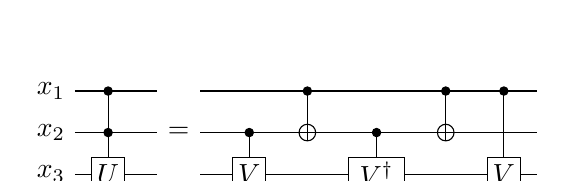
\begin{tikzpicture}[scale=1.000000,x=1pt,y=1pt]
\filldraw[color=white] (0.000000, -7.500000) rectangle (167.000000, 37.500000);
% Drawing wires
% Line 1: a3 W x_3
\draw[color=black] (0.000000,30.000000) -- (167.000000,30.000000);
\draw[color=black] (0.000000,30.000000) node[left] {$x_1$};
% Line 2: a2 W x_2
\draw[color=black] (0.000000,15.000000) -- (167.000000,15.000000);
\draw[color=black] (0.000000,15.000000) node[left] {$x_2$};
% Line 3: a1 W x_1
\draw[color=black] (0.000000,0.000000) -- (167.000000,0.000000);
\draw[color=black] (0.000000,0.000000) node[left] {$x_3$};
% Done with wires; drawing gates
% Line 4: a1 G $U$ a2 a3
\draw (12.000000,30.000000) -- (12.000000,0.000000);
\begin{scope}
\draw[fill=white] (12.000000, -0.000000) +(-45.000000:8.485281pt and 8.485281pt) -- +(45.000000:8.485281pt and 8.485281pt) -- +(135.000000:8.485281pt and 8.485281pt) -- +(225.000000:8.485281pt and 8.485281pt) -- cycle;
\clip (12.000000, -0.000000) +(-45.000000:8.485281pt and 8.485281pt) -- +(45.000000:8.485281pt and 8.485281pt) -- +(135.000000:8.485281pt and 8.485281pt) -- +(225.000000:8.485281pt and 8.485281pt) -- cycle;
\draw (12.000000, -0.000000) node {$U$};
\end{scope}
\filldraw (12.000000, 15.000000) circle(1.500000pt);
\filldraw (12.000000, 30.000000) circle(1.500000pt);
% Line 5: =
\draw[fill=white,color=white] (30.000000, -6.000000) rectangle (45.000000, 36.000000);
\draw (37.500000, 15.000000) node {$=$};
% Line 6: a1 G $V$ a2
\draw (63.000000,15.000000) -- (63.000000,0.000000);
\begin{scope}
\draw[fill=white] (63.000000, -0.000000) +(-45.000000:8.485281pt and 8.485281pt) -- +(45.000000:8.485281pt and 8.485281pt) -- +(135.000000:8.485281pt and 8.485281pt) -- +(225.000000:8.485281pt and 8.485281pt) -- cycle;
\clip (63.000000, -0.000000) +(-45.000000:8.485281pt and 8.485281pt) -- +(45.000000:8.485281pt and 8.485281pt) -- +(135.000000:8.485281pt and 8.485281pt) -- +(225.000000:8.485281pt and 8.485281pt) -- cycle;
\draw (63.000000, -0.000000) node {$V$};
\end{scope}
\filldraw (63.000000, 15.000000) circle(1.500000pt);
% Line 7: +a2 a3
\draw (84.000000,30.000000) -- (84.000000,15.000000);
\begin{scope}
\draw[fill=white] (84.000000, 15.000000) circle(3.000000pt);
\clip (84.000000, 15.000000) circle(3.000000pt);
\draw (81.000000, 15.000000) -- (87.000000, 15.000000);
\draw (84.000000, 12.000000) -- (84.000000, 18.000000);
\end{scope}
\filldraw (84.000000, 30.000000) circle(1.500000pt);
% Line 8: a1 G $V^\dagger$ a2 width=20
\draw (109.000000,15.000000) -- (109.000000,0.000000);
\begin{scope}
\draw[fill=white] (109.000000, -0.000000) +(-45.000000:14.142136pt and 8.485281pt) -- +(45.000000:14.142136pt and 8.485281pt) -- +(135.000000:14.142136pt and 8.485281pt) -- +(225.000000:14.142136pt and 8.485281pt) -- cycle;
\clip (109.000000, -0.000000) +(-45.000000:14.142136pt and 8.485281pt) -- +(45.000000:14.142136pt and 8.485281pt) -- +(135.000000:14.142136pt and 8.485281pt) -- +(225.000000:14.142136pt and 8.485281pt) -- cycle;
\draw (109.000000, -0.000000) node {$V^\dagger$};
\end{scope}
\filldraw (109.000000, 15.000000) circle(1.500000pt);
% Line 9: +a2 a3
\draw (134.000000,30.000000) -- (134.000000,15.000000);
\begin{scope}
\draw[fill=white] (134.000000, 15.000000) circle(3.000000pt);
\clip (134.000000, 15.000000) circle(3.000000pt);
\draw (131.000000, 15.000000) -- (137.000000, 15.000000);
\draw (134.000000, 12.000000) -- (134.000000, 18.000000);
\end{scope}
\filldraw (134.000000, 30.000000) circle(1.500000pt);
% Line 10: a1 G $V$ a3
\draw (155.000000,30.000000) -- (155.000000,0.000000);
\begin{scope}
\draw[fill=white] (155.000000, -0.000000) +(-45.000000:8.485281pt and 8.485281pt) -- +(45.000000:8.485281pt and 8.485281pt) -- +(135.000000:8.485281pt and 8.485281pt) -- +(225.000000:8.485281pt and 8.485281pt) -- cycle;
\clip (155.000000, -0.000000) +(-45.000000:8.485281pt and 8.485281pt) -- +(45.000000:8.485281pt and 8.485281pt) -- +(135.000000:8.485281pt and 8.485281pt) -- +(225.000000:8.485281pt and 8.485281pt) -- cycle;
\draw (155.000000, -0.000000) node {$V$};
\end{scope}
\filldraw (155.000000, 30.000000) circle(1.500000pt);
% Done with gates; drawing ending labels
% Done with ending labels; drawing cut lines and comments
% Done with comments
\end{tikzpicture}
\end{center}
\vspace{-15pt}
\Soln We verify by tracking the applications of $V$ and $V^\dagger$ to $\ket{x_3}$ for each computational basis state representing $\ket{x_1}\ket{x_2}$.  The first $V$ is applied when $\ket{x_2}=\ket{1}$.  The first \CNOT\ calculates the parity of $\ket{x_1}\ket{x_2}$ so that the middle $V^\dagger$ is applied for when $\ket{x_1}\ket{x_2} = \ket{0}\ket{1}\ \mathrm{or}\ \ket{1}\ket{0}$.  The second \CNOT\ uncomputes the parity  so that in the end $\ket{x_1}\ket{x_2}$ is unchanged.  The final $V$ is then applied if $\ket{x_1}=\ket{1}$.  In the end, the output of the circuit is
\begin{align*}
\ket{x_1}\ket{x_2}\ \ \ \ \\
\ket{0}\ket{0}\ket{x_3}\ &\rightarrow \ket{0}\ket{0}\ \ \ \ \ \ \ \ket{x_3} \\
\ket{0}\ket{1}\ket{x_3}\ &\rightarrow\ket{0}\ket{1}VV^\dagger\ket{x_3} =\ket{0}\ket{1}\ \ \ \ket{x_3} \tag{$V$ is unitary, $VV^\dagger=I$}\\
\ket{1}\ket{0}\ket{x_3}\ &\rightarrow\ket{1}\ket{0} V^\dagger V\ket{x_3} = \ket{1}\ket{0}\ \ \ \ket{x_3} \tag{$V$ is unitary, $V^\dagger V=I$}\\
\ket{1}\ket{1}\ket{x_3}\ &\rightarrow \ket{1}\ket{1}\ \ V^2\ket{x_3}=\ket{1}\ket{1} U\ket{x_3} \tag{$   V^2=U$}
\end{align*}

\Textbf{4.22} Prove that a $C^2(U)$ gate (for any single qubit unitary $U$) can be constructed using at most eight one-qubit gates, and six controlled-\NOT s
\Soln Note: this solution borrows heavily from  DaftWullie's answer to the quantumcomputing.stackexhange question here: \href{_}\url{https://quantumcomputing.stackexchange.com/questions/7082/how-to-reduce-circuit-elements-of-a-decomposed-c2u-operation}.

 Let $V$ be a single-qubit unitary operator such that $V^2=U$, and By Corollary 4.2, let $A,B,$ and $C$ be single-qubit unitary operators and $\alpha$ an overall phase factor such that $ABC=I$ and $V=e^{i\alpha}AXBXC$. Combining figures 4.6 and 4.8 gives

\begin{center}
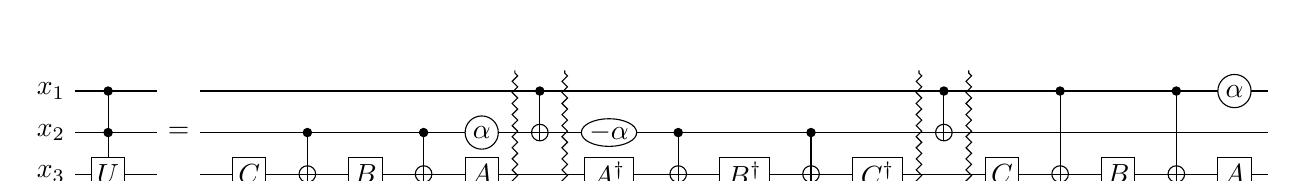
\begin{tikzpicture}[scale=1.000000,x=1pt,y=1pt]
\filldraw[color=white] (0.000000, -7.500000) rectangle (431.000000, 37.500000);
% Drawing wires
% Line 1: a3 W x_3
\draw[color=black] (0.000000,30.000000) -- (431.000000,30.000000);
\draw[color=black] (0.000000,30.000000) node[left] {$x_1$};
% Line 2: a2 W x_2
\draw[color=black] (0.000000,15.000000) -- (431.000000,15.000000);
\draw[color=black] (0.000000,15.000000) node[left] {$x_2$};
% Line 3: a1 W x_1
\draw[color=black] (0.000000,0.000000) -- (431.000000,0.000000);
\draw[color=black] (0.000000,0.000000) node[left] {$x_3$};
% Done with wires; drawing gates
% Line 4: a1 G $U$ a2 a3
\draw (12.000000,30.000000) -- (12.000000,0.000000);
\begin{scope}
\draw[fill=white] (12.000000, -0.000000) +(-45.000000:8.485281pt and 8.485281pt) -- +(45.000000:8.485281pt and 8.485281pt) -- +(135.000000:8.485281pt and 8.485281pt) -- +(225.000000:8.485281pt and 8.485281pt) -- cycle;
\clip (12.000000, -0.000000) +(-45.000000:8.485281pt and 8.485281pt) -- +(45.000000:8.485281pt and 8.485281pt) -- +(135.000000:8.485281pt and 8.485281pt) -- +(225.000000:8.485281pt and 8.485281pt) -- cycle;
\draw (12.000000, -0.000000) node {$U$};
\end{scope}
\filldraw (12.000000, 15.000000) circle(1.500000pt);
\filldraw (12.000000, 30.000000) circle(1.500000pt);
% Line 5: =
\draw[fill=white,color=white] (30.000000, -6.000000) rectangle (45.000000, 36.000000);
\draw (37.500000, 15.000000) node {$=$};
% Line 6: a1 G $C$
\begin{scope}
\draw[fill=white] (63.000000, -0.000000) +(-45.000000:8.485281pt and 8.485281pt) -- +(45.000000:8.485281pt and 8.485281pt) -- +(135.000000:8.485281pt and 8.485281pt) -- +(225.000000:8.485281pt and 8.485281pt) -- cycle;
\clip (63.000000, -0.000000) +(-45.000000:8.485281pt and 8.485281pt) -- +(45.000000:8.485281pt and 8.485281pt) -- +(135.000000:8.485281pt and 8.485281pt) -- +(225.000000:8.485281pt and 8.485281pt) -- cycle;
\draw (63.000000, -0.000000) node {$C$};
\end{scope}
% Line 7: +a1 a2
\draw (84.000000,15.000000) -- (84.000000,0.000000);
\begin{scope}
\draw[fill=white] (84.000000, 0.000000) circle(3.000000pt);
\clip (84.000000, 0.000000) circle(3.000000pt);
\draw (81.000000, 0.000000) -- (87.000000, 0.000000);
\draw (84.000000, -3.000000) -- (84.000000, 3.000000);
\end{scope}
\filldraw (84.000000, 15.000000) circle(1.500000pt);
% Line 8: a1 G $B$
\begin{scope}
\draw[fill=white] (105.000000, -0.000000) +(-45.000000:8.485281pt and 8.485281pt) -- +(45.000000:8.485281pt and 8.485281pt) -- +(135.000000:8.485281pt and 8.485281pt) -- +(225.000000:8.485281pt and 8.485281pt) -- cycle;
\clip (105.000000, -0.000000) +(-45.000000:8.485281pt and 8.485281pt) -- +(45.000000:8.485281pt and 8.485281pt) -- +(135.000000:8.485281pt and 8.485281pt) -- +(225.000000:8.485281pt and 8.485281pt) -- cycle;
\draw (105.000000, -0.000000) node {$B$};
\end{scope}
% Line 9: +a1 a2
\draw (126.000000,15.000000) -- (126.000000,0.000000);
\begin{scope}
\draw[fill=white] (126.000000, 0.000000) circle(3.000000pt);
\clip (126.000000, 0.000000) circle(3.000000pt);
\draw (123.000000, 0.000000) -- (129.000000, 0.000000);
\draw (126.000000, -3.000000) -- (126.000000, 3.000000);
\end{scope}
\filldraw (126.000000, 15.000000) circle(1.500000pt);
% Line 10: a2 P $\alpha$
\begin{scope}
\draw[fill=white] (147.000000, 15.000000) circle(6.000000pt);
\clip (147.000000, 15.000000) circle(6.000000pt);
\draw (147.000000, 15.000000) node {$\alpha$};
\end{scope}
% Line 11: a1 G $A$
\begin{scope}
\draw[fill=white] (147.000000, -0.000000) +(-45.000000:8.485281pt and 8.485281pt) -- +(45.000000:8.485281pt and 8.485281pt) -- +(135.000000:8.485281pt and 8.485281pt) -- +(225.000000:8.485281pt and 8.485281pt) -- cycle;
\clip (147.000000, -0.000000) +(-45.000000:8.485281pt and 8.485281pt) -- +(45.000000:8.485281pt and 8.485281pt) -- +(135.000000:8.485281pt and 8.485281pt) -- +(225.000000:8.485281pt and 8.485281pt) -- cycle;
\draw (147.000000, -0.000000) node {$A$};
\end{scope}
% Line 12: a3 a2 a1 BARRIER
\draw[decorate,decoration={zigzag,amplitude=1pt,segment length=4}] (159.000000,-7.500000) -- (159.000000,37.500000);
% Line 13: +a2 a3
\draw (168.000000,30.000000) -- (168.000000,15.000000);
\begin{scope}
\draw[fill=white] (168.000000, 15.000000) circle(3.000000pt);
\clip (168.000000, 15.000000) circle(3.000000pt);
\draw (165.000000, 15.000000) -- (171.000000, 15.000000);
\draw (168.000000, 12.000000) -- (168.000000, 18.000000);
\end{scope}
\filldraw (168.000000, 30.000000) circle(1.500000pt);
% Line 14: a3 a2 a1 BARRIER
\draw[decorate,decoration={zigzag,amplitude=1pt,segment length=4}] (177.000000,-7.500000) -- (177.000000,37.500000);
% Line 16: a1 G $A^\dagger$ width=18
\begin{scope}
\draw[fill=white] (193.000000, -0.000000) +(-45.000000:12.727922pt and 8.485281pt) -- +(45.000000:12.727922pt and 8.485281pt) -- +(135.000000:12.727922pt and 8.485281pt) -- +(225.000000:12.727922pt and 8.485281pt) -- cycle;
\clip (193.000000, -0.000000) +(-45.000000:12.727922pt and 8.485281pt) -- +(45.000000:12.727922pt and 8.485281pt) -- +(135.000000:12.727922pt and 8.485281pt) -- +(225.000000:12.727922pt and 8.485281pt) -- cycle;
\draw (193.000000, -0.000000) node {$A^\dagger$};
\end{scope}
% Line 17: a2 P $-\alpha$ height=10 width=20
\begin{scope}
\draw[fill=white] (193.000000, 15.000000) ellipse(10.000000pt and 5.000000pt);
\clip (193.000000, 15.000000) ellipse(10.000000pt and 5.000000pt);
\draw (193.000000, 15.000000) node {$-\alpha$};
\end{scope}
% Line 18: +a1 a2
\draw (218.000000,15.000000) -- (218.000000,0.000000);
\begin{scope}
\draw[fill=white] (218.000000, 0.000000) circle(3.000000pt);
\clip (218.000000, 0.000000) circle(3.000000pt);
\draw (215.000000, 0.000000) -- (221.000000, 0.000000);
\draw (218.000000, -3.000000) -- (218.000000, 3.000000);
\end{scope}
\filldraw (218.000000, 15.000000) circle(1.500000pt);
% Line 19: a1 G $B^\dagger$ width=18
\begin{scope}
\draw[fill=white] (242.000000, -0.000000) +(-45.000000:12.727922pt and 8.485281pt) -- +(45.000000:12.727922pt and 8.485281pt) -- +(135.000000:12.727922pt and 8.485281pt) -- +(225.000000:12.727922pt and 8.485281pt) -- cycle;
\clip (242.000000, -0.000000) +(-45.000000:12.727922pt and 8.485281pt) -- +(45.000000:12.727922pt and 8.485281pt) -- +(135.000000:12.727922pt and 8.485281pt) -- +(225.000000:12.727922pt and 8.485281pt) -- cycle;
\draw (242.000000, -0.000000) node {$B^\dagger$};
\end{scope}
% Line 20: +a1 a2
\draw (266.000000,15.000000) -- (266.000000,0.000000);
\begin{scope}
\draw[fill=white] (266.000000, 0.000000) circle(3.000000pt);
\clip (266.000000, 0.000000) circle(3.000000pt);
\draw (263.000000, 0.000000) -- (269.000000, 0.000000);
\draw (266.000000, -3.000000) -- (266.000000, 3.000000);
\end{scope}
\filldraw (266.000000, 15.000000) circle(1.500000pt);
% Line 21: a1 G $C^\dagger$ width=18
\begin{scope}
\draw[fill=white] (290.000000, -0.000000) +(-45.000000:12.727922pt and 8.485281pt) -- +(45.000000:12.727922pt and 8.485281pt) -- +(135.000000:12.727922pt and 8.485281pt) -- +(225.000000:12.727922pt and 8.485281pt) -- cycle;
\clip (290.000000, -0.000000) +(-45.000000:12.727922pt and 8.485281pt) -- +(45.000000:12.727922pt and 8.485281pt) -- +(135.000000:12.727922pt and 8.485281pt) -- +(225.000000:12.727922pt and 8.485281pt) -- cycle;
\draw (290.000000, -0.000000) node {$C^\dagger$};
\end{scope}
% Line 22: a3 a2 a1 BARRIER
\draw[decorate,decoration={zigzag,amplitude=1pt,segment length=4}] (305.000000,-7.500000) -- (305.000000,37.500000);
% Line 23: +a2 a3
\draw (314.000000,30.000000) -- (314.000000,15.000000);
\begin{scope}
\draw[fill=white] (314.000000, 15.000000) circle(3.000000pt);
\clip (314.000000, 15.000000) circle(3.000000pt);
\draw (311.000000, 15.000000) -- (317.000000, 15.000000);
\draw (314.000000, 12.000000) -- (314.000000, 18.000000);
\end{scope}
\filldraw (314.000000, 30.000000) circle(1.500000pt);
% Line 24: a3 a2 a1 BARRIER
\draw[decorate,decoration={zigzag,amplitude=1pt,segment length=4}] (323.000000,-7.500000) -- (323.000000,37.500000);
% Line 25: a1 G $C$
\begin{scope}
\draw[fill=white] (335.000000, -0.000000) +(-45.000000:8.485281pt and 8.485281pt) -- +(45.000000:8.485281pt and 8.485281pt) -- +(135.000000:8.485281pt and 8.485281pt) -- +(225.000000:8.485281pt and 8.485281pt) -- cycle;
\clip (335.000000, -0.000000) +(-45.000000:8.485281pt and 8.485281pt) -- +(45.000000:8.485281pt and 8.485281pt) -- +(135.000000:8.485281pt and 8.485281pt) -- +(225.000000:8.485281pt and 8.485281pt) -- cycle;
\draw (335.000000, -0.000000) node {$C$};
\end{scope}
% Line 26: +a1 a3
\draw (356.000000,30.000000) -- (356.000000,0.000000);
\begin{scope}
\draw[fill=white] (356.000000, 0.000000) circle(3.000000pt);
\clip (356.000000, 0.000000) circle(3.000000pt);
\draw (353.000000, 0.000000) -- (359.000000, 0.000000);
\draw (356.000000, -3.000000) -- (356.000000, 3.000000);
\end{scope}
\filldraw (356.000000, 30.000000) circle(1.500000pt);
% Line 27: a1 G $B$
\begin{scope}
\draw[fill=white] (377.000000, -0.000000) +(-45.000000:8.485281pt and 8.485281pt) -- +(45.000000:8.485281pt and 8.485281pt) -- +(135.000000:8.485281pt and 8.485281pt) -- +(225.000000:8.485281pt and 8.485281pt) -- cycle;
\clip (377.000000, -0.000000) +(-45.000000:8.485281pt and 8.485281pt) -- +(45.000000:8.485281pt and 8.485281pt) -- +(135.000000:8.485281pt and 8.485281pt) -- +(225.000000:8.485281pt and 8.485281pt) -- cycle;
\draw (377.000000, -0.000000) node {$B$};
\end{scope}
% Line 28: +a1 a3
\draw (398.000000,30.000000) -- (398.000000,0.000000);
\begin{scope}
\draw[fill=white] (398.000000, 0.000000) circle(3.000000pt);
\clip (398.000000, 0.000000) circle(3.000000pt);
\draw (395.000000, 0.000000) -- (401.000000, 0.000000);
\draw (398.000000, -3.000000) -- (398.000000, 3.000000);
\end{scope}
\filldraw (398.000000, 30.000000) circle(1.500000pt);
% Line 29: a3 P $\alpha$
\begin{scope}
\draw[fill=white] (419.000000, 30.000000) circle(6.000000pt);
\clip (419.000000, 30.000000) circle(6.000000pt);
\draw (419.000000, 30.000000) node {$\alpha$};
\end{scope}
% Line 30: a1 G $A$
\begin{scope}
\draw[fill=white] (419.000000, -0.000000) +(-45.000000:8.485281pt and 8.485281pt) -- +(45.000000:8.485281pt and 8.485281pt) -- +(135.000000:8.485281pt and 8.485281pt) -- +(225.000000:8.485281pt and 8.485281pt) -- cycle;
\clip (419.000000, -0.000000) +(-45.000000:8.485281pt and 8.485281pt) -- +(45.000000:8.485281pt and 8.485281pt) -- +(135.000000:8.485281pt and 8.485281pt) -- +(225.000000:8.485281pt and 8.485281pt) -- cycle;
\draw (419.000000, -0.000000) node {$A$};
\end{scope}
% Done with gates; drawing ending labels
% Done with ending labels; drawing cut lines and comments
% Done with comments
\end{tikzpicture}
\end{center}
\vspace{-10pt}
where the \encircle{$\pm\alpha$} gates correspond to the action of $\begin{bmatrix} 1 & 0 \\ 0 & e^{\pm i\alpha}\end{bmatrix}$.  The $AA^{\dagger}$ and the $C^\dagger C$ cancel, each resulting in the identity, so we arrive at:
\begin{center}
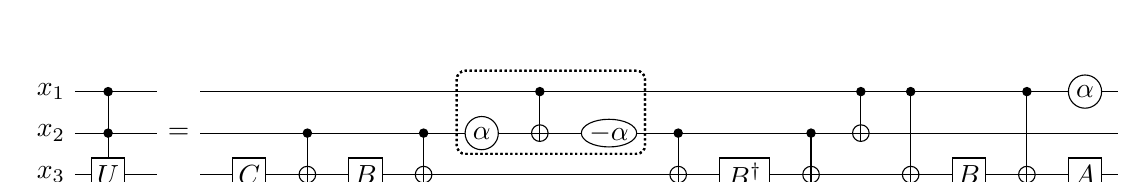
\begin{tikzpicture}[scale=1.000000,x=1pt,y=1pt]
\filldraw[color=white] (0.000000, -7.500000) rectangle (377.000000, 37.500000);
% Drawing wires
% Line 1: a3 W x_3
\draw[color=black] (0.000000,30.000000) -- (377.000000,30.000000);
\draw[color=black] (0.000000,30.000000) node[left] {$x_1$};
% Line 2: a2 W x_2
\draw[color=black] (0.000000,15.000000) -- (377.000000,15.000000);
\draw[color=black] (0.000000,15.000000) node[left] {$x_2$};
% Line 3: a1 W x_1
\draw[color=black] (0.000000,0.000000) -- (377.000000,0.000000);
\draw[color=black] (0.000000,0.000000) node[left] {$x_3$};
% Done with wires; drawing gates
% Line 4: a1 G $U$ a2 a3
\draw (12.000000,30.000000) -- (12.000000,0.000000);
\begin{scope}
\draw[fill=white] (12.000000, -0.000000) +(-45.000000:8.485281pt and 8.485281pt) -- +(45.000000:8.485281pt and 8.485281pt) -- +(135.000000:8.485281pt and 8.485281pt) -- +(225.000000:8.485281pt and 8.485281pt) -- cycle;
\clip (12.000000, -0.000000) +(-45.000000:8.485281pt and 8.485281pt) -- +(45.000000:8.485281pt and 8.485281pt) -- +(135.000000:8.485281pt and 8.485281pt) -- +(225.000000:8.485281pt and 8.485281pt) -- cycle;
\draw (12.000000, -0.000000) node {$U$};
\end{scope}
\filldraw (12.000000, 15.000000) circle(1.500000pt);
\filldraw (12.000000, 30.000000) circle(1.500000pt);
% Line 5: =
\draw[fill=white,color=white] (30.000000, -6.000000) rectangle (45.000000, 36.000000);
\draw (37.500000, 15.000000) node {$=$};
% Line 6: a1 G $C$
\begin{scope}
\draw[fill=white] (63.000000, -0.000000) +(-45.000000:8.485281pt and 8.485281pt) -- +(45.000000:8.485281pt and 8.485281pt) -- +(135.000000:8.485281pt and 8.485281pt) -- +(225.000000:8.485281pt and 8.485281pt) -- cycle;
\clip (63.000000, -0.000000) +(-45.000000:8.485281pt and 8.485281pt) -- +(45.000000:8.485281pt and 8.485281pt) -- +(135.000000:8.485281pt and 8.485281pt) -- +(225.000000:8.485281pt and 8.485281pt) -- cycle;
\draw (63.000000, -0.000000) node {$C$};
\end{scope}
% Line 7: +a1 a2
\draw (84.000000,15.000000) -- (84.000000,0.000000);
\begin{scope}
\draw[fill=white] (84.000000, 0.000000) circle(3.000000pt);
\clip (84.000000, 0.000000) circle(3.000000pt);
\draw (81.000000, 0.000000) -- (87.000000, 0.000000);
\draw (84.000000, -3.000000) -- (84.000000, 3.000000);
\end{scope}
\filldraw (84.000000, 15.000000) circle(1.500000pt);
% Line 8: a1 G $B$
\begin{scope}
\draw[fill=white] (105.000000, -0.000000) +(-45.000000:8.485281pt and 8.485281pt) -- +(45.000000:8.485281pt and 8.485281pt) -- +(135.000000:8.485281pt and 8.485281pt) -- +(225.000000:8.485281pt and 8.485281pt) -- cycle;
\clip (105.000000, -0.000000) +(-45.000000:8.485281pt and 8.485281pt) -- +(45.000000:8.485281pt and 8.485281pt) -- +(135.000000:8.485281pt and 8.485281pt) -- +(225.000000:8.485281pt and 8.485281pt) -- cycle;
\draw (105.000000, -0.000000) node {$B$};
\end{scope}
% Line 9: +a1 a2
\draw (126.000000,15.000000) -- (126.000000,0.000000);
\begin{scope}
\draw[fill=white] (126.000000, 0.000000) circle(3.000000pt);
\clip (126.000000, 0.000000) circle(3.000000pt);
\draw (123.000000, 0.000000) -- (129.000000, 0.000000);
\draw (126.000000, -3.000000) -- (126.000000, 3.000000);
\end{scope}
\filldraw (126.000000, 15.000000) circle(1.500000pt);
% Line 10: TOUCH
% Line 11: a2 P $\alpha$
\begin{scope}
\draw[fill=white] (147.000000, 15.000000) circle(6.000000pt);
\clip (147.000000, 15.000000) circle(6.000000pt);
\draw (147.000000, 15.000000) node {$\alpha$};
\end{scope}
% Line 12: +a2 a3
\draw (168.000000,30.000000) -- (168.000000,15.000000);
\begin{scope}
\draw[fill=white] (168.000000, 15.000000) circle(3.000000pt);
\clip (168.000000, 15.000000) circle(3.000000pt);
\draw (165.000000, 15.000000) -- (171.000000, 15.000000);
\draw (168.000000, 12.000000) -- (168.000000, 18.000000);
\end{scope}
\filldraw (168.000000, 30.000000) circle(1.500000pt);
% Line 13: a2 P $-\alpha$ height=10 width=20
\begin{scope}
\draw[fill=white] (193.000000, 15.000000) ellipse(10.000000pt and 5.000000pt);
\clip (193.000000, 15.000000) ellipse(10.000000pt and 5.000000pt);
\draw (193.000000, 15.000000) node {$-\alpha$};
\end{scope}
% Line 15: +a1 a2
\draw (218.000000,15.000000) -- (218.000000,0.000000);
\begin{scope}
\draw[fill=white] (218.000000, 0.000000) circle(3.000000pt);
\clip (218.000000, 0.000000) circle(3.000000pt);
\draw (215.000000, 0.000000) -- (221.000000, 0.000000);
\draw (218.000000, -3.000000) -- (218.000000, 3.000000);
\end{scope}
\filldraw (218.000000, 15.000000) circle(1.500000pt);
% Line 16: a1 G $B^\dagger$ width=18
\begin{scope}
\draw[fill=white] (242.000000, -0.000000) +(-45.000000:12.727922pt and 8.485281pt) -- +(45.000000:12.727922pt and 8.485281pt) -- +(135.000000:12.727922pt and 8.485281pt) -- +(225.000000:12.727922pt and 8.485281pt) -- cycle;
\clip (242.000000, -0.000000) +(-45.000000:12.727922pt and 8.485281pt) -- +(45.000000:12.727922pt and 8.485281pt) -- +(135.000000:12.727922pt and 8.485281pt) -- +(225.000000:12.727922pt and 8.485281pt) -- cycle;
\draw (242.000000, -0.000000) node {$B^\dagger$};
\end{scope}
% Line 17: +a1 a2
\draw (266.000000,15.000000) -- (266.000000,0.000000);
\begin{scope}
\draw[fill=white] (266.000000, 0.000000) circle(3.000000pt);
\clip (266.000000, 0.000000) circle(3.000000pt);
\draw (263.000000, 0.000000) -- (269.000000, 0.000000);
\draw (266.000000, -3.000000) -- (266.000000, 3.000000);
\end{scope}
\filldraw (266.000000, 15.000000) circle(1.500000pt);
% Line 18: +a2 a3
\draw (284.000000,30.000000) -- (284.000000,15.000000);
\begin{scope}
\draw[fill=white] (284.000000, 15.000000) circle(3.000000pt);
\clip (284.000000, 15.000000) circle(3.000000pt);
\draw (281.000000, 15.000000) -- (287.000000, 15.000000);
\draw (284.000000, 12.000000) -- (284.000000, 18.000000);
\end{scope}
\filldraw (284.000000, 30.000000) circle(1.500000pt);
% Line 19: +a1 a3
\draw (302.000000,30.000000) -- (302.000000,0.000000);
\begin{scope}
\draw[fill=white] (302.000000, 0.000000) circle(3.000000pt);
\clip (302.000000, 0.000000) circle(3.000000pt);
\draw (299.000000, 0.000000) -- (305.000000, 0.000000);
\draw (302.000000, -3.000000) -- (302.000000, 3.000000);
\end{scope}
\filldraw (302.000000, 30.000000) circle(1.500000pt);
% Line 20: a1 G $B$
\begin{scope}
\draw[fill=white] (323.000000, -0.000000) +(-45.000000:8.485281pt and 8.485281pt) -- +(45.000000:8.485281pt and 8.485281pt) -- +(135.000000:8.485281pt and 8.485281pt) -- +(225.000000:8.485281pt and 8.485281pt) -- cycle;
\clip (323.000000, -0.000000) +(-45.000000:8.485281pt and 8.485281pt) -- +(45.000000:8.485281pt and 8.485281pt) -- +(135.000000:8.485281pt and 8.485281pt) -- +(225.000000:8.485281pt and 8.485281pt) -- cycle;
\draw (323.000000, -0.000000) node {$B$};
\end{scope}
% Line 21: +a1 a3
\draw (344.000000,30.000000) -- (344.000000,0.000000);
\begin{scope}
\draw[fill=white] (344.000000, 0.000000) circle(3.000000pt);
\clip (344.000000, 0.000000) circle(3.000000pt);
\draw (341.000000, 0.000000) -- (347.000000, 0.000000);
\draw (344.000000, -3.000000) -- (344.000000, 3.000000);
\end{scope}
\filldraw (344.000000, 30.000000) circle(1.500000pt);
% Line 22: a1 G $A$
\begin{scope}
\draw[fill=white] (365.000000, -0.000000) +(-45.000000:8.485281pt and 8.485281pt) -- +(45.000000:8.485281pt and 8.485281pt) -- +(135.000000:8.485281pt and 8.485281pt) -- +(225.000000:8.485281pt and 8.485281pt) -- cycle;
\clip (365.000000, -0.000000) +(-45.000000:8.485281pt and 8.485281pt) -- +(45.000000:8.485281pt and 8.485281pt) -- +(135.000000:8.485281pt and 8.485281pt) -- +(225.000000:8.485281pt and 8.485281pt) -- cycle;
\draw (365.000000, -0.000000) node {$A$};
\end{scope}
% Line 23: a3 P $\alpha$
\begin{scope}
\draw[fill=white] (365.000000, 30.000000) circle(6.000000pt);
\clip (365.000000, 30.000000) circle(6.000000pt);
\draw (365.000000, 30.000000) node {$\alpha$};
\end{scope}
% Done with gates; drawing ending labels
% Done with ending labels; drawing cut lines and comments
% Line 14: a3 a2 @  3 color=black style=densely_dotted,thick,rounded_corners=3pt
\draw[draw opacity=1.000000,fill opacity=0.200000,color=black,densely dotted,thick,rounded corners=3pt] (138.000000,37.500000) rectangle (206.000000,7.500000);
\draw[draw opacity=1.000000,fill opacity=0.200000,color=black,densely dotted,thick,rounded corners=3pt] (138.000000,37.500000) rectangle (206.000000,7.500000);
% Done with comments
\end{tikzpicture}
\end{center}
\vspace{-10pt}
where we've drawn attention to the grouped $\alpha$, $-\alpha$, and \CNOT\ because we will investigate them as a group.  First the group must gain another \CNOT.  The \CNOT\ we'll gain is the 6th, but to gain it we need to temporarily introduce more \CNOT s.  Neither having been targeted by a \CNOT\ prior, the result of the third \CNOT\ is to calculate the ``parity'' of $\ket{x_1}$ and $\ket{x_2}$ in-place in $\ket{x_2}$ (phase of $\ket{x_2}$ ignored).  The 4th and 5th \CNOT s are then controlled by this parity. We can move the 6-th \CNOT\ to before the 4th, which will uncompute the parity (but not the phase), but we'll need to reconfigure \CNOT's 4 and 5 so that the result is once again a \NOT\ applied to $\ket{x_3}$ controlled by the \underline{parity} of $\ket{x_1}$ and $\ket{x_2}$, not just a \NOT\ controlled by $\ket{x_2}$.  To do this, note that applying \CNOT s to $\ket{x_3}$ controlled by $\ket{x_1}$, then another controlled by $\ket{x_2}$ results in a \NOT\ applied to $\ket{x_3}$ if and only if $\ket{x_1}\ket{x_2} = \ket{0}\ket{1}\mathrm{\ or\ }\ket{1}\ket{0}$, \textit{i.e.} a \CNOT\ controlled by the parity of $\ket{x_1}\ket{x_2}$.  So, we arrive at
\begin{center}
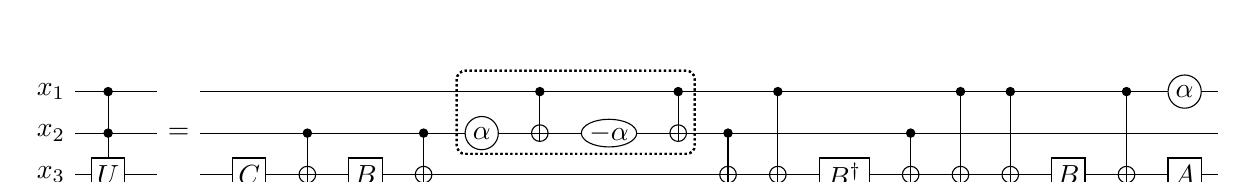
\begin{tikzpicture}[scale=1.000000,x=1pt,y=1pt]
\filldraw[color=white] (0.000000, -7.500000) rectangle (413.000000, 37.500000);
% Drawing wires
% Line 1: a3 W x_3
\draw[color=black] (0.000000,30.000000) -- (413.000000,30.000000);
\draw[color=black] (0.000000,30.000000) node[left] {$x_1$};
% Line 2: a2 W x_2
\draw[color=black] (0.000000,15.000000) -- (413.000000,15.000000);
\draw[color=black] (0.000000,15.000000) node[left] {$x_2$};
% Line 3: a1 W x_1
\draw[color=black] (0.000000,0.000000) -- (413.000000,0.000000);
\draw[color=black] (0.000000,0.000000) node[left] {$x_3$};
% Done with wires; drawing gates
% Line 4: a1 G $U$ a2 a3
\draw (12.000000,30.000000) -- (12.000000,0.000000);
\begin{scope}
\draw[fill=white] (12.000000, -0.000000) +(-45.000000:8.485281pt and 8.485281pt) -- +(45.000000:8.485281pt and 8.485281pt) -- +(135.000000:8.485281pt and 8.485281pt) -- +(225.000000:8.485281pt and 8.485281pt) -- cycle;
\clip (12.000000, -0.000000) +(-45.000000:8.485281pt and 8.485281pt) -- +(45.000000:8.485281pt and 8.485281pt) -- +(135.000000:8.485281pt and 8.485281pt) -- +(225.000000:8.485281pt and 8.485281pt) -- cycle;
\draw (12.000000, -0.000000) node {$U$};
\end{scope}
\filldraw (12.000000, 15.000000) circle(1.500000pt);
\filldraw (12.000000, 30.000000) circle(1.500000pt);
% Line 5: =
\draw[fill=white,color=white] (30.000000, -6.000000) rectangle (45.000000, 36.000000);
\draw (37.500000, 15.000000) node {$=$};
% Line 6: a1 G $C$
\begin{scope}
\draw[fill=white] (63.000000, -0.000000) +(-45.000000:8.485281pt and 8.485281pt) -- +(45.000000:8.485281pt and 8.485281pt) -- +(135.000000:8.485281pt and 8.485281pt) -- +(225.000000:8.485281pt and 8.485281pt) -- cycle;
\clip (63.000000, -0.000000) +(-45.000000:8.485281pt and 8.485281pt) -- +(45.000000:8.485281pt and 8.485281pt) -- +(135.000000:8.485281pt and 8.485281pt) -- +(225.000000:8.485281pt and 8.485281pt) -- cycle;
\draw (63.000000, -0.000000) node {$C$};
\end{scope}
% Line 7: +a1 a2
\draw (84.000000,15.000000) -- (84.000000,0.000000);
\begin{scope}
\draw[fill=white] (84.000000, 0.000000) circle(3.000000pt);
\clip (84.000000, 0.000000) circle(3.000000pt);
\draw (81.000000, 0.000000) -- (87.000000, 0.000000);
\draw (84.000000, -3.000000) -- (84.000000, 3.000000);
\end{scope}
\filldraw (84.000000, 15.000000) circle(1.500000pt);
% Line 8: a1 G $B$
\begin{scope}
\draw[fill=white] (105.000000, -0.000000) +(-45.000000:8.485281pt and 8.485281pt) -- +(45.000000:8.485281pt and 8.485281pt) -- +(135.000000:8.485281pt and 8.485281pt) -- +(225.000000:8.485281pt and 8.485281pt) -- cycle;
\clip (105.000000, -0.000000) +(-45.000000:8.485281pt and 8.485281pt) -- +(45.000000:8.485281pt and 8.485281pt) -- +(135.000000:8.485281pt and 8.485281pt) -- +(225.000000:8.485281pt and 8.485281pt) -- cycle;
\draw (105.000000, -0.000000) node {$B$};
\end{scope}
% Line 9: +a1 a2
\draw (126.000000,15.000000) -- (126.000000,0.000000);
\begin{scope}
\draw[fill=white] (126.000000, 0.000000) circle(3.000000pt);
\clip (126.000000, 0.000000) circle(3.000000pt);
\draw (123.000000, 0.000000) -- (129.000000, 0.000000);
\draw (126.000000, -3.000000) -- (126.000000, 3.000000);
\end{scope}
\filldraw (126.000000, 15.000000) circle(1.500000pt);
% Line 10: TOUCH
% Line 11: a2 P $\alpha$
\begin{scope}
\draw[fill=white] (147.000000, 15.000000) circle(6.000000pt);
\clip (147.000000, 15.000000) circle(6.000000pt);
\draw (147.000000, 15.000000) node {$\alpha$};
\end{scope}
% Line 12: +a2 a3
\draw (168.000000,30.000000) -- (168.000000,15.000000);
\begin{scope}
\draw[fill=white] (168.000000, 15.000000) circle(3.000000pt);
\clip (168.000000, 15.000000) circle(3.000000pt);
\draw (165.000000, 15.000000) -- (171.000000, 15.000000);
\draw (168.000000, 12.000000) -- (168.000000, 18.000000);
\end{scope}
\filldraw (168.000000, 30.000000) circle(1.500000pt);
% Line 13: a2 P $-\alpha$ height=10 width=20
\begin{scope}
\draw[fill=white] (193.000000, 15.000000) ellipse(10.000000pt and 5.000000pt);
\clip (193.000000, 15.000000) ellipse(10.000000pt and 5.000000pt);
\draw (193.000000, 15.000000) node {$-\alpha$};
\end{scope}
% Line 14: +a2 a3
\draw (218.000000,30.000000) -- (218.000000,15.000000);
\begin{scope}
\draw[fill=white] (218.000000, 15.000000) circle(3.000000pt);
\clip (218.000000, 15.000000) circle(3.000000pt);
\draw (215.000000, 15.000000) -- (221.000000, 15.000000);
\draw (218.000000, 12.000000) -- (218.000000, 18.000000);
\end{scope}
\filldraw (218.000000, 30.000000) circle(1.500000pt);
% Line 16: +a1 a2
\draw (236.000000,15.000000) -- (236.000000,0.000000);
\begin{scope}
\draw[fill=white] (236.000000, 0.000000) circle(3.000000pt);
\clip (236.000000, 0.000000) circle(3.000000pt);
\draw (233.000000, 0.000000) -- (239.000000, 0.000000);
\draw (236.000000, -3.000000) -- (236.000000, 3.000000);
\end{scope}
\filldraw (236.000000, 15.000000) circle(1.500000pt);
% Line 17: +a1 a3
\draw (254.000000,30.000000) -- (254.000000,0.000000);
\begin{scope}
\draw[fill=white] (254.000000, 0.000000) circle(3.000000pt);
\clip (254.000000, 0.000000) circle(3.000000pt);
\draw (251.000000, 0.000000) -- (257.000000, 0.000000);
\draw (254.000000, -3.000000) -- (254.000000, 3.000000);
\end{scope}
\filldraw (254.000000, 30.000000) circle(1.500000pt);
% Line 18: a1 G $B^\dagger$ width=18
\begin{scope}
\draw[fill=white] (278.000000, -0.000000) +(-45.000000:12.727922pt and 8.485281pt) -- +(45.000000:12.727922pt and 8.485281pt) -- +(135.000000:12.727922pt and 8.485281pt) -- +(225.000000:12.727922pt and 8.485281pt) -- cycle;
\clip (278.000000, -0.000000) +(-45.000000:12.727922pt and 8.485281pt) -- +(45.000000:12.727922pt and 8.485281pt) -- +(135.000000:12.727922pt and 8.485281pt) -- +(225.000000:12.727922pt and 8.485281pt) -- cycle;
\draw (278.000000, -0.000000) node {$B^\dagger$};
\end{scope}
% Line 19: +a1 a2
\draw (302.000000,15.000000) -- (302.000000,0.000000);
\begin{scope}
\draw[fill=white] (302.000000, 0.000000) circle(3.000000pt);
\clip (302.000000, 0.000000) circle(3.000000pt);
\draw (299.000000, 0.000000) -- (305.000000, 0.000000);
\draw (302.000000, -3.000000) -- (302.000000, 3.000000);
\end{scope}
\filldraw (302.000000, 15.000000) circle(1.500000pt);
% Line 20: +a1 a3
\draw (320.000000,30.000000) -- (320.000000,0.000000);
\begin{scope}
\draw[fill=white] (320.000000, 0.000000) circle(3.000000pt);
\clip (320.000000, 0.000000) circle(3.000000pt);
\draw (317.000000, 0.000000) -- (323.000000, 0.000000);
\draw (320.000000, -3.000000) -- (320.000000, 3.000000);
\end{scope}
\filldraw (320.000000, 30.000000) circle(1.500000pt);
% Line 21: +a1 a3
\draw (338.000000,30.000000) -- (338.000000,0.000000);
\begin{scope}
\draw[fill=white] (338.000000, 0.000000) circle(3.000000pt);
\clip (338.000000, 0.000000) circle(3.000000pt);
\draw (335.000000, 0.000000) -- (341.000000, 0.000000);
\draw (338.000000, -3.000000) -- (338.000000, 3.000000);
\end{scope}
\filldraw (338.000000, 30.000000) circle(1.500000pt);
% Line 22: a1 G $B$
\begin{scope}
\draw[fill=white] (359.000000, -0.000000) +(-45.000000:8.485281pt and 8.485281pt) -- +(45.000000:8.485281pt and 8.485281pt) -- +(135.000000:8.485281pt and 8.485281pt) -- +(225.000000:8.485281pt and 8.485281pt) -- cycle;
\clip (359.000000, -0.000000) +(-45.000000:8.485281pt and 8.485281pt) -- +(45.000000:8.485281pt and 8.485281pt) -- +(135.000000:8.485281pt and 8.485281pt) -- +(225.000000:8.485281pt and 8.485281pt) -- cycle;
\draw (359.000000, -0.000000) node {$B$};
\end{scope}
% Line 23: +a1 a3
\draw (380.000000,30.000000) -- (380.000000,0.000000);
\begin{scope}
\draw[fill=white] (380.000000, 0.000000) circle(3.000000pt);
\clip (380.000000, 0.000000) circle(3.000000pt);
\draw (377.000000, 0.000000) -- (383.000000, 0.000000);
\draw (380.000000, -3.000000) -- (380.000000, 3.000000);
\end{scope}
\filldraw (380.000000, 30.000000) circle(1.500000pt);
% Line 24: a1 G $A$
\begin{scope}
\draw[fill=white] (401.000000, -0.000000) +(-45.000000:8.485281pt and 8.485281pt) -- +(45.000000:8.485281pt and 8.485281pt) -- +(135.000000:8.485281pt and 8.485281pt) -- +(225.000000:8.485281pt and 8.485281pt) -- cycle;
\clip (401.000000, -0.000000) +(-45.000000:8.485281pt and 8.485281pt) -- +(45.000000:8.485281pt and 8.485281pt) -- +(135.000000:8.485281pt and 8.485281pt) -- +(225.000000:8.485281pt and 8.485281pt) -- cycle;
\draw (401.000000, -0.000000) node {$A$};
\end{scope}
% Line 25: a3 P $\alpha$
\begin{scope}
\draw[fill=white] (401.000000, 30.000000) circle(6.000000pt);
\clip (401.000000, 30.000000) circle(6.000000pt);
\draw (401.000000, 30.000000) node {$\alpha$};
\end{scope}
% Done with gates; drawing ending labels
% Done with ending labels; drawing cut lines and comments
% Line 15: a3 a2 @  4 color=black style=densely_dotted,thick,rounded_corners=3pt
\draw[draw opacity=1.000000,fill opacity=0.200000,color=black,densely dotted,thick,rounded corners=3pt] (138.000000,37.500000) rectangle (224.000000,7.500000);
\draw[draw opacity=1.000000,fill opacity=0.200000,color=black,densely dotted,thick,rounded corners=3pt] (138.000000,37.500000) rectangle (224.000000,7.500000);
% Done with comments
\end{tikzpicture}
\end{center}
\vspace{-10pt}
Now, the operation of the grouped gates on $\ket{x_1}\ket{x_2}$ can be expressed as
$$
\begin{bmatrix} 1 & 0 & 0 & 0 \\ 0 & 1 & 0 & 0 \\ 0 & 0 & 0 & 1 \\ 0 & 0 & 1 & 0 \end{bmatrix}
\begin{bmatrix} 1 & 0 & 0 & 0 \\ 0 & e^{-i\alpha} & 0 & 0 \\ 0 & 0 & 1 & 0 \\ 0 & 0& 0& e^{-i\alpha}\end{bmatrix}
\begin{bmatrix} 1 & 0 & 0 & 0 \\ 0 & 1 & 0 & 0 \\ 0 & 0 & 0 & 1 \\ 0 & 0 & 1 & 0 \end{bmatrix}
\begin{bmatrix} 1 & 0 & 0 & 0 \\ 0 & e^{i\alpha} & 0 & 0 \\ 0 & 0 & 1 & 0 \\ 0 & 0& 0& e^{i\alpha}\end{bmatrix}
=
\begin{bmatrix} 1 & 0 & 0 & 0 \\ 0 & 1 & 0 & 0 \\ 0 & 0 & e^{-i\alpha} & 0 \\ 0 & 0& 0& e^{i\alpha}\end{bmatrix}
$$
Being diagonal, the group can be transposed with any gate not targeting $\ket{x_1}$ or $\ket{x_2}$.  Doing so will only change when the relative phase corrections are performed in the circuit, not the final result.  We'll move it to the end to group the action only on $\ket{x_1}$ and $\ket{x_2}$. While we're at it, we'll move the final $\alpha$ to the start of the group, since it is diagonal and can be transposed with any gate not targeting $\ket{x_1}$.  Doing this allows the two \CNOT$(x_2,x_3)$s previously beside the group to cancel, along with the consecutive \CNOT$(x_1,x_3)$s between the $B^\dagger$ and $B$, giving the final circuit below with 8 single-qubit gates (including the $\alpha$'s and $-\alpha$) and 6 \CNOT s.
\begin{center}
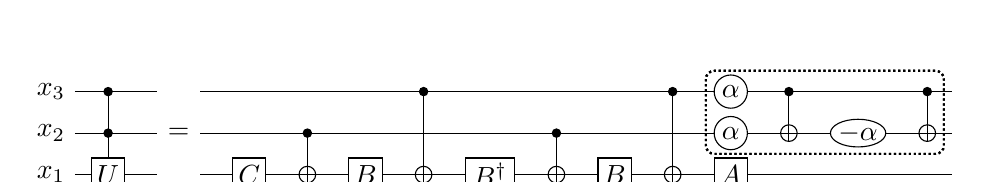
\begin{tikzpicture}[scale=1.000000,x=1pt,y=1pt]
\filldraw[color=white] (0.000000, -7.500000) rectangle (317.000000, 37.500000);
% Drawing wires
% Line 1: a3 W x_3
\draw[color=black] (0.000000,30.000000) -- (317.000000,30.000000);
\draw[color=black] (0.000000,30.000000) node[left] {$x_3$};
% Line 2: a2 W x_2
\draw[color=black] (0.000000,15.000000) -- (317.000000,15.000000);
\draw[color=black] (0.000000,15.000000) node[left] {$x_2$};
% Line 3: a1 W x_1
\draw[color=black] (0.000000,0.000000) -- (317.000000,0.000000);
\draw[color=black] (0.000000,0.000000) node[left] {$x_1$};
% Done with wires; drawing gates
% Line 4: a1 G $U$ a2 a3
\draw (12.000000,30.000000) -- (12.000000,0.000000);
\begin{scope}
\draw[fill=white] (12.000000, -0.000000) +(-45.000000:8.485281pt and 8.485281pt) -- +(45.000000:8.485281pt and 8.485281pt) -- +(135.000000:8.485281pt and 8.485281pt) -- +(225.000000:8.485281pt and 8.485281pt) -- cycle;
\clip (12.000000, -0.000000) +(-45.000000:8.485281pt and 8.485281pt) -- +(45.000000:8.485281pt and 8.485281pt) -- +(135.000000:8.485281pt and 8.485281pt) -- +(225.000000:8.485281pt and 8.485281pt) -- cycle;
\draw (12.000000, -0.000000) node {$U$};
\end{scope}
\filldraw (12.000000, 15.000000) circle(1.500000pt);
\filldraw (12.000000, 30.000000) circle(1.500000pt);
% Line 5: =
\draw[fill=white,color=white] (30.000000, -6.000000) rectangle (45.000000, 36.000000);
\draw (37.500000, 15.000000) node {$=$};
% Line 6: a1 G $C$
\begin{scope}
\draw[fill=white] (63.000000, -0.000000) +(-45.000000:8.485281pt and 8.485281pt) -- +(45.000000:8.485281pt and 8.485281pt) -- +(135.000000:8.485281pt and 8.485281pt) -- +(225.000000:8.485281pt and 8.485281pt) -- cycle;
\clip (63.000000, -0.000000) +(-45.000000:8.485281pt and 8.485281pt) -- +(45.000000:8.485281pt and 8.485281pt) -- +(135.000000:8.485281pt and 8.485281pt) -- +(225.000000:8.485281pt and 8.485281pt) -- cycle;
\draw (63.000000, -0.000000) node {$C$};
\end{scope}
% Line 7: +a1 a2
\draw (84.000000,15.000000) -- (84.000000,0.000000);
\begin{scope}
\draw[fill=white] (84.000000, 0.000000) circle(3.000000pt);
\clip (84.000000, 0.000000) circle(3.000000pt);
\draw (81.000000, 0.000000) -- (87.000000, 0.000000);
\draw (84.000000, -3.000000) -- (84.000000, 3.000000);
\end{scope}
\filldraw (84.000000, 15.000000) circle(1.500000pt);
% Line 8: a1 G $B$
\begin{scope}
\draw[fill=white] (105.000000, -0.000000) +(-45.000000:8.485281pt and 8.485281pt) -- +(45.000000:8.485281pt and 8.485281pt) -- +(135.000000:8.485281pt and 8.485281pt) -- +(225.000000:8.485281pt and 8.485281pt) -- cycle;
\clip (105.000000, -0.000000) +(-45.000000:8.485281pt and 8.485281pt) -- +(45.000000:8.485281pt and 8.485281pt) -- +(135.000000:8.485281pt and 8.485281pt) -- +(225.000000:8.485281pt and 8.485281pt) -- cycle;
\draw (105.000000, -0.000000) node {$B$};
\end{scope}
% Line 9: +a1 a3
\draw (126.000000,30.000000) -- (126.000000,0.000000);
\begin{scope}
\draw[fill=white] (126.000000, 0.000000) circle(3.000000pt);
\clip (126.000000, 0.000000) circle(3.000000pt);
\draw (123.000000, 0.000000) -- (129.000000, 0.000000);
\draw (126.000000, -3.000000) -- (126.000000, 3.000000);
\end{scope}
\filldraw (126.000000, 30.000000) circle(1.500000pt);
% Line 10: a1 G $B^\dagger$ width=18
\begin{scope}
\draw[fill=white] (150.000000, -0.000000) +(-45.000000:12.727922pt and 8.485281pt) -- +(45.000000:12.727922pt and 8.485281pt) -- +(135.000000:12.727922pt and 8.485281pt) -- +(225.000000:12.727922pt and 8.485281pt) -- cycle;
\clip (150.000000, -0.000000) +(-45.000000:12.727922pt and 8.485281pt) -- +(45.000000:12.727922pt and 8.485281pt) -- +(135.000000:12.727922pt and 8.485281pt) -- +(225.000000:12.727922pt and 8.485281pt) -- cycle;
\draw (150.000000, -0.000000) node {$B^\dagger$};
\end{scope}
% Line 11: +a1 a2
\draw (174.000000,15.000000) -- (174.000000,0.000000);
\begin{scope}
\draw[fill=white] (174.000000, 0.000000) circle(3.000000pt);
\clip (174.000000, 0.000000) circle(3.000000pt);
\draw (171.000000, 0.000000) -- (177.000000, 0.000000);
\draw (174.000000, -3.000000) -- (174.000000, 3.000000);
\end{scope}
\filldraw (174.000000, 15.000000) circle(1.500000pt);
% Line 12: a1 G $B$
\begin{scope}
\draw[fill=white] (195.000000, -0.000000) +(-45.000000:8.485281pt and 8.485281pt) -- +(45.000000:8.485281pt and 8.485281pt) -- +(135.000000:8.485281pt and 8.485281pt) -- +(225.000000:8.485281pt and 8.485281pt) -- cycle;
\clip (195.000000, -0.000000) +(-45.000000:8.485281pt and 8.485281pt) -- +(45.000000:8.485281pt and 8.485281pt) -- +(135.000000:8.485281pt and 8.485281pt) -- +(225.000000:8.485281pt and 8.485281pt) -- cycle;
\draw (195.000000, -0.000000) node {$B$};
\end{scope}
% Line 13: +a1 a3
\draw (216.000000,30.000000) -- (216.000000,0.000000);
\begin{scope}
\draw[fill=white] (216.000000, 0.000000) circle(3.000000pt);
\clip (216.000000, 0.000000) circle(3.000000pt);
\draw (213.000000, 0.000000) -- (219.000000, 0.000000);
\draw (216.000000, -3.000000) -- (216.000000, 3.000000);
\end{scope}
\filldraw (216.000000, 30.000000) circle(1.500000pt);
% Line 14: TOUCH
% Line 15: a1 G $A$
\begin{scope}
\draw[fill=white] (237.000000, -0.000000) +(-45.000000:8.485281pt and 8.485281pt) -- +(45.000000:8.485281pt and 8.485281pt) -- +(135.000000:8.485281pt and 8.485281pt) -- +(225.000000:8.485281pt and 8.485281pt) -- cycle;
\clip (237.000000, -0.000000) +(-45.000000:8.485281pt and 8.485281pt) -- +(45.000000:8.485281pt and 8.485281pt) -- +(135.000000:8.485281pt and 8.485281pt) -- +(225.000000:8.485281pt and 8.485281pt) -- cycle;
\draw (237.000000, -0.000000) node {$A$};
\end{scope}
% Line 16: a3 P $\alpha$
\begin{scope}
\draw[fill=white] (237.000000, 30.000000) circle(6.000000pt);
\clip (237.000000, 30.000000) circle(6.000000pt);
\draw (237.000000, 30.000000) node {$\alpha$};
\end{scope}
% Line 17: a2 P $\alpha$
\begin{scope}
\draw[fill=white] (237.000000, 15.000000) circle(6.000000pt);
\clip (237.000000, 15.000000) circle(6.000000pt);
\draw (237.000000, 15.000000) node {$\alpha$};
\end{scope}
% Line 18: +a2 a3
\draw (258.000000,30.000000) -- (258.000000,15.000000);
\begin{scope}
\draw[fill=white] (258.000000, 15.000000) circle(3.000000pt);
\clip (258.000000, 15.000000) circle(3.000000pt);
\draw (255.000000, 15.000000) -- (261.000000, 15.000000);
\draw (258.000000, 12.000000) -- (258.000000, 18.000000);
\end{scope}
\filldraw (258.000000, 30.000000) circle(1.500000pt);
% Line 19: a2 P $-\alpha$ height=10 width=20
\begin{scope}
\draw[fill=white] (283.000000, 15.000000) ellipse(10.000000pt and 5.000000pt);
\clip (283.000000, 15.000000) ellipse(10.000000pt and 5.000000pt);
\draw (283.000000, 15.000000) node {$-\alpha$};
\end{scope}
% Line 20: +a2 a3
\draw (308.000000,30.000000) -- (308.000000,15.000000);
\begin{scope}
\draw[fill=white] (308.000000, 15.000000) circle(3.000000pt);
\clip (308.000000, 15.000000) circle(3.000000pt);
\draw (305.000000, 15.000000) -- (311.000000, 15.000000);
\draw (308.000000, 12.000000) -- (308.000000, 18.000000);
\end{scope}
\filldraw (308.000000, 30.000000) circle(1.500000pt);
% Done with gates; drawing ending labels
% Done with ending labels; drawing cut lines and comments
% Line 21: a3 a2 @  4 color=black style=densely_dotted,thick,rounded_corners=3pt
\draw[draw opacity=1.000000,fill opacity=0.200000,color=black,densely dotted,thick,rounded corners=3pt] (228.000000,37.500000) rectangle (314.000000,7.500000);
\draw[draw opacity=1.000000,fill opacity=0.200000,color=black,densely dotted,thick,rounded corners=3pt] (228.000000,37.500000) rectangle (314.000000,7.500000);
% Done with comments
\end{tikzpicture}
\end{center}
\Textbf{4.23}
\Textbf{4.24} Verify that Figure 4.9 implements the Toffoli gate.
\begin{center}
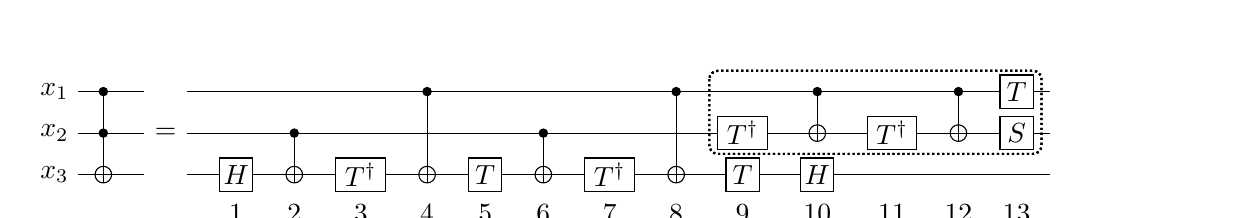
\begin{tikzpicture}[scale=1.000000,x=1pt,y=1pt]
\filldraw[color=white] (0.000000, -7.500000) rectangle (351.000000, 37.500000);
% Drawing wires
% Line 1: a3 W x_1
\draw[color=black] (0.000000,30.000000) -- (351.000000,30.000000);
\draw[color=black] (0.000000,30.000000) node[left] {$x_1$};
% Line 2: a2 W x_2
\draw[color=black] (0.000000,15.000000) -- (351.000000,15.000000);
\draw[color=black] (0.000000,15.000000) node[left] {$x_2$};
% Line 3: a1 W x_3
\draw[color=black] (0.000000,0.000000) -- (351.000000,0.000000);
\draw[color=black] (0.000000,0.000000) node[left] {$x_3$};
% Done with wires; drawing gates
% Line 4: +a1 a2 a3
\draw (9.000000,30.000000) -- (9.000000,0.000000);
\begin{scope}
\draw[fill=white] (9.000000, 0.000000) circle(3.000000pt);
\clip (9.000000, 0.000000) circle(3.000000pt);
\draw (6.000000, 0.000000) -- (12.000000, 0.000000);
\draw (9.000000, -3.000000) -- (9.000000, 3.000000);
\end{scope}
\filldraw (9.000000, 15.000000) circle(1.500000pt);
\filldraw (9.000000, 30.000000) circle(1.500000pt);
% Line 5: =
\draw[fill=white,color=white] (24.000000, -6.000000) rectangle (39.000000, 36.000000);
\draw (31.500000, 15.000000) node {$=$};
% Line 6: a1 H %% 1
\draw (57.000000, -7.500000) node[text width=144pt,below,text centered] {1};
\begin{scope}
\draw[fill=white] (57.000000, -0.000000) +(-45.000000:8.485281pt and 8.485281pt) -- +(45.000000:8.485281pt and 8.485281pt) -- +(135.000000:8.485281pt and 8.485281pt) -- +(225.000000:8.485281pt and 8.485281pt) -- cycle;
\clip (57.000000, -0.000000) +(-45.000000:8.485281pt and 8.485281pt) -- +(45.000000:8.485281pt and 8.485281pt) -- +(135.000000:8.485281pt and 8.485281pt) -- +(225.000000:8.485281pt and 8.485281pt) -- cycle;
\draw (57.000000, -0.000000) node {$H$};
\end{scope}
% Line 7: +a1 a2 %% 2
\draw (78.000000, -7.500000) node[text width=144pt,below,text centered] {2};
\draw (78.000000,15.000000) -- (78.000000,0.000000);
\begin{scope}
\draw[fill=white] (78.000000, 0.000000) circle(3.000000pt);
\clip (78.000000, 0.000000) circle(3.000000pt);
\draw (75.000000, 0.000000) -- (81.000000, 0.000000);
\draw (78.000000, -3.000000) -- (78.000000, 3.000000);
\end{scope}
\filldraw (78.000000, 15.000000) circle(1.500000pt);
% Line 8: a1 G $T^\dagger$ width=18 %% 3
\draw (102.000000, -7.500000) node[text width=144pt,below,text centered] {3};
\begin{scope}
\draw[fill=white] (102.000000, -0.000000) +(-45.000000:12.727922pt and 8.485281pt) -- +(45.000000:12.727922pt and 8.485281pt) -- +(135.000000:12.727922pt and 8.485281pt) -- +(225.000000:12.727922pt and 8.485281pt) -- cycle;
\clip (102.000000, -0.000000) +(-45.000000:12.727922pt and 8.485281pt) -- +(45.000000:12.727922pt and 8.485281pt) -- +(135.000000:12.727922pt and 8.485281pt) -- +(225.000000:12.727922pt and 8.485281pt) -- cycle;
\draw (102.000000, -0.000000) node {$T^\dagger$};
\end{scope}
% Line 9: +a1 a3 %% 4
\draw (126.000000, -7.500000) node[text width=144pt,below,text centered] {4};
\draw (126.000000,30.000000) -- (126.000000,0.000000);
\begin{scope}
\draw[fill=white] (126.000000, 0.000000) circle(3.000000pt);
\clip (126.000000, 0.000000) circle(3.000000pt);
\draw (123.000000, 0.000000) -- (129.000000, 0.000000);
\draw (126.000000, -3.000000) -- (126.000000, 3.000000);
\end{scope}
\filldraw (126.000000, 30.000000) circle(1.500000pt);
% Line 10: a1 G $T$ %% 5
\draw (147.000000, -7.500000) node[text width=144pt,below,text centered] {5};
\begin{scope}
\draw[fill=white] (147.000000, -0.000000) +(-45.000000:8.485281pt and 8.485281pt) -- +(45.000000:8.485281pt and 8.485281pt) -- +(135.000000:8.485281pt and 8.485281pt) -- +(225.000000:8.485281pt and 8.485281pt) -- cycle;
\clip (147.000000, -0.000000) +(-45.000000:8.485281pt and 8.485281pt) -- +(45.000000:8.485281pt and 8.485281pt) -- +(135.000000:8.485281pt and 8.485281pt) -- +(225.000000:8.485281pt and 8.485281pt) -- cycle;
\draw (147.000000, -0.000000) node {$T$};
\end{scope}
% Line 11: +a1 a2 %% 6
\draw (168.000000, -7.500000) node[text width=144pt,below,text centered] {6};
\draw (168.000000,15.000000) -- (168.000000,0.000000);
\begin{scope}
\draw[fill=white] (168.000000, 0.000000) circle(3.000000pt);
\clip (168.000000, 0.000000) circle(3.000000pt);
\draw (165.000000, 0.000000) -- (171.000000, 0.000000);
\draw (168.000000, -3.000000) -- (168.000000, 3.000000);
\end{scope}
\filldraw (168.000000, 15.000000) circle(1.500000pt);
% Line 12: a1 G $T^\dagger$ width=18 %% 7
\draw (192.000000, -7.500000) node[text width=144pt,below,text centered] {7};
\begin{scope}
\draw[fill=white] (192.000000, -0.000000) +(-45.000000:12.727922pt and 8.485281pt) -- +(45.000000:12.727922pt and 8.485281pt) -- +(135.000000:12.727922pt and 8.485281pt) -- +(225.000000:12.727922pt and 8.485281pt) -- cycle;
\clip (192.000000, -0.000000) +(-45.000000:12.727922pt and 8.485281pt) -- +(45.000000:12.727922pt and 8.485281pt) -- +(135.000000:12.727922pt and 8.485281pt) -- +(225.000000:12.727922pt and 8.485281pt) -- cycle;
\draw (192.000000, -0.000000) node {$T^\dagger$};
\end{scope}
% Line 13: +a1 a3 %% 8
\draw (216.000000, -7.500000) node[text width=144pt,below,text centered] {8};
\draw (216.000000,30.000000) -- (216.000000,0.000000);
\begin{scope}
\draw[fill=white] (216.000000, 0.000000) circle(3.000000pt);
\clip (216.000000, 0.000000) circle(3.000000pt);
\draw (213.000000, 0.000000) -- (219.000000, 0.000000);
\draw (216.000000, -3.000000) -- (216.000000, 3.000000);
\end{scope}
\filldraw (216.000000, 30.000000) circle(1.500000pt);
% Line 14: TOUCH
% Line 15: a2 G $T^\dagger$ width=18
\begin{scope}
\draw[fill=white] (240.000000, 15.000000) +(-45.000000:12.727922pt and 8.485281pt) -- +(45.000000:12.727922pt and 8.485281pt) -- +(135.000000:12.727922pt and 8.485281pt) -- +(225.000000:12.727922pt and 8.485281pt) -- cycle;
\clip (240.000000, 15.000000) +(-45.000000:12.727922pt and 8.485281pt) -- +(45.000000:12.727922pt and 8.485281pt) -- +(135.000000:12.727922pt and 8.485281pt) -- +(225.000000:12.727922pt and 8.485281pt) -- cycle;
\draw (240.000000, 15.000000) node {$T^\dagger$};
\end{scope}
% Line 16: a1 G $T$ %% 9
\draw (240.000000, -7.500000) node[text width=144pt,below,text centered] {9};
\begin{scope}
\draw[fill=white] (240.000000, -0.000000) +(-45.000000:8.485281pt and 8.485281pt) -- +(45.000000:8.485281pt and 8.485281pt) -- +(135.000000:8.485281pt and 8.485281pt) -- +(225.000000:8.485281pt and 8.485281pt) -- cycle;
\clip (240.000000, -0.000000) +(-45.000000:8.485281pt and 8.485281pt) -- +(45.000000:8.485281pt and 8.485281pt) -- +(135.000000:8.485281pt and 8.485281pt) -- +(225.000000:8.485281pt and 8.485281pt) -- cycle;
\draw (240.000000, -0.000000) node {$T$};
\end{scope}
% Line 17: a1 H
\begin{scope}
\draw[fill=white] (267.000000, -0.000000) +(-45.000000:8.485281pt and 8.485281pt) -- +(45.000000:8.485281pt and 8.485281pt) -- +(135.000000:8.485281pt and 8.485281pt) -- +(225.000000:8.485281pt and 8.485281pt) -- cycle;
\clip (267.000000, -0.000000) +(-45.000000:8.485281pt and 8.485281pt) -- +(45.000000:8.485281pt and 8.485281pt) -- +(135.000000:8.485281pt and 8.485281pt) -- +(225.000000:8.485281pt and 8.485281pt) -- cycle;
\draw (267.000000, -0.000000) node {$H$};
\end{scope}
% Line 18: +a2 a3 %% 10
\draw (267.000000, -7.500000) node[text width=144pt,below,text centered] {10};
\draw (267.000000,30.000000) -- (267.000000,15.000000);
\begin{scope}
\draw[fill=white] (267.000000, 15.000000) circle(3.000000pt);
\clip (267.000000, 15.000000) circle(3.000000pt);
\draw (264.000000, 15.000000) -- (270.000000, 15.000000);
\draw (267.000000, 12.000000) -- (267.000000, 18.000000);
\end{scope}
\filldraw (267.000000, 30.000000) circle(1.500000pt);
% Line 19: a2 G $T^\dagger$ width=18 %% 11
\draw (294.000000, -7.500000) node[text width=144pt,below,text centered] {11};
\begin{scope}
\draw[fill=white] (294.000000, 15.000000) +(-45.000000:12.727922pt and 8.485281pt) -- +(45.000000:12.727922pt and 8.485281pt) -- +(135.000000:12.727922pt and 8.485281pt) -- +(225.000000:12.727922pt and 8.485281pt) -- cycle;
\clip (294.000000, 15.000000) +(-45.000000:12.727922pt and 8.485281pt) -- +(45.000000:12.727922pt and 8.485281pt) -- +(135.000000:12.727922pt and 8.485281pt) -- +(225.000000:12.727922pt and 8.485281pt) -- cycle;
\draw (294.000000, 15.000000) node {$T^\dagger$};
\end{scope}
% Line 20: +a2 a3 %% 12
\draw (318.000000, -7.500000) node[text width=144pt,below,text centered] {12};
\draw (318.000000,30.000000) -- (318.000000,15.000000);
\begin{scope}
\draw[fill=white] (318.000000, 15.000000) circle(3.000000pt);
\clip (318.000000, 15.000000) circle(3.000000pt);
\draw (315.000000, 15.000000) -- (321.000000, 15.000000);
\draw (318.000000, 12.000000) -- (318.000000, 18.000000);
\end{scope}
\filldraw (318.000000, 30.000000) circle(1.500000pt);
% Line 21: a3 G $T$
\begin{scope}
\draw[fill=white] (339.000000, 30.000000) +(-45.000000:8.485281pt and 8.485281pt) -- +(45.000000:8.485281pt and 8.485281pt) -- +(135.000000:8.485281pt and 8.485281pt) -- +(225.000000:8.485281pt and 8.485281pt) -- cycle;
\clip (339.000000, 30.000000) +(-45.000000:8.485281pt and 8.485281pt) -- +(45.000000:8.485281pt and 8.485281pt) -- +(135.000000:8.485281pt and 8.485281pt) -- +(225.000000:8.485281pt and 8.485281pt) -- cycle;
\draw (339.000000, 30.000000) node {$T$};
\end{scope}
% Line 22: a2 G $S$ %% 13
\draw (339.000000, -7.500000) node[text width=144pt,below,text centered] {13};
\begin{scope}
\draw[fill=white] (339.000000, 15.000000) +(-45.000000:8.485281pt and 8.485281pt) -- +(45.000000:8.485281pt and 8.485281pt) -- +(135.000000:8.485281pt and 8.485281pt) -- +(225.000000:8.485281pt and 8.485281pt) -- cycle;
\clip (339.000000, 15.000000) +(-45.000000:8.485281pt and 8.485281pt) -- +(45.000000:8.485281pt and 8.485281pt) -- +(135.000000:8.485281pt and 8.485281pt) -- +(225.000000:8.485281pt and 8.485281pt) -- cycle;
\draw (339.000000, 15.000000) node {$S$};
\end{scope}
% Done with gates; drawing ending labels
% Done with ending labels; drawing cut lines and comments
% Line 23: a3 a2 @  5 color=black style=densely_dotted,thick,rounded_corners=3pt
\draw[draw opacity=1.000000,fill opacity=0.200000,color=black,densely dotted,thick,rounded corners=3pt] (228.000000,37.500000) rectangle (348.000000,7.500000);
\draw[draw opacity=1.000000,fill opacity=0.200000,color=black,densely dotted,thick,rounded corners=3pt] (228.000000,37.500000) rectangle (348.000000,7.500000);
% Done with comments
\end{tikzpicture}
\end{center}
\vspace{-15pt}
\Soln Define $V = \frac{1+i}{2}(I-iX), A=HT, B=T^\dagger, C=H$, and $\alpha=\pi/4$.  Note that this choice of $V$ is similar to that on page 182, but not exactly the same.  Still, we have $V^2=(\frac{1+i}{2})^2(I-iX)^2=\frac{i}{2}(I-2iX-X^2)=-i^2X=X$.  Also, $ABC=HTT^{\dagger}H = I$, and 
\begin{align*}
e^{i\alpha}AXBXC = \frac{1+i}{\sqrt{2}}HTXT^\dagger XH &=
\frac{1+i}{(\sqrt{2})^3}
\begin{bmatrix} 1 & 1 \\ 1 & -1 \end{bmatrix}
\begin{bmatrix} 1 & 0 \\  0 & e^{i\pi/4}\end{bmatrix}
\begin{bmatrix} 0 & 1 \\ 1 & 0 \end{bmatrix}
\begin{bmatrix} 1 & 0 \\  0 & e^{-i\pi/4}\end{bmatrix}
\begin{bmatrix} 0 & 1 \\ 1 & 0 \end{bmatrix}
\begin{bmatrix} 1 & 1 \\ 1 & -1 \end{bmatrix} \\
&= \frac{1+i}{2}\begin{bmatrix} 1 & -i \\ -i & 1 \end{bmatrix} = V 
\end{align*}
We conclude that the construction from Problem 4.22 applies.  With $\alpha=\pi/4$, note that 
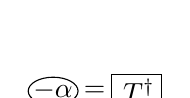
\begin{tikzpicture}[scale=1.000000,x=1pt,y=1pt]
\filldraw[color=white] (0.000000, -7.500000) rectangle (35.000000, 7.500000);
% Drawing wires
% Line 1: a W
%\draw[color=black] (0.000000,0.000000) -- (87.000000,0.000000);
% Done with wires; drawing gates
% Line 2: a P $-\alpha$ height=10 width=18
\begin{scope}
\draw[fill=white] (0.000000, 0.000000) ellipse(9.000000pt and 5.000000pt);
\clip (0.000000, 0.000000) ellipse(9.000000pt and 5.000000pt);
\draw (0.000000, 0.000000) node {$-\alpha$};
\end{scope}
% Line 3: =
%\draw[fill=white,color=white] (25.000000, -6.000000) rectangle (40.000000, 6.000000);
\draw (15.000000, 0.000000) node {$=$};
%% Line 4: a G $T^\dagger$ width=18
\begin{scope}
\draw[fill=white] (30.000000, -0.000000) +(-45.000000:12.727922pt and 8.485281pt) -- +(45.000000:12.727922pt and 8.485281pt) -- +(135.000000:12.727922pt and 8.485281pt) -- +(225.000000:12.727922pt and 8.485281pt) -- cycle;
\clip (30.000000, -0.000000) +(-45.000000:12.727922pt and 8.485281pt) -- +(45.000000:12.727922pt and 8.485281pt) -- +(135.000000:12.727922pt and 8.485281pt) -- +(225.000000:12.727922pt and 8.485281pt) -- cycle;
\draw (31.000000, -0.000000) node {$T^\dagger$};
\end{scope}
%% Done with gates; drawing ending labels
%% Done with ending labels; drawing cut lines and comments
%% Done with comments
\end{tikzpicture}
and
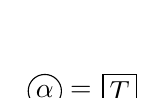
\begin{tikzpicture}[scale=1.000000,x=1pt,y=1pt]
\filldraw[color=white] (0.000000, -7.500000) rectangle (23.000000, 7.500000);
% Drawing wires
% Line 1: a W
%\draw[color=black] (0.000000,0.000000) -- (87.000000,0.000000);
% Done with wires; drawing gates
% Line 2: a P $-\alpha$ height=10 width=18
\begin{scope}
\draw[fill=white] (0.000000, 0.000000) circle(6.000000pt);
\clip (0.000000, 0.000000) circle(6.000000pt);
\draw (0.000000, 0.000000) node {$\alpha$};
\end{scope}
% Line 3: =
%\draw[fill=white,color=white] (25.000000, -6.000000) rectangle (40.000000, 6.000000);
\draw (13.000000, 0.000000) node {$=$};
%% Line 4: a G $T^\dagger$ width=18
\begin{scope}
\draw[fill=white] (27.000000, -0.000000) +(-45.000000:8.485281pt and 8.485281pt) -- +(45.000000:8.485281pt and 8.485281pt) -- +(135.000000:8.485281pt and 8.485281pt) -- +(225.000000:8.485281pt and 8.485281pt) -- cycle;
\clip (27.000000, -0.000000) +(-45.000000:8.485281pt and 8.485281pt) -- +(45.000000:8.485281pt and 8.485281pt) -- +(135.000000:8.485281pt and 8.485281pt) -- +(225.000000:8.485281pt and 8.485281pt) -- cycle;
\draw (27.000000, -0.000000) node {$T$};
\end{scope}
%% Done with gates; drawing ending labels
%% Done with ending labels; drawing cut lines and comments
%% Done with comments
\end{tikzpicture}.  So:
\begin{center}
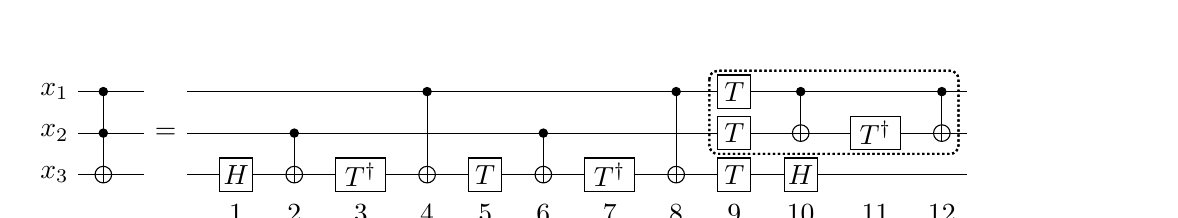
\begin{tikzpicture}[scale=1.000000,x=1pt,y=1pt]
\filldraw[color=white] (0.000000, -7.500000) rectangle (321.000000, 37.500000);
% Drawing wires
% Line 1: a3 W x_1
\draw[color=black] (0.000000,30.000000) -- (321.000000,30.000000);
\draw[color=black] (0.000000,30.000000) node[left] {$x_1$};
% Line 2: a2 W x_2
\draw[color=black] (0.000000,15.000000) -- (321.000000,15.000000);
\draw[color=black] (0.000000,15.000000) node[left] {$x_2$};
% Line 3: a1 W x_3
\draw[color=black] (0.000000,0.000000) -- (321.000000,0.000000);
\draw[color=black] (0.000000,0.000000) node[left] {$x_3$};
% Done with wires; drawing gates
% Line 4: +a1 a2 a3
\draw (9.000000,30.000000) -- (9.000000,0.000000);
\begin{scope}
\draw[fill=white] (9.000000, 0.000000) circle(3.000000pt);
\clip (9.000000, 0.000000) circle(3.000000pt);
\draw (6.000000, 0.000000) -- (12.000000, 0.000000);
\draw (9.000000, -3.000000) -- (9.000000, 3.000000);
\end{scope}
\filldraw (9.000000, 15.000000) circle(1.500000pt);
\filldraw (9.000000, 30.000000) circle(1.500000pt);
% Line 5: =
\draw[fill=white,color=white] (24.000000, -6.000000) rectangle (39.000000, 36.000000);
\draw (31.500000, 15.000000) node {$=$};
% Line 6: a1 H %% 1
\draw (57.000000, -7.500000) node[text width=144pt,below,text centered] {1};
\begin{scope}
\draw[fill=white] (57.000000, -0.000000) +(-45.000000:8.485281pt and 8.485281pt) -- +(45.000000:8.485281pt and 8.485281pt) -- +(135.000000:8.485281pt and 8.485281pt) -- +(225.000000:8.485281pt and 8.485281pt) -- cycle;
\clip (57.000000, -0.000000) +(-45.000000:8.485281pt and 8.485281pt) -- +(45.000000:8.485281pt and 8.485281pt) -- +(135.000000:8.485281pt and 8.485281pt) -- +(225.000000:8.485281pt and 8.485281pt) -- cycle;
\draw (57.000000, -0.000000) node {$H$};
\end{scope}
% Line 7: +a1 a2 %% 2
\draw (78.000000, -7.500000) node[text width=144pt,below,text centered] {2};
\draw (78.000000,15.000000) -- (78.000000,0.000000);
\begin{scope}
\draw[fill=white] (78.000000, 0.000000) circle(3.000000pt);
\clip (78.000000, 0.000000) circle(3.000000pt);
\draw (75.000000, 0.000000) -- (81.000000, 0.000000);
\draw (78.000000, -3.000000) -- (78.000000, 3.000000);
\end{scope}
\filldraw (78.000000, 15.000000) circle(1.500000pt);
% Line 8: a1 G $T^\dagger$ width=18 %% 3
\draw (102.000000, -7.500000) node[text width=144pt,below,text centered] {3};
\begin{scope}
\draw[fill=white] (102.000000, -0.000000) +(-45.000000:12.727922pt and 8.485281pt) -- +(45.000000:12.727922pt and 8.485281pt) -- +(135.000000:12.727922pt and 8.485281pt) -- +(225.000000:12.727922pt and 8.485281pt) -- cycle;
\clip (102.000000, -0.000000) +(-45.000000:12.727922pt and 8.485281pt) -- +(45.000000:12.727922pt and 8.485281pt) -- +(135.000000:12.727922pt and 8.485281pt) -- +(225.000000:12.727922pt and 8.485281pt) -- cycle;
\draw (102.000000, -0.000000) node {$T^\dagger$};
\end{scope}
% Line 9: +a1 a3 %% 4
\draw (126.000000, -7.500000) node[text width=144pt,below,text centered] {4};
\draw (126.000000,30.000000) -- (126.000000,0.000000);
\begin{scope}
\draw[fill=white] (126.000000, 0.000000) circle(3.000000pt);
\clip (126.000000, 0.000000) circle(3.000000pt);
\draw (123.000000, 0.000000) -- (129.000000, 0.000000);
\draw (126.000000, -3.000000) -- (126.000000, 3.000000);
\end{scope}
\filldraw (126.000000, 30.000000) circle(1.500000pt);
% Line 10: a1 G $T$ %% 5
\draw (147.000000, -7.500000) node[text width=144pt,below,text centered] {5};
\begin{scope}
\draw[fill=white] (147.000000, -0.000000) +(-45.000000:8.485281pt and 8.485281pt) -- +(45.000000:8.485281pt and 8.485281pt) -- +(135.000000:8.485281pt and 8.485281pt) -- +(225.000000:8.485281pt and 8.485281pt) -- cycle;
\clip (147.000000, -0.000000) +(-45.000000:8.485281pt and 8.485281pt) -- +(45.000000:8.485281pt and 8.485281pt) -- +(135.000000:8.485281pt and 8.485281pt) -- +(225.000000:8.485281pt and 8.485281pt) -- cycle;
\draw (147.000000, -0.000000) node {$T$};
\end{scope}
% Line 11: +a1 a2 %% 6
\draw (168.000000, -7.500000) node[text width=144pt,below,text centered] {6};
\draw (168.000000,15.000000) -- (168.000000,0.000000);
\begin{scope}
\draw[fill=white] (168.000000, 0.000000) circle(3.000000pt);
\clip (168.000000, 0.000000) circle(3.000000pt);
\draw (165.000000, 0.000000) -- (171.000000, 0.000000);
\draw (168.000000, -3.000000) -- (168.000000, 3.000000);
\end{scope}
\filldraw (168.000000, 15.000000) circle(1.500000pt);
% Line 12: a1 G $T^\dagger$ width=18 %% 7
\draw (192.000000, -7.500000) node[text width=144pt,below,text centered] {7};
\begin{scope}
\draw[fill=white] (192.000000, -0.000000) +(-45.000000:12.727922pt and 8.485281pt) -- +(45.000000:12.727922pt and 8.485281pt) -- +(135.000000:12.727922pt and 8.485281pt) -- +(225.000000:12.727922pt and 8.485281pt) -- cycle;
\clip (192.000000, -0.000000) +(-45.000000:12.727922pt and 8.485281pt) -- +(45.000000:12.727922pt and 8.485281pt) -- +(135.000000:12.727922pt and 8.485281pt) -- +(225.000000:12.727922pt and 8.485281pt) -- cycle;
\draw (192.000000, -0.000000) node {$T^\dagger$};
\end{scope}
% Line 13: +a1 a3 %% 8
\draw (216.000000, -7.500000) node[text width=144pt,below,text centered] {8};
\draw (216.000000,30.000000) -- (216.000000,0.000000);
\begin{scope}
\draw[fill=white] (216.000000, 0.000000) circle(3.000000pt);
\clip (216.000000, 0.000000) circle(3.000000pt);
\draw (213.000000, 0.000000) -- (219.000000, 0.000000);
\draw (216.000000, -3.000000) -- (216.000000, 3.000000);
\end{scope}
\filldraw (216.000000, 30.000000) circle(1.500000pt);
% Line 14: TOUCH
% Line 15: a3 G $T$
\begin{scope}
\draw[fill=white] (237.000000, 30.000000) +(-45.000000:8.485281pt and 8.485281pt) -- +(45.000000:8.485281pt and 8.485281pt) -- +(135.000000:8.485281pt and 8.485281pt) -- +(225.000000:8.485281pt and 8.485281pt) -- cycle;
\clip (237.000000, 30.000000) +(-45.000000:8.485281pt and 8.485281pt) -- +(45.000000:8.485281pt and 8.485281pt) -- +(135.000000:8.485281pt and 8.485281pt) -- +(225.000000:8.485281pt and 8.485281pt) -- cycle;
\draw (237.000000, 30.000000) node {$T$};
\end{scope}
% Line 16: a2 G $T$
\begin{scope}
\draw[fill=white] (237.000000, 15.000000) +(-45.000000:8.485281pt and 8.485281pt) -- +(45.000000:8.485281pt and 8.485281pt) -- +(135.000000:8.485281pt and 8.485281pt) -- +(225.000000:8.485281pt and 8.485281pt) -- cycle;
\clip (237.000000, 15.000000) +(-45.000000:8.485281pt and 8.485281pt) -- +(45.000000:8.485281pt and 8.485281pt) -- +(135.000000:8.485281pt and 8.485281pt) -- +(225.000000:8.485281pt and 8.485281pt) -- cycle;
\draw (237.000000, 15.000000) node {$T$};
\end{scope}
% Line 17: a1 G $T$ %% 9
\draw (237.000000, -7.500000) node[text width=144pt,below,text centered] {9};
\begin{scope}
\draw[fill=white] (237.000000, -0.000000) +(-45.000000:8.485281pt and 8.485281pt) -- +(45.000000:8.485281pt and 8.485281pt) -- +(135.000000:8.485281pt and 8.485281pt) -- +(225.000000:8.485281pt and 8.485281pt) -- cycle;
\clip (237.000000, -0.000000) +(-45.000000:8.485281pt and 8.485281pt) -- +(45.000000:8.485281pt and 8.485281pt) -- +(135.000000:8.485281pt and 8.485281pt) -- +(225.000000:8.485281pt and 8.485281pt) -- cycle;
\draw (237.000000, -0.000000) node {$T$};
\end{scope}
% Line 18: a1 H
\begin{scope}
\draw[fill=white] (261.000000, -0.000000) +(-45.000000:8.485281pt and 8.485281pt) -- +(45.000000:8.485281pt and 8.485281pt) -- +(135.000000:8.485281pt and 8.485281pt) -- +(225.000000:8.485281pt and 8.485281pt) -- cycle;
\clip (261.000000, -0.000000) +(-45.000000:8.485281pt and 8.485281pt) -- +(45.000000:8.485281pt and 8.485281pt) -- +(135.000000:8.485281pt and 8.485281pt) -- +(225.000000:8.485281pt and 8.485281pt) -- cycle;
\draw (261.000000, -0.000000) node {$H$};
\end{scope}
% Line 19: +a2 a3 %% 10
\draw (261.000000, -7.500000) node[text width=144pt,below,text centered] {10};
\draw (261.000000,30.000000) -- (261.000000,15.000000);
\begin{scope}
\draw[fill=white] (261.000000, 15.000000) circle(3.000000pt);
\clip (261.000000, 15.000000) circle(3.000000pt);
\draw (258.000000, 15.000000) -- (264.000000, 15.000000);
\draw (261.000000, 12.000000) -- (261.000000, 18.000000);
\end{scope}
\filldraw (261.000000, 30.000000) circle(1.500000pt);
% Line 20: a2 G $T^\dagger$ width=18 %% 11
\draw (288.000000, -7.500000) node[text width=144pt,below,text centered] {11};
\begin{scope}
\draw[fill=white] (288.000000, 15.000000) +(-45.000000:12.727922pt and 8.485281pt) -- +(45.000000:12.727922pt and 8.485281pt) -- +(135.000000:12.727922pt and 8.485281pt) -- +(225.000000:12.727922pt and 8.485281pt) -- cycle;
\clip (288.000000, 15.000000) +(-45.000000:12.727922pt and 8.485281pt) -- +(45.000000:12.727922pt and 8.485281pt) -- +(135.000000:12.727922pt and 8.485281pt) -- +(225.000000:12.727922pt and 8.485281pt) -- cycle;
\draw (288.000000, 15.000000) node {$T^\dagger$};
\end{scope}
% Line 21: +a2 a3 %% 12
\draw (312.000000, -7.500000) node[text width=144pt,below,text centered] {12};
\draw (312.000000,30.000000) -- (312.000000,15.000000);
\begin{scope}
\draw[fill=white] (312.000000, 15.000000) circle(3.000000pt);
\clip (312.000000, 15.000000) circle(3.000000pt);
\draw (309.000000, 15.000000) -- (315.000000, 15.000000);
\draw (312.000000, 12.000000) -- (312.000000, 18.000000);
\end{scope}
\filldraw (312.000000, 30.000000) circle(1.500000pt);
% Done with gates; drawing ending labels
% Done with ending labels; drawing cut lines and comments
% Line 22: a3 a2 @  4 color=black style=densely_dotted,thick,rounded_corners=3pt
\draw[draw opacity=1.000000,fill opacity=0.200000,color=black,densely dotted,thick,rounded corners=3pt] (228.000000,37.500000) rectangle (318.000000,7.500000);
\draw[draw opacity=1.000000,fill opacity=0.200000,color=black,densely dotted,thick,rounded corners=3pt] (228.000000,37.500000) rectangle (318.000000,7.500000);
% Done with comments
\end{tikzpicture}
\end{center}
\vspace{-10pt}
All that remains is to show that the grouped subcircuits are equivalent, that is, to show that
\begin{center}
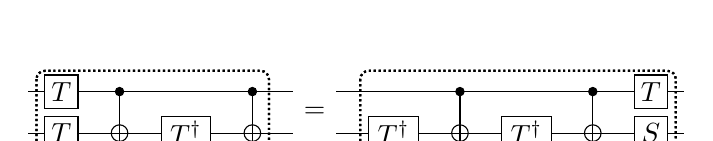
\begin{tikzpicture}[scale=1.000000,x=1pt,y=1pt]
\filldraw[color=white] (0.000000, -7.500000) rectangle (237.000000, 22.500000);
% Drawing wires
% Line 1: a2 W
\draw[color=black] (0.000000,15.000000) -- (237.000000,15.000000);
% Line 2: a1 W
\draw[color=black] (0.000000,0.000000) -- (237.000000,0.000000);
% Done with wires; drawing gates
% Line 3: a2 G $T$
\begin{scope}
\draw[fill=white] (12.000000, 15.000000) +(-45.000000:8.485281pt and 8.485281pt) -- +(45.000000:8.485281pt and 8.485281pt) -- +(135.000000:8.485281pt and 8.485281pt) -- +(225.000000:8.485281pt and 8.485281pt) -- cycle;
\clip (12.000000, 15.000000) +(-45.000000:8.485281pt and 8.485281pt) -- +(45.000000:8.485281pt and 8.485281pt) -- +(135.000000:8.485281pt and 8.485281pt) -- +(225.000000:8.485281pt and 8.485281pt) -- cycle;
\draw (12.000000, 15.000000) node {$T$};
\end{scope}
% Line 4: a1 G $T$
\begin{scope}
\draw[fill=white] (12.000000, -0.000000) +(-45.000000:8.485281pt and 8.485281pt) -- +(45.000000:8.485281pt and 8.485281pt) -- +(135.000000:8.485281pt and 8.485281pt) -- +(225.000000:8.485281pt and 8.485281pt) -- cycle;
\clip (12.000000, -0.000000) +(-45.000000:8.485281pt and 8.485281pt) -- +(45.000000:8.485281pt and 8.485281pt) -- +(135.000000:8.485281pt and 8.485281pt) -- +(225.000000:8.485281pt and 8.485281pt) -- cycle;
\draw (12.000000, -0.000000) node {$T$};
\end{scope}
% Line 5: +a1 a2
\draw (33.000000,15.000000) -- (33.000000,0.000000);
\begin{scope}
\draw[fill=white] (33.000000, 0.000000) circle(3.000000pt);
\clip (33.000000, 0.000000) circle(3.000000pt);
\draw (30.000000, 0.000000) -- (36.000000, 0.000000);
\draw (33.000000, -3.000000) -- (33.000000, 3.000000);
\end{scope}
\filldraw (33.000000, 15.000000) circle(1.500000pt);
% Line 6: a1 G $T^\dagger$ width=18
\begin{scope}
\draw[fill=white] (57.000000, -0.000000) +(-45.000000:12.727922pt and 8.485281pt) -- +(45.000000:12.727922pt and 8.485281pt) -- +(135.000000:12.727922pt and 8.485281pt) -- +(225.000000:12.727922pt and 8.485281pt) -- cycle;
\clip (57.000000, -0.000000) +(-45.000000:12.727922pt and 8.485281pt) -- +(45.000000:12.727922pt and 8.485281pt) -- +(135.000000:12.727922pt and 8.485281pt) -- +(225.000000:12.727922pt and 8.485281pt) -- cycle;
\draw (57.000000, -0.000000) node {$T^\dagger$};
\end{scope}
% Line 7: +a1 a2
\draw (81.000000,15.000000) -- (81.000000,0.000000);
\begin{scope}
\draw[fill=white] (81.000000, 0.000000) circle(3.000000pt);
\clip (81.000000, 0.000000) circle(3.000000pt);
\draw (78.000000, 0.000000) -- (84.000000, 0.000000);
\draw (81.000000, -3.000000) -- (81.000000, 3.000000);
\end{scope}
\filldraw (81.000000, 15.000000) circle(1.500000pt);
% Line 9: =
\draw[fill=white,color=white] (96.000000, -6.000000) rectangle (111.000000, 21.000000);
\draw (103.500000, 7.500000) node {$=$};
% Line 10: a1 G $T^\dagger$ width=18
\begin{scope}
\draw[fill=white] (132.000000, -0.000000) +(-45.000000:12.727922pt and 8.485281pt) -- +(45.000000:12.727922pt and 8.485281pt) -- +(135.000000:12.727922pt and 8.485281pt) -- +(225.000000:12.727922pt and 8.485281pt) -- cycle;
\clip (132.000000, -0.000000) +(-45.000000:12.727922pt and 8.485281pt) -- +(45.000000:12.727922pt and 8.485281pt) -- +(135.000000:12.727922pt and 8.485281pt) -- +(225.000000:12.727922pt and 8.485281pt) -- cycle;
\draw (132.000000, -0.000000) node {$T^\dagger$};
\end{scope}
% Line 11: +a1 a2
\draw (156.000000,15.000000) -- (156.000000,0.000000);
\begin{scope}
\draw[fill=white] (156.000000, 0.000000) circle(3.000000pt);
\clip (156.000000, 0.000000) circle(3.000000pt);
\draw (153.000000, 0.000000) -- (159.000000, 0.000000);
\draw (156.000000, -3.000000) -- (156.000000, 3.000000);
\end{scope}
\filldraw (156.000000, 15.000000) circle(1.500000pt);
% Line 12: a1 G $T^\dagger$ width=18
\begin{scope}
\draw[fill=white] (180.000000, -0.000000) +(-45.000000:12.727922pt and 8.485281pt) -- +(45.000000:12.727922pt and 8.485281pt) -- +(135.000000:12.727922pt and 8.485281pt) -- +(225.000000:12.727922pt and 8.485281pt) -- cycle;
\clip (180.000000, -0.000000) +(-45.000000:12.727922pt and 8.485281pt) -- +(45.000000:12.727922pt and 8.485281pt) -- +(135.000000:12.727922pt and 8.485281pt) -- +(225.000000:12.727922pt and 8.485281pt) -- cycle;
\draw (180.000000, -0.000000) node {$T^\dagger$};
\end{scope}
% Line 13: +a1 a2
\draw (204.000000,15.000000) -- (204.000000,0.000000);
\begin{scope}
\draw[fill=white] (204.000000, 0.000000) circle(3.000000pt);
\clip (204.000000, 0.000000) circle(3.000000pt);
\draw (201.000000, 0.000000) -- (207.000000, 0.000000);
\draw (204.000000, -3.000000) -- (204.000000, 3.000000);
\end{scope}
\filldraw (204.000000, 15.000000) circle(1.500000pt);
% Line 14: a2 G $T$
\begin{scope}
\draw[fill=white] (225.000000, 15.000000) +(-45.000000:8.485281pt and 8.485281pt) -- +(45.000000:8.485281pt and 8.485281pt) -- +(135.000000:8.485281pt and 8.485281pt) -- +(225.000000:8.485281pt and 8.485281pt) -- cycle;
\clip (225.000000, 15.000000) +(-45.000000:8.485281pt and 8.485281pt) -- +(45.000000:8.485281pt and 8.485281pt) -- +(135.000000:8.485281pt and 8.485281pt) -- +(225.000000:8.485281pt and 8.485281pt) -- cycle;
\draw (225.000000, 15.000000) node {$T$};
\end{scope}
% Line 15: a1 G $S$
\begin{scope}
\draw[fill=white] (225.000000, -0.000000) +(-45.000000:8.485281pt and 8.485281pt) -- +(45.000000:8.485281pt and 8.485281pt) -- +(135.000000:8.485281pt and 8.485281pt) -- +(225.000000:8.485281pt and 8.485281pt) -- cycle;
\clip (225.000000, -0.000000) +(-45.000000:8.485281pt and 8.485281pt) -- +(45.000000:8.485281pt and 8.485281pt) -- +(135.000000:8.485281pt and 8.485281pt) -- +(225.000000:8.485281pt and 8.485281pt) -- cycle;
\draw (225.000000, -0.000000) node {$S$};
\end{scope}
% Done with gates; drawing ending labels
% Done with ending labels; drawing cut lines and comments
% Line 8: a2 a1 @  4 color=black style=densely_dotted,thick,rounded_corners=3pt
\draw[draw opacity=1.000000,fill opacity=0.200000,color=black,densely dotted,thick,rounded corners=3pt] (3.000000,22.500000) rectangle (87.000000,-7.500000);
\draw[draw opacity=1.000000,fill opacity=0.200000,color=black,densely dotted,thick,rounded corners=3pt] (3.000000,22.500000) rectangle (87.000000,-7.500000);
% Line 16: a2 a1 @  5 color=black style=densely_dotted,thick,rounded_corners=3pt
\draw[draw opacity=1.000000,fill opacity=0.200000,color=black,densely dotted,thick,rounded corners=3pt] (120.000000,22.500000) rectangle (234.000000,-7.500000);
\draw[draw opacity=1.000000,fill opacity=0.200000,color=black,densely dotted,thick,rounded corners=3pt] (120.000000,22.500000) rectangle (234.000000,-7.500000);
% Done with comments
\end{tikzpicture}
\end{center}
\vspace{-10pt}
We do this by matrix mutiplication.  On the left, we have:
$$\begin{bmatrix} 1 & 0 & 0 &0 \\ 0 & 1 & 0 & 0 \\ 0 & 0 & 0 & 1 \\ 0 & 0 & 1 & 0\end{bmatrix}
\begin{bmatrix} 1 & 0 & 0 &0 \\ 0 & e^{-i\pi/4} & 0 & 0 \\ 0 & 0 & 1 & 0 \\ 0 & 0 & 0 & e^{-i\pi/4}\end{bmatrix}
\begin{bmatrix} 1 & 0 & 0 &0 \\ 0 & 1 & 0 & 0 \\ 0 & 0 & 0 & 1 \\ 0 & 0 & 1 & 0\end{bmatrix}
\begin{bmatrix} 1 & 0 & 0 &0 \\ 0 & 1 & 0 & 0 \\ 0 & 0 & e^{i\pi/4} & 0 \\ 0 & 0 & 0 & e^{i\pi/4}\end{bmatrix}
\begin{bmatrix} 1 & 0 & 0 &0 \\ 0 & e^{i\pi/4} & 0 & 0 \\ 0 & 0 & 1 & 0 \\ 0 & 0 & 0 & e^{i\pi/4}\end{bmatrix}$$
$$ = \begin{bmatrix} 1 & 0 & 0 &0 \\ 0 & 1 & 0 & 0 \\ 0 & 0 & 1 & 0 \\ 0 & 0 & 0 & i\end{bmatrix}$$
On the right:
$$
\begin{bmatrix} 1 & 0 & 0 &0 \\ 0 & i & 0 & 0 \\ 0 & 0 & 1 & 0 \\ 0 & 0 & 0 & i\end{bmatrix}
\begin{bmatrix} 1 & 0 & 0 &0 \\ 0 & 1 & 0 & 0 \\ 0 & 0 & e^{i\pi/4} & 0 \\ 0 & 0 & 0 & e^{i\pi/4}\end{bmatrix}
\begin{bmatrix} 1 & 0 & 0 &0 \\ 0 & 1 & 0 & 0 \\ 0 & 0 & 0 & 1 \\ 0 & 0 & 1 & 0\end{bmatrix}
\begin{bmatrix} 1 & 0 & 0 &0 \\ 0 & e^{-i\pi/4} & 0 & 0 \\ 0 & 0 & 1 & 0 \\ 0 & 0 & 0 & e^{-i\pi/4}\end{bmatrix}
\begin{bmatrix} 1 & 0 & 0 &0 \\ 0 & 1 & 0 & 0 \\ 0 & 0 & 0 & 1 \\ 0 & 0 & 1 & 0\end{bmatrix}\ \ \ \ \setminus$$
$$\cdot\begin{bmatrix} 1 & 0 & 0 &0 \\ 0 & e^{-i\pi/4} & 0 & 0 \\ 0 & 0 & 1 & 0 \\ 0 & 0 & 0 & e^{-i\pi/4}\end{bmatrix} = \begin{bmatrix} 1 & 0 & 0 &0 \\ 0 & 1 & 0 & 0 \\ 0 & 0 & 1 & 0 \\ 0 & 0 & 0 & i\end{bmatrix}$$
So, the subcircuits are equivalent and Figure 4.9 implements the Toffoli gate.  Note that both subcircuits execute a controlled-$S$ gate on $\ket{x_2}$, controlled by $\ket{x_1}$,  The subcircuit in the construction provided by the exercise is the result of a direct application of Figure 6, where $A=S, B=C=T^\dagger$, and $\alpha =\pi/4$, since $ABC=S(T^\dagger)^2=SS^\dagger=I$, and $e^{i\alpha}AXBXC=e^{i\pi/4}SXT^\dagger XT^\dagger= S$ can be easily verified via matrix-multiplication

\Textbf{4.25} Recall that the Fredkin (controlled-swap) gate performs the transform
$$\begin{bmatrix}
1 & 0 & 0 & 0 & 0 & 0 & 0 & 0 \\
0 & 1 & 0 & 0 & 0 & 0 & 0 & 0 \\
0 & 0 & 1 & 0 & 0 & 0 & 0 & 0 \\
0 & 0 & 0 & 1 & 0 & 0 & 0 & 0 \\
0 & 0 & 0 & 0 & 1 & 0 & 0 & 0 \\
0 & 0 & 0 & 0 & 0 & 0 & 1 & 0 \\
0 & 0 & 0 & 0 & 0 & 1 & 0 & 0 \\
0 & 0 & 0 & 0 & 0 & 0 & 0 & 1 
\end{bmatrix}$$
\begin{enumerate}
\item Give a quantum circuit which uses three Toffoli gates to construct the Fredkin gate (\textit{Hint:} think of the swap gate construction - you can control each gate one at a time)
\item Show that the first and last Toffoli gates can be replaced by \CNOT\ gates.
\item Now replace the middle Toffoli gate with the circuit in Figure 4.8 to obtain a Fredkin gate construction using only six two-qubit gates
\item Can you come up with an even simpler construction, with only five two-qubit gates?
\end{enumerate}
\vspace{-15pt}
\Soln For part 1, we'll show the following circuit identity by tracing the result of each computational basis state through each of the three Toffolis, indexed 1-3.
\begin{center}\ \ \ \ \ \ \ \ \ \ \ \ \ \ 
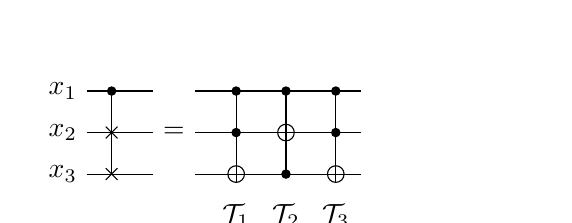
\begin{tikzpicture}[scale=1.000000,x=1pt,y=1pt]
\filldraw[color=white] (0.000000, -7.500000) rectangle (99.000000, 37.500000);
% Drawing wires
% Line 1: a3 W x_3
\draw[color=black] (0.000000,30.000000) -- (99.000000,30.000000);
\draw[color=black] (0.000000,30.000000) node[left] {$x_1$};
% Line 2: a2 W x_2
\draw[color=black] (0.000000,15.000000) -- (99.000000,15.000000);
\draw[color=black] (0.000000,15.000000) node[left] {$x_2$};
% Line 3: a1 W x_1
\draw[color=black] (0.000000,0.000000) -- (99.000000,0.000000);
\draw[color=black] (0.000000,0.000000) node[left] {$x_3$};
% Done with wires; drawing gates
% Line 4: a1 a2 SWAP a3
\draw (9.000000,30.000000) -- (9.000000,0.000000);
\begin{scope}
\draw (6.878680, -2.121320) -- (11.121320, 2.121320);
\draw (6.878680, 2.121320) -- (11.121320, -2.121320);
\end{scope}
\begin{scope}
\draw (6.878680, 12.878680) -- (11.121320, 17.121320);
\draw (6.878680, 17.121320) -- (11.121320, 12.878680);
\end{scope}
\filldraw (9.000000, 30.000000) circle(1.500000pt);
% Line 5: =
\draw[fill=white,color=white] (24.000000, -6.000000) rectangle (39.000000, 36.000000);
\draw (31.500000, 15.000000) node {$=$};
% Line 6: a1 T a2 a3 %% $\mathcal{T}_1$
\draw (54.000000, -7.500000) node[text width=144pt,below,text centered] {$\mathcal{T}_1$};
\draw (54.000000,30.000000) -- (54.000000,0.000000);
\begin{scope}
\draw[fill=white] (54.000000, 0.000000) circle(3.000000pt);
\clip (54.000000, 0.000000) circle(3.000000pt);
\draw (51.000000, 0.000000) -- (57.000000, 0.000000);
\draw (54.000000, -3.000000) -- (54.000000, 3.000000);
\end{scope}
\filldraw (54.000000, 15.000000) circle(1.500000pt);
\filldraw (54.000000, 30.000000) circle(1.500000pt);
% Line 7: a2 T a1 a3 %% $\mathcal{T}_2$
\draw (72.000000, -7.500000) node[text width=144pt,below,text centered] {$\mathcal{T}_2$};
\draw (72.000000,30.000000) -- (72.000000,0.000000);
\begin{scope}
\draw[fill=white] (72.000000, 15.000000) circle(3.000000pt);
\clip (72.000000, 15.000000) circle(3.000000pt);
\draw (69.000000, 15.000000) -- (75.000000, 15.000000);
\draw (72.000000, 12.000000) -- (72.000000, 18.000000);
\end{scope}
\filldraw (72.000000, 0.000000) circle(1.500000pt);
\filldraw (72.000000, 30.000000) circle(1.500000pt);
% Line 8: a1 T a2 a3 %% $\mathcal{T}_3$
\draw (90.000000, -7.500000) node[text width=144pt,below,text centered] {$\mathcal{T}_3$};
\draw (90.000000,30.000000) -- (90.000000,0.000000);
\begin{scope}
\draw[fill=white] (90.000000, 0.000000) circle(3.000000pt);
\clip (90.000000, 0.000000) circle(3.000000pt);
\draw (87.000000, 0.000000) -- (93.000000, 0.000000);
\draw (90.000000, -3.000000) -- (90.000000, 3.000000);
\end{scope}
\filldraw (90.000000, 15.000000) circle(1.500000pt);
\filldraw (90.000000, 30.000000) circle(1.500000pt);
% Done with gates; drawing ending labels
% Done with ending labels; drawing cut lines and comments
% Done with comments
\end{tikzpicture}
\end{center}
\vspace{-10pt}
\begin{center}
\begin{tabular}{c|c|c|c|} 
$\ket{x_1x_2x_3}$ & $\mathcal{T}_1$ & $\mathcal{T}_2$ & $\mathcal{T}_3$ \\
\hline
$\ket{000}$ & $\ket{000}$ & $\ket{000}$ & $\ket{000}$  \\
\hline
$\ket{001}$  & $\ket{001}$ & $\ket{001}$ & $\ket{001}$ \\
\hline
$\ket{010}$ & $\ket{010}$ & $\ket{010}$ & $\ket{010}$ \\
\hline
$\ket{011}$& $\ket{011}$ & $\ket{011}$ & $\ket{011}$ \\
\hline
$\ket{100}$ & $\ket{100}$ & $\ket{100}$ & $\ket{100}$ \\
\hline
$\ket{101}$ & $\ket{101}$ & $\ket{111}$ & $\ket{110}$ \\
\hline
$\ket{110}$ & $\ket{111}$ & $\ket{101}$ & $\ket{101}$ \\
\hline
$\ket{111}$ & $\ket{110}$ & $\ket{110}$ & $\ket{111}$ 
\end{tabular}
\end{center}
\vspace{-10pt}
For part 2, we replace $\mathcal{T}_1$ and $\mathcal{T}_3$ with \CNOT$(x_2, x_3)$.
\begin{center}\ \ \ \ \ \ \ \ \ \ \ \ \ \ 
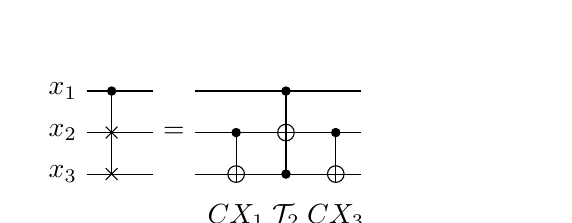
\begin{tikzpicture}[scale=1.000000,x=1pt,y=1pt]
\filldraw[color=white] (0.000000, -7.500000) rectangle (99.000000, 37.500000);
% Drawing wires
% Line 1: a3 W x_1
\draw[color=black] (0.000000,30.000000) -- (99.000000,30.000000);
\draw[color=black] (0.000000,30.000000) node[left] {$x_1$};
% Line 2: a2 W x_2
\draw[color=black] (0.000000,15.000000) -- (99.000000,15.000000);
\draw[color=black] (0.000000,15.000000) node[left] {$x_2$};
% Line 3: a1 W x_3
\draw[color=black] (0.000000,0.000000) -- (99.000000,0.000000);
\draw[color=black] (0.000000,0.000000) node[left] {$x_3$};
% Done with wires; drawing gates
% Line 4: a1 a2 SWAP a3
\draw (9.000000,30.000000) -- (9.000000,0.000000);
\begin{scope}
\draw (6.878680, -2.121320) -- (11.121320, 2.121320);
\draw (6.878680, 2.121320) -- (11.121320, -2.121320);
\end{scope}
\begin{scope}
\draw (6.878680, 12.878680) -- (11.121320, 17.121320);
\draw (6.878680, 17.121320) -- (11.121320, 12.878680);
\end{scope}
\filldraw (9.000000, 30.000000) circle(1.500000pt);
% Line 5: =
\draw[fill=white,color=white] (24.000000, -6.000000) rectangle (39.000000, 36.000000);
\draw (31.500000, 15.000000) node {$=$};
% Line 6: +a1 a2 %% $CX_1$
\draw (54.000000, -7.500000) node[text width=144pt,below,text centered] {$CX_1$};
\draw (54.000000,15.000000) -- (54.000000,0.000000);
\begin{scope}
\draw[fill=white] (54.000000, 0.000000) circle(3.000000pt);
\clip (54.000000, 0.000000) circle(3.000000pt);
\draw (51.000000, 0.000000) -- (57.000000, 0.000000);
\draw (54.000000, -3.000000) -- (54.000000, 3.000000);
\end{scope}
\filldraw (54.000000, 15.000000) circle(1.500000pt);
% Line 7: a2 T a1 a3 %% $\mathcal{T}_2$
\draw (72.000000, -7.500000) node[text width=144pt,below,text centered] {$\mathcal{T}_2$};
\draw (72.000000,30.000000) -- (72.000000,0.000000);
\begin{scope}
\draw[fill=white] (72.000000, 15.000000) circle(3.000000pt);
\clip (72.000000, 15.000000) circle(3.000000pt);
\draw (69.000000, 15.000000) -- (75.000000, 15.000000);
\draw (72.000000, 12.000000) -- (72.000000, 18.000000);
\end{scope}
\filldraw (72.000000, 0.000000) circle(1.500000pt);
\filldraw (72.000000, 30.000000) circle(1.500000pt);
% Line 8: +a1 a2 %% $CX_3$
\draw (90.000000, -7.500000) node[text width=144pt,below,text centered] {$CX_3$};
\draw (90.000000,15.000000) -- (90.000000,0.000000);
\begin{scope}
\draw[fill=white] (90.000000, 0.000000) circle(3.000000pt);
\clip (90.000000, 0.000000) circle(3.000000pt);
\draw (87.000000, 0.000000) -- (93.000000, 0.000000);
\draw (90.000000, -3.000000) -- (90.000000, 3.000000);
\end{scope}
\filldraw (90.000000, 15.000000) circle(1.500000pt);
% Done with gates; drawing ending labels
% Done with ending labels; drawing cut lines and comments
% Done with comments
\end{tikzpicture}
\end{center}
\vspace{-10pt}
\begin{center}
\begin{tabular}{c|c|c|c|} 
$\ket{x_1x_2x_3}$ & $CX_1$ & $\mathcal{T}_2$ & $CX_3$ \\
\hline
$\ket{000}$ & $\ket{000}$ & $\ket{000}$ & $\ket{000}$  \\
\hline
$\ket{001}$  & $\ket{001}$ & $\ket{001}$ & $\ket{001}$ \\
\hline
$\ket{010}$ & $\ket{011}$ & $\ket{011}$ & $\ket{010}$ \\
\hline
$\ket{011}$& $\ket{010}$ & $\ket{010}$ & $\ket{011}$ \\
\hline
$\ket{100}$ & $\ket{100}$ & $\ket{100}$ & $\ket{100}$ \\
\hline
$\ket{101}$ & $\ket{101}$ & $\ket{111}$ & $\ket{110}$ \\
\hline
$\ket{110}$ & $\ket{111}$ & $\ket{101}$ & $\ket{101}$ \\
\hline
$\ket{111}$ & $\ket{110}$ & $\ket{110}$ & $\ket{111}$ 
\end{tabular}
\end{center}
\vspace{-5pt}

For part 3, we rearrange $x_2$ and $x_3$.  To apply Figure 4.8 we let $U=X$, so that if $V=\frac{1-i}{2}(I+iX)$, then $V^2=X=U$, and we obtain
\begin{center}\ \ \ \ \ \ \ \ \ \ \ \ \ \ 
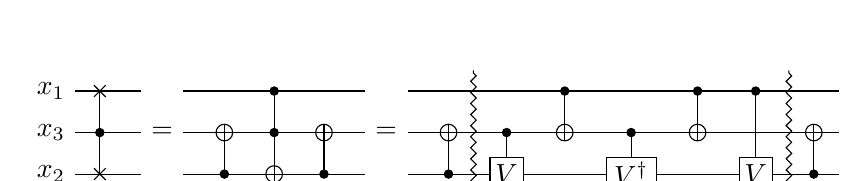
\begin{tikzpicture}[scale=1.000000,x=1pt,y=1pt]
\filldraw[color=white] (0.000000, -7.500000) rectangle (276.000000, 37.500000);
% Drawing wires
% Line 1: a3 W x_1
\draw[color=black] (0.000000,30.000000) -- (276.000000,30.000000);
\draw[color=black] (0.000000,30.000000) node[left] {$x_1$};
% Line 2: a2 W x_3
\draw[color=black] (0.000000,15.000000) -- (276.000000,15.000000);
\draw[color=black] (0.000000,15.000000) node[left] {$x_3$};
% Line 3: a1 W x_2
\draw[color=black] (0.000000,0.000000) -- (276.000000,0.000000);
\draw[color=black] (0.000000,0.000000) node[left] {$x_2$};
% Done with wires; drawing gates
% Line 4: a1 a3 SWAP a2
\draw (9.000000,30.000000) -- (9.000000,0.000000);
\begin{scope}
\draw (6.878680, -2.121320) -- (11.121320, 2.121320);
\draw (6.878680, 2.121320) -- (11.121320, -2.121320);
\end{scope}
\begin{scope}
\draw (6.878680, 27.878680) -- (11.121320, 32.121320);
\draw (6.878680, 32.121320) -- (11.121320, 27.878680);
\end{scope}
\filldraw (9.000000, 15.000000) circle(1.500000pt);
% Line 5: =
\draw[fill=white,color=white] (24.000000, -6.000000) rectangle (39.000000, 36.000000);
\draw (31.500000, 15.000000) node {$=$};
% Line 6: a1 +a2
\draw (54.000000,15.000000) -- (54.000000,0.000000);
\filldraw (54.000000, 0.000000) circle(1.500000pt);
\begin{scope}
\draw[fill=white] (54.000000, 15.000000) circle(3.000000pt);
\clip (54.000000, 15.000000) circle(3.000000pt);
\draw (51.000000, 15.000000) -- (57.000000, 15.000000);
\draw (54.000000, 12.000000) -- (54.000000, 18.000000);
\end{scope}
% Line 7: +a1 a2 a3
\draw (72.000000,30.000000) -- (72.000000,0.000000);
\begin{scope}
\draw[fill=white] (72.000000, 0.000000) circle(3.000000pt);
\clip (72.000000, 0.000000) circle(3.000000pt);
\draw (69.000000, 0.000000) -- (75.000000, 0.000000);
\draw (72.000000, -3.000000) -- (72.000000, 3.000000);
\end{scope}
\filldraw (72.000000, 15.000000) circle(1.500000pt);
\filldraw (72.000000, 30.000000) circle(1.500000pt);
% Line 8: a1 +a2
\draw (90.000000,15.000000) -- (90.000000,0.000000);
\filldraw (90.000000, 0.000000) circle(1.500000pt);
\begin{scope}
\draw[fill=white] (90.000000, 15.000000) circle(3.000000pt);
\clip (90.000000, 15.000000) circle(3.000000pt);
\draw (87.000000, 15.000000) -- (93.000000, 15.000000);
\draw (90.000000, 12.000000) -- (90.000000, 18.000000);
\end{scope}
% Line 9: =
\draw[fill=white,color=white] (105.000000, -6.000000) rectangle (120.000000, 36.000000);
\draw (112.500000, 15.000000) node {$=$};
% Line 10: a1 +a2
\draw (135.000000,15.000000) -- (135.000000,0.000000);
\filldraw (135.000000, 0.000000) circle(1.500000pt);
\begin{scope}
\draw[fill=white] (135.000000, 15.000000) circle(3.000000pt);
\clip (135.000000, 15.000000) circle(3.000000pt);
\draw (132.000000, 15.000000) -- (138.000000, 15.000000);
\draw (135.000000, 12.000000) -- (135.000000, 18.000000);
\end{scope}
% Line 11: BARRIER
\draw[decorate,decoration={zigzag,amplitude=1pt,segment length=4}] (144.000000,-7.500000) -- (144.000000,37.500000);
% Line 12: a1 G $V$ a2
\draw (156.000000,15.000000) -- (156.000000,0.000000);
\begin{scope}
\draw[fill=white] (156.000000, -0.000000) +(-45.000000:8.485281pt and 8.485281pt) -- +(45.000000:8.485281pt and 8.485281pt) -- +(135.000000:8.485281pt and 8.485281pt) -- +(225.000000:8.485281pt and 8.485281pt) -- cycle;
\clip (156.000000, -0.000000) +(-45.000000:8.485281pt and 8.485281pt) -- +(45.000000:8.485281pt and 8.485281pt) -- +(135.000000:8.485281pt and 8.485281pt) -- +(225.000000:8.485281pt and 8.485281pt) -- cycle;
\draw (156.000000, -0.000000) node {$V$};
\end{scope}
\filldraw (156.000000, 15.000000) circle(1.500000pt);
% Line 13: a3 +a2
\draw (177.000000,30.000000) -- (177.000000,15.000000);
\filldraw (177.000000, 30.000000) circle(1.500000pt);
\begin{scope}
\draw[fill=white] (177.000000, 15.000000) circle(3.000000pt);
\clip (177.000000, 15.000000) circle(3.000000pt);
\draw (174.000000, 15.000000) -- (180.000000, 15.000000);
\draw (177.000000, 12.000000) -- (177.000000, 18.000000);
\end{scope}
% Line 14: a1 G $V^\dagger$ a2 width=18
\draw (201.000000,15.000000) -- (201.000000,0.000000);
\begin{scope}
\draw[fill=white] (201.000000, -0.000000) +(-45.000000:12.727922pt and 8.485281pt) -- +(45.000000:12.727922pt and 8.485281pt) -- +(135.000000:12.727922pt and 8.485281pt) -- +(225.000000:12.727922pt and 8.485281pt) -- cycle;
\clip (201.000000, -0.000000) +(-45.000000:12.727922pt and 8.485281pt) -- +(45.000000:12.727922pt and 8.485281pt) -- +(135.000000:12.727922pt and 8.485281pt) -- +(225.000000:12.727922pt and 8.485281pt) -- cycle;
\draw (201.000000, -0.000000) node {$V^\dagger$};
\end{scope}
\filldraw (201.000000, 15.000000) circle(1.500000pt);
% Line 15: a3 +a2
\draw (225.000000,30.000000) -- (225.000000,15.000000);
\filldraw (225.000000, 30.000000) circle(1.500000pt);
\begin{scope}
\draw[fill=white] (225.000000, 15.000000) circle(3.000000pt);
\clip (225.000000, 15.000000) circle(3.000000pt);
\draw (222.000000, 15.000000) -- (228.000000, 15.000000);
\draw (225.000000, 12.000000) -- (225.000000, 18.000000);
\end{scope}
% Line 16: a1 G $V$ a3
\draw (246.000000,30.000000) -- (246.000000,0.000000);
\begin{scope}
\draw[fill=white] (246.000000, -0.000000) +(-45.000000:8.485281pt and 8.485281pt) -- +(45.000000:8.485281pt and 8.485281pt) -- +(135.000000:8.485281pt and 8.485281pt) -- +(225.000000:8.485281pt and 8.485281pt) -- cycle;
\clip (246.000000, -0.000000) +(-45.000000:8.485281pt and 8.485281pt) -- +(45.000000:8.485281pt and 8.485281pt) -- +(135.000000:8.485281pt and 8.485281pt) -- +(225.000000:8.485281pt and 8.485281pt) -- cycle;
\draw (246.000000, -0.000000) node {$V$};
\end{scope}
\filldraw (246.000000, 30.000000) circle(1.500000pt);
% Line 17: BARRIER
\draw[decorate,decoration={zigzag,amplitude=1pt,segment length=4}] (258.000000,-7.500000) -- (258.000000,37.500000);
% Line 18: a1 +a2
\draw (267.000000,15.000000) -- (267.000000,0.000000);
\filldraw (267.000000, 0.000000) circle(1.500000pt);
\begin{scope}
\draw[fill=white] (267.000000, 15.000000) circle(3.000000pt);
\clip (267.000000, 15.000000) circle(3.000000pt);
\draw (264.000000, 15.000000) -- (270.000000, 15.000000);
\draw (267.000000, 12.000000) -- (267.000000, 18.000000);
\end{scope}
% Done with gates; drawing ending labels
% Done with ending labels; drawing cut lines and comments
% Done with comments
\end{tikzpicture}
\end{center}
\vspace{-10pt}
This circuit contains 7 2-qubit gates, but consecutive applications of any 2-qubit gates to the same pair of qubits can be combined.  The resulting 2-qubit gate can likely not be thought of a  simple unitary applied to one of the qubits, controlled by the other though.  Still, combining the first two gates into a 2-qubit gate, say $G$, gives
\vspace{-5pt}
\begin{center}
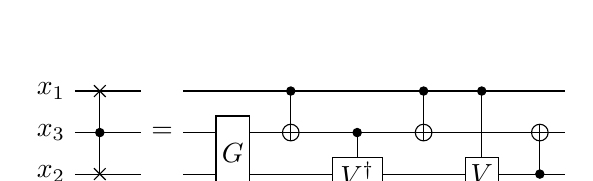
\begin{tikzpicture}[scale=1.000000,x=1pt,y=1pt]
\filldraw[color=white] (0.000000, -7.500000) rectangle (177.000000, 37.500000);
% Drawing wires
% Line 1: a3 W x_1
\draw[color=black] (0.000000,30.000000) -- (177.000000,30.000000);
\draw[color=black] (0.000000,30.000000) node[left] {$x_1$};
% Line 2: a2 W x_3
\draw[color=black] (0.000000,15.000000) -- (177.000000,15.000000);
\draw[color=black] (0.000000,15.000000) node[left] {$x_3$};
% Line 3: a1 W x_2
\draw[color=black] (0.000000,0.000000) -- (177.000000,0.000000);
\draw[color=black] (0.000000,0.000000) node[left] {$x_2$};
% Done with wires; drawing gates
% Line 4: a1 a3 SWAP a2
\draw (9.000000,30.000000) -- (9.000000,0.000000);
\begin{scope}
\draw (6.878680, -2.121320) -- (11.121320, 2.121320);
\draw (6.878680, 2.121320) -- (11.121320, -2.121320);
\end{scope}
\begin{scope}
\draw (6.878680, 27.878680) -- (11.121320, 32.121320);
\draw (6.878680, 32.121320) -- (11.121320, 27.878680);
\end{scope}
\filldraw (9.000000, 15.000000) circle(1.500000pt);
% Line 5: =
\draw[fill=white,color=white] (24.000000, -6.000000) rectangle (39.000000, 36.000000);
\draw (31.500000, 15.000000) node {$=$};
% Line 6: a1 a2 G $G$
\draw (57.000000,15.000000) -- (57.000000,0.000000);
\begin{scope}
\draw[fill=white] (57.000000, 7.500000) +(-45.000000:8.485281pt and 19.091883pt) -- +(45.000000:8.485281pt and 19.091883pt) -- +(135.000000:8.485281pt and 19.091883pt) -- +(225.000000:8.485281pt and 19.091883pt) -- cycle;
\clip (57.000000, 7.500000) +(-45.000000:8.485281pt and 19.091883pt) -- +(45.000000:8.485281pt and 19.091883pt) -- +(135.000000:8.485281pt and 19.091883pt) -- +(225.000000:8.485281pt and 19.091883pt) -- cycle;
\draw (57.000000, 7.500000) node {$G$};
\end{scope}
% Line 7: a3 +a2
\draw (78.000000,30.000000) -- (78.000000,15.000000);
\filldraw (78.000000, 30.000000) circle(1.500000pt);
\begin{scope}
\draw[fill=white] (78.000000, 15.000000) circle(3.000000pt);
\clip (78.000000, 15.000000) circle(3.000000pt);
\draw (75.000000, 15.000000) -- (81.000000, 15.000000);
\draw (78.000000, 12.000000) -- (78.000000, 18.000000);
\end{scope}
% Line 8: a1 G $V^\dagger$ a2 width=18
\draw (102.000000,15.000000) -- (102.000000,0.000000);
\begin{scope}
\draw[fill=white] (102.000000, -0.000000) +(-45.000000:12.727922pt and 8.485281pt) -- +(45.000000:12.727922pt and 8.485281pt) -- +(135.000000:12.727922pt and 8.485281pt) -- +(225.000000:12.727922pt and 8.485281pt) -- cycle;
\clip (102.000000, -0.000000) +(-45.000000:12.727922pt and 8.485281pt) -- +(45.000000:12.727922pt and 8.485281pt) -- +(135.000000:12.727922pt and 8.485281pt) -- +(225.000000:12.727922pt and 8.485281pt) -- cycle;
\draw (102.000000, -0.000000) node {$V^\dagger$};
\end{scope}
\filldraw (102.000000, 15.000000) circle(1.500000pt);
% Line 9: a3 +a2
\draw (126.000000,30.000000) -- (126.000000,15.000000);
\filldraw (126.000000, 30.000000) circle(1.500000pt);
\begin{scope}
\draw[fill=white] (126.000000, 15.000000) circle(3.000000pt);
\clip (126.000000, 15.000000) circle(3.000000pt);
\draw (123.000000, 15.000000) -- (129.000000, 15.000000);
\draw (126.000000, 12.000000) -- (126.000000, 18.000000);
\end{scope}
% Line 10: a1 G $V$ a3
\draw (147.000000,30.000000) -- (147.000000,0.000000);
\begin{scope}
\draw[fill=white] (147.000000, -0.000000) +(-45.000000:8.485281pt and 8.485281pt) -- +(45.000000:8.485281pt and 8.485281pt) -- +(135.000000:8.485281pt and 8.485281pt) -- +(225.000000:8.485281pt and 8.485281pt) -- cycle;
\clip (147.000000, -0.000000) +(-45.000000:8.485281pt and 8.485281pt) -- +(45.000000:8.485281pt and 8.485281pt) -- +(135.000000:8.485281pt and 8.485281pt) -- +(225.000000:8.485281pt and 8.485281pt) -- cycle;
\draw (147.000000, -0.000000) node {$V$};
\end{scope}
\filldraw (147.000000, 30.000000) circle(1.500000pt);
% Line 11: a1 +a2
\draw (168.000000,15.000000) -- (168.000000,0.000000);
\filldraw (168.000000, 0.000000) circle(1.500000pt);
\begin{scope}
\draw[fill=white] (168.000000, 15.000000) circle(3.000000pt);
\clip (168.000000, 15.000000) circle(3.000000pt);
\draw (165.000000, 15.000000) -- (171.000000, 15.000000);
\draw (168.000000, 12.000000) -- (168.000000, 18.000000);
\end{scope}
% Done with gates; drawing ending labels
% Done with ending labels; drawing cut lines and comments
% Done with comments
\end{tikzpicture}
\end{center}
\vspace{-10pt}
We answer part 4 in the negative in that, in the opinion of the second author, it is not worth removing another 2-qubit gate from the construction.  Arbitrary 2-qubit gates are likely to be extremely hard to implement in practice.  The controlled $V$ and $V^\dagger$ are likely to be hard as well, so in practice, instead of using the circuit in Figure 4.8, that in Figure 4.9 would likely be used, resulting in a circuit more along the lines of:
\begin{center}
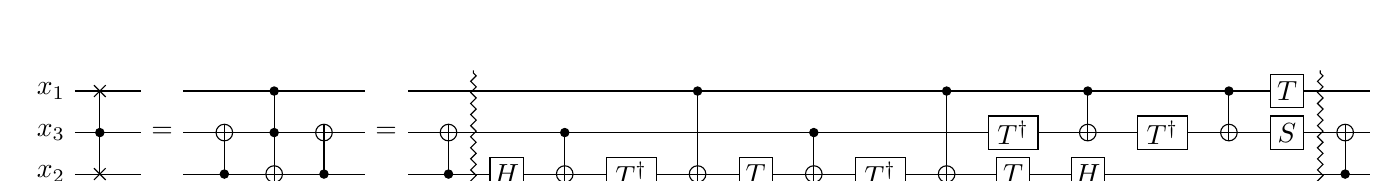
\begin{tikzpicture}[scale=1.000000,x=1pt,y=1pt]
\filldraw[color=white] (0.000000, -7.500000) rectangle (468.000000, 37.500000);
% Drawing wires
% Line 1: a3 W x_1
\draw[color=black] (0.000000,30.000000) -- (468.000000,30.000000);
\draw[color=black] (0.000000,30.000000) node[left] {$x_1$};
% Line 2: a2 W x_3
\draw[color=black] (0.000000,15.000000) -- (468.000000,15.000000);
\draw[color=black] (0.000000,15.000000) node[left] {$x_3$};
% Line 3: a1 W x_2
\draw[color=black] (0.000000,0.000000) -- (468.000000,0.000000);
\draw[color=black] (0.000000,0.000000) node[left] {$x_2$};
% Done with wires; drawing gates
% Line 4: a1 a3 SWAP a2
\draw (9.000000,30.000000) -- (9.000000,0.000000);
\begin{scope}
\draw (6.878680, -2.121320) -- (11.121320, 2.121320);
\draw (6.878680, 2.121320) -- (11.121320, -2.121320);
\end{scope}
\begin{scope}
\draw (6.878680, 27.878680) -- (11.121320, 32.121320);
\draw (6.878680, 32.121320) -- (11.121320, 27.878680);
\end{scope}
\filldraw (9.000000, 15.000000) circle(1.500000pt);
% Line 5: =
\draw[fill=white,color=white] (24.000000, -6.000000) rectangle (39.000000, 36.000000);
\draw (31.500000, 15.000000) node {$=$};
% Line 6: a1 +a2
\draw (54.000000,15.000000) -- (54.000000,0.000000);
\filldraw (54.000000, 0.000000) circle(1.500000pt);
\begin{scope}
\draw[fill=white] (54.000000, 15.000000) circle(3.000000pt);
\clip (54.000000, 15.000000) circle(3.000000pt);
\draw (51.000000, 15.000000) -- (57.000000, 15.000000);
\draw (54.000000, 12.000000) -- (54.000000, 18.000000);
\end{scope}
% Line 7: +a1 a2 a3
\draw (72.000000,30.000000) -- (72.000000,0.000000);
\begin{scope}
\draw[fill=white] (72.000000, 0.000000) circle(3.000000pt);
\clip (72.000000, 0.000000) circle(3.000000pt);
\draw (69.000000, 0.000000) -- (75.000000, 0.000000);
\draw (72.000000, -3.000000) -- (72.000000, 3.000000);
\end{scope}
\filldraw (72.000000, 15.000000) circle(1.500000pt);
\filldraw (72.000000, 30.000000) circle(1.500000pt);
% Line 8: a1 +a2
\draw (90.000000,15.000000) -- (90.000000,0.000000);
\filldraw (90.000000, 0.000000) circle(1.500000pt);
\begin{scope}
\draw[fill=white] (90.000000, 15.000000) circle(3.000000pt);
\clip (90.000000, 15.000000) circle(3.000000pt);
\draw (87.000000, 15.000000) -- (93.000000, 15.000000);
\draw (90.000000, 12.000000) -- (90.000000, 18.000000);
\end{scope}
% Line 9: =
\draw[fill=white,color=white] (105.000000, -6.000000) rectangle (120.000000, 36.000000);
\draw (112.500000, 15.000000) node {$=$};
% Line 10: a1 +a2
\draw (135.000000,15.000000) -- (135.000000,0.000000);
\filldraw (135.000000, 0.000000) circle(1.500000pt);
\begin{scope}
\draw[fill=white] (135.000000, 15.000000) circle(3.000000pt);
\clip (135.000000, 15.000000) circle(3.000000pt);
\draw (132.000000, 15.000000) -- (138.000000, 15.000000);
\draw (135.000000, 12.000000) -- (135.000000, 18.000000);
\end{scope}
% Line 11: BARRIER
\draw[decorate,decoration={zigzag,amplitude=1pt,segment length=4}] (144.000000,-7.500000) -- (144.000000,37.500000);
% Line 12: a1 H
\begin{scope}
\draw[fill=white] (156.000000, -0.000000) +(-45.000000:8.485281pt and 8.485281pt) -- +(45.000000:8.485281pt and 8.485281pt) -- +(135.000000:8.485281pt and 8.485281pt) -- +(225.000000:8.485281pt and 8.485281pt) -- cycle;
\clip (156.000000, -0.000000) +(-45.000000:8.485281pt and 8.485281pt) -- +(45.000000:8.485281pt and 8.485281pt) -- +(135.000000:8.485281pt and 8.485281pt) -- +(225.000000:8.485281pt and 8.485281pt) -- cycle;
\draw (156.000000, -0.000000) node {$H$};
\end{scope}
% Line 13: +a1 a2
\draw (177.000000,15.000000) -- (177.000000,0.000000);
\begin{scope}
\draw[fill=white] (177.000000, 0.000000) circle(3.000000pt);
\clip (177.000000, 0.000000) circle(3.000000pt);
\draw (174.000000, 0.000000) -- (180.000000, 0.000000);
\draw (177.000000, -3.000000) -- (177.000000, 3.000000);
\end{scope}
\filldraw (177.000000, 15.000000) circle(1.500000pt);
% Line 14: a1 G $T^\dagger$ width=18
\begin{scope}
\draw[fill=white] (201.000000, -0.000000) +(-45.000000:12.727922pt and 8.485281pt) -- +(45.000000:12.727922pt and 8.485281pt) -- +(135.000000:12.727922pt and 8.485281pt) -- +(225.000000:12.727922pt and 8.485281pt) -- cycle;
\clip (201.000000, -0.000000) +(-45.000000:12.727922pt and 8.485281pt) -- +(45.000000:12.727922pt and 8.485281pt) -- +(135.000000:12.727922pt and 8.485281pt) -- +(225.000000:12.727922pt and 8.485281pt) -- cycle;
\draw (201.000000, -0.000000) node {$T^\dagger$};
\end{scope}
% Line 15: +a1 a3
\draw (225.000000,30.000000) -- (225.000000,0.000000);
\begin{scope}
\draw[fill=white] (225.000000, 0.000000) circle(3.000000pt);
\clip (225.000000, 0.000000) circle(3.000000pt);
\draw (222.000000, 0.000000) -- (228.000000, 0.000000);
\draw (225.000000, -3.000000) -- (225.000000, 3.000000);
\end{scope}
\filldraw (225.000000, 30.000000) circle(1.500000pt);
% Line 16: a1 G $T$
\begin{scope}
\draw[fill=white] (246.000000, -0.000000) +(-45.000000:8.485281pt and 8.485281pt) -- +(45.000000:8.485281pt and 8.485281pt) -- +(135.000000:8.485281pt and 8.485281pt) -- +(225.000000:8.485281pt and 8.485281pt) -- cycle;
\clip (246.000000, -0.000000) +(-45.000000:8.485281pt and 8.485281pt) -- +(45.000000:8.485281pt and 8.485281pt) -- +(135.000000:8.485281pt and 8.485281pt) -- +(225.000000:8.485281pt and 8.485281pt) -- cycle;
\draw (246.000000, -0.000000) node {$T$};
\end{scope}
% Line 17: +a1 a2
\draw (267.000000,15.000000) -- (267.000000,0.000000);
\begin{scope}
\draw[fill=white] (267.000000, 0.000000) circle(3.000000pt);
\clip (267.000000, 0.000000) circle(3.000000pt);
\draw (264.000000, 0.000000) -- (270.000000, 0.000000);
\draw (267.000000, -3.000000) -- (267.000000, 3.000000);
\end{scope}
\filldraw (267.000000, 15.000000) circle(1.500000pt);
% Line 18: a1 G $T^\dagger$ width=18
\begin{scope}
\draw[fill=white] (291.000000, -0.000000) +(-45.000000:12.727922pt and 8.485281pt) -- +(45.000000:12.727922pt and 8.485281pt) -- +(135.000000:12.727922pt and 8.485281pt) -- +(225.000000:12.727922pt and 8.485281pt) -- cycle;
\clip (291.000000, -0.000000) +(-45.000000:12.727922pt and 8.485281pt) -- +(45.000000:12.727922pt and 8.485281pt) -- +(135.000000:12.727922pt and 8.485281pt) -- +(225.000000:12.727922pt and 8.485281pt) -- cycle;
\draw (291.000000, -0.000000) node {$T^\dagger$};
\end{scope}
% Line 19: +a1 a3
\draw (315.000000,30.000000) -- (315.000000,0.000000);
\begin{scope}
\draw[fill=white] (315.000000, 0.000000) circle(3.000000pt);
\clip (315.000000, 0.000000) circle(3.000000pt);
\draw (312.000000, 0.000000) -- (318.000000, 0.000000);
\draw (315.000000, -3.000000) -- (315.000000, 3.000000);
\end{scope}
\filldraw (315.000000, 30.000000) circle(1.500000pt);
% Line 20: TOUCH
% Line 21: a2 G $T^\dagger$ width=18
\begin{scope}
\draw[fill=white] (339.000000, 15.000000) +(-45.000000:12.727922pt and 8.485281pt) -- +(45.000000:12.727922pt and 8.485281pt) -- +(135.000000:12.727922pt and 8.485281pt) -- +(225.000000:12.727922pt and 8.485281pt) -- cycle;
\clip (339.000000, 15.000000) +(-45.000000:12.727922pt and 8.485281pt) -- +(45.000000:12.727922pt and 8.485281pt) -- +(135.000000:12.727922pt and 8.485281pt) -- +(225.000000:12.727922pt and 8.485281pt) -- cycle;
\draw (339.000000, 15.000000) node {$T^\dagger$};
\end{scope}
% Line 22: a1 G $T$
\begin{scope}
\draw[fill=white] (339.000000, -0.000000) +(-45.000000:8.485281pt and 8.485281pt) -- +(45.000000:8.485281pt and 8.485281pt) -- +(135.000000:8.485281pt and 8.485281pt) -- +(225.000000:8.485281pt and 8.485281pt) -- cycle;
\clip (339.000000, -0.000000) +(-45.000000:8.485281pt and 8.485281pt) -- +(45.000000:8.485281pt and 8.485281pt) -- +(135.000000:8.485281pt and 8.485281pt) -- +(225.000000:8.485281pt and 8.485281pt) -- cycle;
\draw (339.000000, -0.000000) node {$T$};
\end{scope}
% Line 23: a1 H
\begin{scope}
\draw[fill=white] (366.000000, -0.000000) +(-45.000000:8.485281pt and 8.485281pt) -- +(45.000000:8.485281pt and 8.485281pt) -- +(135.000000:8.485281pt and 8.485281pt) -- +(225.000000:8.485281pt and 8.485281pt) -- cycle;
\clip (366.000000, -0.000000) +(-45.000000:8.485281pt and 8.485281pt) -- +(45.000000:8.485281pt and 8.485281pt) -- +(135.000000:8.485281pt and 8.485281pt) -- +(225.000000:8.485281pt and 8.485281pt) -- cycle;
\draw (366.000000, -0.000000) node {$H$};
\end{scope}
% Line 24: +a2 a3
\draw (366.000000,30.000000) -- (366.000000,15.000000);
\begin{scope}
\draw[fill=white] (366.000000, 15.000000) circle(3.000000pt);
\clip (366.000000, 15.000000) circle(3.000000pt);
\draw (363.000000, 15.000000) -- (369.000000, 15.000000);
\draw (366.000000, 12.000000) -- (366.000000, 18.000000);
\end{scope}
\filldraw (366.000000, 30.000000) circle(1.500000pt);
% Line 25: a2 G $T^\dagger$ width=18
\begin{scope}
\draw[fill=white] (393.000000, 15.000000) +(-45.000000:12.727922pt and 8.485281pt) -- +(45.000000:12.727922pt and 8.485281pt) -- +(135.000000:12.727922pt and 8.485281pt) -- +(225.000000:12.727922pt and 8.485281pt) -- cycle;
\clip (393.000000, 15.000000) +(-45.000000:12.727922pt and 8.485281pt) -- +(45.000000:12.727922pt and 8.485281pt) -- +(135.000000:12.727922pt and 8.485281pt) -- +(225.000000:12.727922pt and 8.485281pt) -- cycle;
\draw (393.000000, 15.000000) node {$T^\dagger$};
\end{scope}
% Line 26: +a2 a3
\draw (417.000000,30.000000) -- (417.000000,15.000000);
\begin{scope}
\draw[fill=white] (417.000000, 15.000000) circle(3.000000pt);
\clip (417.000000, 15.000000) circle(3.000000pt);
\draw (414.000000, 15.000000) -- (420.000000, 15.000000);
\draw (417.000000, 12.000000) -- (417.000000, 18.000000);
\end{scope}
\filldraw (417.000000, 30.000000) circle(1.500000pt);
% Line 27: a3 G $T$
\begin{scope}
\draw[fill=white] (438.000000, 30.000000) +(-45.000000:8.485281pt and 8.485281pt) -- +(45.000000:8.485281pt and 8.485281pt) -- +(135.000000:8.485281pt and 8.485281pt) -- +(225.000000:8.485281pt and 8.485281pt) -- cycle;
\clip (438.000000, 30.000000) +(-45.000000:8.485281pt and 8.485281pt) -- +(45.000000:8.485281pt and 8.485281pt) -- +(135.000000:8.485281pt and 8.485281pt) -- +(225.000000:8.485281pt and 8.485281pt) -- cycle;
\draw (438.000000, 30.000000) node {$T$};
\end{scope}
% Line 28: a2 G $S$
\begin{scope}
\draw[fill=white] (438.000000, 15.000000) +(-45.000000:8.485281pt and 8.485281pt) -- +(45.000000:8.485281pt and 8.485281pt) -- +(135.000000:8.485281pt and 8.485281pt) -- +(225.000000:8.485281pt and 8.485281pt) -- cycle;
\clip (438.000000, 15.000000) +(-45.000000:8.485281pt and 8.485281pt) -- +(45.000000:8.485281pt and 8.485281pt) -- +(135.000000:8.485281pt and 8.485281pt) -- +(225.000000:8.485281pt and 8.485281pt) -- cycle;
\draw (438.000000, 15.000000) node {$S$};
\end{scope}
% Line 29: BARRIER
\draw[decorate,decoration={zigzag,amplitude=1pt,segment length=4}] (450.000000,-7.500000) -- (450.000000,37.500000);
% Line 30: a1 +a2
\draw (459.000000,15.000000) -- (459.000000,0.000000);
\filldraw (459.000000, 0.000000) circle(1.500000pt);
\begin{scope}
\draw[fill=white] (459.000000, 15.000000) circle(3.000000pt);
\clip (459.000000, 15.000000) circle(3.000000pt);
\draw (456.000000, 15.000000) -- (462.000000, 15.000000);
\draw (459.000000, 12.000000) -- (459.000000, 18.000000);
\end{scope}
% Done with gates; drawing ending labels
% Done with ending labels; drawing cut lines and comments
% Done with comments
\end{tikzpicture}
\end{center}
\vspace{-10pt}
Gates 0-3 could be combined into a single 2-qubit gate, but likely would not be in practice due to implementation difficulty.
\newpage
\Textbf{4.26} Show that the circuit:
\begin{center}
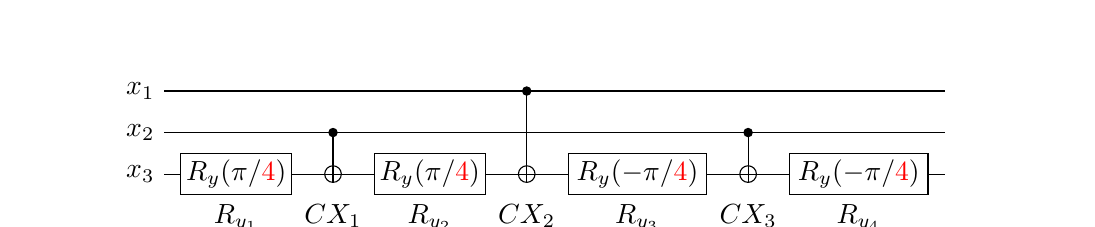
\begin{tikzpicture}[scale=1.000000,x=1pt,y=1pt]
\filldraw[color=white] (0.000000, -7.500000) rectangle (282.000000, 37.500000);
% Drawing wires
% Line 1: a3 W x_3
\draw[color=black] (0.000000,30.000000) -- (282.000000,30.000000);
\draw[color=black] (0.000000,30.000000) node[left] {$x_1$};
% Line 2: a2 W x_2
\draw[color=black] (0.000000,15.000000) -- (282.000000,15.000000);
\draw[color=black] (0.000000,15.000000) node[left] {$x_2$};
% Line 3: a1 W x_1
\draw[color=black] (0.000000,0.000000) -- (282.000000,0.000000);
\draw[color=black] (0.000000,0.000000) node[left] {$x_3$};
% Done with wires; drawing gates
% Line 4: a1 G $R_y(\pi/\textcolor{red}{4})$ width=40 height=15 %% $R_{y_1}$
\draw (26.000000, -7.500000) node[text width=144pt,below,text centered] {$R_{y_1}$};
\begin{scope}
\draw[fill=white] (26.000000, -0.000000) +(-45.000000:28.284271pt and 10.606602pt) -- +(45.000000:28.284271pt and 10.606602pt) -- +(135.000000:28.284271pt and 10.606602pt) -- +(225.000000:28.284271pt and 10.606602pt) -- cycle;
\clip (26.000000, -0.000000) +(-45.000000:28.284271pt and 10.606602pt) -- +(45.000000:28.284271pt and 10.606602pt) -- +(135.000000:28.284271pt and 10.606602pt) -- +(225.000000:28.284271pt and 10.606602pt) -- cycle;
\draw (26.000000, -0.000000) node {$R_y(\pi/\textcolor{red}{4})$};
\end{scope}
% Line 5: +a1 a2 %% $CX_1$
\draw (61.000000, -7.500000) node[text width=144pt,below,text centered] {$CX_1$};
\draw (61.000000,15.000000) -- (61.000000,0.000000);
\begin{scope}
\draw[fill=white] (61.000000, 0.000000) circle(3.000000pt);
\clip (61.000000, 0.000000) circle(3.000000pt);
\draw (58.000000, 0.000000) -- (64.000000, 0.000000);
\draw (61.000000, -3.000000) -- (61.000000, 3.000000);
\end{scope}
\filldraw (61.000000, 15.000000) circle(1.500000pt);
% Line 6: a1 G $R_y(\pi/\textcolor{red}{4})$ width=40 height=15 %% $R_{y_2}$
\draw (96.000000, -7.500000) node[text width=144pt,below,text centered] {$R_{y_2}$};
\begin{scope}
\draw[fill=white] (96.000000, -0.000000) +(-45.000000:28.284271pt and 10.606602pt) -- +(45.000000:28.284271pt and 10.606602pt) -- +(135.000000:28.284271pt and 10.606602pt) -- +(225.000000:28.284271pt and 10.606602pt) -- cycle;
\clip (96.000000, -0.000000) +(-45.000000:28.284271pt and 10.606602pt) -- +(45.000000:28.284271pt and 10.606602pt) -- +(135.000000:28.284271pt and 10.606602pt) -- +(225.000000:28.284271pt and 10.606602pt) -- cycle;
\draw (96.000000, -0.000000) node {$R_y(\pi/\textcolor{red}{4})$};
\end{scope}
% Line 7: +a1 a3 %% $CX_2$
\draw (131.000000, -7.500000) node[text width=144pt,below,text centered] {$CX_2$};
\draw (131.000000,30.000000) -- (131.000000,0.000000);
\begin{scope}
\draw[fill=white] (131.000000, 0.000000) circle(3.000000pt);
\clip (131.000000, 0.000000) circle(3.000000pt);
\draw (128.000000, 0.000000) -- (134.000000, 0.000000);
\draw (131.000000, -3.000000) -- (131.000000, 3.000000);
\end{scope}
\filldraw (131.000000, 30.000000) circle(1.500000pt);
% Line 8: a1 G $R_y(-\pi/\textcolor{red}{4})$ width=50 height=15 %% $R_{y_3}$
\draw (171.000000, -7.500000) node[text width=144pt,below,text centered] {$R_{y_3}$};
\begin{scope}
\draw[fill=white] (171.000000, -0.000000) +(-45.000000:35.355339pt and 10.606602pt) -- +(45.000000:35.355339pt and 10.606602pt) -- +(135.000000:35.355339pt and 10.606602pt) -- +(225.000000:35.355339pt and 10.606602pt) -- cycle;
\clip (171.000000, -0.000000) +(-45.000000:35.355339pt and 10.606602pt) -- +(45.000000:35.355339pt and 10.606602pt) -- +(135.000000:35.355339pt and 10.606602pt) -- +(225.000000:35.355339pt and 10.606602pt) -- cycle;
\draw (171.000000, -0.000000) node {$R_y(-\pi/\textcolor{red}{4})$};
\end{scope}
% Line 9: +a1 a2 %% $CX_3$
\draw (211.000000, -7.500000) node[text width=144pt,below,text centered] {$CX_3$};
\draw (211.000000,15.000000) -- (211.000000,0.000000);
\begin{scope}
\draw[fill=white] (211.000000, 0.000000) circle(3.000000pt);
\clip (211.000000, 0.000000) circle(3.000000pt);
\draw (208.000000, 0.000000) -- (214.000000, 0.000000);
\draw (211.000000, -3.000000) -- (211.000000, 3.000000);
\end{scope}
\filldraw (211.000000, 15.000000) circle(1.500000pt);
% Line 10: a1 G $R_y(-\pi/\textcolor{red}{4})$ width=50 height=15 %% $R_{y_4}$
\draw (251.000000, -7.500000) node[text width=144pt,below,text centered] {$R_{y_4}$};
\begin{scope}
\draw[fill=white] (251.000000, -0.000000) +(-45.000000:35.355339pt and 10.606602pt) -- +(45.000000:35.355339pt and 10.606602pt) -- +(135.000000:35.355339pt and 10.606602pt) -- +(225.000000:35.355339pt and 10.606602pt) -- cycle;
\clip (251.000000, -0.000000) +(-45.000000:35.355339pt and 10.606602pt) -- +(45.000000:35.355339pt and 10.606602pt) -- +(135.000000:35.355339pt and 10.606602pt) -- +(225.000000:35.355339pt and 10.606602pt) -- cycle;
\draw (251.000000, -0.000000) node {$R_y(-\pi/\textcolor{red}{4})$};
\end{scope}
% Done with gates; drawing ending labels
% Done with ending labels; drawing cut lines and comments
% Done with comments
\end{tikzpicture}
\end{center}
\vspace{-5pt}
differs from a Toffoli gate only by relative phases.  That is, the circuit takes $\ket{c_1, c_2, t}$ to $e^{i\theta(c_1,c_2,t)}\cdot \ket{c_1,c_2,t\oplus c_1\cdot c_2}$, where $e^{i\theta(c_1,c_2,t)}$ is some relative phase factor. Such gates can sometimes be useful in experimental implementations, where it may be much easier to implement a gate that is the same as the Toffoli up to relative phases than it is to do the Toffoli directly.
\begin{comment}
\Soln Note that $R_y(\pm\pi) = \mp iY = \begin{bmatrix} 0 & \mp1 \\ \pm 1 & 0 \end{bmatrix}$, which maps $\ket{0} \rightarrow \pm \ket{1}$ and $\ket{1}\rightarrow\mp\ket{0}$. Now, we trace the effects of the circuit on the computational basis.
\vspace{-10pt}
\begin{center}
\begin{tabular}{c|r|r|r|r|r|r|r|} 
\multicolumn{1}{c|}{$\ket{x_1x_2x_3}$} & \multicolumn{1}{c|}{$R_{y_1}$} & \multicolumn{1}{c|}{$CX_1$} & \multicolumn{1}{c|}{$R_{y_2}$ } & \multicolumn{1}{c|}{$CX_2$} & \multicolumn{1}{c|}{$R_{y_3}$ } & \multicolumn{1}{c|}{$CX_3$} & \multicolumn{1}{c|}{$R_{y_4}$} \\
\hline
$\ket{000}$ & $\ket{001}$ & $\ket{001}$ & $-\ket{000}$ & $-\ket{000}$ & $\ket{001}$ & $\ket{001}$ & $\ket{000}$ \\
\hline
$\ket{001}$ & $-\ket{000}$ & $-\ket{000}$ & $-\ket{001}$ & $-\ket{001}$ & $-\ket{000}$ & $-\ket{000}$ & $\ket{001}$ \\
\hline
$\ket{010}$ & $\ket{011}$ & $\ket{010}$ & $\ket{011}$ & $\ket{011}$ & $\ket{010}$ & $\ket{011}$ & $\ket{010}$ \\
\hline
$\ket{011}$ & $-\ket{010}$ & $-\ket{011}$ & $\ket{010}$ & $\ket{010}$ & $-\ket{011}$ & $-\ket{010}$ & $\ket{011}$ \\
\hline
$\ket{100}$ & $\ket{101}$ & $\ket{101}$ & $-\ket{100}$ & $-\ket{101}$ & $-\ket{100}$ & $-\ket{100}$ & $\ket{101}$ \\
\hline
$\ket{101}$ & $-\ket{100}$ & $-\ket{100}$ & $-\ket{101}$ & $-\ket{100}$ & $\ket{101}$ & $\ket{101}$ & $\ket{100}$ \\
\hline
$\ket{110}$ & $\ket{111}$ & $\ket{110}$ & $\ket{111}$ & $\ket{110}$ & $-\ket{111}$ & $-\ket{110}$ & $\ket{111}$ \\
\hline
$\ket{111}$ & $-\ket{110}$ & $-\ket{111}$ & $\ket{110}$  & $\ket{111}$ & $\ket{110}$ & $\ket{111}$ & $\ket{110}$ 
\end{tabular}
\end{center}
\vspace{-10pt}
That didn't work out ... it incorrectly maps $\ket{100}\rightarrow\ket{101}$ and $\ket{100}\rightarrow{101}$, effectively, this is just \CNOT$(x_1,x_3)$.
\end{comment}
\Soln Note the correction changing the rotations to $\pi/4$ instead of $\pi$.  Using rotations of $\pi$, the circuit is equivalent to a single \CNOT$(x_1, x_3)$.  Now, none of the gates alter the states of $\ket{x_1}$ or $\ket{x_2}$, so we can analyze this circuit by focusing only on it's effect on $\ket{x_3}$ while conditioning on the static state of $\ket{x_1x_2}$. First, we'll expand $R_y(\pm\pi/4)$.  Note that $\cos(\pm\pi/8) = \frac{\sqrt{2+\sqrt{2}}}{2}$, and $\sin(\pm\pi/8)=\pm\frac{\sqrt{2-\sqrt{2}}}{2}$.  Now:
$$R_y(\pm\pi/4) = \cos(\pm\pi/8)I-i\sin(\pm\pi/8)Y = \begin{bmatrix}\cos(\pm\pi/8) & -\sin(\pm\pi/8) \\ \sin(\pm\pi/8)& \cos(\pm\pi/8)\end{bmatrix} = \begin{bmatrix} \frac{\sqrt{2+\sqrt{2}}}{2} & \mp\frac{\sqrt{2-\sqrt{2}}}{2} \\ \pm\frac{\sqrt{2-\sqrt{2}}}{2} & \frac{\sqrt{2+\sqrt{2}}}{2}\end{bmatrix}.$$

When $\ket{x_1x_2}=\ket{00}$, the operations applied to $\ket{x_3}$ are $R_y(\pi/4)^2R_y(-\pi/4)^2$.  Note that $R_y(\theta)R_y(-\theta) = I$, so in this case the circuit does not change the state of $\ket{x_3}$.  When $\ket{x_1x_2} = \ket{01}$, the operations applied to $\ket{x_3}$ are $R_y(\pi/8)XR_y(\pi/8)R_y(-\pi/8)XR_y(-\pi/8)=R_y(\pi/8)X^2R_y*(-\pi/8)=R_y(\pi/8)R_y*(-\pi/8)=I$, so again, $\ket{x_3}$ is unchanged.  When $\ket{x_1x_2} = \ket{10}$, the operations are:
\begin{align*}
R_y(\pi/4)^2XR_y(-\pi/4)^2 &= R_y(\pi/2)XR_y(-\pi/2) \\
                           &= \begin{bmatrix}\frac{\sqrt{2}}{2} & - \frac{\sqrt{2}}{2} \\ \frac{\sqrt{2}}{2} &  \frac{\sqrt{2}}{2}\end{bmatrix}
                              \begin{bmatrix} 0 & 1 \\ 1 & 0 \end{bmatrix}
                              \begin{bmatrix}\frac{\sqrt{2}}{2} & \frac{\sqrt{2}}{2} \\ -\frac{\sqrt{2}}{2} &  \frac{\sqrt{2}}{2}\end{bmatrix} \\
                           &= \begin{bmatrix} -1 & 0 \\ 0 & 1\end{bmatrix}
\end{align*}
Finally, when $\ket{x_1x_2} = \ket{11}$, the operations are:
$$R_y(\pi/4)XR_y(\pi/4)XR_y(-\pi/4)XR_y(-\pi/4) = $$
$$\begin{bmatrix} \frac{\sqrt{2+\sqrt{2}}}{2} & -\frac{\sqrt{2-\sqrt{2}}}{2} \\ \frac{\sqrt{2-\sqrt{2}}}{2} & \frac{\sqrt{2+\sqrt{2}}}{2} \end{bmatrix}
\begin{bmatrix} 0 & 1 \\ 1 & 0 \end{bmatrix} 
\begin{bmatrix} \frac{\sqrt{2+\sqrt{2}}}{2} & -\frac{\sqrt{2-\sqrt{2}}}{2} \\ \frac{\sqrt{2-\sqrt{2}}}{2} & \frac{\sqrt{2+\sqrt{2}}}{2}\end{bmatrix}
\begin{bmatrix} 0 & 1 \\ 1 & 0 \end{bmatrix}
\begin{bmatrix} \frac{\sqrt{2+\sqrt{2}}}{2} & \frac{\sqrt{2-\sqrt{2}}}{2} \\ -\frac{\sqrt{2-\sqrt{2}}}{2} & \frac{\sqrt{2+\sqrt{2}}}{2}\end{bmatrix}
\begin{bmatrix} 0 & 1 \\ 1 & 0 \end{bmatrix}
\begin{bmatrix} \frac{\sqrt{2+\sqrt{2}}}{2} & \frac{\sqrt{2-\sqrt{2}}}{2} \\ -\frac{\sqrt{2-\sqrt{2}}}{2} & \frac{\sqrt{2+\sqrt{2}}}{2}\end{bmatrix} $$
$$= \begin{bmatrix} 0 & 1 \\ 1 & 0\end{bmatrix} = X$$


So, the circuit performs the transformation $$\begin{bmatrix}
1 & 0 & 0 & 0 & 0 & 0 & 0 & 0 \\
0 & 1 & 0 & 0 & 0 & 0 & 0 & 0 \\
0 & 0 & 1 & 0 & 0 & 0 & 0 & 0 \\
0 & 0 & 0 & 1 & 0 & 0 & 0 & 0 \\
0 & 0 & 0 & 0 & -1 & 0 & 0 & 0 \\
0 & 0 & 0 & 0 & 0 & 1 & 0 & 0 \\
0 & 0 & 0 & 0 & 0 & 0 & 0 & 1 \\
0 & 0 & 0 & 0 & 0 & 0 & 1 & 0 \\
\end{bmatrix}$$
This transformation matches a Toffoli gate, except that it introduces a relative phase of $\pi$ to the result of the computational basis state $\ket{100}$.

\Textbf{4.27} Using just \CNOT s and Toffoli gates, construct a quantum circuit to perform the tansformation
$$\pi = \begin{bmatrix}
1 & 0 & 0 & 0 & 0 & 0 & 0 & 0 \\
0 & 0 & 0 & 0 & 0 & 0 & 0 & 1 \\
0 & 1 & 0 & 0 & 0 & 0 & 0 & 0 \\
0 & 0 & 1 & 0 & 0 & 0 & 0 & 0 \\
0 & 0 & 0 & 1 & 0 & 0 & 0 & 0 \\
0 & 0 & 0 & 0 & 1 & 0 & 0 & 0 \\
0 & 0 & 0 & 0 & 0 & 1 & 0 & 0 \\
0 & 0 & 0 & 0 & 0 & 0 & 1 & 0 \\
\end{bmatrix}$$
This kind of partial cyclic permutation operation will be useful later, in Chapter 7.
\Soln \CNOT s and Toffoli gates permute the computational basis states as does the target transformation. But for lack of intuition, a python script was written to exhaustively search products of the permutations they represent, looking for the target transformation as the result.  A product of 5 gates was found involving 2 Toffolis and 3 \CNOT s:
\begin{center}\ \ \ \ \ \ \ \ 
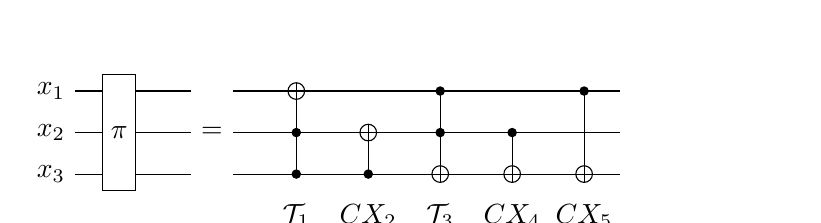
\begin{tikzpicture}[scale=1.000000,x=1pt,y=1pt]
\filldraw[color=white] (0.000000, -7.500000) rectangle (197.000000, 37.500000);
% Drawing wires
% Line 1: a1 W x_1
\draw[color=black] (0.000000,30.000000) -- (197.000000,30.000000);
\draw[color=black] (0.000000,30.000000) node[left] {$x_1$};
% Line 2: a2 W x_2
\draw[color=black] (0.000000,15.000000) -- (197.000000,15.000000);
\draw[color=black] (0.000000,15.000000) node[left] {$x_2$};
% Line 3: a3 W x_3
\draw[color=black] (0.000000,0.000000) -- (197.000000,0.000000);
\draw[color=black] (0.000000,0.000000) node[left] {$x_3$};
% Done with wires; drawing gates
% Line 4: a1 a2 a3 G $\pi$
\draw (16.000000,30.000000) -- (16.000000,0.000000);
\begin{scope}
\draw[fill=white] (16.000000, 15.000000) +(-45.000000:8.485281pt and 29.698485pt) -- +(45.000000:8.485281pt and 29.698485pt) -- +(135.000000:8.485281pt and 29.698485pt) -- +(225.000000:8.485281pt and 29.698485pt) -- cycle;
\clip (16.000000, 15.000000) +(-45.000000:8.485281pt and 29.698485pt) -- +(45.000000:8.485281pt and 29.698485pt) -- +(135.000000:8.485281pt and 29.698485pt) -- +(225.000000:8.485281pt and 29.698485pt) -- cycle;
\draw (16.000000, 15.000000) node {$\pi$};
\end{scope}
% Line 5: =
\draw[fill=white,color=white] (42.000000, -6.000000) rectangle (57.000000, 36.000000);
\draw (49.500000, 15.000000) node {$=$};
% Line 6: +a1 a2 a3 %% $\mathcal{T}_1$
\draw (80.000000, -7.500000) node[text width=144pt,below,text centered] {$\mathcal{T}_1$};
\draw (80.000000,30.000000) -- (80.000000,0.000000);
\begin{scope}
\draw[fill=white] (80.000000, 30.000000) circle(3.000000pt);
\clip (80.000000, 30.000000) circle(3.000000pt);
\draw (77.000000, 30.000000) -- (83.000000, 30.000000);
\draw (80.000000, 27.000000) -- (80.000000, 33.000000);
\end{scope}
\filldraw (80.000000, 15.000000) circle(1.500000pt);
\filldraw (80.000000, 0.000000) circle(1.500000pt);
% Line 7: +a2 a3 %% $CX_2$
\draw (106.000000, -7.500000) node[text width=144pt,below,text centered] {$CX_2$};
\draw (106.000000,15.000000) -- (106.000000,0.000000);
\begin{scope}
\draw[fill=white] (106.000000, 15.000000) circle(3.000000pt);
\clip (106.000000, 15.000000) circle(3.000000pt);
\draw (103.000000, 15.000000) -- (109.000000, 15.000000);
\draw (106.000000, 12.000000) -- (106.000000, 18.000000);
\end{scope}
\filldraw (106.000000, 0.000000) circle(1.500000pt);
% Line 8: +a3 a1 a2 %% $\mathcal{T}_3$
\draw (132.000000, -7.500000) node[text width=144pt,below,text centered] {$\mathcal{T}_3$};
\draw (132.000000,30.000000) -- (132.000000,0.000000);
\begin{scope}
\draw[fill=white] (132.000000, 0.000000) circle(3.000000pt);
\clip (132.000000, 0.000000) circle(3.000000pt);
\draw (129.000000, 0.000000) -- (135.000000, 0.000000);
\draw (132.000000, -3.000000) -- (132.000000, 3.000000);
\end{scope}
\filldraw (132.000000, 30.000000) circle(1.500000pt);
\filldraw (132.000000, 15.000000) circle(1.500000pt);
% Line 9: +a3 a2 %% $CX_4$
\draw (158.000000, -7.500000) node[text width=144pt,below,text centered] {$CX_4$};
\draw (158.000000,15.000000) -- (158.000000,0.000000);
\begin{scope}
\draw[fill=white] (158.000000, 0.000000) circle(3.000000pt);
\clip (158.000000, 0.000000) circle(3.000000pt);
\draw (155.000000, 0.000000) -- (161.000000, 0.000000);
\draw (158.000000, -3.000000) -- (158.000000, 3.000000);
\end{scope}
\filldraw (158.000000, 15.000000) circle(1.500000pt);
% Line 10: +a3 a1 %% $CX_5$
\draw (184.000000, -7.500000) node[text width=144pt,below,text centered] {$CX_5$};
\draw (184.000000,30.000000) -- (184.000000,0.000000);
\begin{scope}
\draw[fill=white] (184.000000, 0.000000) circle(3.000000pt);
\clip (184.000000, 0.000000) circle(3.000000pt);
\draw (181.000000, 0.000000) -- (187.000000, 0.000000);
\draw (184.000000, -3.000000) -- (184.000000, 3.000000);
\end{scope}
\filldraw (184.000000, 30.000000) circle(1.500000pt);
% Done with gates; drawing ending labels
% Done with ending labels; drawing cut lines and comments
% Done with comments
\end{tikzpicture}
\end{center}
\vspace{-15pt}
\begin{center}
\begin{tabular}{c|c|c|c|c|c|} 
$\ket{x_1x_2x_3}$ & $\mathcal{T}_1$ & $CX_2$ & $\mathcal{T}_3$ & $CX_4$ & $CX_5$\\
\hline
$\ket{000}$ & $\ket{000}$ & $\ket{000}$ & $\ket{000}$ & $\ket{000}$ & $\ket{000}$ \\
\hline
$\ket{001}$  & $\ket{001}$ & $\ket{011}$ & $\ket{011}$ & $\ket{010}$ & $\ket{010}$  \\
\hline
$\ket{010}$ & $\ket{010}$ & $\ket{010}$ & $\ket{010}$ & $\ket{011}$ & $\ket{011}$ \\
\hline
$\ket{011}$ & $\ket{111}$ & $\ket{101}$ & $\ket{101}$ & $\ket{101}$ & $\ket{100}$ \\
\hline
$\ket{100}$ & $\ket{100}$ & $\ket{100}$ & $\ket{100}$ & $\ket{100}$ & $\ket{101}$ \\
\hline
$\ket{101}$ & $\ket{101}$ & $\ket{111}$ & $\ket{110}$ & $\ket{111}$ & $\ket{110}$ \\
\hline
$\ket{110}$ & $\ket{110}$ & $\ket{110}$ & $\ket{111}$ & $\ket{110}$ & $\ket{111}$ \\
\hline
$\ket{111}$ & $\ket{011}$ & $\ket{001}$ & $\ket{001}$ & $\ket{001}$ & $\ket{001}$ 
\end{tabular}
\end{center}
\vspace{-10pt}
The last 3 gates effectively execute a \NOT\ on $\ket{x_3}$ if $\ket{x_1}=\ket{1}$ \textit{and/or} $\ket{x_2}=\ket{1}$.  They can be performed in any order, leading to 6 equivalent circuits realizing $\pi$.  These 6 are the only ``minimal realizations'', that is, the only circuits realizing $\pi$ using the least Toffolis and/or \CNOT s possible.  

In an effort to determine which permutations could be implemented via Toffolis and \CNOT s, the script was used to tabulate the number of permutations minimally representable as products of these gates of various lengths.  Because the usable gates are all controlled and no controlled gate alters the state $\ket{000}$, all products of such gates fix $\ket{000}$.  There are $7!=5040$ permutations of the remaining computation basis states, so there are potentially 5040 permutations of the computational basis that could be represented.  Suprisingly, at least to the second author, all of them are representable.  The following table lists counts of the minimum number of required gates:
\begin{center}
\begin{tabular}{|c|r|}
 gates & \multicolumn{1}{c|}{count} \\ \hline
0 & 1 \\ \hline
1 & 9 \\ \hline
2 & 60 \\ \hline
3 & 261 \\ \hline
4 & 845 \\ \hline
5 & 1784 \\ \hline
6 & 1688 \\ \hline
7 & 386 \\ \hline
8 & 6
\end{tabular}
\end{center}
\vspace{-5pt} The unique permutation representable as a product of 0 \CNOT s and/or Toffolis is, of course, the identity.  The 9 representable as products of single gates are the gates themselves.  There are $9^2=81$ possible products of two gates, 9 of which consist of a repeated gate and so produce the identity.  There are 3 types of symmetries that cause 12 of the 81 pairs to produce the same non-identity result, so the 81 pairs ultimately only produce 60 dinstinct permutations as products of 2 \CNOT s and/or Toffolis.  The symmetries are depicted below.
\begin{center}
\ \ \ \ 
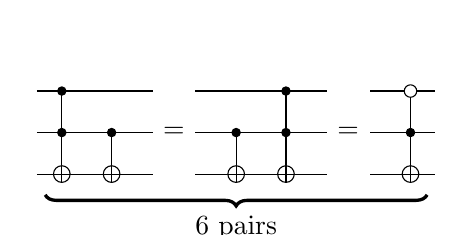
\begin{tikzpicture}[scale=1.000000,x=1pt,y=1pt]
\filldraw[color=white] (0.000000, -7.500000) rectangle (144.000000, 37.500000);
% Drawing wires
% Line 1: a1 W
\draw[color=black] (0.000000,30.000000) -- (144.000000,30.000000);
% Line 2: a2 W
\draw[color=black] (0.000000,15.000000) -- (144.000000,15.000000);
% Line 3: a3 W
\draw[color=black] (0.000000,0.000000) -- (144.000000,0.000000);
% Done with wires; drawing gates
% Line 4: a1 a2 +a3
\draw (9.000000,30.000000) -- (9.000000,0.000000);
\filldraw (9.000000, 30.000000) circle(1.500000pt);
\filldraw (9.000000, 15.000000) circle(1.500000pt);
\begin{scope}
\draw[fill=white] (9.000000, 0.000000) circle(3.000000pt);
\clip (9.000000, 0.000000) circle(3.000000pt);
\draw (6.000000, 0.000000) -- (12.000000, 0.000000);
\draw (9.000000, -3.000000) -- (9.000000, 3.000000);
\end{scope}
% Line 5: a2 +a3
\draw (27.000000,15.000000) -- (27.000000,0.000000);
\filldraw (27.000000, 15.000000) circle(1.500000pt);
\begin{scope}
\draw[fill=white] (27.000000, 0.000000) circle(3.000000pt);
\clip (27.000000, 0.000000) circle(3.000000pt);
\draw (24.000000, 0.000000) -- (30.000000, 0.000000);
\draw (27.000000, -3.000000) -- (27.000000, 3.000000);
\end{scope}
% Line 6: =
\draw[fill=white,color=white] (42.000000, -6.000000) rectangle (57.000000, 36.000000);
\draw (49.500000, 15.000000) node {$=$};
% Line 7: a2 +a3
\draw (72.000000,15.000000) -- (72.000000,0.000000);
\filldraw (72.000000, 15.000000) circle(1.500000pt);
\begin{scope}
\draw[fill=white] (72.000000, 0.000000) circle(3.000000pt);
\clip (72.000000, 0.000000) circle(3.000000pt);
\draw (69.000000, 0.000000) -- (75.000000, 0.000000);
\draw (72.000000, -3.000000) -- (72.000000, 3.000000);
\end{scope}
% Line 8: a1 a2 +a3
\draw (90.000000,30.000000) -- (90.000000,0.000000);
\filldraw (90.000000, 30.000000) circle(1.500000pt);
\filldraw (90.000000, 15.000000) circle(1.500000pt);
\begin{scope}
\draw[fill=white] (90.000000, 0.000000) circle(3.000000pt);
\clip (90.000000, 0.000000) circle(3.000000pt);
\draw (87.000000, 0.000000) -- (93.000000, 0.000000);
\draw (90.000000, -3.000000) -- (90.000000, 3.000000);
\end{scope}
% Line 9: =
\draw[fill=white,color=white] (105.000000, -6.000000) rectangle (120.000000, 36.000000);
\draw (112.500000, 15.000000) node {$=$};
% Line 10: -a1 a2 +a3
\draw (135.000000,30.000000) -- (135.000000,0.000000);
\draw[fill=white] (135.000000, 30.000000) circle(2.250000pt);
\filldraw (135.000000, 15.000000) circle(1.500000pt);
\begin{scope}
\draw[fill=white] (135.000000, 0.000000) circle(3.000000pt);
\clip (135.000000, 0.000000) circle(3.000000pt);
\draw (132.000000, 0.000000) -- (138.000000, 0.000000);
\draw (135.000000, -3.000000) -- (135.000000, 3.000000);
\end{scope}
% Done with gates; drawing ending labels
% Done with ending labels; drawing cut lines and comments
% Line 11: @ 7 %% 6 pairs
\draw[decorate,decoration={brace,mirror,amplitude = 4.000000pt},very thick] (3.000000,-7.500000) -- (141.000000,-7.500000);
\draw (72.000000, -11.500000) node[text width=144pt,below,text centered] {6 pairs};
% Done with comments
\end{tikzpicture}
\ \ \ \ \ \ 
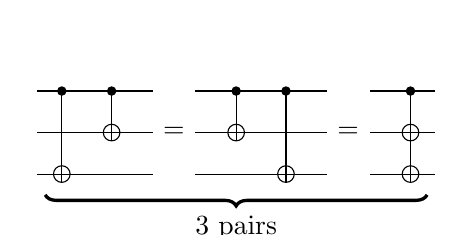
\begin{tikzpicture}[scale=1.000000,x=1pt,y=1pt]
\filldraw[color=white] (0.000000, -7.500000) rectangle (144.000000, 37.500000);
% Drawing wires
% Line 1: a1 W
\draw[color=black] (0.000000,30.000000) -- (144.000000,30.000000);
% Line 2: a2 W
\draw[color=black] (0.000000,15.000000) -- (144.000000,15.000000);
% Line 3: a3 W
\draw[color=black] (0.000000,0.000000) -- (144.000000,0.000000);
% Done with wires; drawing gates
% Line 4: a1 +a3
\draw (9.000000,30.000000) -- (9.000000,0.000000);
\filldraw (9.000000, 30.000000) circle(1.500000pt);
\begin{scope}
\draw[fill=white] (9.000000, 0.000000) circle(3.000000pt);
\clip (9.000000, 0.000000) circle(3.000000pt);
\draw (6.000000, 0.000000) -- (12.000000, 0.000000);
\draw (9.000000, -3.000000) -- (9.000000, 3.000000);
\end{scope}
% Line 5: a1 +a2
\draw (27.000000,30.000000) -- (27.000000,15.000000);
\filldraw (27.000000, 30.000000) circle(1.500000pt);
\begin{scope}
\draw[fill=white] (27.000000, 15.000000) circle(3.000000pt);
\clip (27.000000, 15.000000) circle(3.000000pt);
\draw (24.000000, 15.000000) -- (30.000000, 15.000000);
\draw (27.000000, 12.000000) -- (27.000000, 18.000000);
\end{scope}
% Line 6: =
\draw[fill=white,color=white] (42.000000, -6.000000) rectangle (57.000000, 36.000000);
\draw (49.500000, 15.000000) node {$=$};
% Line 7: a1 +a2
\draw (72.000000,30.000000) -- (72.000000,15.000000);
\filldraw (72.000000, 30.000000) circle(1.500000pt);
\begin{scope}
\draw[fill=white] (72.000000, 15.000000) circle(3.000000pt);
\clip (72.000000, 15.000000) circle(3.000000pt);
\draw (69.000000, 15.000000) -- (75.000000, 15.000000);
\draw (72.000000, 12.000000) -- (72.000000, 18.000000);
\end{scope}
% Line 8: a1 +a3
\draw (90.000000,30.000000) -- (90.000000,0.000000);
\filldraw (90.000000, 30.000000) circle(1.500000pt);
\begin{scope}
\draw[fill=white] (90.000000, 0.000000) circle(3.000000pt);
\clip (90.000000, 0.000000) circle(3.000000pt);
\draw (87.000000, 0.000000) -- (93.000000, 0.000000);
\draw (90.000000, -3.000000) -- (90.000000, 3.000000);
\end{scope}
% Line 9: =
\draw[fill=white,color=white] (105.000000, -6.000000) rectangle (120.000000, 36.000000);
\draw (112.500000, 15.000000) node {$=$};
% Line 10: a1 +a2 +a3
\draw (135.000000,30.000000) -- (135.000000,0.000000);
\filldraw (135.000000, 30.000000) circle(1.500000pt);
\begin{scope}
\draw[fill=white] (135.000000, 15.000000) circle(3.000000pt);
\clip (135.000000, 15.000000) circle(3.000000pt);
\draw (132.000000, 15.000000) -- (138.000000, 15.000000);
\draw (135.000000, 12.000000) -- (135.000000, 18.000000);
\end{scope}
\begin{scope}
\draw[fill=white] (135.000000, 0.000000) circle(3.000000pt);
\clip (135.000000, 0.000000) circle(3.000000pt);
\draw (132.000000, 0.000000) -- (138.000000, 0.000000);
\draw (135.000000, -3.000000) -- (135.000000, 3.000000);
\end{scope}
% Done with gates; drawing ending labels
% Done with ending labels; drawing cut lines and comments
% Line 11: @ 7 %% 3 pairs
\draw[decorate,decoration={brace,mirror,amplitude = 4.000000pt},very thick] (3.000000,-7.500000) -- (141.000000,-7.500000);
\draw (72.000000, -11.500000) node[text width=144pt,below,text centered] {3 pairs};
% Done with comments
\end{tikzpicture}
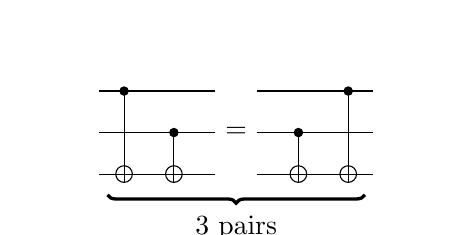
\begin{tikzpicture}[scale=1.000000,x=1pt,y=1pt]
\filldraw[color=white] (0.000000, -7.500000) rectangle (99.000000, 37.500000);
% Drawing wires
% Line 1: a1 W
\draw[color=black] (0.000000,30.000000) -- (99.000000,30.000000);
% Line 2: a2 W
\draw[color=black] (0.000000,15.000000) -- (99.000000,15.000000);
% Line 3: a3 W
\draw[color=black] (0.000000,0.000000) -- (99.000000,0.000000);
% Done with wires; drawing gates
% Line 4: a1 +a3
\draw (9.000000,30.000000) -- (9.000000,0.000000);
\filldraw (9.000000, 30.000000) circle(1.500000pt);
\begin{scope}
\draw[fill=white] (9.000000, 0.000000) circle(3.000000pt);
\clip (9.000000, 0.000000) circle(3.000000pt);
\draw (6.000000, 0.000000) -- (12.000000, 0.000000);
\draw (9.000000, -3.000000) -- (9.000000, 3.000000);
\end{scope}
% Line 5: a2 +a3
\draw (27.000000,15.000000) -- (27.000000,0.000000);
\filldraw (27.000000, 15.000000) circle(1.500000pt);
\begin{scope}
\draw[fill=white] (27.000000, 0.000000) circle(3.000000pt);
\clip (27.000000, 0.000000) circle(3.000000pt);
\draw (24.000000, 0.000000) -- (30.000000, 0.000000);
\draw (27.000000, -3.000000) -- (27.000000, 3.000000);
\end{scope}
% Line 6: =
\draw[fill=white,color=white] (42.000000, -6.000000) rectangle (57.000000, 36.000000);
\draw (49.500000, 15.000000) node {$=$};
% Line 7: a2 +a3
\draw (72.000000,15.000000) -- (72.000000,0.000000);
\filldraw (72.000000, 15.000000) circle(1.500000pt);
\begin{scope}
\draw[fill=white] (72.000000, 0.000000) circle(3.000000pt);
\clip (72.000000, 0.000000) circle(3.000000pt);
\draw (69.000000, 0.000000) -- (75.000000, 0.000000);
\draw (72.000000, -3.000000) -- (72.000000, 3.000000);
\end{scope}
% Line 8: a1 +a3
\draw (90.000000,30.000000) -- (90.000000,0.000000);
\filldraw (90.000000, 30.000000) circle(1.500000pt);
\begin{scope}
\draw[fill=white] (90.000000, 0.000000) circle(3.000000pt);
\clip (90.000000, 0.000000) circle(3.000000pt);
\draw (87.000000, 0.000000) -- (93.000000, 0.000000);
\draw (90.000000, -3.000000) -- (90.000000, 3.000000);
\end{scope}
% Done with gates; drawing ending labels
% Done with ending labels; drawing cut lines and comments
% Line 9: @ %% 3 pairs
\draw[decorate,decoration={brace,mirror,amplitude = 3.000000pt},very thick] (3.000000,-7.500000) -- (96.000000,-7.500000);
\draw (49.500000, -11.500000) node[text width=144pt,below,text centered] {3 pairs};
% Done with comments
\end{tikzpicture}
\end{center}
\vspace{-10pt}
\Textbf{4.28} For $U=V^2$ with $V$ unitary, construct a $C^5(U)$ gate analogous to that in Figure 4.10, but using no work qubits.  You may use controlled-$V$ and controlled-$V^\dagger$ gates.
\Soln NOTE: this task is only feasible if ``controlled-$V$ and controlled-$V^\dagger$ gates'' is interpreted to mean $C(V)$, $C(V^\dagger)$, \underline{and} $C^4(V)$, along with $C^4(X)$ gates. The $C^4(V)$ gate will implicitly require the existence of a unitary gate $W$ such that $W^2=V$ and the use of $C(W)$, $C(W^\dagger)$, $C^3(W)$ and $C^3(X)$ gates, which in turn require the existence of a unitary gate $P$ such that $P^2=W$ and the use of $C(P)$, $C(P^\dagger)$, $C^2(P)$ and $C^2(X)$ (Toffoli) gates.  Finally, the $C^2(P)$ gate requires the existence of unitary $Q$ such that $Q^2=P$ and the use of controlled-$Q$, controlled-$Q^\dagger$ along with $C(X)$ gates.  We'll construct $C^n(X)$ gates from Toffolis and 2-qubit gate in Exercise 4.29.  In Exercise 4.24 we constructed Toffoli gates from 2-qubit gates, but still, in order to execute a $C^n(U)$ using \underline{only} 1- and 2-qubit gates, we'd need a 1-qubit gate performing a unitary operator whose $2^n$-th power is $U$.  This gate may be guaranteed to exist theoretically, possibly under suitable hypotheses, but is almost certainly extremely difficult to implement physically.  So, a construction of such a circuit is of questionable value.  Instead, we offer a circuit using $C(V), C(V^\dagger)$ and $C^4(V)$.  The circuits using $C^3(W)$, $C^2(P)$, and $C(Q)$ can be constructed recursively in turn.  For a relatively rigorous mathematical proof of the infeasibility of the exercise without the use of $C^4(V)$-gates, see Wilfred Lee's answer to this cs.stackexchange question \href{_}\url{https://cs.stackexchange.com/questions/80538/is-it-possible-to-construct-a-c5u-with-v2-u-and-no-work-qubits-nielsen-ch}
\begin{center}
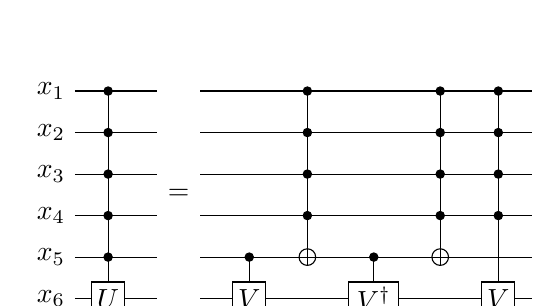
\begin{tikzpicture}[scale=1.000000,x=1pt,y=1pt]
\filldraw[color=white] (0.000000, -7.500000) rectangle (165.000000, 82.500000);
% Drawing wires
% Line 1: a1 W x_1
\draw[color=black] (0.000000,75.000000) -- (165.000000,75.000000);
\draw[color=black] (0.000000,75.000000) node[left] {$x_1$};
% Line 2: a2 W x_2
\draw[color=black] (0.000000,60.000000) -- (165.000000,60.000000);
\draw[color=black] (0.000000,60.000000) node[left] {$x_2$};
% Line 3: a3 W x_3
\draw[color=black] (0.000000,45.000000) -- (165.000000,45.000000);
\draw[color=black] (0.000000,45.000000) node[left] {$x_3$};
% Line 4: a4 W x_4
\draw[color=black] (0.000000,30.000000) -- (165.000000,30.000000);
\draw[color=black] (0.000000,30.000000) node[left] {$x_4$};
% Line 5: a5 W x_5
\draw[color=black] (0.000000,15.000000) -- (165.000000,15.000000);
\draw[color=black] (0.000000,15.000000) node[left] {$x_5$};
% Line 6: a6 W x_6
\draw[color=black] (0.000000,0.000000) -- (165.000000,0.000000);
\draw[color=black] (0.000000,0.000000) node[left] {$x_6$};
% Done with wires; drawing gates
% Line 7: a6 G $U$ a1 a2 a3 a4 a5
\draw (12.000000,75.000000) -- (12.000000,0.000000);
\begin{scope}
\draw[fill=white] (12.000000, -0.000000) +(-45.000000:8.485281pt and 8.485281pt) -- +(45.000000:8.485281pt and 8.485281pt) -- +(135.000000:8.485281pt and 8.485281pt) -- +(225.000000:8.485281pt and 8.485281pt) -- cycle;
\clip (12.000000, -0.000000) +(-45.000000:8.485281pt and 8.485281pt) -- +(45.000000:8.485281pt and 8.485281pt) -- +(135.000000:8.485281pt and 8.485281pt) -- +(225.000000:8.485281pt and 8.485281pt) -- cycle;
\draw (12.000000, -0.000000) node {$U$};
\end{scope}
\filldraw (12.000000, 75.000000) circle(1.500000pt);
\filldraw (12.000000, 60.000000) circle(1.500000pt);
\filldraw (12.000000, 45.000000) circle(1.500000pt);
\filldraw (12.000000, 30.000000) circle(1.500000pt);
\filldraw (12.000000, 15.000000) circle(1.500000pt);
% Line 8: =
\draw[fill=white,color=white] (30.000000, -6.000000) rectangle (45.000000, 81.000000);
\draw (37.500000, 37.500000) node {$=$};
% Line 9: a6 G $V$ a5
\draw (63.000000,15.000000) -- (63.000000,0.000000);
\begin{scope}
\draw[fill=white] (63.000000, -0.000000) +(-45.000000:8.485281pt and 8.485281pt) -- +(45.000000:8.485281pt and 8.485281pt) -- +(135.000000:8.485281pt and 8.485281pt) -- +(225.000000:8.485281pt and 8.485281pt) -- cycle;
\clip (63.000000, -0.000000) +(-45.000000:8.485281pt and 8.485281pt) -- +(45.000000:8.485281pt and 8.485281pt) -- +(135.000000:8.485281pt and 8.485281pt) -- +(225.000000:8.485281pt and 8.485281pt) -- cycle;
\draw (63.000000, -0.000000) node {$V$};
\end{scope}
\filldraw (63.000000, 15.000000) circle(1.500000pt);
% Line 10: a1 a2 a3 a4 +a5
\draw (84.000000,75.000000) -- (84.000000,15.000000);
\filldraw (84.000000, 75.000000) circle(1.500000pt);
\filldraw (84.000000, 60.000000) circle(1.500000pt);
\filldraw (84.000000, 45.000000) circle(1.500000pt);
\filldraw (84.000000, 30.000000) circle(1.500000pt);
\begin{scope}
\draw[fill=white] (84.000000, 15.000000) circle(3.000000pt);
\clip (84.000000, 15.000000) circle(3.000000pt);
\draw (81.000000, 15.000000) -- (87.000000, 15.000000);
\draw (84.000000, 12.000000) -- (84.000000, 18.000000);
\end{scope}
% Line 11: a6 G $V^\dagger$  a5 width=18
\draw (108.000000,15.000000) -- (108.000000,0.000000);
\begin{scope}
\draw[fill=white] (108.000000, -0.000000) +(-45.000000:12.727922pt and 8.485281pt) -- +(45.000000:12.727922pt and 8.485281pt) -- +(135.000000:12.727922pt and 8.485281pt) -- +(225.000000:12.727922pt and 8.485281pt) -- cycle;
\clip (108.000000, -0.000000) +(-45.000000:12.727922pt and 8.485281pt) -- +(45.000000:12.727922pt and 8.485281pt) -- +(135.000000:12.727922pt and 8.485281pt) -- +(225.000000:12.727922pt and 8.485281pt) -- cycle;
\draw (108.000000, -0.000000) node {$V^\dagger$};
\end{scope}
\filldraw (108.000000, 15.000000) circle(1.500000pt);
% Line 12: a1 a2 a3 a4 +a5
\draw (132.000000,75.000000) -- (132.000000,15.000000);
\filldraw (132.000000, 75.000000) circle(1.500000pt);
\filldraw (132.000000, 60.000000) circle(1.500000pt);
\filldraw (132.000000, 45.000000) circle(1.500000pt);
\filldraw (132.000000, 30.000000) circle(1.500000pt);
\begin{scope}
\draw[fill=white] (132.000000, 15.000000) circle(3.000000pt);
\clip (132.000000, 15.000000) circle(3.000000pt);
\draw (129.000000, 15.000000) -- (135.000000, 15.000000);
\draw (132.000000, 12.000000) -- (132.000000, 18.000000);
\end{scope}
% Line 13: a6 G $V$ a1 a2 a3 a4
\draw (153.000000,75.000000) -- (153.000000,0.000000);
\begin{scope}
\draw[fill=white] (153.000000, -0.000000) +(-45.000000:8.485281pt and 8.485281pt) -- +(45.000000:8.485281pt and 8.485281pt) -- +(135.000000:8.485281pt and 8.485281pt) -- +(225.000000:8.485281pt and 8.485281pt) -- cycle;
\clip (153.000000, -0.000000) +(-45.000000:8.485281pt and 8.485281pt) -- +(45.000000:8.485281pt and 8.485281pt) -- +(135.000000:8.485281pt and 8.485281pt) -- +(225.000000:8.485281pt and 8.485281pt) -- cycle;
\draw (153.000000, -0.000000) node {$V$};
\end{scope}
\filldraw (153.000000, 75.000000) circle(1.500000pt);
\filldraw (153.000000, 60.000000) circle(1.500000pt);
\filldraw (153.000000, 45.000000) circle(1.500000pt);
\filldraw (153.000000, 30.000000) circle(1.500000pt);
% Done with gates; drawing ending labels
% Done with ending labels; drawing cut lines and comments
% Done with comments
\end{tikzpicture}
\end{center}
\vspace{-10pt}
The verification of this circuit is identical to that of the circuit in figure 8 in Exercise 4.21, where instead of checking each computational basis state of $\ket{x_1}\ket{x_2}$, we check the states of $\ket{x_1x_2x_3x_4}\ket{x_5}$, where the possible states of $\ket{x_5}$ are the usual $\ket{0}$ and $\ket{1}$, but the states of $\ket{x_1x_2x_3x_4}$ are $\ket{1111}$ and $\neg\ket{1111}$, \textit{i.e.} anything other than $\ket{1111}$.

\Textbf{4.29} Find a circuit containing $O(n^2)$ Toffoli, \CNOT\ and single qubit gates which implements a $C^n(X)$ gate (for $n>3$), using no work qubits.
\Soln This exercise is also impossible as specified and interpreted naturally.
\begin{comment}  A succinct proof is offered by Craig Gidney in various placed, in particular here: \href{_}\url{https://algassert.com/circuits/2015/06/05/Constructing-Large-Controlled-Nots.html}.  We summarize
\end{comment}
\Textbf{4.30}
\Textbf{4.31} \textbf{(More circuit identities)}  Let subscripts denote which qubit an operator acts on, and let C be a \CNOT\ with qubit 1 the control and qubit 2 the target qubit.  Prove the following identities:
\begin{center}
\begin{tikzpicture}[scale=1.000000,x=1pt,y=1pt]
\filldraw[color=white] (0.000000, -7.500000) rectangle (99.000000, 22.500000);
% Drawing wires
% Line 1: a1 W x_1
\draw[color=black] (0.000000,15.000000) -- (99.000000,15.000000);
\draw[color=black] (0.000000,15.000000) node[left] {$x_1$};
% Line 2: a2 W x_2
\draw[color=black] (0.000000,0.000000) -- (99.000000,0.000000);
\draw[color=black] (0.000000,0.000000) node[left] {$x_2$};
% Done with wires; drawing gates
% Line 3: a1 +a2 % $C$ % 1
\draw (9.000000, 22.500000) node[text width=144pt,above,text centered] {$C$};
\draw (9.000000, -7.500000) node[text width=144pt,below,text centered] {1};
\draw (9.000000,15.000000) -- (9.000000,0.000000);
\filldraw (9.000000, 15.000000) circle(1.500000pt);
\begin{scope}
\draw[fill=white] (9.000000, 0.000000) circle(3.000000pt);
\clip (9.000000, 0.000000) circle(3.000000pt);
\draw (6.000000, 0.000000) -- (12.000000, 0.000000);
\draw (9.000000, -3.000000) -- (9.000000, 3.000000);
\end{scope}
% Line 4: +a1 % $X_1$ % 2
\draw (27.000000, 22.500000) node[text width=144pt,above,text centered] {$X_1$};
\draw (27.000000, -7.500000) node[text width=144pt,below,text centered] {2};
\begin{scope}
\draw[fill=white] (27.000000, 15.000000) circle(3.000000pt);
\clip (27.000000, 15.000000) circle(3.000000pt);
\draw (24.000000, 15.000000) -- (30.000000, 15.000000);
\draw (27.000000, 12.000000) -- (27.000000, 18.000000);
\end{scope}
% Line 5: a1 +a2 % $C$ % 3
\draw (45.000000, 22.500000) node[text width=144pt,above,text centered] {$C$};
\draw (45.000000, -7.500000) node[text width=144pt,below,text centered] {3};
\draw (45.000000,15.000000) -- (45.000000,0.000000);
\filldraw (45.000000, 15.000000) circle(1.500000pt);
\begin{scope}
\draw[fill=white] (45.000000, 0.000000) circle(3.000000pt);
\clip (45.000000, 0.000000) circle(3.000000pt);
\draw (42.000000, 0.000000) -- (48.000000, 0.000000);
\draw (45.000000, -3.000000) -- (45.000000, 3.000000);
\end{scope}
% Line 6: = % =
\draw (67.500000, 22.500000) node[text width=144pt,above,text centered] {=};
\draw[fill=white,color=white] (60.000000, -6.000000) rectangle (75.000000, 21.000000);
\draw (67.500000, 7.500000) node {$=$};
% Line 7: +a1
\begin{scope}
\draw[fill=white] (90.000000, 15.000000) circle(3.000000pt);
\clip (90.000000, 15.000000) circle(3.000000pt);
\draw (87.000000, 15.000000) -- (93.000000, 15.000000);
\draw (90.000000, 12.000000) -- (90.000000, 18.000000);
\end{scope}
% Line 8: +a2  %$X_1X_2$ %  4
\draw (90.000000, 22.500000) node[text width=144pt,above,text centered] {$X_1X_2$};
\draw (90.000000, -7.500000) node[text width=144pt,below,text centered] {4};
\begin{scope}
\draw[fill=white] (90.000000, 0.000000) circle(3.000000pt);
\clip (90.000000, 0.000000) circle(3.000000pt);
\draw (87.000000, 0.000000) -- (93.000000, 0.000000);
\draw (90.000000, -3.000000) -- (90.000000, 3.000000);
\end{scope}
% Done with gates; drawing ending labels
% Done with ending labels; drawing cut lines and comments
% Done with comments
\end{tikzpicture}

\begin{tabular}{c|r|r|r||r} 
$\ket{x_1x_2}$ & \multicolumn{1}{c|}{1} & \multicolumn{1}{c|}{2} & \multicolumn{1}{c||}{3} & \multicolumn{1}{c}{4} \\
\hline
$\ket{00}$ & $\ket{00}$ & $\ket{10}$ & $\ket{11}$ & $\ket{11}$ \\
\hline
$\ket{01}$ & $\ket{01}$ & $\ket{11}$ & $\ket{10}$ & $\ket{10}$ \\
\hline
$\ket{10}$ & $\ket{11}$ & $\ket{01}$ & $\ket{01}$ & $\ket{01}$ \\
\hline
$\ket{11}$ & $\ket{10}$ & $\ket{00}$ & $\ket{00}$ & $\ket{00}$ \\
\end{tabular}
\end{center}
\noindent\rule{\textwidth}{1pt}
\begin{center}
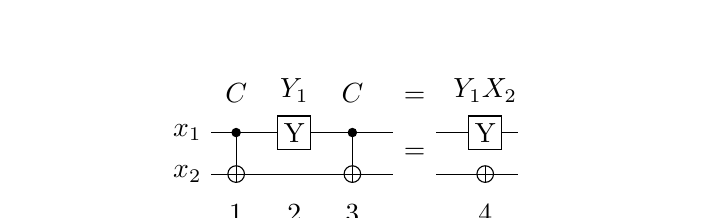
\begin{tikzpicture}[scale=1.000000,x=1pt,y=1pt]
\filldraw[color=white] (0.000000, -7.500000) rectangle (111.000000, 22.500000);
% Drawing wires
% Line 1: a1 W x_1
\draw[color=black] (0.000000,15.000000) -- (111.000000,15.000000);
\draw[color=black] (0.000000,15.000000) node[left] {$x_1$};
% Line 2: a2 W x_2
\draw[color=black] (0.000000,0.000000) -- (111.000000,0.000000);
\draw[color=black] (0.000000,0.000000) node[left] {$x_2$};
% Done with wires; drawing gates
% Line 3: a1 +a2 % $C$ % 1
\draw (9.000000, 22.500000) node[text width=144pt,above,text centered] {$C$};
\draw (9.000000, -7.500000) node[text width=144pt,below,text centered] {1};
\draw (9.000000,15.000000) -- (9.000000,0.000000);
\filldraw (9.000000, 15.000000) circle(1.500000pt);
\begin{scope}
\draw[fill=white] (9.000000, 0.000000) circle(3.000000pt);
\clip (9.000000, 0.000000) circle(3.000000pt);
\draw (6.000000, 0.000000) -- (12.000000, 0.000000);
\draw (9.000000, -3.000000) -- (9.000000, 3.000000);
\end{scope}
% Line 4: a1 G Y % $Y_1$ % 2
\draw (30.000000, 22.500000) node[text width=144pt,above,text centered] {$Y_1$};
\draw (30.000000, -7.500000) node[text width=144pt,below,text centered] {2};
\begin{scope}
\draw[fill=white] (30.000000, 15.000000) +(-45.000000:8.485281pt and 8.485281pt) -- +(45.000000:8.485281pt and 8.485281pt) -- +(135.000000:8.485281pt and 8.485281pt) -- +(225.000000:8.485281pt and 8.485281pt) -- cycle;
\clip (30.000000, 15.000000) +(-45.000000:8.485281pt and 8.485281pt) -- +(45.000000:8.485281pt and 8.485281pt) -- +(135.000000:8.485281pt and 8.485281pt) -- +(225.000000:8.485281pt and 8.485281pt) -- cycle;
\draw (30.000000, 15.000000) node {Y};
\end{scope}
% Line 5: a1 +a2 % $C$ % 3
\draw (51.000000, 22.500000) node[text width=144pt,above,text centered] {$C$};
\draw (51.000000, -7.500000) node[text width=144pt,below,text centered] {3};
\draw (51.000000,15.000000) -- (51.000000,0.000000);
\filldraw (51.000000, 15.000000) circle(1.500000pt);
\begin{scope}
\draw[fill=white] (51.000000, 0.000000) circle(3.000000pt);
\clip (51.000000, 0.000000) circle(3.000000pt);
\draw (48.000000, 0.000000) -- (54.000000, 0.000000);
\draw (51.000000, -3.000000) -- (51.000000, 3.000000);
\end{scope}
% Line 6: = % =
\draw (73.500000, 22.500000) node[text width=144pt,above,text centered] {=};
\draw[fill=white,color=white] (66.000000, -6.000000) rectangle (81.000000, 21.000000);
\draw (73.500000, 7.500000) node {$=$};
% Line 7: a1 G Y
\begin{scope}
\draw[fill=white] (99.000000, 15.000000) +(-45.000000:8.485281pt and 8.485281pt) -- +(45.000000:8.485281pt and 8.485281pt) -- +(135.000000:8.485281pt and 8.485281pt) -- +(225.000000:8.485281pt and 8.485281pt) -- cycle;
\clip (99.000000, 15.000000) +(-45.000000:8.485281pt and 8.485281pt) -- +(45.000000:8.485281pt and 8.485281pt) -- +(135.000000:8.485281pt and 8.485281pt) -- +(225.000000:8.485281pt and 8.485281pt) -- cycle;
\draw (99.000000, 15.000000) node {Y};
\end{scope}
% Line 8: +a2  %$Y_1X_2$ %  4
\draw (99.000000, 22.500000) node[text width=144pt,above,text centered] {$Y_1X_2$};
\draw (99.000000, -7.500000) node[text width=144pt,below,text centered] {4};
\begin{scope}
\draw[fill=white] (99.000000, 0.000000) circle(3.000000pt);
\clip (99.000000, 0.000000) circle(3.000000pt);
\draw (96.000000, 0.000000) -- (102.000000, 0.000000);
\draw (99.000000, -3.000000) -- (99.000000, 3.000000);
\end{scope}
% Done with gates; drawing ending labels
% Done with ending labels; drawing cut lines and comments
% Done with comments
\end{tikzpicture}

\begin{tabular}{c|r|r|r||r} 
$\ket{x_1x_2}$ & \multicolumn{1}{c|}{1} & \multicolumn{1}{c|}{2} & \multicolumn{1}{c||}{3} & \multicolumn{1}{c}{4} \\
\hline
$\ket{00}$ & $\ket{00}$ & $i\ket{10}$ & $i\ket{11}$ & $i\ket{11}$ \\
\hline
$\ket{01}$ & $\ket{01}$ & $i\ket{11}$ & $i\ket{10}$ & $i\ket{10}$ \\
\hline
$\ket{10}$ & $\ket{11}$ & $-i\ket{01}$ & $-i\ket{01}$ & $-i\ket{01}$ \\
\hline
$\ket{11}$ & $\ket{10}$ & $-i\ket{00}$ & $-i\ket{00}$ & $-i\ket{00}$ \\
\end{tabular}
\end{center}
\noindent\rule{\textwidth}{1pt}
\begin{center}
\begin{tikzpicture}[scale=1.000000,x=1pt,y=1pt]
\filldraw[color=white] (0.000000, -7.500000) rectangle (111.000000, 22.500000);
% Drawing wires
% Line 1: a1 W x_1
\draw[color=black] (0.000000,15.000000) -- (111.000000,15.000000);
\draw[color=black] (0.000000,15.000000) node[left] {$x_1$};
% Line 2: a2 W x_2
\draw[color=black] (0.000000,0.000000) -- (111.000000,0.000000);
\draw[color=black] (0.000000,0.000000) node[left] {$x_2$};
% Done with wires; drawing gates
% Line 3: a1 +a2 % $C$ % 1
\draw (9.000000, 22.500000) node[text width=144pt,above,text centered] {$C$};
\draw (9.000000, -7.500000) node[text width=144pt,below,text centered] {1};
\draw (9.000000,15.000000) -- (9.000000,0.000000);
\filldraw (9.000000, 15.000000) circle(1.500000pt);
\begin{scope}
\draw[fill=white] (9.000000, 0.000000) circle(3.000000pt);
\clip (9.000000, 0.000000) circle(3.000000pt);
\draw (6.000000, 0.000000) -- (12.000000, 0.000000);
\draw (9.000000, -3.000000) -- (9.000000, 3.000000);
\end{scope}
% Line 4: a1 G Z % $Z_1$ % 2
\draw (30.000000, 22.500000) node[text width=144pt,above,text centered] {$Z_1$};
\draw (30.000000, -7.500000) node[text width=144pt,below,text centered] {2};
\begin{scope}
\draw[fill=white] (30.000000, 15.000000) +(-45.000000:8.485281pt and 8.485281pt) -- +(45.000000:8.485281pt and 8.485281pt) -- +(135.000000:8.485281pt and 8.485281pt) -- +(225.000000:8.485281pt and 8.485281pt) -- cycle;
\clip (30.000000, 15.000000) +(-45.000000:8.485281pt and 8.485281pt) -- +(45.000000:8.485281pt and 8.485281pt) -- +(135.000000:8.485281pt and 8.485281pt) -- +(225.000000:8.485281pt and 8.485281pt) -- cycle;
\draw (30.000000, 15.000000) node {Z};
\end{scope}
% Line 5: a1 +a2 % $C$ % 3
\draw (51.000000, 22.500000) node[text width=144pt,above,text centered] {$C$};
\draw (51.000000, -7.500000) node[text width=144pt,below,text centered] {3};
\draw (51.000000,15.000000) -- (51.000000,0.000000);
\filldraw (51.000000, 15.000000) circle(1.500000pt);
\begin{scope}
\draw[fill=white] (51.000000, 0.000000) circle(3.000000pt);
\clip (51.000000, 0.000000) circle(3.000000pt);
\draw (48.000000, 0.000000) -- (54.000000, 0.000000);
\draw (51.000000, -3.000000) -- (51.000000, 3.000000);
\end{scope}
% Line 6: = % =
\draw (73.500000, 22.500000) node[text width=144pt,above,text centered] {=};
\draw[fill=white,color=white] (66.000000, -6.000000) rectangle (81.000000, 21.000000);
\draw (73.500000, 7.500000) node {$=$};
% Line 7: a1 G  Z %$Z_1$% 4
\draw (99.000000, 22.500000) node[text width=144pt,above,text centered] {$Z_1$};
\draw (99.000000, -7.500000) node[text width=144pt,below,text centered] {4};
\begin{scope}
\draw[fill=white] (99.000000, 15.000000) +(-45.000000:8.485281pt and 8.485281pt) -- +(45.000000:8.485281pt and 8.485281pt) -- +(135.000000:8.485281pt and 8.485281pt) -- +(225.000000:8.485281pt and 8.485281pt) -- cycle;
\clip (99.000000, 15.000000) +(-45.000000:8.485281pt and 8.485281pt) -- +(45.000000:8.485281pt and 8.485281pt) -- +(135.000000:8.485281pt and 8.485281pt) -- +(225.000000:8.485281pt and 8.485281pt) -- cycle;
\draw (99.000000, 15.000000) node {Z};
\end{scope}
% Done with gates; drawing ending labels
% Done with ending labels; drawing cut lines and comments
% Done with comments
\end{tikzpicture}

\begin{tabular}{c|r|r|r||r} 
$\ket{x_1x_2}$ & \multicolumn{1}{c|}{1} & \multicolumn{1}{c|}{2} & \multicolumn{1}{c||}{3} & \multicolumn{1}{c}{4} \\
\hline
$\ket{00}$ & $\ket{00}$ & $\ket{00}$ & $\ket{00}$ & $\ket{00}$ \\
\hline
$\ket{01}$ & $\ket{01}$ & $\ket{01}$ & $\ket{01}$ & $\ket{01}$ \\
\hline
$\ket{10}$ & $\ket{11}$ & $-\ket{11}$ & $-\ket{10}$ & $-\ket{10}$ \\
\hline
$\ket{11}$ & $\ket{10}$ & $-\ket{10}$ & $-\ket{11}$ & $-\ket{11}$ \\
\end{tabular}
\end{center}
\noindent\rule{\textwidth}{1pt}
\begin{center}
\begin{tikzpicture}[scale=1.000000,x=1pt,y=1pt]
\filldraw[color=white] (0.000000, -7.500000) rectangle (99.000000, 22.500000);
% Drawing wires
% Line 1: a1 W x_1
\draw[color=black] (0.000000,15.000000) -- (99.000000,15.000000);
\draw[color=black] (0.000000,15.000000) node[left] {$x_1$};
% Line 2: a2 W x_2
\draw[color=black] (0.000000,0.000000) -- (99.000000,0.000000);
\draw[color=black] (0.000000,0.000000) node[left] {$x_2$};
% Done with wires; drawing gates
% Line 3: a1 +a2 % $C$ % 1
\draw (9.000000, 22.500000) node[text width=144pt,above,text centered] {$C$};
\draw (9.000000, -7.500000) node[text width=144pt,below,text centered] {1};
\draw (9.000000,15.000000) -- (9.000000,0.000000);
\filldraw (9.000000, 15.000000) circle(1.500000pt);
\begin{scope}
\draw[fill=white] (9.000000, 0.000000) circle(3.000000pt);
\clip (9.000000, 0.000000) circle(3.000000pt);
\draw (6.000000, 0.000000) -- (12.000000, 0.000000);
\draw (9.000000, -3.000000) -- (9.000000, 3.000000);
\end{scope}
% Line 4: +a2  % $X_2$ % 2
\draw (27.000000, 22.500000) node[text width=144pt,above,text centered] {$X_2$};
\draw (27.000000, -7.500000) node[text width=144pt,below,text centered] {2};
\begin{scope}
\draw[fill=white] (27.000000, 0.000000) circle(3.000000pt);
\clip (27.000000, 0.000000) circle(3.000000pt);
\draw (24.000000, 0.000000) -- (30.000000, 0.000000);
\draw (27.000000, -3.000000) -- (27.000000, 3.000000);
\end{scope}
% Line 5: a1 +a2 % $C$ % 3
\draw (45.000000, 22.500000) node[text width=144pt,above,text centered] {$C$};
\draw (45.000000, -7.500000) node[text width=144pt,below,text centered] {3};
\draw (45.000000,15.000000) -- (45.000000,0.000000);
\filldraw (45.000000, 15.000000) circle(1.500000pt);
\begin{scope}
\draw[fill=white] (45.000000, 0.000000) circle(3.000000pt);
\clip (45.000000, 0.000000) circle(3.000000pt);
\draw (42.000000, 0.000000) -- (48.000000, 0.000000);
\draw (45.000000, -3.000000) -- (45.000000, 3.000000);
\end{scope}
% Line 6: = % =
\draw (67.500000, 22.500000) node[text width=144pt,above,text centered] {=};
\draw[fill=white,color=white] (60.000000, -6.000000) rectangle (75.000000, 21.000000);
\draw (67.500000, 7.500000) node {$=$};
% Line 7: +a2% $X_2$ % 4
\draw (90.000000, 22.500000) node[text width=144pt,above,text centered] {$X_2$};
\draw (90.000000, -7.500000) node[text width=144pt,below,text centered] {4};
\begin{scope}
\draw[fill=white] (90.000000, 0.000000) circle(3.000000pt);
\clip (90.000000, 0.000000) circle(3.000000pt);
\draw (87.000000, 0.000000) -- (93.000000, 0.000000);
\draw (90.000000, -3.000000) -- (90.000000, 3.000000);
\end{scope}
% Done with gates; drawing ending labels
% Done with ending labels; drawing cut lines and comments
% Done with comments
\end{tikzpicture}

\begin{tabular}{c|r|r|r||r} 
$\ket{x_1x_2}$ & \multicolumn{1}{c|}{1} & \multicolumn{1}{c|}{2} & \multicolumn{1}{c||}{3} & \multicolumn{1}{c}{4} \\
\hline
$\ket{00}$ & $\ket{00}$ & $\ket{01}$ & $\ket{01}$ & $\ket{01}$ \\
\hline
$\ket{01}$ & $\ket{01}$ & $\ket{00}$ & $\ket{00}$ & $\ket{00}$ \\
\hline
$\ket{10}$ & $\ket{11}$ & $\ket{10}$ & $\ket{11}$ & $\ket{11}$ \\
\hline
$\ket{11}$ & $\ket{10}$ & $\ket{11}$ & $\ket{10}$ & $\ket{10}$ \\
\end{tabular}
\end{center}
\noindent\rule{\textwidth}{1pt}
\begin{center}
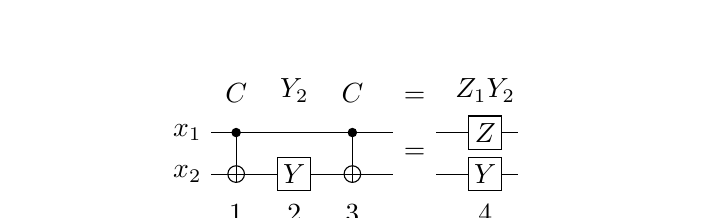
\begin{tikzpicture}[scale=1.000000,x=1pt,y=1pt]
\filldraw[color=white] (0.000000, -7.500000) rectangle (111.000000, 22.500000);
% Drawing wires
% Line 1: a1 W x_1
\draw[color=black] (0.000000,15.000000) -- (111.000000,15.000000);
\draw[color=black] (0.000000,15.000000) node[left] {$x_1$};
% Line 2: a2 W x_2
\draw[color=black] (0.000000,0.000000) -- (111.000000,0.000000);
\draw[color=black] (0.000000,0.000000) node[left] {$x_2$};
% Done with wires; drawing gates
% Line 3: a1 +a2 % $C$ % 1
\draw (9.000000, 22.500000) node[text width=144pt,above,text centered] {$C$};
\draw (9.000000, -7.500000) node[text width=144pt,below,text centered] {1};
\draw (9.000000,15.000000) -- (9.000000,0.000000);
\filldraw (9.000000, 15.000000) circle(1.500000pt);
\begin{scope}
\draw[fill=white] (9.000000, 0.000000) circle(3.000000pt);
\clip (9.000000, 0.000000) circle(3.000000pt);
\draw (6.000000, 0.000000) -- (12.000000, 0.000000);
\draw (9.000000, -3.000000) -- (9.000000, 3.000000);
\end{scope}
% Line 4: a2 G $Y$ % $Y_1$ % 2
\draw (30.000000, 22.500000) node[text width=144pt,above,text centered] {$Y_2$};
\draw (30.000000, -7.500000) node[text width=144pt,below,text centered] {2};
\begin{scope}
\draw[fill=white] (30.000000, -0.000000) +(-45.000000:8.485281pt and 8.485281pt) -- +(45.000000:8.485281pt and 8.485281pt) -- +(135.000000:8.485281pt and 8.485281pt) -- +(225.000000:8.485281pt and 8.485281pt) -- cycle;
\clip (30.000000, -0.000000) +(-45.000000:8.485281pt and 8.485281pt) -- +(45.000000:8.485281pt and 8.485281pt) -- +(135.000000:8.485281pt and 8.485281pt) -- +(225.000000:8.485281pt and 8.485281pt) -- cycle;
\draw (30.000000, -0.000000) node {$Y$};
\end{scope}
% Line 5: a1 +a2 % $C$ % 3
\draw (51.000000, 22.500000) node[text width=144pt,above,text centered] {$C$};
\draw (51.000000, -7.500000) node[text width=144pt,below,text centered] {3};
\draw (51.000000,15.000000) -- (51.000000,0.000000);
\filldraw (51.000000, 15.000000) circle(1.500000pt);
\begin{scope}
\draw[fill=white] (51.000000, 0.000000) circle(3.000000pt);
\clip (51.000000, 0.000000) circle(3.000000pt);
\draw (48.000000, 0.000000) -- (54.000000, 0.000000);
\draw (51.000000, -3.000000) -- (51.000000, 3.000000);
\end{scope}
% Line 6: = % =
\draw (73.500000, 22.500000) node[text width=144pt,above,text centered] {=};
\draw[fill=white,color=white] (66.000000, -6.000000) rectangle (81.000000, 21.000000);
\draw (73.500000, 7.500000) node {$=$};
% Line 7: a1 G  $Z$  %$Z_1Y_2$% 4
\draw (99.000000, 22.500000) node[text width=144pt,above,text centered] {$Z_1Y_2$};
\draw (99.000000, -7.500000) node[text width=144pt,below,text centered] {4};
\begin{scope}
\draw[fill=white] (99.000000, 15.000000) +(-45.000000:8.485281pt and 8.485281pt) -- +(45.000000:8.485281pt and 8.485281pt) -- +(135.000000:8.485281pt and 8.485281pt) -- +(225.000000:8.485281pt and 8.485281pt) -- cycle;
\clip (99.000000, 15.000000) +(-45.000000:8.485281pt and 8.485281pt) -- +(45.000000:8.485281pt and 8.485281pt) -- +(135.000000:8.485281pt and 8.485281pt) -- +(225.000000:8.485281pt and 8.485281pt) -- cycle;
\draw (99.000000, 15.000000) node {$Z$};
\end{scope}
% Line 8: a2 G $Y$
\begin{scope}
\draw[fill=white] (99.000000, -0.000000) +(-45.000000:8.485281pt and 8.485281pt) -- +(45.000000:8.485281pt and 8.485281pt) -- +(135.000000:8.485281pt and 8.485281pt) -- +(225.000000:8.485281pt and 8.485281pt) -- cycle;
\clip (99.000000, -0.000000) +(-45.000000:8.485281pt and 8.485281pt) -- +(45.000000:8.485281pt and 8.485281pt) -- +(135.000000:8.485281pt and 8.485281pt) -- +(225.000000:8.485281pt and 8.485281pt) -- cycle;
\draw (99.000000, -0.000000) node {$Y$};
\end{scope}
% Done with gates; drawing ending labels
% Done with ending labels; drawing cut lines and comments
% Done with comments
\end{tikzpicture}

\begin{tabular}{c|r|r|r||r} 
$\ket{x_1x_2}$ & \multicolumn{1}{c|}{1} & \multicolumn{1}{c|}{2} & \multicolumn{1}{c||}{3} & \multicolumn{1}{c}{4} \\
\hline
$\ket{00}$ & $\ket{00}$ & $i\ket{01}$ & $i\ket{01}$ & $i\ket{01}$ \\
\hline
$\ket{01}$ & $\ket{01}$ & $-i\ket{00}$ & $-i\ket{00}$ & $-i\ket{00}$ \\
\hline
$\ket{10}$ & $\ket{11}$ & $-i\ket{10}$ & $-i\ket{11}$ & $-i\ket{11}$ \\
\hline
$\ket{11}$ & $\ket{10}$ & $i\ket{11}$ & $i\ket{10}$ & $i\ket{10}$ \\
\end{tabular}
\end{center}

\begin{center}
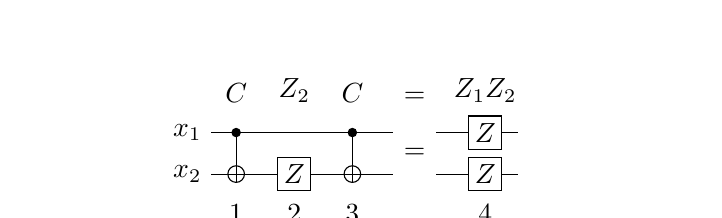
\begin{tikzpicture}[scale=1.000000,x=1pt,y=1pt]
\filldraw[color=white] (0.000000, -7.500000) rectangle (111.000000, 22.500000);
% Drawing wires
% Line 1: a1 W x_1
\draw[color=black] (0.000000,15.000000) -- (111.000000,15.000000);
\draw[color=black] (0.000000,15.000000) node[left] {$x_1$};
% Line 2: a2 W x_2
\draw[color=black] (0.000000,0.000000) -- (111.000000,0.000000);
\draw[color=black] (0.000000,0.000000) node[left] {$x_2$};
% Done with wires; drawing gates
% Line 3: a1 +a2 % $C$ % 1
\draw (9.000000, 22.500000) node[text width=144pt,above,text centered] {$C$};
\draw (9.000000, -7.500000) node[text width=144pt,below,text centered] {1};
\draw (9.000000,15.000000) -- (9.000000,0.000000);
\filldraw (9.000000, 15.000000) circle(1.500000pt);
\begin{scope}
\draw[fill=white] (9.000000, 0.000000) circle(3.000000pt);
\clip (9.000000, 0.000000) circle(3.000000pt);
\draw (6.000000, 0.000000) -- (12.000000, 0.000000);
\draw (9.000000, -3.000000) -- (9.000000, 3.000000);
\end{scope}
% Line 4: a2 G $Z$ % $Z_2$ % 2
\draw (30.000000, 22.500000) node[text width=144pt,above,text centered] {$Z_2$};
\draw (30.000000, -7.500000) node[text width=144pt,below,text centered] {2};
\begin{scope}
\draw[fill=white] (30.000000, -0.000000) +(-45.000000:8.485281pt and 8.485281pt) -- +(45.000000:8.485281pt and 8.485281pt) -- +(135.000000:8.485281pt and 8.485281pt) -- +(225.000000:8.485281pt and 8.485281pt) -- cycle;
\clip (30.000000, -0.000000) +(-45.000000:8.485281pt and 8.485281pt) -- +(45.000000:8.485281pt and 8.485281pt) -- +(135.000000:8.485281pt and 8.485281pt) -- +(225.000000:8.485281pt and 8.485281pt) -- cycle;
\draw (30.000000, -0.000000) node {$Z$};
\end{scope}
% Line 5: a1 +a2 % $C$ % 3
\draw (51.000000, 22.500000) node[text width=144pt,above,text centered] {$C$};
\draw (51.000000, -7.500000) node[text width=144pt,below,text centered] {3};
\draw (51.000000,15.000000) -- (51.000000,0.000000);
\filldraw (51.000000, 15.000000) circle(1.500000pt);
\begin{scope}
\draw[fill=white] (51.000000, 0.000000) circle(3.000000pt);
\clip (51.000000, 0.000000) circle(3.000000pt);
\draw (48.000000, 0.000000) -- (54.000000, 0.000000);
\draw (51.000000, -3.000000) -- (51.000000, 3.000000);
\end{scope}
% Line 6: = % =
\draw (73.500000, 22.500000) node[text width=144pt,above,text centered] {=};
\draw[fill=white,color=white] (66.000000, -6.000000) rectangle (81.000000, 21.000000);
\draw (73.500000, 7.500000) node {$=$};
% Line 7: a1 G  $Z$  %$Z_1Z_2$% 4
\draw (99.000000, 22.500000) node[text width=144pt,above,text centered] {$Z_1Z_2$};
\draw (99.000000, -7.500000) node[text width=144pt,below,text centered] {4};
\begin{scope}
\draw[fill=white] (99.000000, 15.000000) +(-45.000000:8.485281pt and 8.485281pt) -- +(45.000000:8.485281pt and 8.485281pt) -- +(135.000000:8.485281pt and 8.485281pt) -- +(225.000000:8.485281pt and 8.485281pt) -- cycle;
\clip (99.000000, 15.000000) +(-45.000000:8.485281pt and 8.485281pt) -- +(45.000000:8.485281pt and 8.485281pt) -- +(135.000000:8.485281pt and 8.485281pt) -- +(225.000000:8.485281pt and 8.485281pt) -- cycle;
\draw (99.000000, 15.000000) node {$Z$};
\end{scope}
% Line 8: a2 G $Z$
\begin{scope}
\draw[fill=white] (99.000000, -0.000000) +(-45.000000:8.485281pt and 8.485281pt) -- +(45.000000:8.485281pt and 8.485281pt) -- +(135.000000:8.485281pt and 8.485281pt) -- +(225.000000:8.485281pt and 8.485281pt) -- cycle;
\clip (99.000000, -0.000000) +(-45.000000:8.485281pt and 8.485281pt) -- +(45.000000:8.485281pt and 8.485281pt) -- +(135.000000:8.485281pt and 8.485281pt) -- +(225.000000:8.485281pt and 8.485281pt) -- cycle;
\draw (99.000000, -0.000000) node {$Z$};
\end{scope}
% Done with gates; drawing ending labels
% Done with ending labels; drawing cut lines and comments
% Done with comments
\end{tikzpicture}

\begin{tabular}{c|r|r|r||r} 
$\ket{x_1x_2}$ & \multicolumn{1}{c|}{1} & \multicolumn{1}{c|}{2} & \multicolumn{1}{c||}{3} & \multicolumn{1}{c}{4} \\
\hline
$\ket{00}$ & $\ket{00}$ & $\ket{00}$ & $\ket{00}$ & $\ket{00}$ \\
\hline
$\ket{01}$ & $\ket{01}$ & $-\ket{01}$ & $-\ket{01}$ & $-\ket{01}$ \\
\hline
$\ket{10}$ & $\ket{11}$ & $-\ket{11}$ & $-\ket{10}$ & $-\ket{10}$ \\
\hline
$\ket{11}$ & $\ket{10}$ & $\ket{10}$ & $\ket{11}$ & $\ket{11}$ \\
\end{tabular}
\end{center}
\noindent\rule{\textwidth}{1pt}
\begin{center}
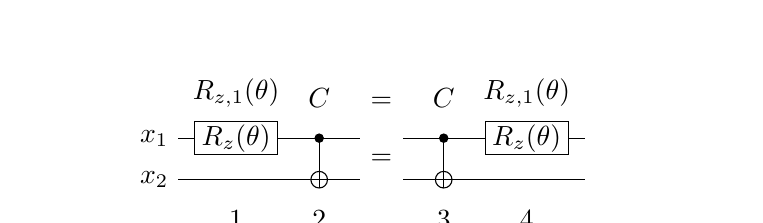
\begin{tikzpicture}[scale=1.000000,x=1pt,y=1pt]
\filldraw[color=white] (0.000000, -7.500000) rectangle (147.000000, 22.500000);
% Drawing wires
% Line 1: a1 W x_1
\draw[color=black] (0.000000,15.000000) -- (147.000000,15.000000);
\draw[color=black] (0.000000,15.000000) node[left] {$x_1$};
% Line 2: a2 W x_2
\draw[color=black] (0.000000,0.000000) -- (147.000000,0.000000);
\draw[color=black] (0.000000,0.000000) node[left] {$x_2$};
% Done with wires; drawing gates
% Line 3: a1 G $R_z(\theta)$ width=30%$R_{z,1}(\theta)$ % 1
\draw (21.000000, 22.500000) node[text width=144pt,above,text centered] {$R_{z,1}(\theta)$};
\draw (21.000000, -7.500000) node[text width=144pt,below,text centered] {1};
\begin{scope}
\draw[fill=white] (21.000000, 15.000000) +(-45.000000:21.213203pt and 8.485281pt) -- +(45.000000:21.213203pt and 8.485281pt) -- +(135.000000:21.213203pt and 8.485281pt) -- +(225.000000:21.213203pt and 8.485281pt) -- cycle;
\clip (21.000000, 15.000000) +(-45.000000:21.213203pt and 8.485281pt) -- +(45.000000:21.213203pt and 8.485281pt) -- +(135.000000:21.213203pt and 8.485281pt) -- +(225.000000:21.213203pt and 8.485281pt) -- cycle;
\draw (21.000000, 15.000000) node {$R_z(\theta)$};
\end{scope}
% Line 4: a1 +a2 % $C$ % 2
\draw (51.000000, 22.500000) node[text width=144pt,above,text centered] {$C$};
\draw (51.000000, -7.500000) node[text width=144pt,below,text centered] {2};
\draw (51.000000,15.000000) -- (51.000000,0.000000);
\filldraw (51.000000, 15.000000) circle(1.500000pt);
\begin{scope}
\draw[fill=white] (51.000000, 0.000000) circle(3.000000pt);
\clip (51.000000, 0.000000) circle(3.000000pt);
\draw (48.000000, 0.000000) -- (54.000000, 0.000000);
\draw (51.000000, -3.000000) -- (51.000000, 3.000000);
\end{scope}
% Line 5: = % $=$
\draw (73.500000, 22.500000) node[text width=144pt,above,text centered] {$=$};
\draw[fill=white,color=white] (66.000000, -6.000000) rectangle (81.000000, 21.000000);
\draw (73.500000, 7.500000) node {$=$};
% Line 6: a1 +a2 % $C$ % 3
\draw (96.000000, 22.500000) node[text width=144pt,above,text centered] {$C$};
\draw (96.000000, -7.500000) node[text width=144pt,below,text centered] {3};
\draw (96.000000,15.000000) -- (96.000000,0.000000);
\filldraw (96.000000, 15.000000) circle(1.500000pt);
\begin{scope}
\draw[fill=white] (96.000000, 0.000000) circle(3.000000pt);
\clip (96.000000, 0.000000) circle(3.000000pt);
\draw (93.000000, 0.000000) -- (99.000000, 0.000000);
\draw (96.000000, -3.000000) -- (96.000000, 3.000000);
\end{scope}
% Line 7: a1 G $R_z(\theta)$ width=30%$R_{z,1}(\theta)$ % 4
\draw (126.000000, 22.500000) node[text width=144pt,above,text centered] {$R_{z,1}(\theta)$};
\draw (126.000000, -7.500000) node[text width=144pt,below,text centered] {4};
\begin{scope}
\draw[fill=white] (126.000000, 15.000000) +(-45.000000:21.213203pt and 8.485281pt) -- +(45.000000:21.213203pt and 8.485281pt) -- +(135.000000:21.213203pt and 8.485281pt) -- +(225.000000:21.213203pt and 8.485281pt) -- cycle;
\clip (126.000000, 15.000000) +(-45.000000:21.213203pt and 8.485281pt) -- +(45.000000:21.213203pt and 8.485281pt) -- +(135.000000:21.213203pt and 8.485281pt) -- +(225.000000:21.213203pt and 8.485281pt) -- cycle;
\draw (126.000000, 15.000000) node {$R_z(\theta)$};
\end{scope}
% Done with gates; drawing ending labels
% Done with ending labels; drawing cut lines and comments
% Done with comments
\end{tikzpicture}

\begin{tabular}{c|r|r||r|r} 
$\ket{x_1x_2}$ & \multicolumn{1}{c|}{1} & \multicolumn{1}{c||}{2} & \multicolumn{1}{c|}{3} & \multicolumn{1}{c}{4} \\
\hline
$\ket{00}$ & $e^{-i\theta/2}\ket{00}$ & $e^{-i\theta/2}\ket{00}$ & $\ket{00}$ & $e^{-i\theta/2}\ket{00}$ \\
\hline
$\ket{01}$ & $e^{-i\theta/2}\ket{01}$ & $e^{-i\theta/2}\ket{01}$ & $\ket{01}$ & $e^{-i\theta/2}\ket{01}$ \\
\hline
$\ket{10}$ & $e^{i\theta/2}\ket{10}$ & $e^{i\theta/2}\ket{11}$ & $\ket{11}$ & $e^{i\theta/2}\ket{11}$ \\
\hline
$\ket{11}$ & $e^{i\theta/2}\ket{11}$ & $e^{i\theta/2}\ket{10}$ & $\ket{10}$ & $e^{i\theta/2}\ket{10}$ \\
\end{tabular}
\end{center}
\noindent\rule{\textwidth}{1pt}
\begin{center}
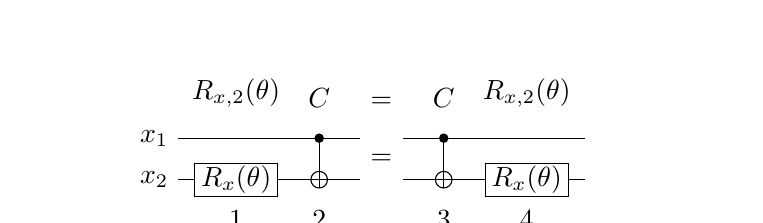
\begin{tikzpicture}[scale=1.000000,x=1pt,y=1pt]
\filldraw[color=white] (0.000000, -7.500000) rectangle (147.000000, 22.500000);
% Drawing wires
% Line 1: a1 W x_1
\draw[color=black] (0.000000,15.000000) -- (147.000000,15.000000);
\draw[color=black] (0.000000,15.000000) node[left] {$x_1$};
% Line 2: a2 W x_2
\draw[color=black] (0.000000,0.000000) -- (147.000000,0.000000);
\draw[color=black] (0.000000,0.000000) node[left] {$x_2$};
% Done with wires; drawing gates
% Line 3: a2 G $R_x(\theta)$ width=30%$R_{x,2}(\theta)$ % 1
\draw (21.000000, 22.500000) node[text width=144pt,above,text centered] {$R_{x,2}(\theta)$};
\draw (21.000000, -7.500000) node[text width=144pt,below,text centered] {1};
\begin{scope}
\draw[fill=white] (21.000000, -0.000000) +(-45.000000:21.213203pt and 8.485281pt) -- +(45.000000:21.213203pt and 8.485281pt) -- +(135.000000:21.213203pt and 8.485281pt) -- +(225.000000:21.213203pt and 8.485281pt) -- cycle;
\clip (21.000000, -0.000000) +(-45.000000:21.213203pt and 8.485281pt) -- +(45.000000:21.213203pt and 8.485281pt) -- +(135.000000:21.213203pt and 8.485281pt) -- +(225.000000:21.213203pt and 8.485281pt) -- cycle;
\draw (21.000000, -0.000000) node {$R_x(\theta)$};
\end{scope}
% Line 4: a1 +a2 % $C$ % 2
\draw (51.000000, 22.500000) node[text width=144pt,above,text centered] {$C$};
\draw (51.000000, -7.500000) node[text width=144pt,below,text centered] {2};
\draw (51.000000,15.000000) -- (51.000000,0.000000);
\filldraw (51.000000, 15.000000) circle(1.500000pt);
\begin{scope}
\draw[fill=white] (51.000000, 0.000000) circle(3.000000pt);
\clip (51.000000, 0.000000) circle(3.000000pt);
\draw (48.000000, 0.000000) -- (54.000000, 0.000000);
\draw (51.000000, -3.000000) -- (51.000000, 3.000000);
\end{scope}
% Line 5: = % $=$
\draw (73.500000, 22.500000) node[text width=144pt,above,text centered] {$=$};
\draw[fill=white,color=white] (66.000000, -6.000000) rectangle (81.000000, 21.000000);
\draw (73.500000, 7.500000) node {$=$};
% Line 6: a1 +a2 % $C$ % 3
\draw (96.000000, 22.500000) node[text width=144pt,above,text centered] {$C$};
\draw (96.000000, -7.500000) node[text width=144pt,below,text centered] {3};
\draw (96.000000,15.000000) -- (96.000000,0.000000);
\filldraw (96.000000, 15.000000) circle(1.500000pt);
\begin{scope}
\draw[fill=white] (96.000000, 0.000000) circle(3.000000pt);
\clip (96.000000, 0.000000) circle(3.000000pt);
\draw (93.000000, 0.000000) -- (99.000000, 0.000000);
\draw (96.000000, -3.000000) -- (96.000000, 3.000000);
\end{scope}
% Line 7: a2 G $R_x(\theta)$ width=30%$R_{x,2}(\theta)$ % 4
\draw (126.000000, 22.500000) node[text width=144pt,above,text centered] {$R_{x,2}(\theta)$};
\draw (126.000000, -7.500000) node[text width=144pt,below,text centered] {4};
\begin{scope}
\draw[fill=white] (126.000000, -0.000000) +(-45.000000:21.213203pt and 8.485281pt) -- +(45.000000:21.213203pt and 8.485281pt) -- +(135.000000:21.213203pt and 8.485281pt) -- +(225.000000:21.213203pt and 8.485281pt) -- cycle;
\clip (126.000000, -0.000000) +(-45.000000:21.213203pt and 8.485281pt) -- +(45.000000:21.213203pt and 8.485281pt) -- +(135.000000:21.213203pt and 8.485281pt) -- +(225.000000:21.213203pt and 8.485281pt) -- cycle;
\draw (126.000000, -0.000000) node {$R_x(\theta)$};
\end{scope}
% Done with gates; drawing ending labels
% Done with ending labels; drawing cut lines and comments
% Done with comments
\end{tikzpicture}

\begin{tabular}{c|r|r} 
$\ket{x_1x_2}$ & \multicolumn{1}{c|}{1} & \multicolumn{1}{c}{2} \\
\hline
$\ket{00}$ & $\cos(\theta/2)\ket{00}-i\sin(\theta/2)\ket{01}$ & $\cos(\theta/2)\ket{00}-i\sin(\theta/2)\ket{01}$ \\
\hline
$\ket{01}$ & $-i\sin(\theta/2)\ket{00}+\cos(\theta/2)\ket{01}$ & $-i\sin(\theta/2)\ket{00}+\cos(\theta/2)\ket{01}$ \\
\hline
$\ket{10}$ & $\cos(\theta/2)\ket{10}-i\sin(\theta/2)\ket{11}$ & $-i\sin(\theta/2)\ket{10}+\cos(\theta/2)\ket{11}$ \\
\hline
$\ket{11}$ & $-i\sin(\theta/2)\ket{10}+\cos(\theta/2)\ket{11}$ & $\cos(\theta/2)\ket{10}-i\sin(\theta/2)\ket{11}$ \\
\end{tabular}

\hspace{127.5pt}\begin{tabular}{c|r|r} 
$\ket{x_1x_2}$ & \multicolumn{1}{c|}{3} & \multicolumn{1}{c}{4} \\
\hline
$\ket{00}$ & $\ket{00}$ & $\cos(\theta/2)\ket{00}-i\sin(\theta/2)\ket{01}$ \\
\hline
$\ket{01}$ & $\ket{01}$ & $-i\sin(\theta/2)\ket{00}+\cos(\theta/2)\ket{01}$ \\
\hline
$\ket{10}$ & $\ket{11}$ & $-i\sin(\theta/2)\ket{10}+\cos(\theta/2)\ket{11}$ \\
\hline
$\ket{11}$ & $\ket{10}$ & $\cos(\theta/2)\ket{10}-i\sin(\theta/2)\ket{11}$ \\
\end{tabular}
\end{center}



%!TeX root=../solnQCQI.tex

\chapter{The quantum Fourier transform and its applications}

\Textbf{5.1} Give a direct proof that the linear transformation defined by Equation (5.2) is unitary.
$$\ket{j}\longrightarrow \sum_{k=0}^{N-1}e^{2\pi ijk/N}\ket{k}$$
\Soln First note that $e^{2\pi i/N}$ is an $N$-th root of unity, which we'll denote $\omega$.  The quantum Fourier transform (QFT) transforms $\ket{j}\rightarrow\sum_{k=0}^{N-1}\omega^{jk}\ket{k}$.  In matrix form:
$$QFT=\frac{1}{\sqrt{N}}\begin{bmatrix}1 & 1 & 1 & 1 &\ldots & 1 & 1 \\
1 & \omega^{1\cdot 1} & \omega^{2\cdot 1} & \omega^{3\cdot 1}& \ldots & \omega^{(N-2)\cdot 1} & \omega^{(N-1)\cdot 1} \\
1 & \omega^{1\cdot 2} & \omega^{2\cdot 2} & \omega^{3\cdot 2} & \ldots & \omega^{(N-2)\cdot 2} & \omega^{(N-1)\cdot 2} \\
1 & \omega^{1\cdot 3} & \omega^{2\cdot 3} & \omega^{3\cdot 3} & \ldots & \omega^{(N-2)\cdot 3} & \omega^{(N-1)\cdot 3} \\
\vdots & \vdots & \vdots & \vdots & \ddots & \vdots & \vdots \\
1 &  \omega^{1\cdot(N-2)} & \omega^{2\cdot (N-2)} & \omega^{3\cdot (N-2)} & \ldots & \omega^{(N-2)\cdot (N-2)} & \omega^{(N-1)\cdot (N-2)} \\
1 &  \omega^{1\cdot(N-1)} & \omega^{2\cdot (N-1)} & \omega^{3\cdot (N-1)} & \ldots & \omega^{(N-2)\cdot (N-1)} & \omega^{(N-1)\cdot (N-1)} \\
\end{bmatrix}$$
Noting that $\omega^* = \omega^{-1}$, we have
$$QFT^\dagger=\frac{1}{\sqrt{N}}\begin{bmatrix}1 & 1 & 1 & 1 &\ldots & 1 & 1 \\
1 & \omega^{-1\cdot 1} & \omega^{-1\cdot2} & \omega^{-1\cdot 3}& \ldots & \omega^{-1\cdot(N-2)} & \omega^{-1\cdot(N-1)} \\
1 & \omega^{-2\cdot1} & \omega^{-2\cdot 2} & \omega^{-2\cdot 3} & \ldots & \omega^{-2\cdot(N-2)} & \omega^{-2\cdot(N-1)} \\
1 & \omega^{-3\cdot1} & \omega^{-3\cdot2} & \omega^{-3\cdot 3} & \ldots &  \omega^{-3\cdot(N-2)} & \omega^{-3\cdot(N-1)} \\
\vdots & \vdots & \vdots & \vdots & \ddots & \vdots & \vdots \\
1 &  \omega^{-(N-2)\cdot 1} & \omega^{-(N-2)\cdot 2} & \omega^{-(N-2)\cdot 3} & \ldots & \omega^{-(N-2)\cdot (N-2)} & \omega^{-(N-2)\cdot (N-1)} \\
1 &  \omega^{-(N-1)\cdot 1} & \omega^{-(N-1)\cdot 2} & \omega^{-(N-1)\cdot 3} & \ldots & \omega^{-(N-1)\cdot (N-2)} & \omega^{-(N-1)\cdot (N-1)} \\
\end{bmatrix}$$
Now $QFT*QFT^\dagger=\frac{1}{N}\begin{bmatrix}\sum_{\ell=0}^{N-1} \omega^{\ell j}\omega^{-k\ell}\end{bmatrix}_{j,k} =\frac{1}{N} \begin{bmatrix}\sum_{\ell=0}^{N-1} \omega^{\ell (j-k)}\end{bmatrix}_{j,k}$.  When $j=k$, \textit{i.e.} on the diagonal, all exponents in the summation formula for the $j,k$ entry become 0, producing a sum of $N$ 1s, canceling the $\frac{1}{N}$ scalar and giving that the diagonal entries of $QFT*QFT^\dagger$ are all 1s.  For off-diagonal entries, \textit{i.e.} when $j\neq k$, let $a=j-k$.  Recognizing a finite geometric series and that $\omega$ is an $N$-th root of unity, we have:
$$\sum_{\ell=0}^{N-1} \omega^{\ell (j-k)} = \sum_{\ell=0}^{N-1} \omega^{a\cdot\ell} = 1+\omega^a+\omega^{2a}+\ldots+\omega^{(N-1)a} = \frac{1-\omega^{N\cdot a}}{1-\omega^a} = \frac{1-1^a}{1-\omega^a}= 0$$
Note that the denominator is non-zero, since $a\neq 0$.  Ultimately, $QFT*QFT^\dagger=I$, and $QFT$ is unitary.

\Textbf{5.2} Explicitly compute the Fourier transform of the $n$ qubit state $\ket{00\ldots0}$.
\Soln $QFT(\ket{00\ldots0})=\frac{1}{2^{n-1}}\sum_{k=0}^{\sqrt{2^n}}\ket{k}$.
\Textbf{5.3}
\Textbf{5.4} Give a decomposition of the controlled-$R_k$ gate into single qubit and \CNOT\ gates.
\Soln By Theorem 4.1 we may write $R_k=e^{i\alpha}R_z(\beta)R_y(\gamma)R_z(\delta)$ for some $\alpha, \beta, \gamma$ and $\delta$.  In this case, $\alpha=2\pi/2^{k+1}$, $\beta=0$, $\gamma=0$, and $\delta=2\pi/2^k$ suffice, since 
\begin{align*}
e^{2i\pi/2^{k+1}}R_z(0)R_y(0)R_z(2\pi/2^k)&=e^{2i\pi/2^{k+1}}I^2\begin{bmatrix}e^{-2i\pi/2^{k+1}} & 0 \\ 0 & e^{2i\pi/2^{k+1}}\end{bmatrix}
&=\begin{bmatrix}1 & 0 \\ 0 & e^{2i\pi/2^k}\end{bmatrix}=R_k\
\end{align*}
Following the proof of Corollary 4.2, set $A=R_z(0)R_y(0)=I, B=R_y(0)R_z(-2\pi/2^{k+1})=R_z(-2\pi/2^{k+1}),  C=R_z(2\pi/2^{k+1})$ so that $ABC=I$ and $U=e^{i\alpha}AXBXC$.  Applying the construction in Figure 4.6 gives:
\begin{center}
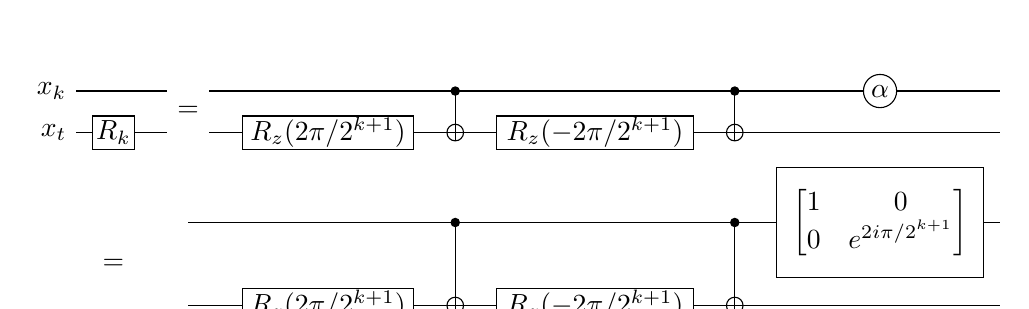
\begin{tikzpicture}[scale=1.000000,x=1pt,y=1pt]
\filldraw[color=white] (0.000000, -5.000000) rectangle (334.000000, 85.000000);
% Drawing wires
% Line 1: a1 W x_k
\draw[color=black] (0.000000,77.500000) -- (334.000000,77.500000);
\draw[color=black] (0.000000,77.500000) node[left] {$x_k$};
% Line 2: a2 W x_t
\draw[color=black] (0.000000,62.500000) -- (334.000000,62.500000);
\draw[color=black] (0.000000,62.500000) node[left] {$x_t$};
% Line 3: a3 W  breadth=50
\draw[color=black] (40.500000,30.000000) -- (334.000000,30.000000);
% Line 4: a4 W breadth=10
\draw[color=black] (40.500000,0.000000) -- (334.000000,0.000000);
% Done with wires; drawing gates
% Line 5: a2 G $R_k$ width=15
\begin{scope}
\draw[fill=white] (13.500000, 62.500000) +(-45.000000:10.606602pt and 8.485281pt) -- +(45.000000:10.606602pt and 8.485281pt) -- +(135.000000:10.606602pt and 8.485281pt) -- +(225.000000:10.606602pt and 8.485281pt) -- cycle;
\clip (13.500000, 62.500000) +(-45.000000:10.606602pt and 8.485281pt) -- +(45.000000:10.606602pt and 8.485281pt) -- +(135.000000:10.606602pt and 8.485281pt) -- +(225.000000:10.606602pt and 8.485281pt) -- cycle;
\draw (13.500000, 62.500000) node {$R_k$};
\end{scope}
% Line 7: a3 a4 =
\draw[fill=white,color=white] (6.000000, -6.000000) rectangle (21.000000, 36.000000);
\draw (13.500000, 15.000000) node {$=$};
% Line 6: a1 a2 =
\draw[fill=white,color=white] (33.000000, 56.500000) rectangle (48.000000, 83.500000);
\draw (40.500000, 70.000000) node {$=$};
% Line 8: a3 START
% Line 9: a4 START
% Line 10: a2 G $R_z(2\pi/2^{k+1})$ width=62
\begin{scope}
\draw[fill=white] (91.000000, 62.500000) +(-45.000000:43.840620pt and 8.485281pt) -- +(45.000000:43.840620pt and 8.485281pt) -- +(135.000000:43.840620pt and 8.485281pt) -- +(225.000000:43.840620pt and 8.485281pt) -- cycle;
\clip (91.000000, 62.500000) +(-45.000000:43.840620pt and 8.485281pt) -- +(45.000000:43.840620pt and 8.485281pt) -- +(135.000000:43.840620pt and 8.485281pt) -- +(225.000000:43.840620pt and 8.485281pt) -- cycle;
\draw (91.000000, 62.500000) node {$R_z(2\pi/2^{k+1})$};
\end{scope}
% Line 15: a4 G $R_z(2\pi/2^{k+1})$ width=62
\begin{scope}
\draw[fill=white] (91.000000, -0.000000) +(-45.000000:43.840620pt and 8.485281pt) -- +(45.000000:43.840620pt and 8.485281pt) -- +(135.000000:43.840620pt and 8.485281pt) -- +(225.000000:43.840620pt and 8.485281pt) -- cycle;
\clip (91.000000, -0.000000) +(-45.000000:43.840620pt and 8.485281pt) -- +(45.000000:43.840620pt and 8.485281pt) -- +(135.000000:43.840620pt and 8.485281pt) -- +(225.000000:43.840620pt and 8.485281pt) -- cycle;
\draw (91.000000, -0.000000) node {$R_z(2\pi/2^{k+1})$};
\end{scope}
% Line 11: a1 +a2
\draw (137.000000,77.500000) -- (137.000000,62.500000);
\filldraw (137.000000, 77.500000) circle(1.500000pt);
\begin{scope}
\draw[fill=white] (137.000000, 62.500000) circle(3.000000pt);
\clip (137.000000, 62.500000) circle(3.000000pt);
\draw (134.000000, 62.500000) -- (140.000000, 62.500000);
\draw (137.000000, 59.500000) -- (137.000000, 65.500000);
\end{scope}
% Line 16: a3 +a4
\draw (137.000000,30.000000) -- (137.000000,0.000000);
\filldraw (137.000000, 30.000000) circle(1.500000pt);
\begin{scope}
\draw[fill=white] (137.000000, 0.000000) circle(3.000000pt);
\clip (137.000000, 0.000000) circle(3.000000pt);
\draw (134.000000, 0.000000) -- (140.000000, 0.000000);
\draw (137.000000, -3.000000) -- (137.000000, 3.000000);
\end{scope}
% Line 12: a2 G $R_z(-2\pi/2^{k+1})$ width=71
\begin{scope}
\draw[fill=white] (187.500000, 62.500000) +(-45.000000:50.204581pt and 8.485281pt) -- +(45.000000:50.204581pt and 8.485281pt) -- +(135.000000:50.204581pt and 8.485281pt) -- +(225.000000:50.204581pt and 8.485281pt) -- cycle;
\clip (187.500000, 62.500000) +(-45.000000:50.204581pt and 8.485281pt) -- +(45.000000:50.204581pt and 8.485281pt) -- +(135.000000:50.204581pt and 8.485281pt) -- +(225.000000:50.204581pt and 8.485281pt) -- cycle;
\draw (187.500000, 62.500000) node {$R_z(-2\pi/2^{k+1})$};
\end{scope}
% Line 17: a4 G $R_z(-2\pi/2^{k+1})$ width=71
\begin{scope}
\draw[fill=white] (187.500000, -0.000000) +(-45.000000:50.204581pt and 8.485281pt) -- +(45.000000:50.204581pt and 8.485281pt) -- +(135.000000:50.204581pt and 8.485281pt) -- +(225.000000:50.204581pt and 8.485281pt) -- cycle;
\clip (187.500000, -0.000000) +(-45.000000:50.204581pt and 8.485281pt) -- +(45.000000:50.204581pt and 8.485281pt) -- +(135.000000:50.204581pt and 8.485281pt) -- +(225.000000:50.204581pt and 8.485281pt) -- cycle;
\draw (187.500000, -0.000000) node {$R_z(-2\pi/2^{k+1})$};
\end{scope}
% Line 13: a1 +a2
\draw (238.000000,77.500000) -- (238.000000,62.500000);
\filldraw (238.000000, 77.500000) circle(1.500000pt);
\begin{scope}
\draw[fill=white] (238.000000, 62.500000) circle(3.000000pt);
\clip (238.000000, 62.500000) circle(3.000000pt);
\draw (235.000000, 62.500000) -- (241.000000, 62.500000);
\draw (238.000000, 59.500000) -- (238.000000, 65.500000);
\end{scope}
% Line 18: a3 +a4
\draw (238.000000,30.000000) -- (238.000000,0.000000);
\filldraw (238.000000, 30.000000) circle(1.500000pt);
\begin{scope}
\draw[fill=white] (238.000000, 0.000000) circle(3.000000pt);
\clip (238.000000, 0.000000) circle(3.000000pt);
\draw (235.000000, 0.000000) -- (241.000000, 0.000000);
\draw (238.000000, -3.000000) -- (238.000000, 3.000000);
\end{scope}
% Line 14: a1 P $\alpha$
\begin{scope}
\draw[fill=white] (290.500000, 77.500000) circle(6.000000pt);
\clip (290.500000, 77.500000) circle(6.000000pt);
\draw (290.500000, 77.500000) node {$\alpha$};
\end{scope}
% Line 19: a3 G $\begin{bmatrix}1 & 0 \\ 0 & e^{2i\pi/2^{k+1}}\end{bmatrix}$ height=40 width=75
\begin{scope}
\draw[fill=white] (290.500000, 30.000000) +(-45.000000:53.033009pt and 28.284271pt) -- +(45.000000:53.033009pt and 28.284271pt) -- +(135.000000:53.033009pt and 28.284271pt) -- +(225.000000:53.033009pt and 28.284271pt) -- cycle;
\clip (290.500000, 30.000000) +(-45.000000:53.033009pt and 28.284271pt) -- +(45.000000:53.033009pt and 28.284271pt) -- +(135.000000:53.033009pt and 28.284271pt) -- +(225.000000:53.033009pt and 28.284271pt) -- cycle;
\draw (290.500000, 30.000000) node {$\begin{bmatrix}1 & 0 \\ 0 & e^{2i\pi/2^{k+1}}\end{bmatrix}$};
\end{scope}
% Done with gates; drawing ending labels
% Done with ending labels; drawing cut lines and comments
% Done with comments
\end{tikzpicture}
\end{center}
\Textbf{5.5} Give a quantum circuit to perform the inverse quantum Fourier transform.
\Soln The inverse quantum Fourier transform is the $QFT^\dagger$ transformation shown in Exercise 5.1.  For a fixed computational basis state $\ket{k}$, 
\begin{align*}
QFT^\dagger(\ket{k})&=\frac{1}{\sqrt{N}}\sum_{j=0}^{N-1}e^{-2\pi ijk/2^n}\ket{j} \\
&=\frac{\Bigl(\ket{0}+e^{-2\pi i0.k_n}\ket{1}\Bigr)\Bigl(\ket{0}+e^{-2\pi i0.k_{n-1}k_n}\ket{1}\Bigr)\cdots\Bigl(\ket{0}+e^{-2\pi i0.k_1k_2\ldots k_{n-1}k_n}\ket{1}\Bigr)}{\sqrt{N}}
\end{align*}
Using $R_\ell^{\dagger}=\begin{bmatrix}1 & 0 \\ 0 & e^{-2\pi i/2^{\ell}}\end{bmatrix}$ instead of $R_\ell$ in Figure 5.1 will implement $QFT^\dagger$.  It's verification is effectively identical to that of Figure 5.1 on page 219.  For completeness, the circuit is diagrammed here:

\begin{center}
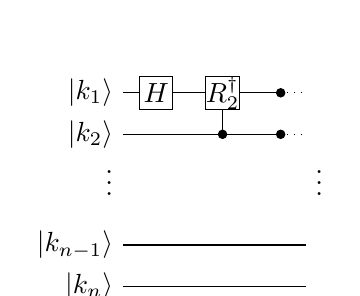
\begin{tikzpicture}[scale=1.000000,x=1pt,y=1pt]
\filldraw[color=white] (0.000000, -7.500000) rectangle (66.000000, 77.500000);
% Drawing wires
% Line 3: a1 W  \ket{k_1}
\draw[color=black] (0.000000,70.000000) -- (57.000000,70.000000);
\draw[color=black,dotted] (57.000000,70.000000) -- (66.000000,70.000000);
\draw[color=black] (0.000000,70.000000) node[left] {$\ket{k_1}$};
% Line 4: a2 W  \ket{k_2}
\draw[color=black] (0.000000,55.000000) -- (57.000000,55.000000);
\draw[color=black,dotted] (57.000000,55.000000) -- (66.000000,55.000000);
\draw[color=black] (0.000000,55.000000) node[left] {$\ket{k_2}$};
% Line 5: ...b W breadth=25
\draw[color=black] (0.000000,35.000000) node[anchor=mid east] {$\vdots$};
% Line 6: km W \ket{k_{n-1}}
\draw[color=black] (0.000000,15.000000) -- (66.000000,15.000000);
\draw[color=black] (0.000000,15.000000) node[left] {$\ket{k_{n-1}}$};
% Line 7: kn W \ket{k_n}
\draw[color=black] (0.000000,0.000000) -- (66.000000,0.000000);
\draw[color=black] (0.000000,0.000000) node[left] {$\ket{k_n}$};
% Done with wires; drawing gates
% Line 8: a1 H
\begin{scope}
\draw[fill=white] (12.000000, 70.000000) +(-45.000000:8.485281pt and 8.485281pt) -- +(45.000000:8.485281pt and 8.485281pt) -- +(135.000000:8.485281pt and 8.485281pt) -- +(225.000000:8.485281pt and 8.485281pt) -- cycle;
\clip (12.000000, 70.000000) +(-45.000000:8.485281pt and 8.485281pt) -- +(45.000000:8.485281pt and 8.485281pt) -- +(135.000000:8.485281pt and 8.485281pt) -- +(225.000000:8.485281pt and 8.485281pt) -- cycle;
\draw (12.000000, 70.000000) node {$H$};
\end{scope}
% Line 9: a1 G $R_2$ a2
\draw (36.000000,70.000000) -- (36.000000,55.000000);
\begin{scope}
\draw[fill=white] (36.000000, 70.000000) +(-45.000000:8.485281pt and 8.485281pt) -- +(45.000000:8.485281pt and 8.485281pt) -- +(135.000000:8.485281pt and 8.485281pt) -- +(225.000000:8.485281pt and 8.485281pt) -- cycle;
\clip (36.000000, 70.000000) +(-45.000000:8.485281pt and 8.485281pt) -- +(45.000000:8.485281pt and 8.485281pt) -- +(135.000000:8.485281pt and 8.485281pt) -- +(225.000000:8.485281pt and 8.485281pt) -- cycle;
\draw (36.000000, 70.000000) node {$R_2^\dagger$};
\end{scope}
\filldraw (36.000000, 55.000000) circle(1.500000pt);
% Line 10: a1:dot
\filldraw (57.000000, 70.000000) circle(1.500000pt);
% Line 11: a2:dot
\filldraw (57.000000, 55.000000) circle(1.500000pt);
% Done with gates; drawing ending labels
\draw[color=black] (66.000000,35.000000) node[anchor=mid west] {$\vdots$};
% Done with ending labels; drawing cut lines and comments
% Done with comments
\end{tikzpicture}
\end{center}

\Textbf{5.6} \textbf{(Approximate quantum Fourier transform)}  The quantum circuit construction of the quantum Fourier transform apparently requires gates of exponential precision in the number of qubits used.  However, such precision is never required in any quantum circuit of polynomial size.  For example, let $U$ be the ideal quantum Fourier transform on $n$ qubits, and $V$ be the transform which results if the controlled $R_k$ gates are performed to a precision of $\Delta = 1/p(n)$ for some polynomial $p(n)$.  Show that the error $E(U,V)=\max_{\ket{\psi}}\norm{(U-V)\ket{\psi}}$ scales as $\Theta(n^2/p(n))$, and thus polynomial precision in each gate is sufficient to guarantee polynomial accuracy in the output state.
\Soln 
Let $R^i_j$ be the controlled $R_j$ gate, controlled by the qubit with index $j$ in Figure 5.1 (1-up), targeting the qubit with index $i$.  Let $R'^i_j$ be the same gate performed with precision to a precision of $\Delta$.  Note that the superscripts indicate the target and are not exponents.
\begin{align*}
E(U,V) &\equiv \max_{\ket{\psi}}\norm{(U-V)\ket{\psi}} \tag{definition} \\
&= \max_{\ket{\psi}}\ \Bigl|\Bigl|(H^1R^1_2R^1_3\cdots R^1_n H^2R^2_2\cdots R^2_{n-1}\cdots H^{n-1}R^{n-1}_2 H^n \\
&\ \ \ \ \ \ \ \ \ \ \ -H^1R'^1_2R'^1_3\cdots R'^1_n H^2R'^2_2\cdots R'^2_{n-1}\cdots H^{n-1}R'^{n-1}_2 H^n)\ket{\psi}\Bigr|\Bigr|
\end{align*}
The trick seems to be to apply a (supposedly true) lemma that $E(AB,A'B') \leq E(A,A')+E(B,B')$. This doesn't seem to be entirely obvious, but if allowed to apply it:
\begin{align*}
&\leq E(H^1, H^1) + E(R_2^1,R'^1_2) + \ldots + E(R_n^1, R'^1_n) + E(H^2, H^2) \\
&\ \ \ \ + E(R_2^2,R'^2_2) + \ldots + E(R_{n-1}^2, R'^2_{n-1}) +\ldots \\
&\ \ \ \ + E(H^{n-1}, H^{n-1}) + E(R^{n-1}_2, R'^{n-1}_2) + E(H^n,H^n) \\
&\leq 0+\Delta + \ldots + \Delta + 0 + \Delta +\ldots + \Delta + \ldots + 0 + \Delta + 0 \\
&= (n-1)\Delta + (n-2)\Delta + \ldots + \Delta \\
&= \Delta\sum_{i=1}^{n-1} i \\
&= \left(\frac{n(n-1)}{2}\right)\delta \leq \frac{n*(n-1)}{2p(n)} = O(n^2/p(n))
\end{align*}
This only gives an upper bound.  A lower bound is less important and would seem to require a lower bound in the lemma, which I'm suspicious of.  It would also require the assumption that the controlled $R_k$ gates are performed with causal error $\Delta$.  In practice, this is unlikely to be the case.  In application, the only causal errors are likely to be the result of simply not performing the controlled-$R_k$ gates at all, for $k$ above some fixed threshold.  Doing so would introduce causal errors, but those errors would depend on $k$, not $n$. The threshold for $k$ may depend on $n$, and the \textit{total} error depends on the number of controlled-$R_k$ gates not performed which is determined by $n$, but individually the error in not performing a single controlled-$R_k$ would depend only on $k$.

\Textbf{5.7} Additional insight into the circuit in Figure 5.2 amy be obtained by showing, as you should now do, that the effect of the sequence of controlled-$U$ operations like that in Figure 5.2 is to take the state $\ket{j}\ket{u}$ to $\ket{j}U^j\ket{u}$. (Note that this does not depend on $\ket{u}$ being an eigenstate of $U$.
\Soln Note that $\ket{j}$ is implicitly assumed to be a computational basis state, so let's write $j = j_{t-1}j_{t-2}\ldots j_1j_0$ in binary.  Preferring to write quantum registers in big-endian: $\ket{j}=\ket{j_0j_1\ldots j_{t-2}j_{t-1}}$.  The sequence of controlled-$U$ gates is thus:
\begin{center}
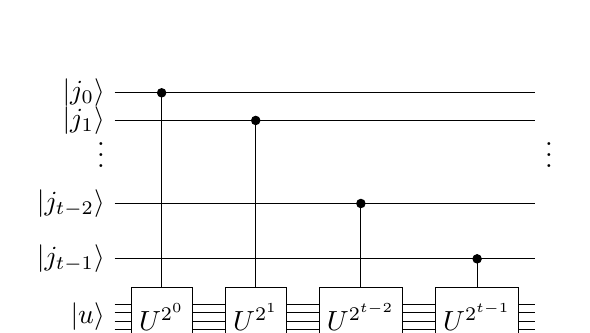
\begin{tikzpicture}[scale=1.000000,x=1pt,y=1pt]
\filldraw[color=white] (0.000000, -1.500000) rectangle (152.000000, 90.500000);
% Drawing wires
% Line 1: a0 W \ket{j_0} breadth=10
\draw[color=black] (0.000000,85.500000) -- (152.000000,85.500000);
\draw[color=black] (0.000000,85.500000) node[left] {$\ket{j_0}$};
% Line 2: a1 W \ket{j_1} breadth=10
\draw[color=black] (0.000000,75.500000) -- (152.000000,75.500000);
\draw[color=black] (0.000000,75.500000) node[left] {$\ket{j_1}$};
% Line 3: ...b W breadth=20
\draw[color=black] (0.000000,60.500000) node[anchor=mid east] {$\vdots$};
% Line 4: at2 W \ket{j_{t-2}} breadth=10
\draw[color=black] (0.000000,45.500000) -- (152.000000,45.500000);
\draw[color=black] (0.000000,45.500000) node[left] {$\ket{j_{t-2}}$};
% Line 5: at1 W \ket{j_{t-1}} breadth=30
\draw[color=black] (0.000000,25.500000) -- (152.000000,25.500000);
\draw[color=black] (0.000000,25.500000) node[left] {$\ket{j_{t-1}}$};
% Line 6: t1 t2 t3 t4 W \ket{u} breadth=3
\draw[color=black] (0.000000,9.000000) -- (152.000000,9.000000);
%   Deferring wire label at (0.000000,9.000000)
% Line 6: t1 t2 t3 t4 W \ket{u} breadth=3
\draw[color=black] (0.000000,6.000000) -- (152.000000,6.000000);
%   Deferring wire label at (0.000000,6.000000)
% Line 6: t1 t2 t3 t4 W \ket{u} breadth=3
\draw[color=black] (0.000000,3.000000) -- (152.000000,3.000000);
%   Deferring wire label at (0.000000,3.000000)
% Line 6: t1 t2 t3 t4 W \ket{u} breadth=3
\draw[color=black] (0.000000,0.000000) -- (152.000000,0.000000);
\draw[color=black] (0.000000,4.500000) node[left] {$\ket{u}$};
% Done with wires; drawing gates
% Line 7: t1 t2 t3 t4 G $U^{2^0}$ a0 width=22 height=16
\draw (17.000000,85.500000) -- (17.000000,0.000000);
\begin{scope}
\draw[fill=white] (17.000000, 4.500000) +(-45.000000:15.556349pt and 14.849242pt) -- +(45.000000:15.556349pt and 14.849242pt) -- +(135.000000:15.556349pt and 14.849242pt) -- +(225.000000:15.556349pt and 14.849242pt) -- cycle;
\clip (17.000000, 4.500000) +(-45.000000:15.556349pt and 14.849242pt) -- +(45.000000:15.556349pt and 14.849242pt) -- +(135.000000:15.556349pt and 14.849242pt) -- +(225.000000:15.556349pt and 14.849242pt) -- cycle;
\draw (17.000000, 4.500000) node {$U^{2^0}$};
\end{scope}
\filldraw (17.000000, 85.500000) circle(1.500000pt);
% Line 8: t1 t2 t3 t4 G $U^{2^1}$ a1 width=22 height=16
\draw (51.000000,75.500000) -- (51.000000,0.000000);
\begin{scope}
\draw[fill=white] (51.000000, 4.500000) +(-45.000000:15.556349pt and 14.849242pt) -- +(45.000000:15.556349pt and 14.849242pt) -- +(135.000000:15.556349pt and 14.849242pt) -- +(225.000000:15.556349pt and 14.849242pt) -- cycle;
\clip (51.000000, 4.500000) +(-45.000000:15.556349pt and 14.849242pt) -- +(45.000000:15.556349pt and 14.849242pt) -- +(135.000000:15.556349pt and 14.849242pt) -- +(225.000000:15.556349pt and 14.849242pt) -- cycle;
\draw (51.000000, 4.500000) node {$U^{2^1}$};
\end{scope}
\filldraw (51.000000, 75.500000) circle(1.500000pt);
% Line 9: t1 t2 t3 t4 G $U^{2^{t-2}}$ at2 width=30 height=16
\draw (89.000000,45.500000) -- (89.000000,0.000000);
\begin{scope}
\draw[fill=white] (89.000000, 4.500000) +(-45.000000:21.213203pt and 14.849242pt) -- +(45.000000:21.213203pt and 14.849242pt) -- +(135.000000:21.213203pt and 14.849242pt) -- +(225.000000:21.213203pt and 14.849242pt) -- cycle;
\clip (89.000000, 4.500000) +(-45.000000:21.213203pt and 14.849242pt) -- +(45.000000:21.213203pt and 14.849242pt) -- +(135.000000:21.213203pt and 14.849242pt) -- +(225.000000:21.213203pt and 14.849242pt) -- cycle;
\draw (89.000000, 4.500000) node {$U^{2^{t-2}}$};
\end{scope}
\filldraw (89.000000, 45.500000) circle(1.500000pt);
% Line 10: t1 t2 t3 t4 G $U^{2^{t-1}}$ at1 width=30 height=16
\draw (131.000000,25.500000) -- (131.000000,0.000000);
\begin{scope}
\draw[fill=white] (131.000000, 4.500000) +(-45.000000:21.213203pt and 14.849242pt) -- +(45.000000:21.213203pt and 14.849242pt) -- +(135.000000:21.213203pt and 14.849242pt) -- +(225.000000:21.213203pt and 14.849242pt) -- cycle;
\clip (131.000000, 4.500000) +(-45.000000:21.213203pt and 14.849242pt) -- +(45.000000:21.213203pt and 14.849242pt) -- +(135.000000:21.213203pt and 14.849242pt) -- +(225.000000:21.213203pt and 14.849242pt) -- cycle;
\draw (131.000000, 4.500000) node {$U^{2^{t-1}}$};
\end{scope}
\filldraw (131.000000, 25.500000) circle(1.500000pt);
% Done with gates; drawing ending labels
\draw[color=black] (152.000000,60.500000) node[anchor=mid west] {$\vdots$};
% Done with ending labels; drawing cut lines and comments
% Done with comments
\end{tikzpicture}
\end{center}
with each $\ket{j_s}$ being either $\ket{0}$ or $\ket{1}$.  The controlled $U^{2^s}$ gate is applied to $\ket{u}$ if and only if $\ket{j_s} = \ket{1}$ which can be represented by multiplication of $\ket{u}$ by $U^{j_s2^s}$.
\begin{align*}
\ket{j}\ket{u} &= \ket{j_0j_1\ldots j_{t-2}j_{t-1}}\ket{u} \\
&\rightarrow \ket{j_0j_1\ldots j_{t-2}j_{t-1}}  U^{j_{t-1}2^{t-1}}U^{j_{t-2}2^{t-2}}\cdots U^{j_12^1}U^{j_02^0}\ket{u}\\
&= \ket{j_0j_1\ldots j_{t-2}j_{t-1}} U^{j_0j_1\ldots j_{t-2}j_{t-1}}\ket{u}  \tag{collect powers of $U$ in binary}\\
&= \ket{j}U^j\ket{u} \tag{recognize binary representation of $j$}
\end{align*}

\Textbf{5.8} Suppose the phase estimation algorithm takes the state $\ket{0}\ket{u}$ to the state $\ket{\widetilde{\varphi_u}}\ket{u}$, so that given then input $\ket{0}(\sum_uc_u\ket{u})$, the algorithm outputs $\sum_uc_u\ket{\widetilde{\varphi_u}}\ket{u}$.  Show that is $t$ is chosen according to (5.35), then the probability for measuring $\varphi_u$ accurate to $n$ bits at the conclusion of the phase estimation algorithm is at least $|c_u|^2(1-\epsilon)$.
\Soln Note that in this problem we assume $\{\ket{u}\}$ forms an eigenbasis, but that the bound on probability is requested for measuring $\varphi_u$ for some fixed eigenvalue, say $\upsilon$.  Measurement of the second register collapses the state  to $\ket{\widetilde\varphi_{\upsilon}}\ket{\upsilon}$ with probabily $|c_{\upsilon}|^2$, from which we can determine $\varphi_{\upsilon}$ accurate to $n$ bits with probability $1-\epsilon$.  Multiplying probabilities gives that performing phase estimation on $\ket{0}(\sum_uc_u\ket{u})$ gives a probability of measuring $\varphi_{\upsilon}$ accurate to $n$ bits of $|c_\upsilon|^2(1-\epsilon)$. 

\Textbf{5.9}
\Textbf{5.10} Show that the (multiplicative) order of $(x=)5$ mod $(N=)21$ is $6$.
\Soln It suffices to show that $5^t \not\equiv 1 \pmod{21}$ for $1\leq t < 5$, and that $5^6 \equiv 1 \pmod{21}$
\begin{center}
\begin{tabular}{|c|c|}
\hline
$t$ & $5^t \pmod{21}$ \\
\hline
\hline
0 & 1 \\
\hline
1 & 5 \\
\hline
2 & 4 \\
\hline
3 & 20 $(\equiv -1)$ \\
\hline
4 & 16 $(\equiv -5)$ \\
\hline
5 & 17 $(\equiv -4)$ \\
\hline
\hline
6 & 1 $(\equiv -20)$ \\
\hline
\end{tabular}
\end{center}

\Textbf{5.11} Show that the (multiplicative) order of $x$ (mod $N$) satisfies $r \leq N$.
\Soln Note that $x\neq 0$, since $0^r \equiv 0 \pmod{N}$ for all $r$, and the order of $1$ is $1$ for all $N$.  For $N\geq 2$, see Euler's totient theorem which states that when $\gcd(x,N)=1$, $x^{\phi(N)}\equiv 1 \pmod{N}$, where $\phi(N)$ is the totient of $N$, \textit{i.e.} the number of integers $1\leq n \leq N$ such that $\gcd(n,N) = 1$.  For $N\geq 2$, $\gcd(N,N) \neq 1$, so $\phi(N) \leq N-1$.  Equality holds (for $\phi$ and the order of $x$) if and only if $N$ is prime.  In the end, for $N \geq 2$, the order of any integer $x$ comprime to the modulus $N$ is at most $\phi(N) \leq N-1$.  Note, with a little additional consideration it can be shown that the order of $x$ is, in fact, a divisor $\phi(N)$ by using Lagrange's Theorem on subgroup orders applied to the cyclic group generated by $x$ in the multiplicative group mod $N$.

\Textbf{5.12} Show that $U$ is unitary (\textit{Hint:} $x$ is co-prime to $N$, and therefore has an inverse modulo $N$)
\Soln $U$ performs modular multiplication by $x$.  When $x$ is coprime to $N$, modular multiplication by $x$ executes a permutation of the computational basis states, that is, $U$ is a permutation matrix.  Inverses of permutation matrices are easily seen to be their transposes.  So, $U^\dagger U = U^TU = U^{-1}U = I$, and $U$ is unitary.

\Textbf{5.13} Prove (5.44): $$\frac{1}{\sqrt{r}}\sum_{s=0}^{r-1}\ket{u_s} = \ket{1}.$$ (\textit{Hint:} $\sum_{s=0}^{r-1}\exp(-2\pi isk/r) = r\delta_{k0}$.)  In fact, prove that $$\frac{1}{\sqrt{r}}\sum_{s=0}^{r-1}e^{2\pi isk/r}\ket{u_s} = \ket{x^k\hspace{-10pt}\pmod{N}}.$$
\Soln Note that in this exercise $k$ is fixed, whereas in the definition of $\ket{u_s}$ in equation (5.37), $k$ is an index that is iterated over.  Below, we'll iterate over $k'$ instead of $k$.  In the hint, $k$ is arbitrary.  We'll apply it to $(k-k')$ at a point at which $k'$ will also be fixed, yielding $\sum_{s=0}^{r-1}\exp(-2\pi is(k-k')/r) = r\delta_{(k-k')0}=r\delta_{kk'}$.
\begin{align*}
\frac{1}{\sqrt{r}}\sum_{s=0}^{r-1}e^{2\pi isk/r}\ket{u_s} &= \frac{1}{\sqrt{r}}\sum_{s=0}^{r-1}e^{2\pi isk/r}\left(\frac{1}{\sqrt{r}}\sum_{k'=0}^{r-1}e^{-2\pi isk'/r}\ket{x^{k'}\hspace{-10pt}\pmod{N}}\right)\\
&= \frac{1}{r}\sum_{s=0}^{r-1}\sum_{k'=0}^{r-1}e^{2\pi is(k-k')/r}\ket{x^{k'}\hspace{-10pt}\pmod{N}} \tag{distribute} \\
&= \frac{1}{r}\sum_{k'=0}^{r-1}\left(\sum_{s=0}^{r-1}e^{2\pi is(k-k')/r}\right)\ket{x^{k'}\hspace{-10pt}\pmod{N}} \tag{change order} \\
&= \frac{1}{r}\sum_{k'=0}^{r-1}r\delta_{kk'}\ket{x^{k'}\hspace{-10pt}\pmod{N}} \tag{apply hint} \\
&= \ket{x^{k}\hspace{-10pt}\pmod{N}} \tag{collect non-zero terms}
\end{align*}

\Textbf{5.14} The quantum state produced in the order-finding algorithm, before the inverse Fourier transform, is $$\ket{\psi} = \sum_{j=0}^{2^t-1}\ket{j}U^j\ket{1} = \sum_{j=0}^{2^t-1}\ket{j}\ket{x^j\hspace{-10pt}\pmod{N}},$$ if we initialize the second register as $\ket{1}$.  Show that the same state is obtained if we replace $U^j$ with a \textit{different} unitary transform $V$, which computes $$V\ket{j}{\ket{k}} = \ket{j}\ket{k+x^j\hspace{-10pt}\pmod{N}},$$ and start the second register in the state $\ket{0}$.  Also show how to construct $V$ in $O(L^3)$ gates.
\Soln Initializing the second register in the state $\ket{k} = \ket{0}$ means that applying $V$ produces $$V\left(\sum_{j=0}^{2^t-1}\ket{j}\ket{0}\right) = \sum_{j=0}^{2^t-1}V\ket{j}\ket{0} = \sum_{j=0}^{2^t-1}\ket{j}\ket{0+x^j\pmod{N}} = \sum_{j=0}^{2^t-1}\ket{j}\ket{x^j\pmod{N}}.$$  This might be missing the point, but if explicitly required, $V$ can be implemented by first applying $U$ to $\ket{j}\ket{1}\ket{k}$ to produce the state $\ket{j}\ket{x^j\pmod{N}}\ket{0}$, where the $\ket{k}$ is the state of a third register whose length is the same as the second.  Then, adding the second register to the third $\pmod{N}$ produces $\ket{j}\ket{x^j\pmod{N}}\ket{x^j\pmod{N}}$.  Modular addition can be performed using $O(L)$ gates, so the complexity of $V$ can be seen to be $O(L^3+L)=O(L^3)$.

\Textbf{5.15} Show that the least common multiple of positive integers $x$ and $y$ is $xy/\gcd(x,y)$, and thus may be computed in $O(L^2)$ operations if $x$ and $y$ are $L$ bit numbers.
\Soln This is trivial ... still, note that $\gcd(x,y) | x$ and $\gcd(x,y) | y$, so $x = k\gcd(x,y)$ and $y=\ell\gcd(x,y)$ for some $k$ and $\ell$.  Now $xy/\gcd(x,y) = x\ell = ky$, so $xy/\gcd(x,y)$ is a common multiple of $x$ and $y$. To show it is the least common multiple, it is most instructive to rely on the unique prime factorization formula, but instead, note that by the Euclidean algorithm (or Bezout's Lemma), there exists integers $a$ and $b$ such that $\gcd(x,y) = ax+by$ (one of $a$ and $b$ is negative).  Let $m$ be any common multiple, meaning $m=\kappa x=\lambda y$.  Now $m\gcd(x,y)=max+mby=\lambda yax + \kappa xby = xy(\lambda a + \kappa b)$. Now $xy$ is divisible by $\gcd(x,y)$ by definition, so we can write $m = \frac{xy}{\gcd(x,y)}(\lambda a + \kappa b)$, and $\frac{xy}{\gcd(x,y)}$ divides $m$. So, $m$ cannot be the least common multiple, unless $m$ is itself $\frac{xy}{\gcd(x,y)}$.

The complexity of classical (schoolbook) multiplication and division are both $O(L^2)$.  The complexity of calculating the gcd is at most $O(L^2)$ so that in total the least common multiple can be calculated in $O(L^2)$ operations.

\Textbf{5.16} For all $x\geq 2$ prove that $\int_{x}^{x+1}1/y^2dy \geq 2/3x^2$.  Show that $$\sum_q \frac{1}{q^2} \leq \frac{3}{2}\int_{2}^{\infty}\frac{1}{y^2}dy = 3/4,$$ and thus that (5.58) holds.
\Soln $\int_{x}^{x+1}1/y^2dy = \frac{-1}{y}\Big|_{x}^{x+1} = \frac{1}{x}-\frac{1}{x+1} = \frac{1}{x(x+1)}$.  for $x\geq 2$, note that both $x$ and $(x-2)$ are positive, so that
\begin{align*}
0 &\leq x(x-2) \tag{by assumption} \\
 &= x^2-2x \\
2x^2+2x &\leq 3x^2 \tag{add $2x^2+2x$ to both sides} \\
2/3x^2 &\leq 1/(x^2+x) \tag{multiply by $1/(3x^2)(x^2+x)$, note: its positive} \\
 &= \int_{x}^{x+1}1/y^2dy
 \end{align*}
 So $\int_x^{x+1}1/y^2dy \geq 2/3x^2$, or more applicably, $\frac{1}{x^2} \leq \frac{3}{2}\int_x^{x+1}\frac{1}{y^2}dy$.  For the second part:
 $$\sum_{q\ \mathrm{prime}}\frac{1}{q^2} < \sum_{x=2}^{\infty} \frac{1}{x^2} \leq \sum_{x=2}^\infty\frac{3}{2}\int_x^{x+1}\frac{1}{y^2}dy = \int_2^\infty\frac{1}{y^2}dy = \left.\frac{-3}{2y}\right\rvert^\infty_2 = \frac{3}{4}.$$  Using this bound for the sum of prime square reciprocals in equation 5.57 gives the lower bound on probability in equation 5.58.  This bound is quite loose though.  The prime square reciprocal sum has been studies extensively.  Summing over all integers, not just primes, we can apply the solution (due to Euler) to the Basel problem:
 $$\sum_{q\ \mathrm{prime}} \frac{1}{q^2} \leq -1 + \sum_{x=1}^\infty \frac{1}{x^2} = -1 +\frac{\pi^2}{6} \approx 0.6450$$.  Euler also evaluated the sum over primes specifically to high precision.  See page 480 of \url{http://www.17centurymaths.com/contents/euler/introductiontoanalysisvolone/ch15vol1.pdf}
 $$\sum_{q\ \mathrm{prime}}\frac{1}{q^2} \approx 0.45225.$$
 
\Textbf{5.17} Suppose $N$ is $L$ bits long.  The aim of this exercise is to find an efficient classical algorithm to determine whether $N=a^b$ for some integers $a \geq {\color{red}2}$ and $b \geq {\color{red}2}$.  This may be done as follows:
\begin{enumerate}[label=(\arabic*)]
\item Show that $b$, if it exists, satisfies $b\leq L$.
\item Show that it takes at most $O(L^2)$ operations to compute $\log_2 N, x=y/b$ for $b\leq L$, and the two integers $u_1$ and $u_2$ nearest to $2^x$.
\item Show that it takes at most $O(L^2)$ operations to compute $u_1^b$ and $u_2^b$ (use repeated squaring) and check to see if either is equal to $N$.
\item Combine the previous results to give an $O(L^3)$ operation algorithm to dtermine whether $N=a^b$ for integers $a$ and $b$.
\end{enumerate}
\Soln
\begin{enumerate}[label=(\arabic*)]
\item In fact, $b \leq L-1$.  By assumption $a^b = N$, so $b = \log_a N = \log_2 N/\log_2 a \leq \log_2 N \leq \lceil \log_2 N\rceil \equiv L$.  Being integers, $b \leq L - 1$ unless equality holds throughout.  Equality can hold only if $a=2$ and $\log_2 N$ is an integer, \textit{i.e} $N=2^b$, but in this case $L=b+1$, so once again $b \leq L-1$.  In (2) and (3) below, we'll assume $b$ is fixed. The result will be that algorithm generated actually has complexity $O(L^4)$.  If for fixed $a$ the value of $b$ can be determined without iteration, such as during the sequence of square and (maybe) multiply operations constructing $u_1^b$ and $u_2^b$ described in (3), then this might reduce the complexity to $O(L^3)$.
\item Note, we don't need $\log_2 N$ as a decimal number, we actually need $\lceil \log_2 N\rceil$.  To calculate this, start with 1 and iteratively double by adding the result to itself until it is at least $N$.  Doing so requires $L$ iterations, each of which consists of a single standard schoolbook addition and an integer comparison, both of which can be done in $O(L)$ steps, so that in total calculating $\lceil \log_2 N\rceil$ requires $L*O(L)=O(L^2)$ steps.  [Note: one additional comparison might be required to initialize (or terminate) the algorithm, but this will not change the asymptotics.]  I don't know what $y$ is, but it must be a fixed $L$-bit value ($y\leq N-1$).  Schoolbook division of one $L$-bit integer by another is well-known to have complexity $O(L^2)$.  The result, $x$, will be another $L$-bit integer at most $N-1$.  We construct $2^x$ by summing various powers of $2$.  Calculating $2^{2^i}$ can be done iteratively with the same sequence of $O(L)$ doublings described above.  Then $2^x$ can be assembled by adding the at most $O(L)$ powers of $2$ corresponding to the 1's in the binary representation of $x$.  Computing the binary representation of $x$ (in reverse order) can be done with an iterative sequence of $O(L)$ subtractions of the largest powers of 2 smaller than the current value (which can be determined with at most $O(L^2)$ comparisons).  The $O(L)$ subtractions, each requiring $O(L)$ operations, take at total of $O(L^2)$ operations.  $u_1$ and $u_2$ can be computed by adding and subtracting 1, taking $O(L)$ steps each.  So, all requested operations can be performed in $O(L^2)$ steps.
\item Calculating $u_1^b$ and $u_2^b$ can be done in $O(L^2)$ steps similar to the calculation of $2^x$ above, but instead of adding powers of 2 specified by the binary representation of $x$, we square, or square and multiply according the binary representation of $b$.  The binary representation of $b$ can be calculated in $O(L^2)$ steps, as described for $x$ above.  Then, start with $z=u_i$ ($i=1,2$).  For each bit except the most significant (in order from least significant to second-most significant), square $z$ and if the bit of $b$ is a 1, multiply by $u_i$.  Using comparisons (with complexity $O(L)$) we can decide to stop when the result is at least $N$ and test for equality if we've completed the exponentiation.   Squaring doubles the bitlength of the result, so lets assume we perform $\ell$ squarings.  Note that $\ell \leq \log_2 L$.  Then $u_i$ must have had at most $L/2^\ell$ bits.  After the $j$-th square and (maybe) multiply operation, the result has at most $L/2^{\ell-j}$ bits.  In the next step, the square and multiply each require $O((L/2^{\ell-j})^2)$ steps.  Over all $\ell$ iterations, $\sum_{j=0}^{\ell-1} O((L/2^{\ell-j})^2)= O(L^2 \cdot \sum_{j=1}^\ell 1/2^{2j})= O(\frac{1}{3} L^2) = O(L^2)$ operations are required to perform the square and (maybe) multiplies (where the additional 1/3 constant is the value of the infinite geometric series as opposed to the finite).  Adding the comparisons with $N$ contributes only $O(\ell L)= O(L\log_2 L)=O(L^2)$ (where here, equality indicates set-containment, not complexity class equality). So, in the end, for fixed $b$, calculating $u_i^b$ and testing whether either is equal to $N$ requires only $O(L^2)$ operations.
\item The final step in the $O(L^4)$ algorithm to determine if $N=a^b$ for some integers $a$ and $b$ is to iterate over $a$ and $b$.  *** TODO: Fix ... I can't iterate over $a$.  Doing so introduces a factor of $N$ into the complexity.  For now, I'm moving on.
\end{enumerate}

\newpage

\Textbf{5.19} \textbf{(Factoring 91)} Suppose we wish to factor N=91.  Confirm steps 1 and 2 are passed.  For step 3, suppose we choose $x=4$, which is co-prime to 91.  Compute the order $r$ of $x$ with respect to $N$, and show that $x^{r/2}\pmod{91}=64 \neq -1 \pmod{91}$, so the algorithm succeeds, giving $\gcd(64-1,{\color{red}91})=7$.
\Soln in the 5-step description of the factoring by order-finding algorithm on pages 233,234, step 1 consists of returning the factor 2 if $N$ is even.  It is not, so step 1 is passed (as in the algorithm does not yet terminate).  Step 2 is to determine if $N=a^b$ for some integers $a$ and $b\geq 2$.  For completeness, the table below lists all potential values of $a^b$ that could equal 91, none of which actually do.
\vspace{-8pt}
\begin{center}
\begin{tabular}{|c||c|c|c|c|c|}
\hline
$a \backslash b$ & 2 & 3 & 4 & 5 & 6 \\
\hline
\hline
2 & 4 & 8 & 16 & 32 & 64\\
\hline
3 & 9 & 27 & 81 \\
\hline
4 & 16 & 64 \\
\hline
5 & 25 \\
\hline
6 & 36 \\
\hline
7 & 49 \\
\hline
8 & 64 \\
\hline
9 & 81 \\
\hline 
\end{tabular}
\end{center}
\vspace{-8pt}
Now, note that $\gcd(4,91)=1$, so step 3 is passed. To compute the (multiplicative) order of $x=4\pmod{N=91}$:
\vspace{-12pt}
\begin{center}
\begin{tabular}{|c|c|}
\hline
$t$ & $4^t \pmod{91}$ \\
\hline
\hline
0 & 1 \\
\hline
1 & 4 \\
\hline
2 & 16 \\
\hline
3 & 64 \\
\hline
4 & 74 \\
\hline
5 & 23  \\
\hline
\hline
6 & 1  \\
\hline
\end{tabular}
\end{center}
\vspace{-8pt}
So the order of $4 \pmod{91}$ is $r=6$.  Being even, we check $4^{r/2} \equiv 64 \not\equiv -1 \pmod{91}$.  The nearest integers to $4^{r/2}$ are 63 and 65.  We'll start with 63.  Noting that $\gcd(63,91) = 7$, the algorithm would return 7.  Had we tested $\gcd(65,91)$ first, we could have found the other factor, 13.  Noting that $91=7\times13$, the algorithm has succeeded and returned one (or both) factors.

\Textbf{5.19} Show that $N=15$ is the smallest number for which the order-finding subroutine is required, that is, it is the smallest composite number that is not even or a power of some smaller integer.
\Soln 
\begin{center}
\begin{tabular}{|c|c|}
\hline
$N$ & not applicable because \\
\hline
\hline
2 & even,prime \\
\hline
3 & prime \\
\hline
4 & even, $4=2^2$ \\
\hline
5 & prime \\
\hline
6 & even \\
\hline
7 & prime  \\
\hline
8 & even, $8=2^3$  \\
\hline
9 & $9 = 3^2$ \\
\hline
10 & even \\
\hline
11 & prime \\
\hline
12 & even \\
\hline
13 & prime \\
\hline
14 & even \\
\hline
\end{tabular}
\end{center}

\Textbf{5.20} Suppose $f(x+r) = f(x)$, and $0\leq x< N$, for $n$ an integer multiple of $r$.  Compute $$\hat{f}(\ell) \equiv \frac{1}{\sqrt{N}}\sum_{x=0}^{N-1}e^{-2\pi i\ell x/N}f(x),$$ and relate the result to (5.63). You will need to use the fact that $$\sum_{k\in\{0,r,2r,\ldots,N-r\}}e^{2\pi ik\ell/N} = \begin{cases} \sqrt{N/r} & \mathrm{if}\ \ell\ \mathrm{is\ an\ integer\ multiple\ of}\ N/r \\ 0 & \mathrm{otherwise.}\end{cases}$$
\Soln
\begin{align*} \hat{f}(\ell) &\equiv \frac{1}{\sqrt{N}}\sum_{x=0}^{N-1}e^{-2\pi i\ell x/N}f(x) \tag{definition}\\
&= \frac{1}{\sqrt{N}}\sum_{k\in\{0,r,2r,\ldots,N-r\}}\sum_{j=0}^{r-1}e^{-2\pi i\ell (k+j)/N}f(k+j) \tag{separate summation}\\
&= \frac{1}{\sqrt{N}}\sum_{k\in\{0,r,2r,\ldots,N-r\}}e^{-\pi i\ell k/N}\sum_{j=0}^{r-1}e^{-2\pi i\ell j/N}f(k+j) \tag{group contributions of $k$ to scalar} \\
&= \frac{1}{\sqrt{N}}\sum_{k\in\{0,r,2r,\ldots,N-r\}}e^{-\pi i\ell k/N}\sum_{j=0}^{r-1}e^{-2\pi i\ell j/N}f(j) \tag{$f$ has period $r$} \\
&= \begin{cases}
 \frac{1}{\sqrt{r}}\sum_{j=0}^{r-1}e^{-2\pi i\ell j/N}f(j) & \mathrm{if}\ \ell\ \mathrm{is\ an\ integer\ multiple\ of}\ N/r \\ 0 & \mathrm{otherwise.}\end{cases}
%
%&= \frac{1}{\sqrt{N}}\sum_{j=0}^{r-1} \sum_{k\in\{j,r+j,2r+j,\ldots,N-r+j\}} e^{-2\pi i \ell k/N}f(k) \tag{separate summation according to period of $f$}\\
%& = \frac{1}{\sqrt{N}}\sum_{j=0}^{r-1} \sum_{k\in\{j,r+j,2r+j,\ldots,N-r+j\}} e^{-2\pi i \ell k/N}f(j) \tag{$f(j)=f(r+j)=\ldots=f(N-r+j)$} \\
%&= \frac{1}{\sqrt{N}}\sum_{k\in\{0,r,2r,\ldots,N-r\}}e^{-2\pi ik\ell/N} \sum_{j=0}^{r-1} e^{-2\pi i \ell j/N} f(j) \tag{reindex sum, factor out \\
\end{align*}
Note, in the last equality, we apply the fact given in the exercise.  The fractional powers of $e^{2\pi i}$ as provided in the statement of the exercise are positive, but those in the solution are negative.  Negating fractional powers of $e^{2\pi i}$ has the effect of complex conjugation, so the resulting value would also need to be conjugated, but the resulting values are real numbers, so complex conjugation does not change their value.



\setcounter{chapter}{7}
%!TeX root=../solnQCQI.tex

%\setcounter{chapter}{7}
\chapter{Quantum noise and quantum operations}
\Textbf{8.1}
Density operator of initial state is written by $\kb{\psi}$ and final state is written by $U\kb{\psi}U^\dagger$.
Thus time development of $\rho = \kb{\psi}$ can be written by $\mathcal{E}(\rho) = U\rho U^\dagger$.

\Textbf{8.2}
From eqn (2.147) (on page 100),
\begin{align*}
	\rho_m = \frac{M_m \rho M_m^\dagger}{\Tr (M_m^\dagger  M_m\rho ) }
					= \frac{M_m \rho M_m^\dagger}{\Tr ( M_m \rho M_m^\dagger ) }
					= \frac{\mathcal{E}_m (\rho)}{\Tr \mathcal{E}_m (\rho)}.
\end{align*}

And from eqn (2.143) (on page 99), $p(m) = \Tr (M_m^\dagger M_m \rho) = \Tr (M_m \rho M_m^\dagger) = \Tr \mathcal{E}_m (\rho)$.


\Textbf{8.3}



\Textbf{8.4}
\Textbf{8.5}
\Textbf{8.6}
\Textbf{8.7}
\Textbf{8.8}
\Textbf{8.9}
\Textbf{8.10}
\Textbf{8.11}
\Textbf{8.12}
\Textbf{8.13}
\Textbf{8.14}
\Textbf{8.15}
\Textbf{8.16}
\Textbf{8.17}
\Textbf{8.18}
\Textbf{8.19}
\Textbf{8.20}
\Textbf{8.21}
\Textbf{8.22}
\Textbf{8.23}
\Textbf{8.24}
\Textbf{8.25}
\Textbf{8.26}
\Textbf{8.27}
\Textbf{8.28}
\Textbf{8.29}
\Textbf{8.30}
\Textbf{8.31}
\Textbf{8.32}
\Textbf{8.33}
\Textbf{8.34}
\Textbf{8.35}

%!TeX root=../solnQCQI.tex

\chapter{Distance measures for quantum information}
\Textbf{9.1}
\begin{align*}
	D((1,0), (1/2,1/2)) &= \frac{1}{2} \left( |1 - 1/2| + |0 - 1/2| \right)\\
		&= \frac{1}{2} \left(\frac{1}{2} +  \frac{1}{2} \right)\\
		&= \frac{1}{2}
\end{align*}

\begin{align*}
	D\left( (1/2,1/3,1/6), (3/4, 1/8, 1/8)  \right) &= \frac{1}{2} \left( |1/2 - 3/4| + |1/3 - 1/8| + |1/6 - 1/8| \right)\\
		&= \frac{1}{2} \left( 1/4 + 5 / 24 + 1/24 \right)\\
		&= \frac{1}{4}
\end{align*}



\Textbf{9.2}
\begin{align*}
	D\left((p,1-p), (q, 1-q)\right) &= \frac{1}{2} \left( |p-q| + |(1-p) - (1-q)| \right)\\
		&= \frac{1}{2} \left( |p-q| + |-p + q| \right)\\
		&= |p-q|
\end{align*}


\Textbf{9.3}
\begin{align*}
	F((1,0), (1/2,1/2)) = \sqrt{1 \cdot 1/2} + \sqrt{0 \cdot 1/2} = \frac{1}{\sqrt{2}}
\end{align*}

\begin{align*}
	F\left( (1/2,1/3,1/6), (3/4, 1/8, 1/8)  \right) &= \sqrt{1/2 \cdot 3/4} + \sqrt{1/3 \cdot 1/8} + \sqrt{1/6 \cdot 1/8}\\
		&= \frac{4 \sqrt{6} + \sqrt{3}}{12}
\end{align*}



\Textbf{9.4}

Define $r_x = p_x - q_x$. Let $U$ be the whole index set.
\begin{align*}
	\max_S |p(S) - q(S)| &= \max_S \left|\sum_{x \in S} p_x - \sum_{x \in S} q_x \right|\\
		&= \max_S \left|\sum_{x \in S} (p_x -  q_x) \right|\\
		&= \max_S \left|\sum_{x \in S} r_x \right|
\end{align*}


Since $\sum_{x \in S} r_x $ is written as
\begin{align}
	\sum_{x \in S} r_x = \sum_{\substack{x \in S\\  r_x \geq 0}} r_x + \sum_{\substack{x \in S\\ r_x < 0}} r_x,\label{eq:subsettracedist}
\end{align}
$\left|\sum_{x \in S} r_x \right|$ is maximized when $S = \{x \in U | r_x \geq 0  \}$ or $S = \{x \in U | r_x < 0  \}$.

Define $S_+ = \{x \in U | r_x \geq 0  \}$ and $S_- = \{x \in U | r_x < 0  \}$.

Now the sum of all $r_x$ is 0,
\begin{align*}
	&\sum_{x \in U} r_x = \sum_{x \in S_+} r_x + \sum_{x \in S_-} r_x = 0\\
	\therefore &\sum_{x \in S_+} r_x = - \sum_{x \in S_-} r_x.
\end{align*}

Thus
\begin{align}
	\max_S \left|\sum_{x \in S} r_x \right| = \sum_{x \in S_+} r_x = - \sum_{x \in S_-} r_x \label{eq:probtracedist}.
\end{align}

On the other hand,
\begin{align}
	D(p_x, q_x) &= \frac{1}{2} \sum_{x \in U} |p_x - q_x|\nonumber\\
		&= \frac{1}{2} \sum_{x \in U} |r_x|\nonumber\\
		&= \frac{1}{2} \sum_{x \in S_+} |r_x| + \frac{1}{2} \sum_{x \in S_-} |r_x|\nonumber\\
		&= \frac{1}{2} \sum_{x \in S_+} r_x - \frac{1}{2} \sum_{x \in S_-} r_x\nonumber\\
		&= \frac{1}{2} \sum_{x \in S_+} r_x + \frac{1}{2} \sum_{x \in S_+} r_x ~~~(\because \text{eqn} (\ref{eq:probtracedist}))\nonumber\\
		&= \sum_{x \in S_+} r_x \nonumber\\
		&= \max_S \left|\sum_{x \in S} r_x \right|.\nonumber
\end{align}

Therefore $D(p_x, q_x) = \max_S \left|\sum_{x \in S} p_x - \sum_{x \in S}q_x \right| = \max_S |p(S) - q(S)|$.

\Textbf{9.5}
From eqn (\ref{eq:subsettracedist}) and (\ref{eq:probtracedist}), maximizing $\left|\sum_{x \in S} r_x \right|$ is equivalent to
maximizing $\sum_{x \in S} r_x$.

Hence
\begin{align*}
	D(p_x, q_x) = \max_S (p(S) - q(S)) = \max_S \left(\sum_{x \in S} p_x - \sum_{x \in S}q_x \right).
\end{align*}



\Textbf{9.6}

Define $\rho = \frac{3}{4}\kb{0} + \frac{1}{4}\kb{1}$, $\sigma = \frac{2}{3} \kb{1} + \frac{1}{3}\kb{1}$.
\begin{align*}
	D(\rho, \sigma) &= \frac{1}{2} \Tr |\rho - \sigma|\\
		&= D((3/4, 1/4), (2/3, 1/3))\\
		&= \frac{1}{2} \left(\left| \frac{3}{4} - \frac{2}{3}  \right| +\left| \frac{1}{4} - \frac{1}{3} \right| \right)\\
		&= \frac{1}{2} \left( \frac{1}{12} + \frac{1}{12} \right)\\
		&= \frac{1}{12}
\end{align*}


Define $\rho = \frac{3}{4}\kb{0} + \frac{1}{4}\kb{1}$, $\sigma = \frac{2}{3} \kb{+} + \frac{1}{3}\kb{-}$.
\begin{align*}
	\kb{+} &= \frac{1}{2} (\kb{0} + \kbt{0}{1} + \kbt{1}{0} + \kb{1})\\
	\kb{-} &= \frac{1}{2} (\kb{0} - \kbt{0}{1} - \kbt{1}{0} + \kb{1})
\end{align*}

\begin{align*}
	\rho - \sigma &= \left(\frac{3}{4} - \frac{1}{2}\right) \kb{0} - \frac{1}{6} (\kbt{0}{1} + \kbt{1}{0}) + \left(\frac{1}{4} - \frac{1}{2}\right) \kb{1}\\
		&= \frac{1}{4} \kb{0} - \frac{1}{6} (\kbt{0}{1} + \kbt{1}{0}) - \frac{1}{4} \kb{1}\\
\end{align*}

\begin{align*}
	(\rho - \sigma)^\dagger (\rho - \sigma) &= \frac{1}{4^2} \kb{0} - \frac{1}{4\cdot 6} \kbt{0}{1} + \frac{1}{6^2} \kb{0} + \frac{1}{6 \cdot 4} \kbt{0}{1} - \frac{1}{4\cdot 6} \kbt{1}{0} + \frac{1}{6^2} \kb{1} + \frac{1}{4\cdot 6} \kbt{1}{0} + \frac{1}{4^2} \kb{1}\\
		&= \left(\frac{1}{4^2} + \frac{1}{6^2}\right) (\kb{0} + \kb{1})
\end{align*}


\begin{align*}
	D(\rho, \sigma) &= \frac{1}{2} \Tr |\rho - \sigma|\\
		&= \sqrt{\frac{1}{4^2} + \frac{1}{6^2}}
\end{align*}



\Textbf{9.7}

Since $\rho - \sigma$ is Hermitian, we can apply spectral decomposition.
Then $\rho - \sigma$ is written as
\begin{align*}
	\rho - \sigma &= \sum_{i=1}^k \lambda_i \kb{i} + \sum_{i=k+1}^{n} \lambda_i \kb{i}
\end{align*}
where $\lambda_i$ are  positive eigenvalues for $i = 1, \cdots, k$ and negative eigenvalues for $i = k+1, \cdots, n$.

Define $Q = \sum_{i=1}^k \lambda_i \kb{i}$ and $S = -\sum_{i=k+1}^{n} \lambda_i \kb{i}$.
Then $P$ and $S$ are positive operator. Therefore $\rho - \sigma = P - S$.

\begin{screen}
	Proof of $|\rho - \sigma| = Q + S$.
	\begin{align*}
		|\rho- \sigma| &= |Q - S|\\
			&= \sqrt{(Q-S)^\dagger (Q-S)}\\
			&= \sqrt{(Q-S)^2}\\
			&= \sqrt{Q^2 - QS - SQ + S^2}\\
			&= \sqrt{Q^2 + S^2}\\
			&= \sqrt{\sum_i \lambda_i^2 \kb{i}}\\
			&= \sum_i |\lambda_i| \kb{i}\\
			&= Q + S
	\end{align*}
\end{screen}

\Textbf{9.8}

Suppose $\sigma = \sigma_i$. Then $\sigma = \sum_i p_i \sigma_i$.
\begin{align}
	D \left( \sum_i p_i \rho_i, \sigma\right) &= D \left( \sum_i p_i \rho_i, \sum_i p_i \sigma_i\right)\\
		&\leq \sum_i p_i D(\rho_i, \sigma_i) ~~~ (\because \text{eqn}(9.50))\\
		&= \sum_i p_i D(\rho_i, \sigma).~~(\because \text{assumption}).
\end{align}

\Textbf{9.9}
\Textbf{9.10}
\Textbf{9.11}
\Textbf{9.12}

Suppose $\rho = \frac{1}{2} (I + \vec{r}\cdot \vec{\sigma})$ and $\sigma = \frac{1}{2} (I + \vec{s}\cdot \vec{\sigma})$ where $\vec{v}$ and $\vec{s}$ are real vectors s.t. $|\vec{v}|, |\vec{s}| \leq 1$.

\begin{align*}
	\mathcal{E} (\rho) = p \frac{I}{2} + (1-p) \rho, ~~~
	\mathcal{E}(\sigma) = p \frac{I}{2} + (1-p) \sigma.
\end{align*}

\begin{align*}
	D(\mathcal{E}(\rho), \mathcal{E}(\sigma)) &= \frac{1}{2} \Tr |\mathcal{E}(\rho) -  \mathcal{E}(\sigma)|\\
		&= \frac{1}{2} \Tr |(1-p)(\rho - \sigma)|\\
		&= \frac{1}{2}(1-p) \Tr |\rho - \sigma|\\
		&= (1-p) D(\rho, \sigma)\\
		&= (1-p) \frac{|\vec{r} - \vec{s}|}{2}
\end{align*}

Is this strictly contractive?

\Textbf{9.13}

Bit flip channel $E_0 = \sqrt{p} I$,  $E_1 = \sqrt{1-p}\sigma_x$.
\begin{align*}
	\mathcal{E}(\rho) &= E_0 \rho E_0^\dagger + E_1 \rho E_1^\dagger\\
		&= p \rho + (1-p) \sigma_x \rho \sigma_x.
\end{align*}

Since $\sigma_x \sigma_x \sigma_x = \sigma_x$, $\sigma_x \sigma_y \sigma_x = -\sigma_y$ and $\sigma_x \sigma_z \sigma_x = -\sigma_z$, then $\sigma_x (\vec{r} \cdot \vec{\sigma}) = r_1 \sigma_x - r_2 \sigma_y - r_3 \sigma_3$.

Thus
\begin{align*}
	D(\mathcal{E}(\rho), \mathcal{E}(\sigma)) &= \frac{1}{2} \Tr |\mathcal{E}(\rho) -  \mathcal{E}(\sigma)|\\
		&= \frac{1}{2} \Tr |p(\rho - \sigma) + (1-p) (\sigma_x \rho \sigma_x - \sigma_x \sigma \sigma_x) |\\
		&\leq \frac{1}{2}p \Tr |\rho - \sigma | + \frac{1}{2} (1-p) \Tr |\sigma_x (\rho - \sigma) \sigma_x|\\
		&= pD(\rho, \sigma) +  (1-p) D(\sigma_x \rho \sigma_x, \sigma_x \sigma \sigma_x)\\
		&= D(\rho, \sigma)~~~(\because \text{eqn}(9.21)).
\end{align*}


Suppose $\rho_0 = \frac{1}{2}(I + \vec{r}\cdot \vec{\sigma})$ is a fixed point. Then
\begin{align*}
	&\rho_0 = \mathcal{E}(\rho_0) =p \rho_0 + (1-p) \sigma_x \rho_0 \sigma_x\\
	\therefore~ &(1-p) \rho_0 - (1-p) \sigma_x \rho_0 \sigma_x = 0\\
	\therefore~ &(1-p) (\rho - \sigma_x \rho_0 \sigma_x) = 0\\
	\therefore~ &\rho_0 = \sigma_x \rho_0 \sigma_x\\
	\therefore~ &\frac{1}{2} (I + r_1 \sigma_x + r_2 \sigma_y + r_3 \sigma_z)  \frac{1}{2} (I + r_1 \sigma_x - r_2 \sigma_y - r_3 \sigma_z)
\end{align*}

Since $\{I, \sigma_x, \sigma_y, \sigma_z \}$ are linearly independent, $r_2 = -r_2$ and $r_3 = - r_3$. Thus $r_2 = r_3 = 0$.

Therefore the set of fixed points for the bit flip channel is $\{\rho~ |~ \rho = \frac{1}{2}(I + r \sigma_x), |r| \leq 1, r \in \mathds{R} \}$


\Textbf{9.14}

\begin{align*}
	F(U \rho U^\dagger, U \sigma U^\dagger) &= \Tr \sqrt{(U\rho U^\dagger)^{1/2} \sigma (U \rho U^\dagger)}\\
		&= \Tr \sqrt{U \rho^{1/2} \sigma \rho^{1/2} U^\dagger}\\
		&= \Tr (U \sqrt{\rho^{1/2} \sigma \rho^{1/2}} U^\dagger)\\
		&= \Tr (\sqrt{\rho^{1/2} \sigma \rho^{1/2}} U^\dagger U)\\
		&= \Tr \sqrt{\rho^{1/2} \sigma \rho^{1/2}}\\
		&= F(\rho, \sigma)
\end{align*}

\begin{screen}
	I think the fact $\sqrt{UAU^\dagger} = U\sqrt{A}U^\dagger$ is not restricted for positive operator.

	Suppose $A$ is a normal matrix. From spectral theorem, it is decomposed as
	\begin{align*}
		A = \sum_i a_i \kb{i}.
	\end{align*}

	Let $f$ be a function. Then
	\begin{align*}
		f(UAU^\dagger )&= f(\sum_i a_i U \kb{i} U^\dagger)\\
			&= \sum_i f(a_i) U \kb{i} U^\dagger\\
			&= U (\sum_i f(a_i) U \kb{i} U^\dagger) U^\dagger\\
			&= U f(A) U^\dagger
	\end{align*}
\end{screen}


\Textbf{9.15}
$\ket{\psi} = (U_R \otimes \sqrt{\rho}U_Q) \ket{m}$ is any fixed purification of $\rho$, and $\ket{\phi} = (V_R \otimes \sqrt{\sigma}V_Q) \ket{m}$ is purification of $\sigma$.
Suppose $\sqrt{\rho} \sqrt{\sigma} = |\sqrt{\rho} \sqrt{\sigma}| V$ is the polar decomposition of $\sqrt{\rho} \sqrt{\sigma}$. Then
%
\begin{align*}
    |\braket{\psi | \phi}| &= \left|\braket{m | \left( U_R^\dagger V_R \otimes U_Q^\dagger \sqrt{\rho} \sqrt{\sigma} V_Q \right) | m } \right|\\
        &= \left| \Tr \left((U_R^\dagger V_R)^T U_Q^\dagger \sqrt{\rho} \sqrt{\sigma} V_Q \right)\right|\\
        &= \left| \Tr \left( V_R^T U_R^* U_Q^\dagger \sqrt{\rho} \sqrt{\sigma} V_Q \right)\right|\\
        &= \left| \Tr \left( V_Q V_R^T U_R^* U_Q^\dagger \sqrt{\rho} \sqrt{\sigma} \right)\right|\\
        &= \left| \Tr \left( V_Q V_R^T U_R^* U_Q^\dagger |\sqrt{\rho} \sqrt{\sigma}| V \right)\right|\\
        &= \left| \Tr \left( V V_Q V_R^T U_R^* U_Q^\dagger |\sqrt{\rho} \sqrt{\sigma}| \right)\right|\\
        &\leq \Tr | \sqrt{\rho} \sqrt{\sigma}|\\
        &= F(\rho, \sigma)
\end{align*}

Choosing $V_Q = V^\dagger$, $V_R^T = (U_Q^* U_R^\dagger)^\dagger$ we see that equality is attained.


\Textbf{9.16}
I think eq (9.73) has a typo. $\Tr (A^\dagger B) = \braket{m | A \otimes B | m}$ should be $\Tr (A^{\textcolor{red}{T}} B) = \braket{m | A \otimes B | m}$. See errata list.

In order to show that this exercise, I will prove following two properties,
\begin{align*}
    \Tr(A) = \braket{m | (I \otimes A) | m}, ~~ (I \otimes A)\ket{ m} = (A^T \otimes I)\ket{m}
\end{align*}
where $A$ is a linear operator and $\ket{m}$ is unnormalized maximally entangled state, $\ket{m} = \sum_i \ket{ii}$.

\begin{align*}
    \braket{m |I \otimes A| m} &= \sum_{ij} \braket{ii | (I \otimes A) | jj}\\
        &= \sum_{ij} \braket{i | I | j} \braket{i | A | j}\\
        &= \sum_{ij} \delta_{ij} \braket{i | A | j}\\
        &= \sum_i \braket{i | A | i}\\
        &= \Tr (A)
\end{align*}

Suppose $A = \sum_{ij} a_{ij} \kbt{i}{j}$.
\begin{align*}
     (I \otimes A)\ket{ m} &= \left(I \otimes  \sum_{ij} a_{ij} \kbt{i}{j}\right) \sum_k \ket{kk}\\
        &= \sum_{ijk} a_{ij} \ket{k} \otimes \ket{i} \braket{j | k}\\
        &= \sum_{ijk} a_{ij} \ket{k} \otimes \ket{i} \delta_{jk}\\
        &= \sum_{ij} a_{ij} \ket{j} \otimes \ket{i}\\
        &= \sum_{ij} a_{ji} \ket{i} \otimes \ket{j}
\end{align*}

\begin{align*}
    (A^T \otimes I) \ket{m} &= \left(\sum_{ij} a_{ji} \kbt{i}{j} \otimes I\right) \sum_k \ket{kk}\\
        &= \sum_{ij} a_{ji} \ket{i} \braket{j | k} \otimes \ket{k}\\
        &= \sum_{ij} a_{ji} \ket{i} \delta_{jk} \otimes \ket{k}\\
        &= \sum_{ij} a_{ji} \ket{ij}\\
        &= (I \otimes A)\ket{ m }
\end{align*}

Thus
\begin{align*}
    \Tr (A^T B) = \Tr(BA^T) &= \braket{m | I \otimes BA^T |m}\\
    &= \braket{m | (I \otimes B)(I \otimes A^T) |m}\\
    &= \braket{m | (I \otimes B)(A \otimes I) |m}\\ 
    &= \braket{m | A \otimes B | m}.
\end{align*}

\Textbf{9.17}
If $\rho = \sigma$, then $F(\rho, \sigma) = 1$. Thus $A(\rho, \sigma) = \arccos F(\rho, \sigma) = \arccos 1 = 0$.

If $A(\rho, \sigma) = 0$, then $\arccos F(\rho, \sigma) = 0 \Rightarrow \cos (\arccos F(\rho, \sigma)) = \cos(0) \Rightarrow F(\rho, \sigma) = 1$ ($\because$ text p.411, the fifth line from bottom).


\Textbf{9.18}
For $0 \leq x \leq y \leq 1$, $\arccos(x) \geq \arccos(y)$. From $F(\mathcal{E}(\rho), \mathcal{E}(\sigma)) \geq F(\rho, \sigma)$ and $0 \leq F(\mathcal{E}(\rho), \mathcal{E}(\sigma)), F(\rho, \sigma) \leq 1$,
\begin{align*}
    \arccos F(\mathcal{E}(\rho), \mathcal{E}(\sigma)) &\geq \arccos F(\rho, \sigma)\\
    \therefore A (\mathcal{E}(\rho), \mathcal{E}(\sigma)) &\geq A(\rho, \sigma)
\end{align*}



\Textbf{9.19}
From eq (9.92)
\begin{align*}
    F \left( \sum_i p_i \rho_i, \sum_i p_i \sigma_i \right) &\geq \sum_i \sqrt{p_i p_i} F(\rho_i, \sigma_i)\\
        &= \sum_i p_i F(\rho_i, \sigma_i).
\end{align*}


\Textbf{9.20}
Suppose $\sigma_i = \sigma$. Then
\begin{align*}
    F \left( \sum_i p_i \rho_i, \sigma \right) &= F \left( \sum_i p_i \rho_i, \sum_i p_i \sigma \right) \\
        &= F \left( \sum_i p_i \rho_i, \sum_i p_i \sigma_i \right) \\
        &\geq \sum_i p_i F(\rho_i, \sigma_i)~~(\because \text{Exercise}  9.19)\\
        &= \sum_i p_i F(\rho_i, \sigma)
\end{align*}


\Textbf{9.21}
\begin{align*}
    1 - F(\ket{\psi} ,\sigma)^2 &= 1 - \braket{\psi | \sigma | \psi} ~~(\because \text{eq} (9.60))
\end{align*}


\begin{align*}
    D(\ket{\psi}, \sigma) &= \max_P \Tr (P (\rho - \sigma)) ~~(\text{where } P \text{ is projector.})\\
        &\geq \Tr \left(\kb{\psi} (\rho - \sigma)\right)\\
        &= \braket{\psi | (\kb{\psi} - \sigma) | \psi}\\
        &= 1 - \braket{\psi | \sigma | \psi}\\
        &= 1 - F(\ket{\psi}, \sigma)^2.
\end{align*}

\Textbf{9.22}
(ref: QCQI Exercise Solutions (Chapter 9) - \begin{CJK}{UTF8}{ipxm}めもめも\end{CJK} \\ \url{http://enakai00.hatenablog.com/entry/2018/04/12/134722})

For all $\rho$, following inequality is satisfied,
\begin{align*}
        d(VU \rho U^\dagger V^\dagger, \mathcal{F} \circ \mathcal{E}(\rho))
        &\leq d(VU \rho U^\dagger V^\dagger, \mathcal{F}(U\rho U^\dagger)) + d(\mathcal{F}(U\rho U^\dagger), \mathcal{F}\circ \mathcal{E}(\rho)) \\
        &\leq d(VU \rho U^\dagger V^\dagger) + d(U\rho U^\dagger, \mathcal{E}(\rho))\\
        &\leq E(V, \mathcal{F})+ E(U, \mathcal{E}).
\end{align*}
First inequality is triangular inequality, second is contractivity of the metric\footnote{Trace distance and angle are satisfied with contractive (eq (9.35), eq (9.91)), but I don't assure that arbitrary metric satisfied with contractive. }
and third is from definition of $E$.

Above inequality is hold for all $\rho$. Thus $E(VU, \mathcal{F} \circ \mathcal{E}) \leq E(V, \mathcal{F})+ E(U, \mathcal{E})$.

\Textbf{9.23}
($\Leftarrow$)
If $\mathcal{E}(\rho_j) = \rho_j$ for all $j$ such that $p_j > 0$, then
\begin{align*}
    \bar{F} &= \sum_j p_j F(\rho_j, \mathcal{E}(\rho_j))^2 = \sum_j p_j F(\rho_j, \rho_j)^2 = \sum_j p_j 1^2 = \sum_j p_j = 1.
\end{align*}

($\Rightarrow$) Suppose $\mathcal{E}(\rho_j) \neq \rho_j$.  Then $F(\rho_j, \mathcal{E}(\rho_j)) < 1$ ($\because$  text p.411, the fifth line from bottom ).
Thus
\begin{align*}
    \bar{F} = \sum_j p_j F(\rho_j, \mathcal{E}(\rho_j))^2 < \sum_j p_j = 1.
\end{align*}
Therefore if $\bar{F} = 1$, then $\mathcal{E}(\rho_j) = \rho_j$.


\Textbf{Problem 1}
\Textbf{Problem 2}

\Textbf{Problem 3}
Theorem 5.3 of
"Theory of Quantum Error Correction for General Noise",
Emanuel Knill, Raymond Laflamme, and Lorenza Viola,
Phys. Rev. Lett. 84, 2525 – Published 13 March 2000.
arXiv:quant-ph/9604034
\url{https://arxiv.org/abs/quant-ph/9604034}




%!TeX root=../solnQCQI.tex

\chapter{Quantum error-correction}

\Textbf{10.1} Verify that the encoding circuit in Figure 10.2 works as claimed:
\begin{center}
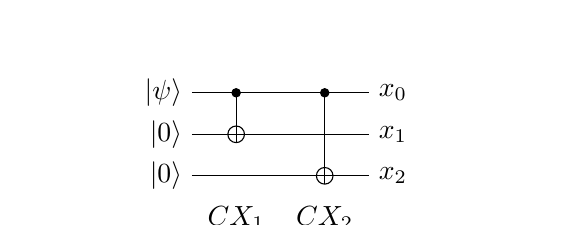
\begin{tikzpicture}[scale=1.000000,x=1pt,y=1pt]
\filldraw[color=white] (0.000000, -7.500000) rectangle (64.000000, 37.500000);
% Drawing wires
% Line 1: a1 W \ket{\psi} x_0
\draw[color=black] (0.000000,30.000000) -- (64.000000,30.000000);
\draw[color=black] (0.000000,30.000000) node[left] {$\ket{\psi}$};
% Line 2: a2 W \ket{0} x_1
\draw[color=black] (0.000000,15.000000) -- (64.000000,15.000000);
\draw[color=black] (0.000000,15.000000) node[left] {$\ket{0}$};
% Line 3: a3 W \ket{0} x_2
\draw[color=black] (0.000000,0.000000) -- (64.000000,0.000000);
\draw[color=black] (0.000000,0.000000) node[left] {$\ket{0}$};
% Done with wires; drawing gates
% Line 4: a1 +a2 width=20%% $CX_1$
\draw (16.000000, -7.500000) node[text width=144pt,below,text centered] {$CX_1$};
\draw (16.000000,30.000000) -- (16.000000,15.000000);
\filldraw (16.000000, 30.000000) circle(1.500000pt);
\begin{scope}
\draw[fill=white] (16.000000, 15.000000) circle(3.000000pt);
\clip (16.000000, 15.000000) circle(3.000000pt);
\draw (13.000000, 15.000000) -- (19.000000, 15.000000);
\draw (16.000000, 12.000000) -- (16.000000, 18.000000);
\end{scope}
% Line 5: a1 +a3 width=20%% $CS_2$
\draw (48.000000, -7.500000) node[text width=144pt,below,text centered] {$CX_2$};
\draw (48.000000,30.000000) -- (48.000000,0.000000);
\filldraw (48.000000, 30.000000) circle(1.500000pt);
\begin{scope}
\draw[fill=white] (48.000000, 0.000000) circle(3.000000pt);
\clip (48.000000, 0.000000) circle(3.000000pt);
\draw (45.000000, 0.000000) -- (51.000000, 0.000000);
\draw (48.000000, -3.000000) -- (48.000000, 3.000000);
\end{scope}
% Done with gates; drawing ending labels
\draw[color=black] (64.000000,30.000000) node[right] {$x_0$};
\draw[color=black] (64.000000,15.000000) node[right] {$x_1$};
\draw[color=black] (64.000000,0.000000) node[right] {$x_2$};
% Done with ending labels; drawing cut lines and comments
% Done with comments
\end{tikzpicture}
\end{center}
\Soln Let $\ket{\psi} = a\ket{0}+b\ket{1}$.  Our goal is to show that application of the diagrammed circuit maps $\ket{\psi}\ket{00} = a\ket{000}+b\ket{100}$ to $a\ket{000}+b\ket{111} = a\ket{0_L}+b\ket{1_L}$.  Note that $\ket{\psi}\ket{00} = \begin{bmatrix}a & 0 & 0 & 0 & b & 0 & 0 & 0\end{bmatrix}^T$, and $$CX_1 = \begin{bmatrix}1 & 0 & 0 & 0 & 0 & 0 & 0 & 0 \\ 0 & 1 & 0 & 0 & 0 & 0 & 0 & 0 \\ 0 & 0 & 1 & 0 & 0 & 0 & 0 & 0 \\ 0 & 0 & 0 & 1 & 0 & 0 & 0 & 0 \\ 0 & 0 & 0 & 0 & 0 & 0 & 1 & 0 \\ 0 & 0 & 0 & 0 & 0 & 0 & 0 & 1 \\ 0 & 0 & 0 & 0 & 1 & 0 & 0 & 0 \\ 0 & 0 & 0 & 0 & 0 & 1 & 0 & 0\end{bmatrix},\ 
CX_2 = \begin{bmatrix}1 & 0 & 0 & 0 & 0 & 0 & 0 & 0 \\ 0 & 1 & 0 & 0 & 0 & 0 & 0 & 0 \\ 0 & 0 & 1 & 0 & 0 & 0 & 0 & 0 \\ 0 & 0 & 0 & 1 & 0 & 0 & 0 & 0 \\ 0 & 0 & 0 & 0 & 0 & 1 & 0 & 0 \\ 0 & 0 & 0 & 0 & 1 & 0 & 0 & 0 \\ 0 & 0 & 0 & 0 & 0 & 0 & 0 & 1 \\ 0 & 0 & 0 & 0 & 0 & 0 & 1 & 0\end{bmatrix}.$$

So 
\begin{align*} CX_2CX_1\ket{\psi}\ket{00} &= \begin{bmatrix}1 & 0 & 0 & 0 & 0 & 0 & 0 & 0 \\ 0 & 1 & 0 & 0 & 0 & 0 & 0 & 0 \\ 0 & 0 & 1 & 0 & 0 & 0 & 0 & 0 \\ 0 & 0 & 0 & 1 & 0 & 0 & 0 & 0 \\ 0 & 0 & 0 & 0 & 0 & 1 & 0 & 0 \\ 0 & 0 & 0 & 0 & 1 & 0 & 0 & 0 \\ 0 & 0 & 0 & 0 & 0 & 0 & 0 & 1 \\ 0 & 0 & 0 & 0 & 0 & 0 & 1 & 0\end{bmatrix}\begin{bmatrix}1 & 0 & 0 & 0 & 0 & 0 & 0 & 0 \\ 0 & 1 & 0 & 0 & 0 & 0 & 0 & 0 \\ 0 & 0 & 1 & 0 & 0 & 0 & 0 & 0 \\ 0 & 0 & 0 & 1 & 0 & 0 & 0 & 0 \\ 0 & 0 & 0 & 0 & 0 & 0 & 1 & 0 \\ 0 & 0 & 0 & 0 & 0 & 0 & 0 & 1 \\ 0 & 0 & 0 & 0 & 1 & 0 & 0 & 0 \\ 0 & 0 & 0 & 0 & 0 & 1 & 0 & 0\end{bmatrix}\begin{bmatrix}a \\ 0 \\ 0 \\ 0 \\ b \\ 0 \\ 0 \\ 0\end{bmatrix} \\
&=\begin{bmatrix}a & 0 & 0 & 0 & 0 & 0 & 0 & b\end{bmatrix}^T \\ 
&= a\ket{000}+b\ket{111}
\end{align*}
as desired.
%!TeX root=../solnQCQI.tex

\chapter{Entropy and information}
\Textbf{11.1}
Fair coin:

\begin{align}
    H({1/2, 1/2}) = \left( - \frac{1}{2} \log \frac{1}{2} \right) \times 2 = 1
\end{align}


Fair die:
\begin{align}
    H(p) = \left( - \frac{1}{6} \log \frac{1}{6} \right) \times 6 = \log 6.
\end{align}


The entropy decreases if the coin or die is unfair.



\Textbf{11.2}

From assumption $I(pq) = I(p) + I(q)$.

\begin{align}
    \frac{\partial I(pq)}{\partial p} &= \frac{\partial I(p)}{\partial p} + 0 = \frac{\partial I(p)}{\partial p}\\
    \frac{\partial I(pq)}{\partial q} &= 0 + \frac{\partial I(q)}{\partial q} = \frac{\partial I(q)}{\partial q}
\end{align}


\begin{align}
    \frac{\partial I(pq)}{\partial p}
        &=  \frac{\partial I(pq)}{\partial (pq)} \frac{\partial (pq)}{\partial p}
        = q \frac{\partial I(pq)}{\partial(pq)}
    \Rightarrow \frac{\partial I(pq)}{\partial(pq)} = \frac{1}{q} \frac{\partial I(p)}{\partial p}\\
%
    \frac{\partial I(pq)}{\partial q}
        &=  \frac{\partial I(pq)}{\partial (pq)} \frac{\partial (pq)}{\partial q}
        = p \frac{\partial I(pq)}{\partial(pq)}
    \Rightarrow \frac{\partial I(pq)}{\partial(pq)} = \frac{1}{p} \frac{\partial I(q)}{\partial q}
\end{align}

Thus
\begin{align}
    \frac{1}{q} \frac{\partial I(p)}{\partial p} &= \frac{1}{p} \frac{\partial I(q)}{\partial q}\\
    \therefore~ p \frac{d I(p)}{d p} &= q \frac{d I(q)}{d q} ~~~\text{ for all } p,q \in [0,1].\\
\end{align}

Then $p (d I(p) / d p)$ is constant.

If $p (d I(p) / d p) = k$, $k \in \mathds{R}$.
Then $I(p) = k \ln p = k' \log p$ where $k' = k / \log e$.



\Textbf{11.3}
$H_{\text{bin}}(p) = - p\log p - (1-p) \log (1-p)$.

\begin{align}
    \frac{d H_{\text{bin}}(p)}{d p}
        &= \frac{1}{\ln 2} \left( - \log p - 1 + \log (1-p) + 1 \right)\\
        &= \frac{1}{\ln 2} \ln \frac{1-p}{p} = 0\\
    \Rightarrow \frac{1-p}{p} = 1\\
    \Rightarrow p = 1/2.
\end{align}


\Textbf{11.4}
\Textbf{11.5}

\begin{align}
    H\left( p(x,y) || p(x)p(y) \right)
        &= \sum_{x,y} p(x,y) \log \frac{p(x) p(y)}{p(x,y)}\\
        &= - H(p(x,y)) - \sum_{x,y} p(x,y) \log \left[ p(x)p(y) \right]\\
        &= - H(p(x,y)) - \sum_{x,y} p(x,y) \left[ \log p(x) + \log p(y) \right]\\
        &= - H(p(x,y)) - \sum_{x,y} p(x,y) \log p(x) - \sum_{x,y} p(x,y) \log p(y)\\
        &= - H(p(x,y)) - \sum_{x} p(x) \log p(x) - \sum_{y} p(y) \log p(y)\\
        &= - H(p(x,y)) + H(p(x)) + H(p(y))\\
        &= - H(X,Y) + H(X) + H(Y).
\end{align}

From the non-negativity of the relative entropy,
\begin{align}
    H(X) +  H(Y) - H(X,Y) \geq 0\\
    \therefore H(X) + H(Y) \geq H(X,Y).
\end{align}



\Textbf{11.6}
\begin{align}
    H(Y) + H (X, Y, Z) - H(X, Y) - H(Y, Z)  
        &= \sum_{x,y,z} p(x,y,z) \log \left( p(x,y)p(y,z)/p(y)p(x,y,z) \right) \\
        &\geq \frac{1}{\ln{2}} \sum_{x,y,z} p(x,y,z) \left[1-p(x,y)p(y,z)/p(y)p(x,y,z) \right] \\
        = \frac{1-1}{\ln{2}}
        = 0
\end{align}
The equality occurs if and only if $p(x,y)p(y,z)/p(y)p(x,y,z)=1$, which means a Markov chain condition of $Z \rightarrow Y \rightarrow X$; $p(x|y)=p(x|y,z)$ 
\Textbf{11.7}
\Textbf{11.8}
\Textbf{11.9}
\Textbf{11.10}
\Textbf{11.11}
\Textbf{11.12}
\Textbf{11.13}
\Textbf{11.14}
\Textbf{11.15}
\Textbf{11.16}
\Textbf{11.17}
\Textbf{11.18}
\Textbf{11.19}
\Textbf{11.20}
\Textbf{11.21}
\Textbf{11.22}
\Textbf{11.23}
\Textbf{11.24}
\Textbf{11.25}
\Textbf{11.26}

\Textbf{Problem 11.1}
\Textbf{Problem 11.2}
\Textbf{Problem 11.3}
\Textbf{Problem 11.4}
\Textbf{Problem 11.5}

%!TeX root=../solnQCQI.tex

\Textbf{12.31}
Eve makes her qubits entangled with $\ket{\beta_{00}}$, and gets $\rho^E$.
\begin{align}
\ket{ABE} = U\ket{\beta_{00}^{\otimes n}}\ket{0}_E\\
\rho^E = tr_{AB} (\ket{ABE} \bra{ABE})
\end{align}
Note that Eve's mutual information with Alice and Bob measurements does not depend on whether Eve measures $\rho^E$ before Alice and Bob's measurement or after.
So we can assume that Eve measures $\rho^E$ after Alice and Bob's measurement.
Alice and Bob measure their Bell state, getting binary string $\vec{k}$ as an outcome.
Let $\rho^E_k$ and $p_k$ are the corresponding Eve's states and probabilities.
Note,
\begin{align}
\rho_E = \sum_k p_k \rho^E_k.
\end{align}
Let $K$ is a variable of $\vec{k}$ and $e$ is an outcom of a measurement of $\rho^E$, and $E$ is its variable.  From Holevo bound, 
\begin{align}
H(K:E) \le S(\rho^E) - \sum_k p_k \rho^E_k \le S(\rho^E) = S(\rho).
\end{align}


\setcounter{chapter}{0}
%!TeX root=../solnQCQI.tex

\chapter{Fundamental Concepts}
\Textbf{1.1} Probabilistic Classical Deutsch-Jozsa Algorithm: Suppose that the problem is not to distinguish between the constant and balanced functions \textit{with certainty}, but rather, with some probability of error $\epsilon < 1/2$.  What is the performance of the best classical algorithm for this problem?
\Soln  To a mathematician, this problem is (\textit{slightly}) under-specified.  Missing is the probability that the function $f$ in question is balanced, vice constant.  We assume that both are \textbf{equally} likely, a priori.  The results when all balanced or constant functions are chosen from randomly are significantly different, and likely less interesting.
We describe \textit{an} algorithm and analyze the error rate, but make no effort to show that it is the \textit{best} algorithm, nor that this is the most effective analysis. Let $C$ be the event that $f$ is constant, and $B$ be the event that it is balanced.  By hypothesis $P(C)=P(B)=\frac12$, a  priori.  Evaluating $f$ provides information which can be used to update these prior probabilities.  Classically evaluating the function once, say at $x_0$, provides no useful information, since comparison of values is at the heart of this problem.  Evaluating $f$ twice, say at $x_0$ and $x_1$, can unambiguously determine if $f$ is balanced when their values disagree.  So, let's assume they agree.  We use Bayesian inference to iteratively update the probability that $f$ is constant, given $k$ successive measurements that agree.  In a convenient abuse of notation, let $P(E\ |\ k) = P\bigl(E\ |\ f(x_0) = \cdots = f(x_{k-1})\bigr)$, $P(k\ |\ E) = P\bigl(f(x_0) = \cdots = f(x_{k-1})\ |\ E\bigr)$, and $P(k) =  P\bigl(f(x_0) = \cdots = f(x_{k-1})\bigr)$, for $E=B,C$, and $k\in\mathbb{N}$.  We have $P(C\ |\ 0)=P(C\ |\ 1)=P(B\ |\ 0)=P(B\ |\ 1) = 1/2$.  Note also that $P(k\ |\ C) = 1$, since if $f$ is constant all evaluations (including the $k$ in question) will agree.
By Baye's theorem and the Law of Total Probability:
\begin{align*}
P(C\ |\  k)&=\ \ \ \ \ \ \ \ \ \ \ \ \ \ \ \ \ \ \frac{P(k\ |\  C)\cdot P(C\ |\ k-1)}{P(k)} \\
&=\frac{P(k\ |\ C)\cdot P(C\ |\ k-1)}{ P(C\ |\ k-1) \cdot P(k\ |\ C) +  P(B\ |\ k-1) \cdot P(k\ |\ B)}
\end{align*}

The formula above can be used to iteratively update $P(C,k)$, and hence $P(B,k)=1-P(C,k)$, but first we must discuss $P(k\ |\ B)$.  It is important to note that when this quantity is used to update $P(C\ |\ k)$, it is already known with certainty that $f(x_0) = \cdots = f(x_{k-2})$, \textit{i.e.} $P(k-1) = 1$.  $P(k\ |\ B)$ is the probability that, given this information, evaluating $f$ one more time, at $x_{k-1}$, yields another value in agreement with $f(x_0),\cdots,f(x_{k-2})$.   We evaluate this by separating the two possible outcomes of evaluation and counting the number of balanced functions satisfying the hypotheses that would produce them.   If $f(x_{k-1}) =  f(x_0)$, then $x_{k-1}$ is the $k$-th value on which $f$ agrees.  There are $\binom{n-k}{n/2-k}$ balanced functions which would produce this result, corresponding to the selections of $n/2-k$ more of the remaining $n-k$ values on which $f$ can agree.  If $f(x_{k-1})\neq f(x_0)$, then $f$ must still agree on $n/2-k+1$ of the remaining $n-k$ values.  There are $\binom{n-k}{n/2-k+1}$ balanced functions that would produce this result. So:
\begin{align*}
P(k,B)&=\frac{\binom{n-k}{n/2-k}}{\binom{n-k}{n/2-k}+\binom{n-k}{n/2-k+1}} = \frac{\binom{n-k}{n/2-k}}{\binom{n-k+1}{n/2-k+1}} =  \frac{n/2-k+1}{n-k+1} = \frac{n-2k+2}{2n-2k+2}
\end{align*}

We are finally in a position to calculate $P(C\ |\ k)$.  Unfortunately, for fixed $n$, the machinery above does not produce formulas of bounded complexity as $k$ grows.  Each formula will be a rational function with equal degree in numerator and denominator, but those degrees seem to be $\lfloor k/2\rfloor$.  The coefficients of the leading terms show some structure that can be used for asymptotic analysis, which we do below.  We illustrate the calculation of $P(C\ |\ 2)$, $P(C\ |\ 3)$, and $P(C\ |\ 4)$, and list formulas for $P(C\ |\ 5)$ through $P(C\ |\ 7)$ ,  then discuss the results and some experimental confirmation.

\begin{align*}
P(C\ |\  2)&=\frac{P(2\ |\ C)\cdot P(C\ |\ 1)}{ P(C\ |\ 1) \cdot P(2\ |\ C) +  P(B\ |\ 1) \cdot P(2\ |\ B)} \\
&=\frac{1\cdot\frac12}{\frac12\cdot1+\frac12\cdot\frac{n-2}{2n-2}} \\
&=\frac{1}{1+\frac{n-2}{2n-2}} \\
&=\frac{2n-2}{3n-4} \\
P(C\ |\ 3)&=\frac{P(3\ |\ C)\cdot P(C\ |\ 2)}{ P(C\ |\ 2) \cdot P(3\ |\ C) +  P(B\ |\ 2) \cdot P(3\ |\ B)} \\
&=\frac{1\cdot\frac{2n-2}{3n-4}}{\frac{2n-2}{3n-4}+\left(1-\frac{2n-2}{3n-4}\right)\cdot\frac{n-4}{2n-4}} \\
&=\frac{4n-4}{5n-8} \\
P(C\ |\ 4)&=\frac{P(4\ |\ C)\cdot P(C\ |\ 3)}{ P(C\ |\ 3) \cdot P(4\ |\ C) +  P(B\ |\ 3) \cdot P(4\ |\ B)} \\
&=\frac{1\cdot\frac{4n-4}{5n-8}}{\frac{4n-4}{5n-8}+\left(1-\frac{4n-4}{5n-8}\right)\cdot\frac{n-6}{2n-6}} \\
&=\frac{8n^2-32n+24}{9n^2-42n+48} \\
P(C\ |\ 5)&=\frac{16n^2-64n+48}{17n^2-78n+96} \\
P(C\ |\ 6)&=\frac{32n^3-288n^2+736n-480}{33n^3-312n^2+924n-960} \\
P(C\ |\ 7)&=\frac{64n^3-576n^2+1472n-960}{65n^3-606n^2+1768n-1920}
\end{align*}

There are clearly patterns, the most striking of which yields $P(C\ |\ k)\xrightarrow[n\shortrightarrow\infty]{}\frac{2^{k-1}}{2^{k-1}+1}$, that is, given $k\geq2$ evaluations in agreement, the probability that $f$ is constant is ${\sim}1-\frac{1}{2^{k-1}+1}$, at least for large $n$.  In the quantum context, where $n$ is likely to be exponential in the number of qubits, this asymptotic value would be approached rapidly.  To confirm this analysis, a python script is included in the repo which experimentally calculates empirical values of $P(C\ |\ k)$ for specified values of $n$ and $k$.  It also calculates the theoretical values, recursing over $k$, for comparison.  See \href{https://github.com/tlesaul2/SolutionQCQINielsenChuang/blob/master/Python/Problem1.1.py}{\texttt{<git repo>/Python/Problem1.1.py}}.

To answer the problem most directly, \textit{i.e.}, ``what is the performance of the best classical algorithm for this problem?'', let $n$ be fixed and $0<\epsilon<\frac{1}{2}$ be specified.  The ``performance'' of classically evaluating the function of $n$ inputs in order to declare it constant with error less than $\epsilon$  is equivalent to determining the number $k$ of evaluations in agreement after which the probability that $f$ is constant is greater than $1-\epsilon$.  Note that in no case is this number less than two.  The entries in the table below are such values, with rows indexed by $n$, and columns corresponding to exponentially decreasing values of $\epsilon$.  Specifically, column $i$ lists the values of $k$ corresponding to $\epsilon = 1/2^i$.  The maximum value of $k$  in each row is $n/2+1$, since this implies the function is constant.

% Note, the indexing in the \cline's is for the
\begin{adjustbox}{center}
\begin{tabular}{|c||c|c|c|c|c|c|c|c|c|c|c|c|c|c|c|c|c|c|c|c|}
\hline
$\epsilon=1/2^i; i=$ & 1 & 2 & 3 & 4 & 5 & 6 & 7 & 8 & 9 & 10 & 11 & 12 & 13 & 14 & 15 & 16 & 17 & 18 & 19 & 20  \\ \hline \hline
$n=6$ & 2 & 3 & 3 & 4 & $\shortrightarrow$ \\ \cline{1-8}
$n=8$ & 2 & 3 & 4 & 4 & 4 & 5 & $\shortrightarrow$ \\ \cline{1-9}
$n=10$ & 2 & 3 & 4 & 4 & 5 & 5 & 6 & $\shortrightarrow$ \\ \cline{1-11}
$n=12$ & 2 & 3 & 4 & 4 & 5 & 5 & 6 & 6 & 7 & $\shortrightarrow$\\ \cline{1-13}
$n=14$ & 2 & 3 & 4 & 5 & 5 & 6 & 6 & 7 & 7 & 7 & 8 & $\shortrightarrow$ \\ \cline{1-15}
$n=16$ & 2 & 3 & 4 & 5 & 5 & 6 & 6 & 7 & 7 & 8 & 8 & 8 & 9 & $\shortrightarrow$ \\ \cline{1-17}
$n=18$ & 2 & 3 & 4 & 5 & 5 & 6 & 7 & 7 & 8 & 8 & 8 & 9 & 9 & 9 & 10 & $\shortrightarrow$ \\ \cline{1-19}
$n=20$ & 2 & 3 & 4 & 5 & 6 & 6 & 7 & 7 & 8 & 8 & 9 & 9 & 9 & 10 & 10 & 10 & 11 & $\shortrightarrow$ \\ \hline
$n=22$ & 2 & 3 & 4 & 5 & 6 & 6 & 7 & 7 & 8 & 9 & 9 & 9 & 10 & 10 & 11 & 11 & 11 & 11 & 12 & $\shortrightarrow$ \\ \hline
$n=24$ & 2 & 3 & 4 & 5 & 6 & 6 & 7 & 8 & 8 & 9 & 9 & 10 & 10 & 11 & 11 & 11 & 12 & 12 & 12 & 12 \\ \hline
$n=26$ & 2 & 3 & 4 & 5 & 6 & 6 & 7 & 8 & 8 & 9 & 9 & 10 & 10 & 11 & 11 & 12 & 12 & 12 & 13 & 13 \\ \hline
$n=28$ & 2 & 3 & 4 & 5 & 6 & 7 & 7 & 8 & 8 & 9 & 10 & 10 & 11 & 11 & 12 & 12 & 12 & 13 & 13 & 13 \\ \hline
$n=30$ & 2 & 3 & 4 & 5 & 6 & 7 & 7 & 8 & 9 & 9 & 10 & 10 & 11 & 11 & 12 & 12 & 13 & 13 & 13 & 14 \\ \hline
$n=32$ & 2 & 3 & 4 & 5 & 6 & 7 & 7 & 8 & 9 & 9 & 10 & 11 & 11 & 12 & 12 & 13 & 13 & 13 & 14 & 14 \\ \hline
$n=34$ & 2 & 3 & 4 & 5 & 6 & 7 & 7 & 8 & 9 & 9 & 10 & 11 & 11 & 12 & 12 & 13 & 13 & 14 & 14  & 15 \\ \hline
$n=36$ & 2 & 3 & 4 & 5 & 6 & 7 & 7 & 8 & 9 & 10 & 10 & 11 & 11 & 12 & 12 & 13 & 13 & 14 & 14 & 15 \\ \hline
$n=38$ & 2 & 3 & 4 & 5 & 6 & 7 & 8 & 8 & 9 & 10 & 10 & 11 & 12 & 12 & 13 & 13 & 14 & 14 & 15 & 15 \\ \hline
$n=40$ & 2 & 3 & 4 & 5 & 6 & 7 & 8 & 8 & 9 & 10 & 10 & 11 & 12 & 12 & 13 & 13 & 14 & 14 & 15 & 15 \\ \hline
$n=42$ & 2 & 3 & 4 & 5 & 6 & 7 & 8 & 8 & 9 & 10 & 10 & 11 & 12 & 12 & 13 & 14 & 14 & 15 & 15 & 16 \\ \hline
$n=44$ & 2 & 3 & 4 & 5 & 6 & 7 & 8 & 8 & 9 & 10 & 11 & 11 & 12 & 13 & 13 & 14 & 14 & 15 & 15 & 16 \\ \hline
$n=46$ & 2 & 3 & 4 & 5 & 6 & 7 & 8 & 8 & 9 & 10 & 11 & 11 & 12 & 13 & 13 & 14 & 14 & 15 & 16 & 16 \\ \hline
$n=48$ & 2 & 3 & 4 & 5 & 6 & 7 & 8 & 8 & 9 & 10 & 11 & 11 & 12 & 13 & 13 & 14 & 15 & 15 & 16 & 16 \\ \hline
$n=50$ & 2 & 3 & 4 & 5 & 6 & 7 & 8 & 9 & 9 & 10 & 11 & 11 & 12 & 13 & 13 & 14 & 15 & 15 & 16 & 16 \\ \hline
$n=52$ & 2 & 3 & 4 & 5 & 6 & 7 & 8 & 9 & 9 & 10 & 11 & 12 & 12 & 13 & 14 & 14 & 15 & 15 & 16 & 17 \\ \hline
$n=54$ & 2 & 3 & 4 & 5 & 6 & 7 & 8 & 9 & 9 & 10 & 11 & 12 & 12 & 13 & 14 & 14 & 15 & 16 & 16 & 17 \\ \hline
$n=56$ & 2 & 3 & 4 & 5 & 6 & 7 & 8 & 9 & 9 & 10 & 11 & 12 & 12 & 13 & 14 & 14 & 15 & 16 & 16 & 17 \\ \hline
$n=58$ & 2 & 3 & 4 & 5 & 6 & 7 & 8 & 9 & 9 & 10 & 11 & 12 & 12 & 13 & 14 & 15 & 15 & 16 & 16 & 17 \\ \hline
$n=60$ & 2 & 3 & 4 & 5 & 6 & 7 & 8 & 9 & 9 & 10 & 11 & 12 & 13 & 13 & 14 & 15 & 15 & 16 & 17 & 17 \\ \hline
$n=62$ & 2 & 3 & 4 & 5 & 6 & 7 & 8 & 9 & 10 & 10 & 11 & 12 & 13 & 13 & 14 & 15 & 15 & 16 & 17 & 17 \\ \hline
$n=64$ & 2 & 3 & 4 & 5 & 6 & 7 & 8 & 9 & 10 & 10 & 11 & 12 & 13 & 13 & 14 & 15 & 15 & 16 & 17 & 17 \\ \hline
\end{tabular}
\end{adjustbox}
\\

Loosely, for small numbers of evaluations and large $n$, \textit{i.e} in the bottom left of the table, each exponential increase in the probability of being constant desired requires an additional evaluation.  Eventually, the combinatorial reduction in the number of remaining balanced functions allows additonal evaluations to reduce the error with which the function can be declared constant by several powers of 2, as often seen in the top right.  That is not to say that the probability is always reduced by at least a factor of 2.  In fact, note that $P(C\ |\ 1) = 1/2$, and $P(C\ |\ 2)\xrightarrow[n\shortrightarrow\infty]{}2/3$, so $\frac{1-P(C\ |\ 1)}{1-P(C\ |\ 2)}\xrightarrow[n\shortrightarrow\infty]{}3/2$. The second evaluation only reduces the probability that the function is balanced by a factor of ${\sim}1.5$ for large $n$.  Asymptotically, for $k\geq2$, note that $\frac{1-P(C\ |\ k+1)}{1-P(C\ |\ k)}\xrightarrow[n\shortrightarrow\infty]{}\frac{\frac{1}{2^k+1}}{\frac{1}{2^{k-1}+1}}=\frac{2^{k-1}+1}{2^k+1}<2$, so all $k$-th evaluations eventually reduce the probability of the function being balanced by less than a factor of $2$, for large enough $n$.  Theoretically, it is seemingly possible there's a case in which halving the probability of being balanced requires two additional evaluations.  That is, there could exist $n$ and an $\epsilon=\frac{1}{2^i}$ requiring $k$ measurements to declare the function constant with error less than $\epsilon$ and at least $k+2$ measurements to declare the function constant with error less than $\epsilon/2$.  However, attempts to search for such a pathological case have come up empty.  The asymptotic short-fallings are overcome by the combinatorial reduction fast enough, before a power of 1/2 straddles two values of $k$. It is likely that more careful analysis could refute the possibility rigorously.

We finish discussion of this problem with a (perhaps unnecessary) table of values of $P(C\ |\ k)$ for fixed $n$ and $k$ (programmatically constructed with the python script mentioned above, as was the previous table.)  Again, once $k=n/2+1$, the function must be constant, so all probabilities are 1.

\begin{landscape}
\begin{table}

\setlength\tabcolsep{2pt}
\renewcommand{\arraystretch}{1.125}
\begin{tabular}{|c||c|c|c|c|c|c|c|c|c|c}
\hline
$k$ & 2 & 3 & 4 & 5 & 6 & 7 & 8 & 9 & 10 \\ \hline \hline
$n=4$ & $\frac{3}{4}\simeq0.7500$ & $\frac{1}{1}\simeq1.0000$ & $\rightarrow$ \\ \cline{1-5}
$n=6$ & $\frac{5}{7}\simeq0.7143$ & $\frac{10}{11}\simeq0.9091$ & $\frac{1}{1}\simeq1.0000$ & $\rightarrow$ \\ \cline{1-6}
$n=8$ & $\frac{7}{10}\simeq0.7000$ & $\frac{7}{8}\simeq0.8750$ & $\frac{35}{36}\simeq0.9722$ & $\frac{1}{1}\simeq1.0000$ & $\rightarrow$ \\ \cline{1-7}
$n=10$ & $\frac{9}{13}\simeq0.6923$ & $\frac{6}{7}\simeq0.8571$ & $\frac{21}{22}\simeq0.9545$ & $\frac{126}{127}\simeq0.9921$ & $\frac{1}{1}\simeq1.0000$ & $\rightarrow$ \\ \cline{1-8}
$n=12$ & $\frac{11}{16}\simeq0.6875$ & $\frac{11}{13}\simeq0.8462$ & $\frac{33}{35}\simeq0.9429$ & $\frac{66}{67}\simeq0.9851$ & $\frac{462}{463}\simeq0.9978$ & $\frac{1}{1}\simeq1.0000$ & $\rightarrow$ \\ \cline{1-9}
$n=14$ & $\frac{13}{19}\simeq0.6842$ & $\frac{26}{31}\simeq0.8387$ & $\frac{143}{153}\simeq0.9346$ & $\frac{143}{146}\simeq0.9795$ & $\frac{429}{431}\simeq0.9954$ & $\frac{1716}{1717}\simeq0.9994$ & $\frac{1}{1}\simeq1.0000$ & $\rightarrow$ \\ \hline
$n=16$ & $\frac{15}{22}\simeq0.6818$ & $\frac{5}{6}\simeq0.8333$ & $\frac{13}{14}\simeq0.9286$ & $\frac{39}{40}\simeq0.9750$ & $\frac{143}{144}\simeq0.9931$ & $\frac{715}{716}\simeq0.9986$ & $\frac{6435}{6436}\simeq0.9998$ & $\frac{1}{1}\simeq1.0000$ & $\rightarrow$ \\ \hline
$n=18$ & $\frac{17}{25}\simeq0.6800$ & $\frac{34}{41}\simeq0.8293$ & $\frac{85}{92}\simeq0.9239$ & $\frac{34}{35}\simeq0.9714$ & $\frac{221}{223}\simeq0.9910$ & $\frac{442}{443}\simeq0.9977$ & $\frac{2431}{2432}\simeq0.9996$ & $\frac{24310}{24311}\simeq1.0000$ & $\frac{1}{1}\simeq1.0000$ \\ \hline
$n=20$ & $\frac{19}{28}\simeq0.6786$ & $\frac{19}{23}\simeq0.8261$ & $\frac{323}{351}\simeq0.9202$ & $\frac{646}{667}\simeq0.9685$ & $\frac{646}{653}\simeq0.9893$ & $\frac{323}{324}\simeq0.9969$ & $\frac{4199}{4202}\simeq0.9993$ & $\frac{8398}{8399}\simeq0.9999$ & $\frac{92378}{92379}\simeq1.0000$ \\ \hline
$n=22$ & $\frac{21}{31}\simeq0.6774$ & $\frac{14}{17}\simeq0.8235$ & $\frac{133}{145}\simeq0.9172$ & $\frac{57}{59}\simeq0.9661$ & $\frac{323}{327}\simeq0.9878$ & $\frac{1292}{1297}\simeq0.9961$ & $\frac{969}{970}\simeq0.9990$ & $\frac{4522}{4523}\simeq0.9998$ & $\frac{29393}{29394}\simeq1.0000$ \\ \hline
$n=24$ & $\frac{23}{34}\simeq0.6765$ & $\frac{23}{28}\simeq0.8214$ & $\frac{161}{176}\simeq0.9148$ & $\frac{161}{167}\simeq0.9641$ & $\frac{437}{443}\simeq0.9865$ & $\frac{437}{439}\simeq0.9954$ & $\frac{7429}{7439}\simeq0.9987$ & $\frac{14858}{14863}\simeq0.9997$ & $\frac{14858}{14859}\simeq0.9999$ \\ \hline
$n=26$ & $\frac{25}{37}\simeq0.6757$ & $\frac{50}{61}\simeq0.8197$ & $\frac{115}{126}\simeq0.9127$ & $\frac{230}{239}\simeq0.9623$ & $\frac{805}{817}\simeq0.9853$ & $\frac{575}{578}\simeq0.9948$ & $\frac{10925}{10943}\simeq0.9984$ & $\frac{2185}{2186}\simeq0.9995$ & $\frac{37145}{37149}\simeq0.9999$ \\ \hline
$n=28$ & $\frac{27}{40}\simeq0.6750$ & $\frac{9}{11}\simeq0.8182$ & $\frac{225}{247}\simeq0.9109$ & $\frac{270}{281}\simeq0.9609$ & $\frac{690}{701}\simeq0.9843$ & $\frac{345}{347}\simeq0.9942$ & $\frac{1035}{1037}\simeq0.9981$ & $\frac{1725}{1726}\simeq0.9994$ & $\frac{6555}{6556}\simeq0.9998$ \\ \hline
$n=30$ & $\frac{29}{43}\simeq0.6744$ & $\frac{58}{71}\simeq0.8169$ & $\frac{261}{287}\simeq0.9094$ & $\frac{261}{272}\simeq0.9596$ & $\frac{1305}{1327}\simeq0.9834$ & $\frac{1740}{1751}\simeq0.9937$ & $\frac{10005}{10027}\simeq0.9978$ & $\frac{10005}{10012}\simeq0.9993$ & $\frac{10005}{10007}\simeq0.9998$ \\ \hline
$n=32$ & $\frac{31}{46}\simeq0.6739$ & $\frac{31}{38}\simeq0.8158$ & $\frac{899}{990}\simeq0.9081$ & $\frac{899}{938}\simeq0.9584$ & $\frac{8091}{8234}\simeq0.9826$ & $\frac{8091}{8146}\simeq0.9932$ & $\frac{4495}{4506}\simeq0.9976$ & $\frac{13485}{13496}\simeq0.9992$ & $\frac{310155}{310232}\simeq0.9998$ \\ \hline
$n=34$ & $\frac{33}{49}\simeq0.6735$ & $\frac{22}{27}\simeq0.8148$ & $\frac{341}{376}\simeq0.9069$ & $\frac{2046}{2137}\simeq0.9574$ & $\frac{9889}{10071}\simeq0.9819$ & $\frac{1798}{1811}\simeq0.9928$ & $\frac{24273}{24338}\simeq0.9973$ & $\frac{5394}{5399}\simeq0.9991$ & $\frac{13485}{13489}\simeq0.9997$ \\ \hline
$n=36$ & $\frac{35}{52}\simeq0.6731$ & $\frac{35}{43}\simeq0.8140$ & $\frac{77}{85}\simeq0.9059$ & $\frac{22}{23}\simeq0.9565$ & $\frac{682}{695}\simeq0.9813$ & $\frac{1705}{1718}\simeq0.9924$ & $\frac{4495}{4508}\simeq0.9971$ & $\frac{12586}{12599}\simeq0.9990$ & $\frac{37758}{37771}\simeq0.9997$ \\ \hline
$n=38$ & $\frac{37}{55}\simeq0.6727$ & $\frac{74}{91}\simeq0.8132$ & $\frac{1295}{1431}\simeq0.9050$ & $\frac{259}{271}\simeq0.9557$ & $\frac{407}{415}\simeq0.9807$ & $\frac{1628}{1641}\simeq0.9921$ & $\frac{12617}{12656}\simeq0.9969$ & $\frac{11470}{11483}\simeq0.9989$ & $\frac{33263}{33276}\simeq0.9996$ \\ \hline
$n=40$ & $\frac{39}{58}\simeq0.6724$ & $\frac{13}{16}\simeq0.8125$ & $\frac{481}{532}\simeq0.9041$ & $\frac{1443}{1511}\simeq0.9550$ & $\frac{3367}{3435}\simeq0.9802$ & $\frac{481}{485}\simeq0.9918$ & $\frac{1221}{1225}\simeq0.9967$ & $\frac{814}{815}\simeq0.9988$ & $\frac{2294}{2295}\simeq0.9996$ \\ \hline
$n=42$ & $\frac{41}{61}\simeq0.6721$ & $\frac{82}{101}\simeq0.8119$ & $\frac{533}{590}\simeq0.9034$ & $\frac{1066}{1117}\simeq0.9543$ & $\frac{19721}{20129}\simeq0.9797$ & $\frac{19721}{19891}\simeq0.9915$ & $\frac{19721}{19789}\simeq0.9966$ & $\frac{1517}{1519}\simeq0.9987$ & $\frac{16687}{16695}\simeq0.9995$ \\ \hline
$n=44$ & $\frac{43}{64}\simeq0.6719$ & $\frac{43}{53}\simeq0.8113$ & $\frac{1763}{1953}\simeq0.9027$ & $\frac{3526}{3697}\simeq0.9537$ & $\frac{45838}{46807}\simeq0.9793$ & $\frac{22919}{23123}\simeq0.9912$ & $\frac{848003}{851063}\simeq0.9964$ & $\frac{848003}{849193}\simeq0.9986$ & $\frac{65231}{65265}\simeq0.9995$ \\ \hline
$n=46$ & $\frac{45}{67}\simeq0.6716$ & $\frac{30}{37}\simeq0.8108$ & $\frac{129}{143}\simeq0.9021$ & $\frac{387}{406}\simeq0.9532$ & $\frac{1763}{1801}\simeq0.9789$ & $\frac{35260}{35583}\simeq0.9909$ & $\frac{343785}{345077}\simeq0.9963$ & $\frac{22919}{22953}\simeq0.9985$ & $\frac{848003}{848479}\simeq0.9994$ \\ \hline
$n=48$ & $\frac{47}{70}\simeq0.6714$ & $\frac{47}{58}\simeq0.8103$ & $\frac{705}{782}\simeq0.9015$ & $\frac{141}{148}\simeq0.9527$ & $\frac{6063}{6196}\simeq0.9785$ & $\frac{2021}{2040}\simeq0.9907$ & $\frac{82861}{83184}\simeq0.9961$ & $\frac{414305}{414951}\simeq0.9984$ & $\frac{1077193}{1077839}\simeq0.9994$ \\ \hline
$n=50$ & $\frac{49}{73}\simeq0.6712$ & $\frac{98}{121}\simeq0.8099$ & $\frac{2303}{2556}\simeq0.9010$ & $\frac{658}{691}\simeq0.9522$ & $\frac{987}{1009}\simeq0.9782$ & $\frac{1974}{1993}\simeq0.9905$ & $\frac{14147}{14204}\simeq0.9960$ & $\frac{198058}{198381}\simeq0.9984$ & $\frac{4060189}{4062773}\simeq0.9994$ \\ \hline
$n=52$ & $\frac{51}{76}\simeq0.6711$ & $\frac{17}{21}\simeq0.8095$ & $\frac{833}{925}\simeq0.9005$ & $\frac{4998}{5251}\simeq0.9518$ & $\frac{11186}{11439}\simeq0.9779$ & $\frac{5593}{5648}\simeq0.9903$ & $\frac{50337}{50546}\simeq0.9959$ & $\frac{11186}{11205}\simeq0.9983$ & $\frac{28294}{28313}\simeq0.9993$ \\ \hline
$n=54$ & $\frac{53}{79}\simeq0.6709$ & $\frac{106}{131}\simeq0.8092$ & $\frac{901}{1001}\simeq0.9001$ & $\frac{901}{947}\simeq0.9514$ & $\frac{44149}{45161}\simeq0.9776$ & $\frac{25228}{25481}\simeq0.9901$ & $\frac{296429}{297694}\simeq0.9958$ & $\frac{592858}{593903}\simeq0.9982$ & $\frac{296429}{296638}\simeq0.9993$ \\ \hline
$n=56$ & $\frac{55}{82}\simeq0.6707$ & $\frac{55}{68}\simeq0.8088$ & $\frac{583}{648}\simeq0.8997$ & $\frac{583}{613}\simeq0.9511$ & $\frac{9911}{10141}\simeq0.9773$ & $\frac{4505}{4551}\simeq0.9899$ & $\frac{31535}{31673}\simeq0.9956$ & $\frac{12614}{12637}\simeq0.9982$ & $\frac{592858}{593295}\simeq0.9993$ \\ \hline
$n=58$ & $\frac{57}{85}\simeq0.6706$ & $\frac{38}{47}\simeq0.8085$ & $\frac{1045}{1162}\simeq0.8993$ & $\frac{1254}{1319}\simeq0.9507$ & $\frac{11077}{11337}\simeq0.9771$ & $\frac{11077}{11192}\simeq0.9897$ & $\frac{51357}{51587}\simeq0.9955$ & $\frac{85595}{85756}\simeq0.9981$ & $\frac{119833}{119925}\simeq0.9992$ \\ \hline
$n=60$ & $\frac{59}{88}\simeq0.6705$ & $\frac{59}{73}\simeq0.8082$ & $\frac{1121}{1247}\simeq0.8990$ & $\frac{2242}{2359}\simeq0.9504$ & $\frac{24662}{25247}\simeq0.9768$ & $\frac{12331}{12461}\simeq0.9896$ & $\frac{653543}{656533}\simeq0.9954$ & $\frac{59413}{59528}\simeq0.9981$ & $\frac{1010021}{1010826}\simeq0.9992$ \\ \hline
$n=62$ & $\frac{61}{91}\simeq0.6703$ & $\frac{122}{151}\simeq0.8079$ & $\frac{3599}{4005}\simeq0.8986$ & $\frac{3599}{3788}\simeq0.9501$ & $\frac{68381}{70019}\simeq0.9766$ & $\frac{273524}{276449}\simeq0.9894$ & $\frac{752191}{755701}\simeq0.9954$ & $\frac{752191}{753686}\simeq0.9980$ & $\frac{3624193}{3627183}\simeq0.9992$ \\ \hline
$n=64$ & $\frac{63}{94}\simeq0.6702$ & $\frac{21}{26}\simeq0.8077$ & $\frac{1281}{1426}\simeq0.8983$ & $\frac{549}{578}\simeq0.9498$ & $\frac{3599}{3686}\simeq0.9764$ & $\frac{3599}{3638}\simeq0.9893$ & $\frac{68381}{68706}\simeq0.9953$ & $\frac{478667}{479642}\simeq0.9980$ & $\frac{5265337}{5269822}\simeq0.9991$ \\ \hline

\end{tabular}
\end{table}
\end{landscape}






%%%%%%%%%%%%%%%%%%%%%%%%%%%%%%%%%%%%%%%%%%%%%%%%%%%%%%%%%%%%%%%%%%%%%%%%%%%%%

%参考文献
%\bibliographystyle{jplain}
%\bibliography{ref} % ref.bib を読み込み
\end{document}
